\documentclass[../../main.tex]{subfiles}
\begin{document}
\setcounter{footnote}{0} 

\newcommand{\ade}{\emph{autodE }}
\newcommand{\lmethod}{\emph{lmethod}}
\newcommand{\hmethod}{\emph{hmethod}}
\newcommand{\lmethodx}{\emph{lmethod }}
\newcommand{\hmethodx}{\emph{hmethod }}


\NewDocumentCommand{\code}{v}{%
	\texttt{\textcolor{black}{#1}}%
}

\section{Manuscript III}

\emph{autodE: Automated Calculation of Reaction Energy Profiles -- Application to Organic and Organometallic Reactions}


\subsection{Abstract}

Calculating reaction energy profiles to aid in mechanistic elucidation has long been the domain of the expert computational chemist. Here, we introduce \ade (\url{https://github.com/duartegroup/autodE}), an open-source Python package capable of locating transition states and minima and delivering a full reaction energy profile from 1D or 2D chemical representations. \ade is broadly applicable to study organic and organometallic reaction classes, including addition, substitution, elimination, migratory insertion, oxidative addition and reductive elimination; it accounts for conformational sampling of both minima and TSs, and is compatible with many electronic structure packages. The general applicability of \ade is demonstrated in complex multi-step reactions, including metal-catalysed cobalt- and rhodium-catalysed hydroformylation, and an Ireland-Claisen rearrangement.


\subsection{Introduction}


Automating the search for new chemical reactions is seen as one of the ‘grand challenges’ in computational chemistry.\cite{Grimme2018, Foscato2020} Discovering such thermodynamically and kinetically accessible reactions requires knowledge of the underlying potential energy surface (PES), which -- to a first approximation -- involves the characterization of reactants, products, intermediates, and transition states (TSs).\cite{Cheng2015, Sameera2012, Kozuch2011} While this has been routine for computational chemists for decades, locating TSs remains time consuming and a highly non-systematic endeavour.\cite{Simm2019} To this end, many automated TS-search algorithms have been developed which may be broadly classified into single and double-ended methods.\cite{Jensen2020, Dewyer2018} The former requires a single chemical structure from which TSs, intermediates, and products are located with no \emph{a priori} information. Representative examples include the ab initio nanoreactor (AINR),\cite{Wang2014} which employs high temperature and pressure molecular dynamics (MD) simulations to identify chemical transformations; the single-ended growing-string method (SE-GSM),\cite{Zimmerman2015} which iteratively generates structures along the PES and optimises them until a TS and minima at each side of the string are found; the artificial force induced reaction (AFIR) method,\cite{Maeda2016} which adds artificial external forces to the original PES of the target system, and the transition state search method which uses high-energy chemical dynamics simulations (CDS) and a geometry-based algorithm to identify reactive pathways.\cite{Martinez-Nunez2015} While they allow for free exploration of unknown pathways, these methods remain costly and limited to small systems ($\sim10$ reactant atoms) if left to explore all transformations.
\\\\
On the other hand, double-ended methods use knowledge of both reactants and products to generate TSs. Depending on the specific method either single or multiple steps can be studied. The latter includes reaction network enumeration algorithms, which allow for a systematic search of the reaction space, but hit an exponential wall of complexity if arbitrarily many intermediates are permitted.\cite{Kim2018, Habershon2016} Single-step methods, although seemingly limited in scope, remain a powerful and affordable approach to explore many chemical processes determined by elementary steps. This is the case, for example, when the goal is to elucidate the origin of regio- or enantioselectivity or compare different synthetically-plausible pathways for a given transformation. Several methods have been developed following this philosophy, from linear and quasi-synchronous transit\cite{Halgren1977, Peng1993} and related approaches\cite{Dewar1984, Elber1987} to more recent developments based on growing\cite{Dohm2020} and freezing string methods\cite{Suleimanov2015, Behn2011} (GSM/FSM, Figure \ref{fig::ade_1}). Finally, heuristic approaches guided by either graph-based chemical rules or electronic-structure theory have been employed to explore a wide range of chemical reactions; including the Reaction Mechanism Generator,\cite{Gao2016} which follows approaches pioneered by NetGen,\cite{Broadbelt1994} and other reaction network approaches.\cite{Rappoport2019, Bergeler2015}


\begin{figure}[h!]
	\vspace{0.4cm}
	\centering
	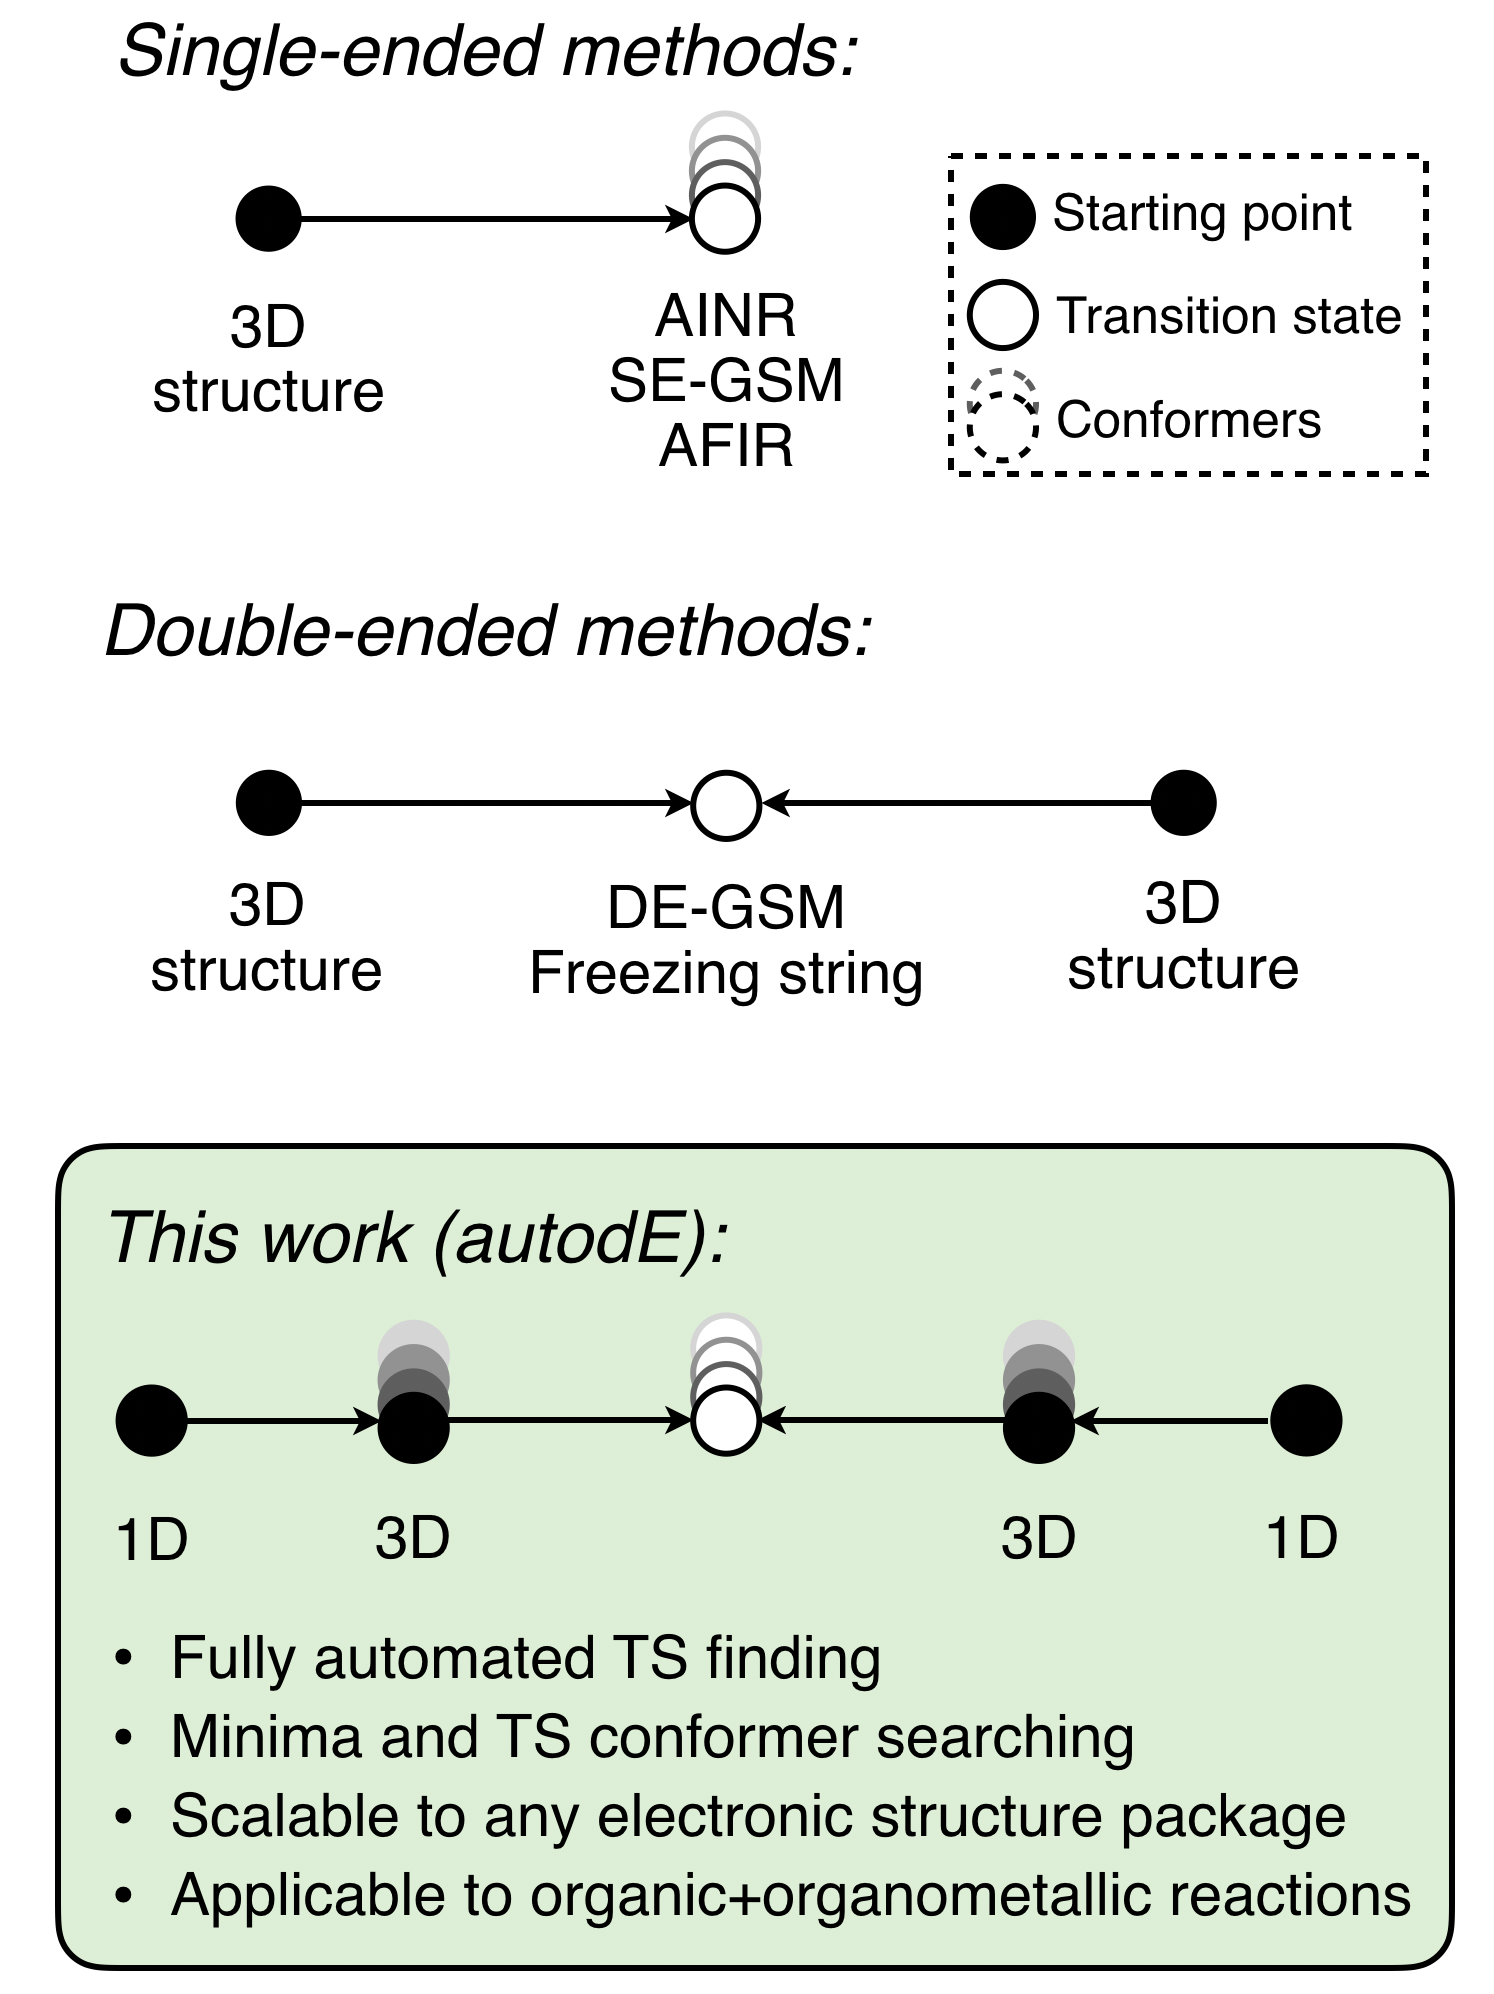
\includegraphics[width=7.5cm]{5/autode/figs/fig1}
	\vspace{0.4cm}
	\hrule
	\caption{Comparison of approaches to generate reaction profiles.}
	\label{fig::ade_1}
\end{figure}


Here, we introduce \emph{autodE}, which combines elements of previously reported double-ended methods with the development of a general, easy to use, and freely available package to automate the characterization of reaction pathways. The \ade algorithm takes inspiration from related methods, such as AutoTS\cite{Jacobson2017} developed by Schr\"{o}dinger\texttrademark $\,$ and the Reaction Mechanism Generator developed by Green et al.,\cite{Gao2016} and aims to overcome current limitations in applicability, conformational sampling and accessibility; specifically (1) it provides a broadly applicable framework to study organic and organometallic reaction classes; (2) it accounts for conformational sampling of both minima and transition states, which is essential particularly when exploring flexible systems; (3) it is freely available (open-source Python package distributed under an MIT license) and requires minimal user input and expertise. Moreover, it is compatible with several electronic structure theory packages and extensible to others. This work describes the algorithm and implementation of \ade and demonstrates its capabilities in a range of representative organic and organometallic reactions. We demonstrate that \ade is capable of locating the different TSs and minima along the PES and delivering a full reaction energy profile using only SMILES representations as inputs, available from most 2D chemical sketching software. To illustrate the functionality and general applicability of \emph{autodE}, we apply it to a range of reaction classes, including complex organic and metal-catalysed reactions.


\subsection{Methodology}

In general, human-guided characterization of TSs and reaction pathways requires: (1) locating reactants and products; (2) locating the TS, usually starting from a guess TS structure generated by chemical intuition; (3*) once reactants, TSs, and products have been characterized, perform a conformational search to identify the lowest energy conformer in each case; and (4*) performing single point energy evaluations to refine energies. While the starred steps are not always performed, they are usually necessary to achieve meaningful conclusion about the reactivity and selectivity of a given reaction step. Our method follows this workflow, which is described in detail in the following sections, along with representative examples (Figure \ref{fig::ade_2}).



\begin{sidewaysfigure}

	\vspace{0.2cm}
	\centering
	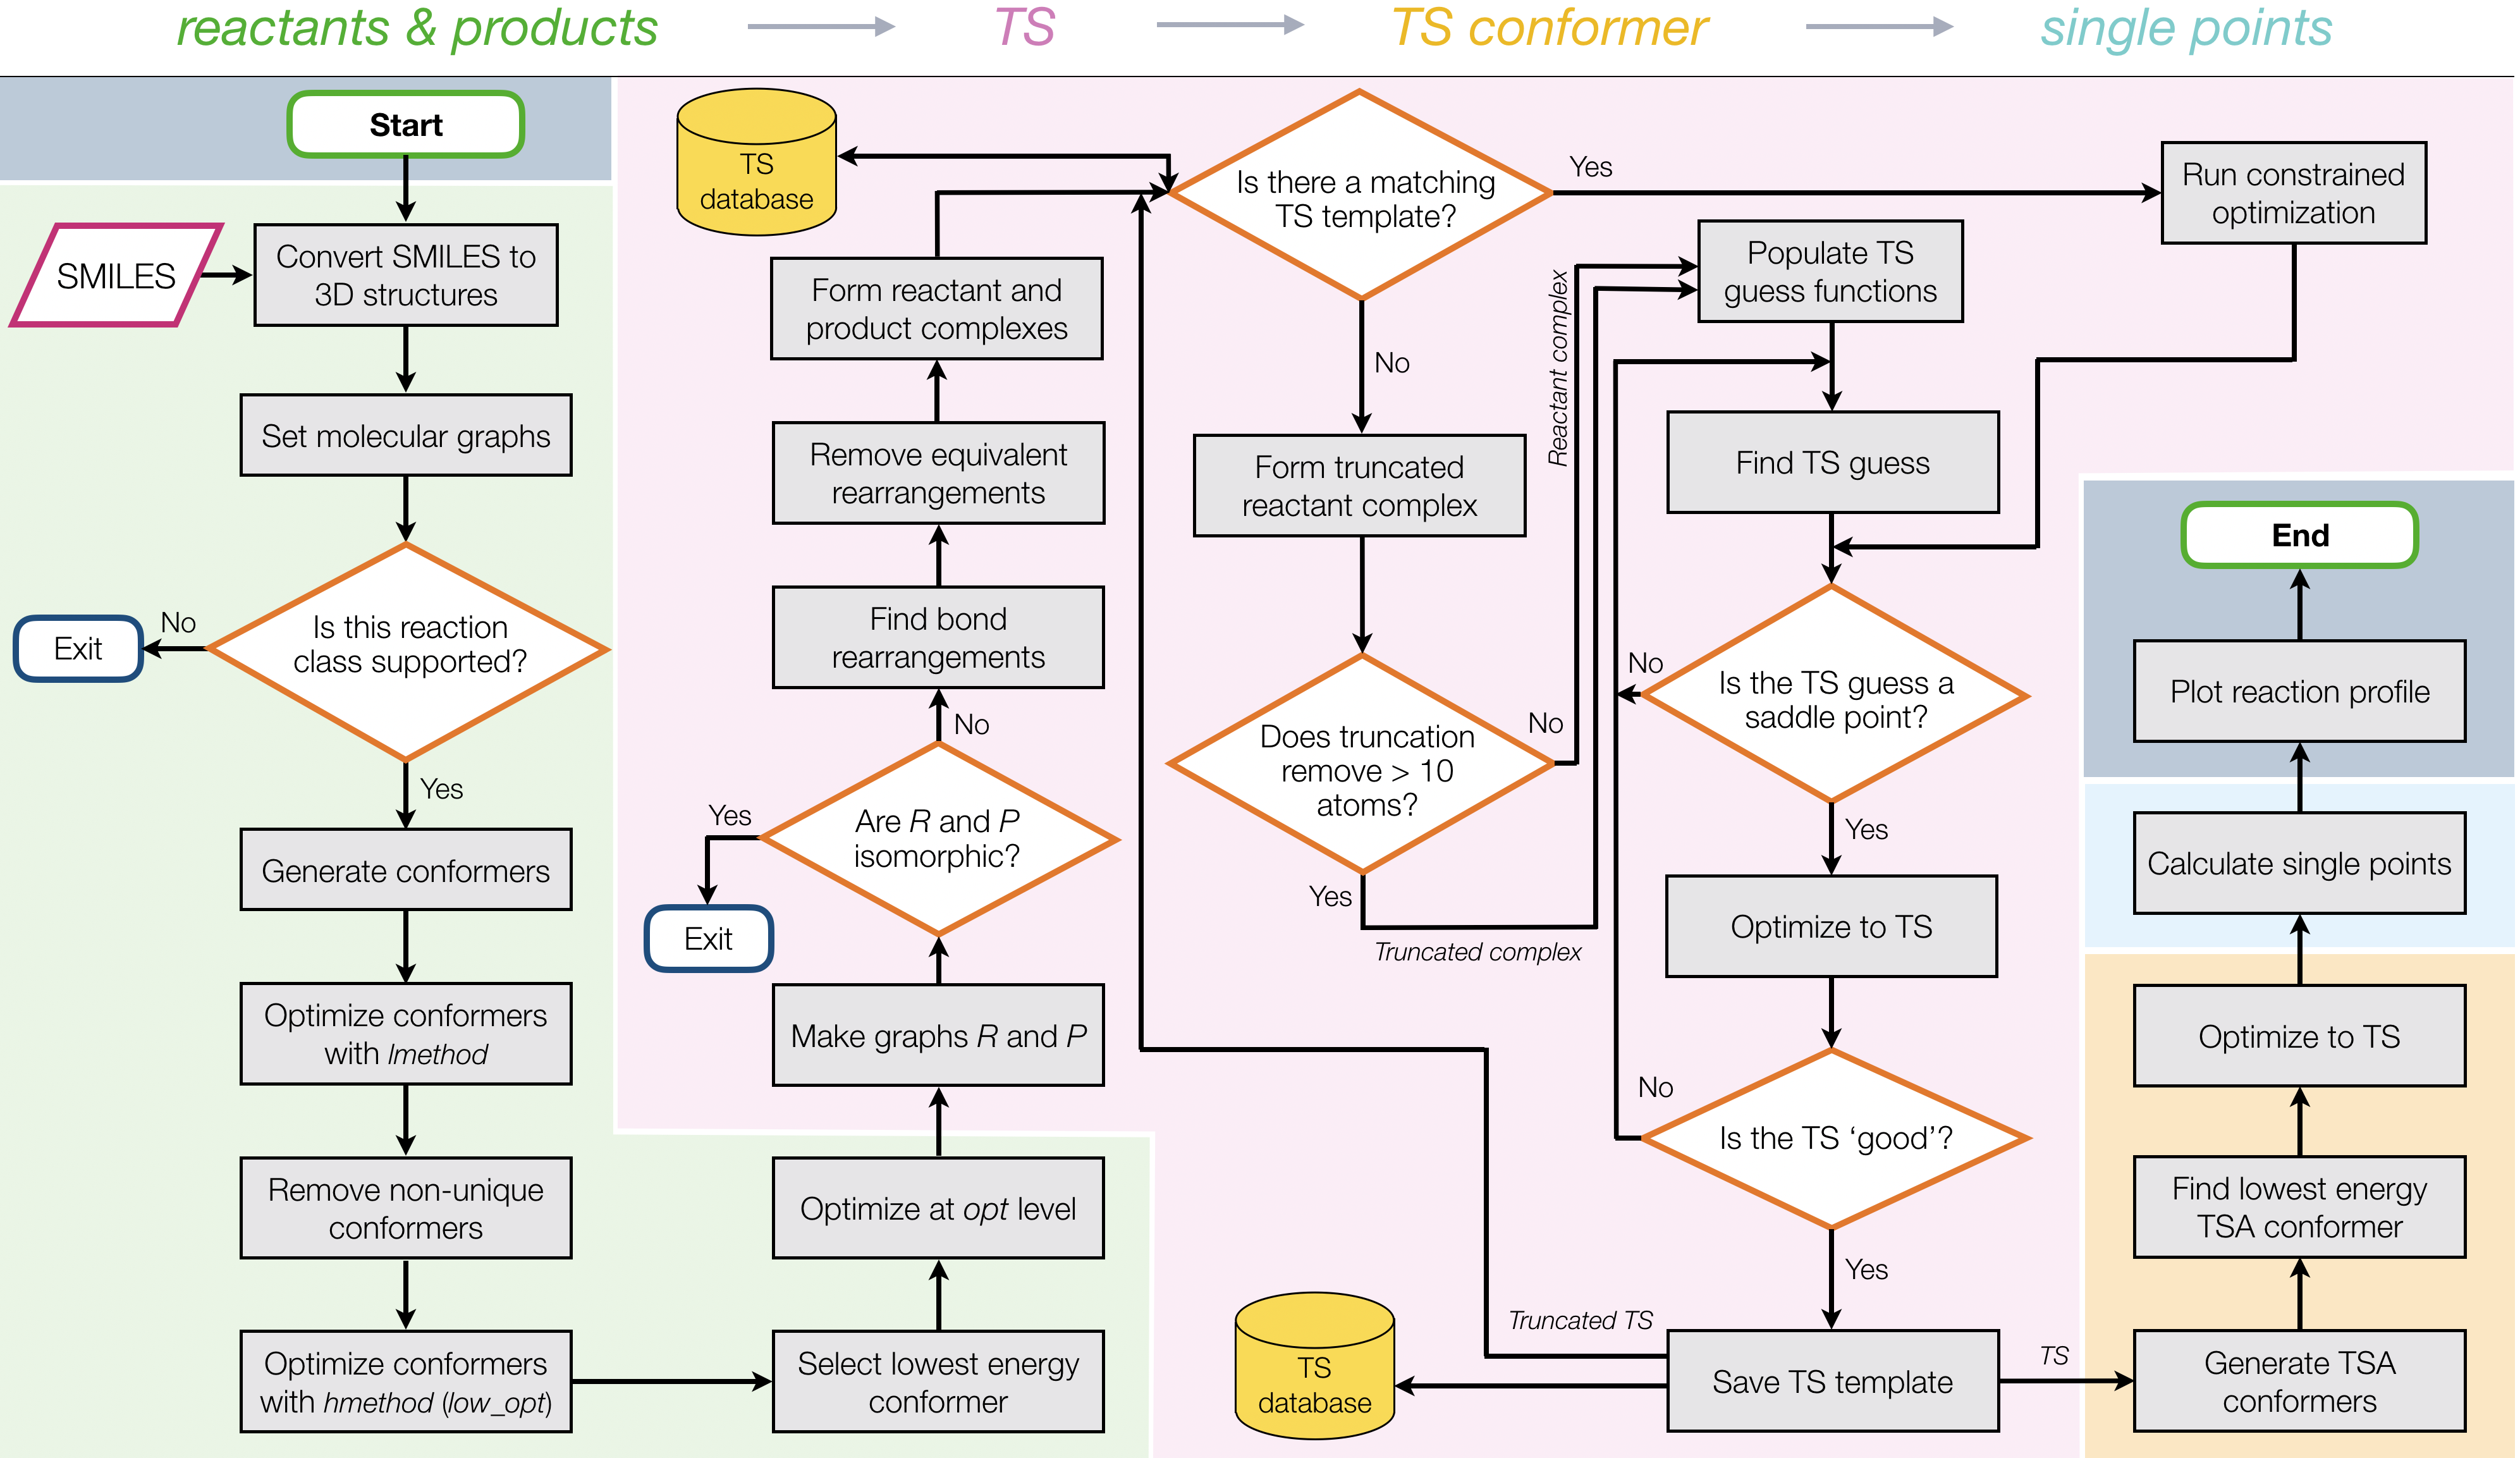
\includegraphics[width=\textwidth]{5/autode/figs/fig2}
	\vspace{0.2cm}
	\hrule
	\caption{Diagrammatic workflow used by \ade to generate a reaction profile from a set of reactant(s) and product(s) SMILES strings. TSA = transition state analogue, where active bonds are constrained at distances found at the TS found in previous the step.}
	\label{fig::ade_2}

\end{sidewaysfigure}

\newpage


With a view to generating reaction profiles efficiently using currently available quantum mechanics methods, our implementation makes use of two levels of theory: a lower-level (\lmethod) and higher-level method (\hmethod). Both methods have default settings (Table \ref{fig::ade_1}) selected based on their transferability, which can be modified by the user depending on the methods available in the respective software. For example, DFT methods can be used as \lmethodx for optimizations, and wavefunction (WF) methods for \hmethodx single point energy evaluations.



\begin{table}[h!]
	\def\arraystretch{2.0}
	\begin{tabularx}{\textwidth}{YYY}
		\hline
		Software Package &	Calculation	   & Default Method \\
		\hline
						& 	low\_opt &	PBE-D3BJ/def2-SVP
\\
		ORCA, Gaussian09, NWChem$^a$ & opt, optts, hess & 	PBE0-D3BJ/def2-SVP
 \\
						&sp	& PBE0-D3BJ/def2-TZVP
\\
		MOPAC&	low\_opt, opt, sp &	PM7
\\
		XTB		&low\_opt, opt, sp&	GFN2-XTB
\\
		
	\end{tabularx}
	\hrule
	\caption{Default methods used in \ade calculations. sp = single point energy, opt = optimization, low\_opt = low level optimization, optts = transition state optimization, hess = Hessian. \emph{a}. Uses D3 rather than D3BJ dispersion.}
	\label{table::ade_1}
\end{table}

\ade is readily extensible to many electronic structure theory codes and force fields in addition to those with currently implemented wrappers (Figure \ref{fig::ade_si_1a}). In the following paragraphs we describe the implementation and key features of \emph{autodE}. 

{\bfseries{Finding Lowest Energy Conformers for Reactant and Products}}. Locating the global minimum, or a structure close to it, on a PES is challenging but essential in estimating the feasibility of a reaction.\cite{Chan2019} To characterize the lowest energy conformer at a given level of theory requires transforming the 1D SMILES representation into a 3D geometry and searching the conformational space. Several open-source tools are available including RDKit\cite{Landrum2019} and CONFAB\cite{OBoyle2011} implemented in OpenBabel, but are generally limited to organic species. \ade uses the ETKDGv2\cite{Riniker2015} algorithm implemented in RDKit, which is known to perform well for organic species, along with its SMILES parser.\cite{Ebejer2012} To determine optimal parameters for the number of conformers generated and the root mean squared displacement (RMSD) threshold used to exclude identical conformers, a set of 20 amino acids were considered. Using CREST\cite{Pracht2020} as the benchmark method, the generation of 600 conformers and RMSD threshold = 0.1 \AA$;$ was sufficient to obtain reliable minima, rendering a conformer within 1 \kcalx of the most stable CREST conformer in 90\% of the cases (18/20, Figure \ref{fig::ade_si_2}). Therefore, this inexpensive conformer search was kept as the default for organic molecules and allows for \ade to remain method agnostic (i.e. \lmethod/\hmethodx can be chosen by the user). 

For metal complexes, where OpenBabel and RDKit fail to interpret the SMILES string and/or generate a sensible 3D geometry, we utilize our own (Open)SMILES parser and a simple repulsion+bonded (RB) forcefield (Eqn. \eqref{equation::ade_1}) by randomizing atoms then minimizing the function (Figure \ref{fig::ade_si_3}--\ref{fig::ade_si_5a}):
\begin{equation}
	U_\text{RB}(\boldsymbol{x}) = \sum_{ij}^\text{bonds} k_1 (r_{ij} - r_{ij}^\text{avg})^2 + \sum_{i > j} \frac{k_2}{r_{ij}^n}
	\label{equation::ade_1}
\end{equation}

For both organic molecules and metal complexes, the lowest energy conformer is found by optimizing each conformer at the \lmethodx and excluding non-unique structures based on an RMSD threshold (default 0.3 \AA), then an energy threshold (default 0.2 \kcal). The remaining structures are finally optimised at the desired low\_opt level with the \hmethod, and the lowest energy is kept (Figure \ref{fig::ade_si_6a}).  

{\bfseries{TS Location}}. Within \ade, each species has an associated molecular graph, in which the atoms correspond to vertices (V) and ‘bonds’ to edges (E). For a discussion of how bonds are defined, see the SI (Figure \ref{fig::ade_si_7}). From the set of reactant graphs $\{R_i\}$, the reactant graph ($R$) is formed as the graph union, and likewise with products $\{P_i\}$ to generate ($P$). This is represented in Figure \ref{fig::ade_3} for a Claisen rearrangement, where the graphs $R$ and $P$ are formed from a single reactant and product molecule. If $R$ and $P$ are isomorphic, as in an identity reaction, then the chemical transformation of interest is not obvious from the graph transformation and an exception is raised. Once this has been checked, to find an atom mapping (bijection) from $R$ to $P$, we generate a set of transformations of $R, \{R’\}$, obtained by adding and/or removing edges. This leads to a set of functions $\{g\}$ that represents all the possible bond rearrangements $[g: E(R) \rightarrow E(R’)]$.


The atom mapping(s) [$f: V(R’) \rightarrow V(P)$] are then found where $R’$ and $P$ are isomorphic using NetworkX.\cite{NetworkX} A brute force search for $\{g\}$, obtained by enumerating over all possible edge additions/deletions becomes intractable quickly, as the number of operations grows as $2^N$ for a system with $N$ atoms. However, chemical reactions usually involve a limited number of bonds that are formed and broken in a single elementary step, thereby substantially reducing the search space. We therefore limit the transformation to a maximum of four ‘active’ bonds where two edges are added and two removed, denoted (2, 2). For a graph $X$ with $b$ bonds ($b_X$ = $|E(X)|$) the principle of microscopic reversibility is used to switch reactants and products if $b_R < b_P$. 


\begin{figure}[h!]
	\vspace{0.4cm}
	\centering
	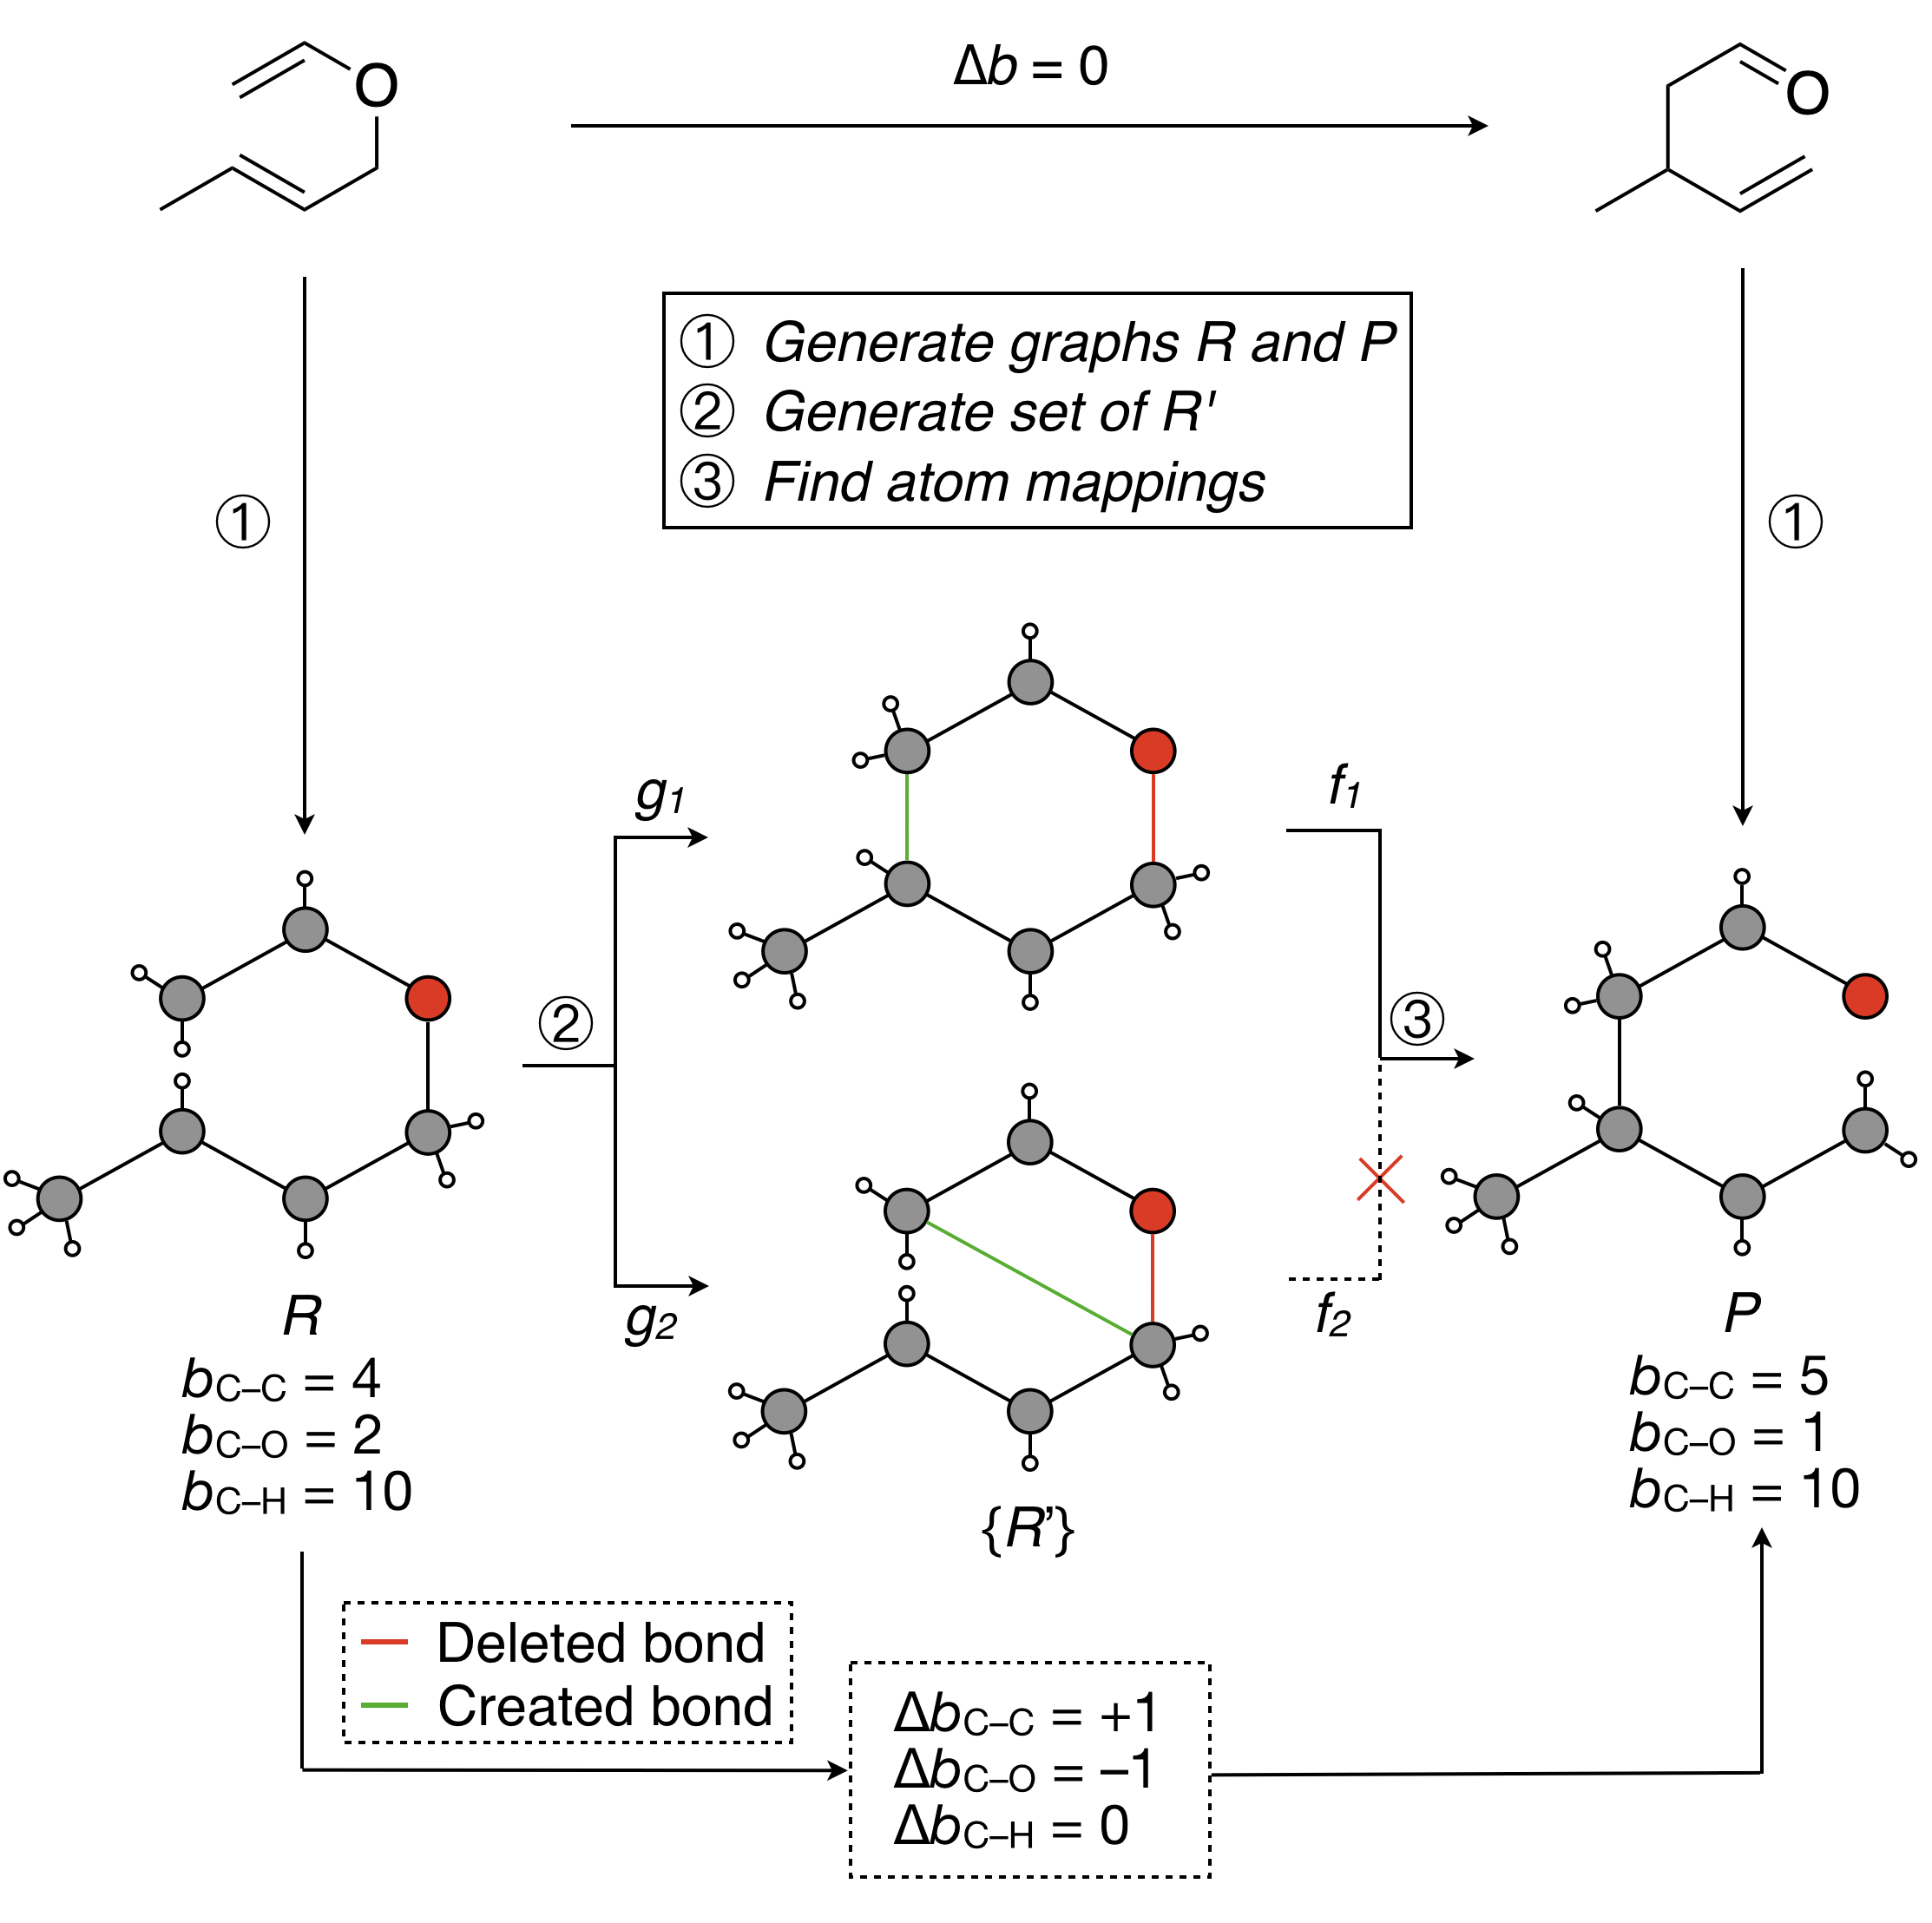
\includegraphics[width=11cm]{5/autode/figs/fig3}
	\vspace{0.4cm}
	\hrule
	\caption{Atom mappings between reactants and products for a Claisen rearrangement.}
	\label{fig::ade_3}
\end{figure}

\newpage
From these constraints, five scenarios exist: 

\begin{enumerate}[label=\Roman*.]
	\item (1, 1) – substitution reactions e.g., S${}_\text{N}$2.
	\item (2, 2) – substitution reactions e.g., epoxidation with peroxide.
	\item (0, 1) – dissociations e.g., E1 eliminations.
	\item (0, 2) – dissociations e.g., reverse of Diels-Alder cycloaddition.
	\item 	(1, 2) – eliminations e.g., E2 eliminations.
\end{enumerate}

Defining the change in the number of bonds as $\Delta b = b_R – b_P$ as in refs. \cite{Jacobson2017,Crabtree2009} only when $\Delta b = 0$ does the full set of deleting and adding two edges need to be enumerated. Further acceleration is achieved by calculating $\{\Delta b_k\}$ where $k$ is a bond type (e.g. C--C) and ensuring any atom ($a$) does not exceed a maximal valence (e.g., $d(a) \le 4$ for a carbon atom). For example, in a Claisen rearrangement $\Delta b_\text{C--C} = 1$ and $\Delta b_\text{C--O} = -1$ such that the enumeration over (1, 1) transformations is targeted to only C–C and C–O bonds (Figure \ref{fig::ade_3}). Once the set of valid $\{g\}$ is found, a TS is located for each of them (if it exists), and following conformational sampling, the lowest energy TS is taken for the calculation of a reaction profile. For the Claisen reaction shown in Figure \ref{fig::ade_3}, only one bond rearrangement is obtained while for the all-carbon analogue (O $\rightarrow$ CH$_2$) two rearrangements are found ($g = \{g_1, g_2\}$). While reasonably exhaustive, we are yet to find a reaction where the process of generating/checking $R’$ and $P$ isomorphisms and finding the mapping is comparable or more demanding than a DFT calculation.

To generate a saddle point, while ensuring compatibility with multiple electronic structure codes, we favour finding a TS guess by performing a set of constrained geometry optimizations along a linear path between reactants and products. In general, \ade attempts 1D constrained searches over forming/breaking bonds except when $\Delta b$ = 2 (e.g., Diels-Alder). If this procedure fails and the number of active bonds is more than one, a 2D PES exploration is performed by constrained optimizations and fitting a polynomial up to order 3.\cite{SciPy} From a 2D PES, the lowest energy saddle point is found by locating where the first derivative vanishes, and then using Dijkstra's algorithm\cite{Dijkstra1959} implemented in NetworkX.\cite{NetworkX} A constrained optimization at the saddle point is then performed to generate the TS guess. Once the TS guess is obtained, it is optimised with the TS optimisers implemented in the electronic structure theory package selected by the user. ‘Goodness’ of the TS is defined by a significant imaginary mode ($|\nu_\text{imag}| > 45$ cm$^{-1}$) and a significant contribution from the active bonds, or forward/backward displacement along the mode affording graphs isomorphic to reactants/products (quick reaction coordinate calculation,\cite{Goodman2003} see description of \code{true_ts()} function in §\ref{section::ade_si_algorithm} for further details). In cases where the reactant or product(s) are not isomorphic to $R$ or $P$ (e.g. barrierless proton transfers), rigid-body conformers of the reactant- and product- complex are generated (see SI §\ref{section::ade_si_nci_complexes}) and isomorphisms checked for the forwards/backwards displaced structures to all optimised conformers. We envisage the implementation of nudged elastic band (NEB) approaches to accelerate the computationally intensive 2D PES scans using an initial a linear path from the reactant(complex) by making/breaking bonds to drive towards a product state.


{\textbf{Truncation}}. Performing tens of constrained optimizations along one or two coordinates in a large system is currently computationally demanding. To accelerate the generation of a TS guess in such systems, the system is truncated. Our implementation truncates over C--X bonds where the carbon atom is fully saturated and is at least two bonds away from the active atoms, and the truncated group is replaced by a hydrogen atom (Figure \ref{fig::ade_si_8}). The TS is then located using this truncated complex and saved in the template library from which the full non-truncated TS may be found using the templating method described below. For truncation to be utilised it must remove $>10$ atoms. 


{\textbf{Finding Lowest Energy TS Conformers}}. TS conformers are located in a similar manner to the protocol described for metal complexes in §\ref{section::ade_si_metal_complex_confs} ($n$=8 in Eqn. \eqref{equation::ade_1} and randomization using a displacement vector of $~ 3$ \AA). However, here the ‘active’ bonds are constrained at distances found at the TS using a harmonic potential with a force constant $k_1’ = 10k_1$ (Eqn. \eqref{equation::ade_2}).
\begin{equation}
	U_\text{RB'}(\boldsymbol{x}) = \sum_{ij \in \text{bonds}} k_1 (r_{ij} - r_{ij}^\text{avg})^2 + \sum_{ij \in \text{const.}} k_1' (r_{ij} - r_{ij}^\text{avg})^2 + \sum_{i > j} \frac{k_2}{r_{ij}^8}
	\label{equation::ade_2}
\end{equation}

An identical method is then used to find the lowest energy transition state analogue (TSA) -- as a model for the TS -- by performing optimizations with the active bonds constrained to their length in the TS. From the TSA a TS is found by rerunning the transition state optimization and checking that it is both a ‘good’ TS and is lower in energy than the previously found TS.


{\bfseries{Transition State Templates}}. To accelerate the location of TSs, if available, a template is employed to generate a TS guess structure. Templates are saved into a local library following the successful location of a TS and contain a graph, solvent, charge and multiplicity. For a template to be used, the reactant (complex) must have the same charge, multiplicity, and solvent parameters as the one used to obtain the template. In addition, the active bonds must match (same number and atoms) along with their nearest neighbours, based on their connectivity and atom type. If a matching template is found in the library, then a TS guess is generated by constrained optimization, where the active bonds are fixed at values found in the saved TS, from which TS optimization is performed. For example, a TS found for EtCl + F$^{-}$ $\rightarrow$ EtF + Cl$^{-}$ enables a $10\times$ faster characterization of the TS for the propyl analogue. 


{\bfseries{Reactive Reactant Complexes}}. For bimolecular reactions (substitution and elimination, not addition as $b_P > b_R$) an initial association complex on the PES must be found that favours a linear arrangement of the nucleophile and the leaving group, while also reducing the required number of optimizations. For this reason, the energy function $U_\text{RR}$ (Eqn. \eqref{equation::ade_3}) is minimized with respect to rigid-body rotation and translation of one reactive component with empirical parameters $c_1 = c_2 = c_3 = 1, c_4 = 10$ and $c_5 = 2.5 (1.5)$ for charged (uncharged) complexes. 
\begin{equation}
	U_\text{RR}(\boldsymbol{x}_i) = \sum_\text{\{ac\}} c_1 (r_\text{ac} - c_5 r_\text{ac}^\text{avg})^2 + \sum_\text{\{acx\}} c_2 (1 - \cos\theta) + \sum_\text{\{acx\}} c_3 (1 - \cos\phi) + \sum_\text{\{ij\}} \frac{c_4}{r_\text{ij}^4}
	\label{equation::ade_3}
\end{equation}


\begin{figure}[h!]
	\vspace{0.4cm}
	\centering
	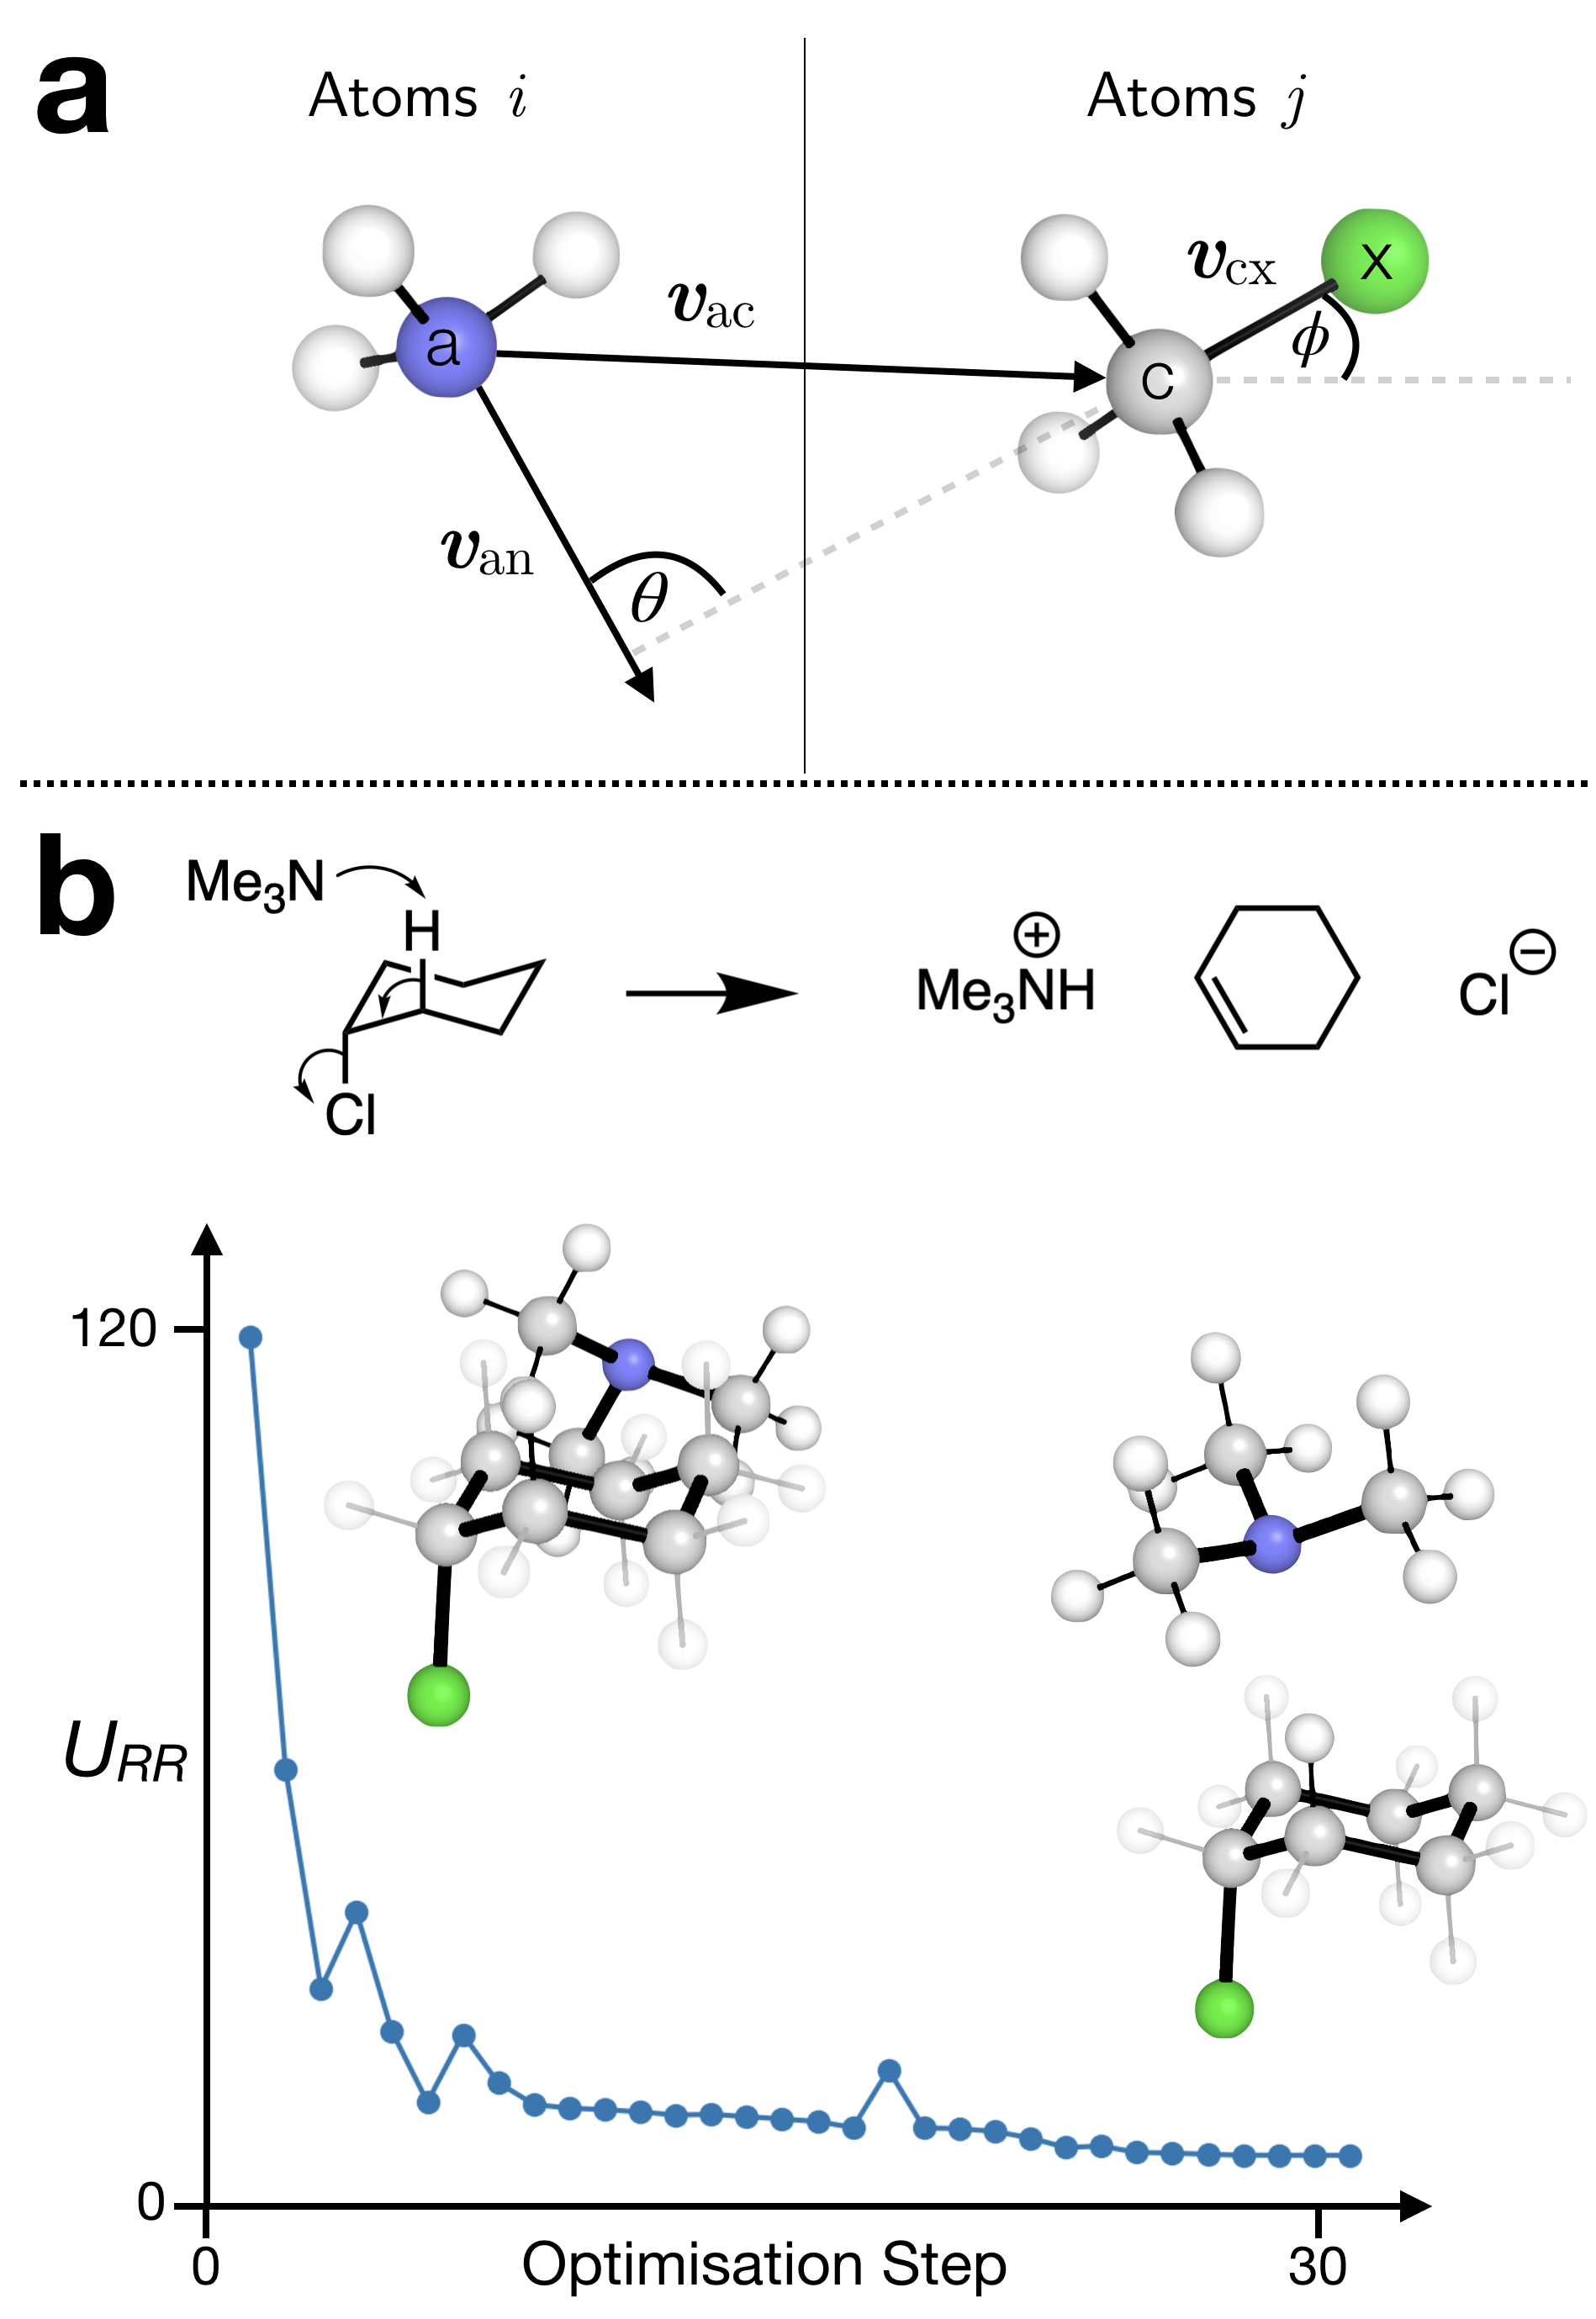
\includegraphics[width=8cm]{5/autode/figs/fig4}
	\vspace{0.3cm}
	\hrule
	\caption{(a) Illustration of the geometric parameters used in Eqn. \eqref{equation::ade_2} the S$_\text{N}$2 reaction NH$_3$ + CH$_3$Cl as an example: van is the average of vectors $\{\boldsymbol{v}_{am}\}$ where m is a nearest neighbour to a. (b) Minimization of $U_\text{RR}$  for an E2 reaction.}
	\label{fig::ade_4}
\end{figure}

This energy function has been designed to maximize the collinearity of vectors $\boldsymbol{v}_{an}$, $\boldsymbol{v}_{ac}$ and $\boldsymbol{v}_{cx}$ while maintaining both a low steric repulsion and distance ($r_{ac} = |\boldsymbol{v}_{ac}|$) close to that desired (Figure \ref{fig::ade_4}). This choice is guided by chemical intuition, and there are rare cases where this is not adhered to (e.g., front-side S$_\text{N}$2,\cite{Hamlin2018} which is found upon TS conformer searching). For example, adequate initial geometries are obtained for S${}_\text{N}2$ substitution, E2 elimination and S$_\text{N}$Ar reactions (Figure \ref{fig::ade_4}, \ref{fig::ade_si_9}). Note that there may be several minima on this surface; thus, multiple initial random rotations and translations ($\sim 10$) are performed to have a better chance of locating the global minimum while remaining computationally inexpensive (execution time $\sim$ seconds). Non-reactive association complex conformers are also available from optimization of random molecular orientations (SI §\ref{section::ade_si_nci_complexes}).


\subsection{Results and Discussion}

To demonstrate the applicability of \ade in multiple reaction classes, we explored some textbook organic reactions (e.g., S$_\text{N}$2, E2, etc.) alongside industrially relevant organic and metal-catalysed reactions involving more than 50 atoms. By way of example, we demonstrate that \ade is broadly applicable, efficient in exploring conformational space, and straightforward to use.

Even with a small amount of programming experience, using \ade is as simple as declaring reactants and products involved in the reaction from their respective SMILES strings, then calling a method. An input for calculating an S${}_\text{N}2$ reaction profile immersed in an implicit aqueous environment is shown in Figure 5. Here, by calling the method  \\
\code{calculate_reaction_profile} with complexes turned on, the association complexes are also calculated along the energy profile. Alternatively, one can decide only to obtain the TS, with the function  \code{locate_transition_state}.

Without specifying which electronic structure codes to use, \ade employs the first available \hmethodx and \lmethod, (sequentially ORCA, Gaussian09, NWChem and XTB, MOPAC respectively), with the default DFT methodologies listed in Table \ref{table::ade_1}. Using this setup, the reaction energy profile shown in Figure \ref{fig::ade_5} is obtained in about 30 minutes. While it would be ideal to obtain reaction free energies, the cost and limitations associated with the calculation of entropy and thermal contributions using currently available models (ideal gas) mean that the addition of such corrections should be considered with care. For this reason, potential energies are set as the default in \ade, but free energies are available with the \code{free_energy=True} flag. Further algorithmic details are outlined in the SI (§\ref{section::ade_si_algorithm}).


\begin{figure}[h!]
	\vspace{0.4cm}
	\centering
	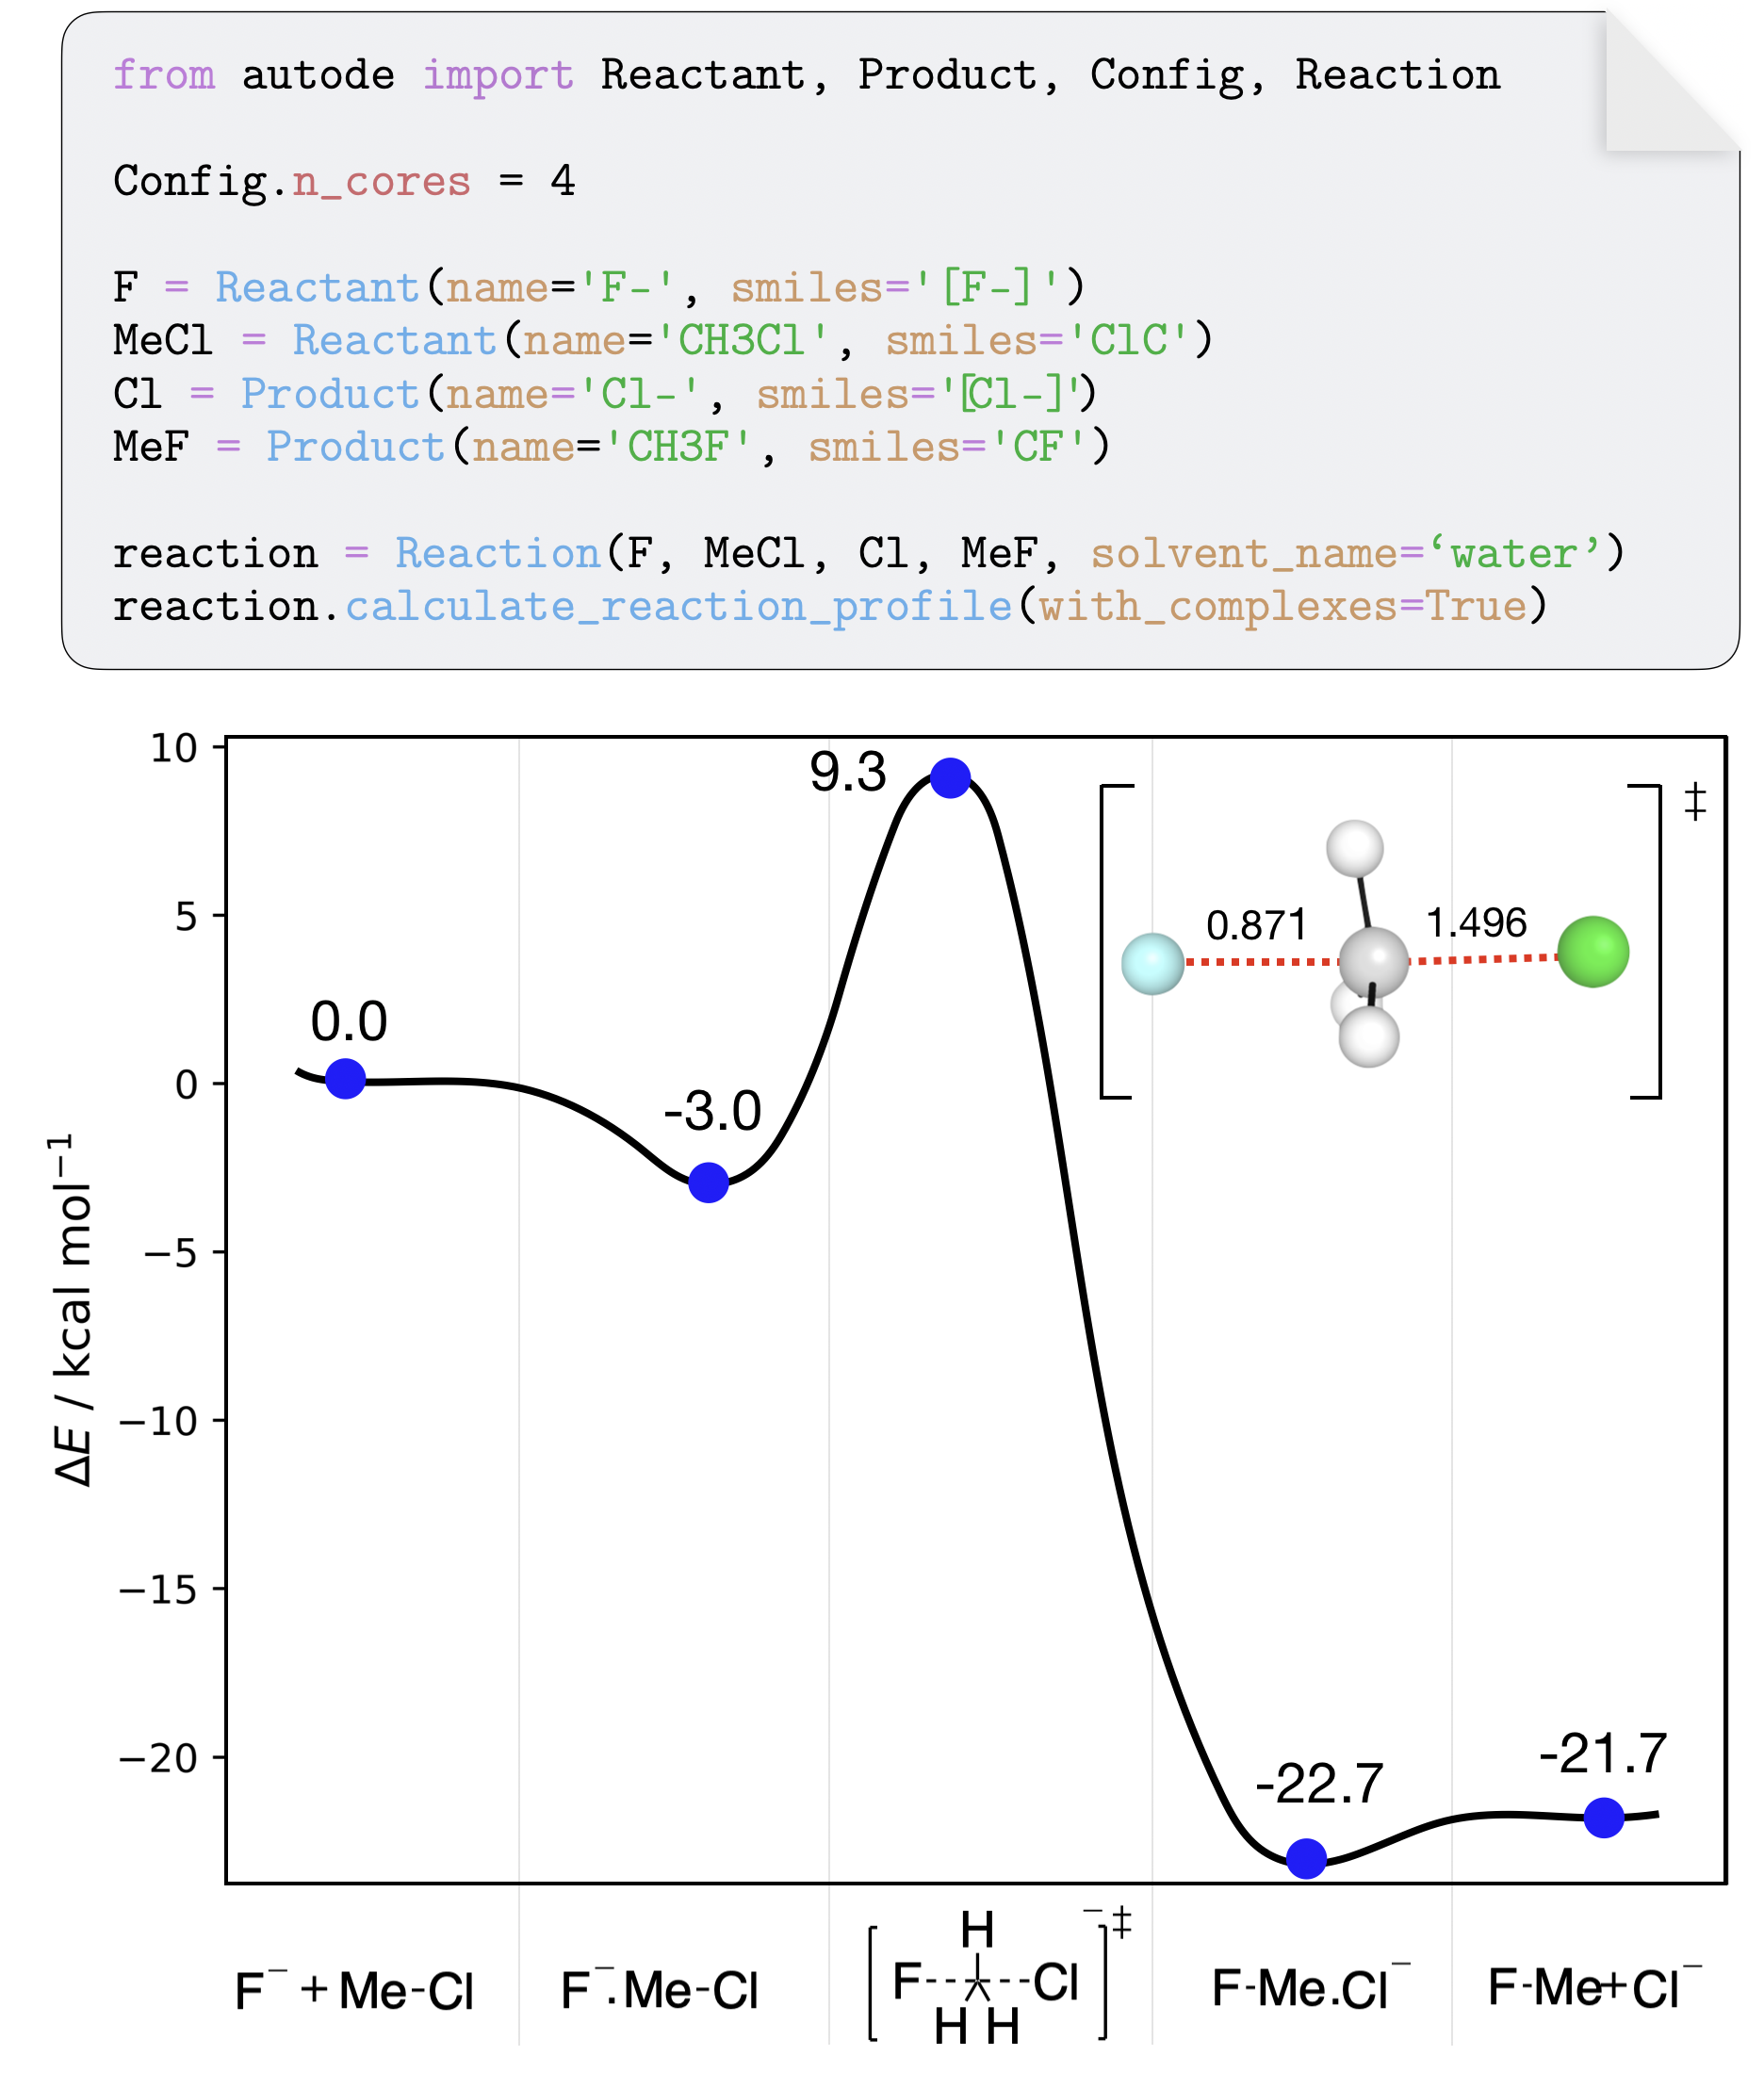
\includegraphics[width=10cm]{5/autode/figs/fig5}
	\vspace{0.4cm}
	\hrule
	\caption{Reaction energy profile for an S$_\text{N}$2 reaction calculated using \ade with GFN2-XTB and DFT level \lmethod/\hmethod in XTB/ORCA. Final energies quoted at the CPCM(H$_2$O)-PBE0-D3BJ/def2-TZVP//CPCM(H2O)-PBE0-D3BJ/def2-SVP level of theory and distances quoted in \AA.}
	\label{fig::ade_5}
\end{figure}

{\bfseries{TS Conformers}}. A thorough exploration of the conformational space in order to find the lowest energy conformer for reactants and TSs is essential in characterising the kinetic and thermodynamic parameters of a reaction. \ade provides two routes to locating TS conformers. The first uses reactant/product complex conformers, from which different TSs may be traversed, and the second locates TS conformers directly. If using templates, both approaches are efficient, generally requiring only one constrained optimisation and one TS optimisation per conformer once a TS has been found. Direct TS conformer searching is, however, faster as only the TSAs are optimised and the lowest energy found whereas full enumeration from reactant/product complexes can require rescanning over the PES.


For example, for an E2 elimination reaction, the initial search may locate a transition state in which the deprotonation occurs with the proton and the leaving group in a \emph{syn} conformation, rather than the favoured \emph{anti} conformer. The latter TS is automatically found in \ade by randomizing and minimizing Eqn. \eqref{equation::ade_2} (Figure \ref{fig::ade_6}a). Similarly, the \ade algorithm correctly locates the lowest energy H-migration TS for the radical decomposition of 1-propanol, with an RMSD $< 0.1$ \AA$\;$compared to the human-generated TS from ref. \cite{Ferro-Costas2018} (Figure \ref{fig::ade_si_13}). The importance of this unbiased TS conformer generation is highlighted in the Michael addition of nitromethyl acetate and methyl vinyl ketone, where several rotatable bonds exist (Figure \ref{fig::ade_6}b). For this reaction, an exhaustive search from product conformers generated 21 TS conformers, which upon optimization, led to a range in activation energies of more than 5 \kcalx and reaction energies that differ by up to 17 \kcal. The weak correlation between $\Delta E^\ddagger$ and $\Delta E_r$ from the global reactant conformer to each TS-product conformer pair highlights the importance of a systematic conformer search at both minima and transition states.


\begin{figure}[h!]
	\vspace{0.4cm}
	\centering
	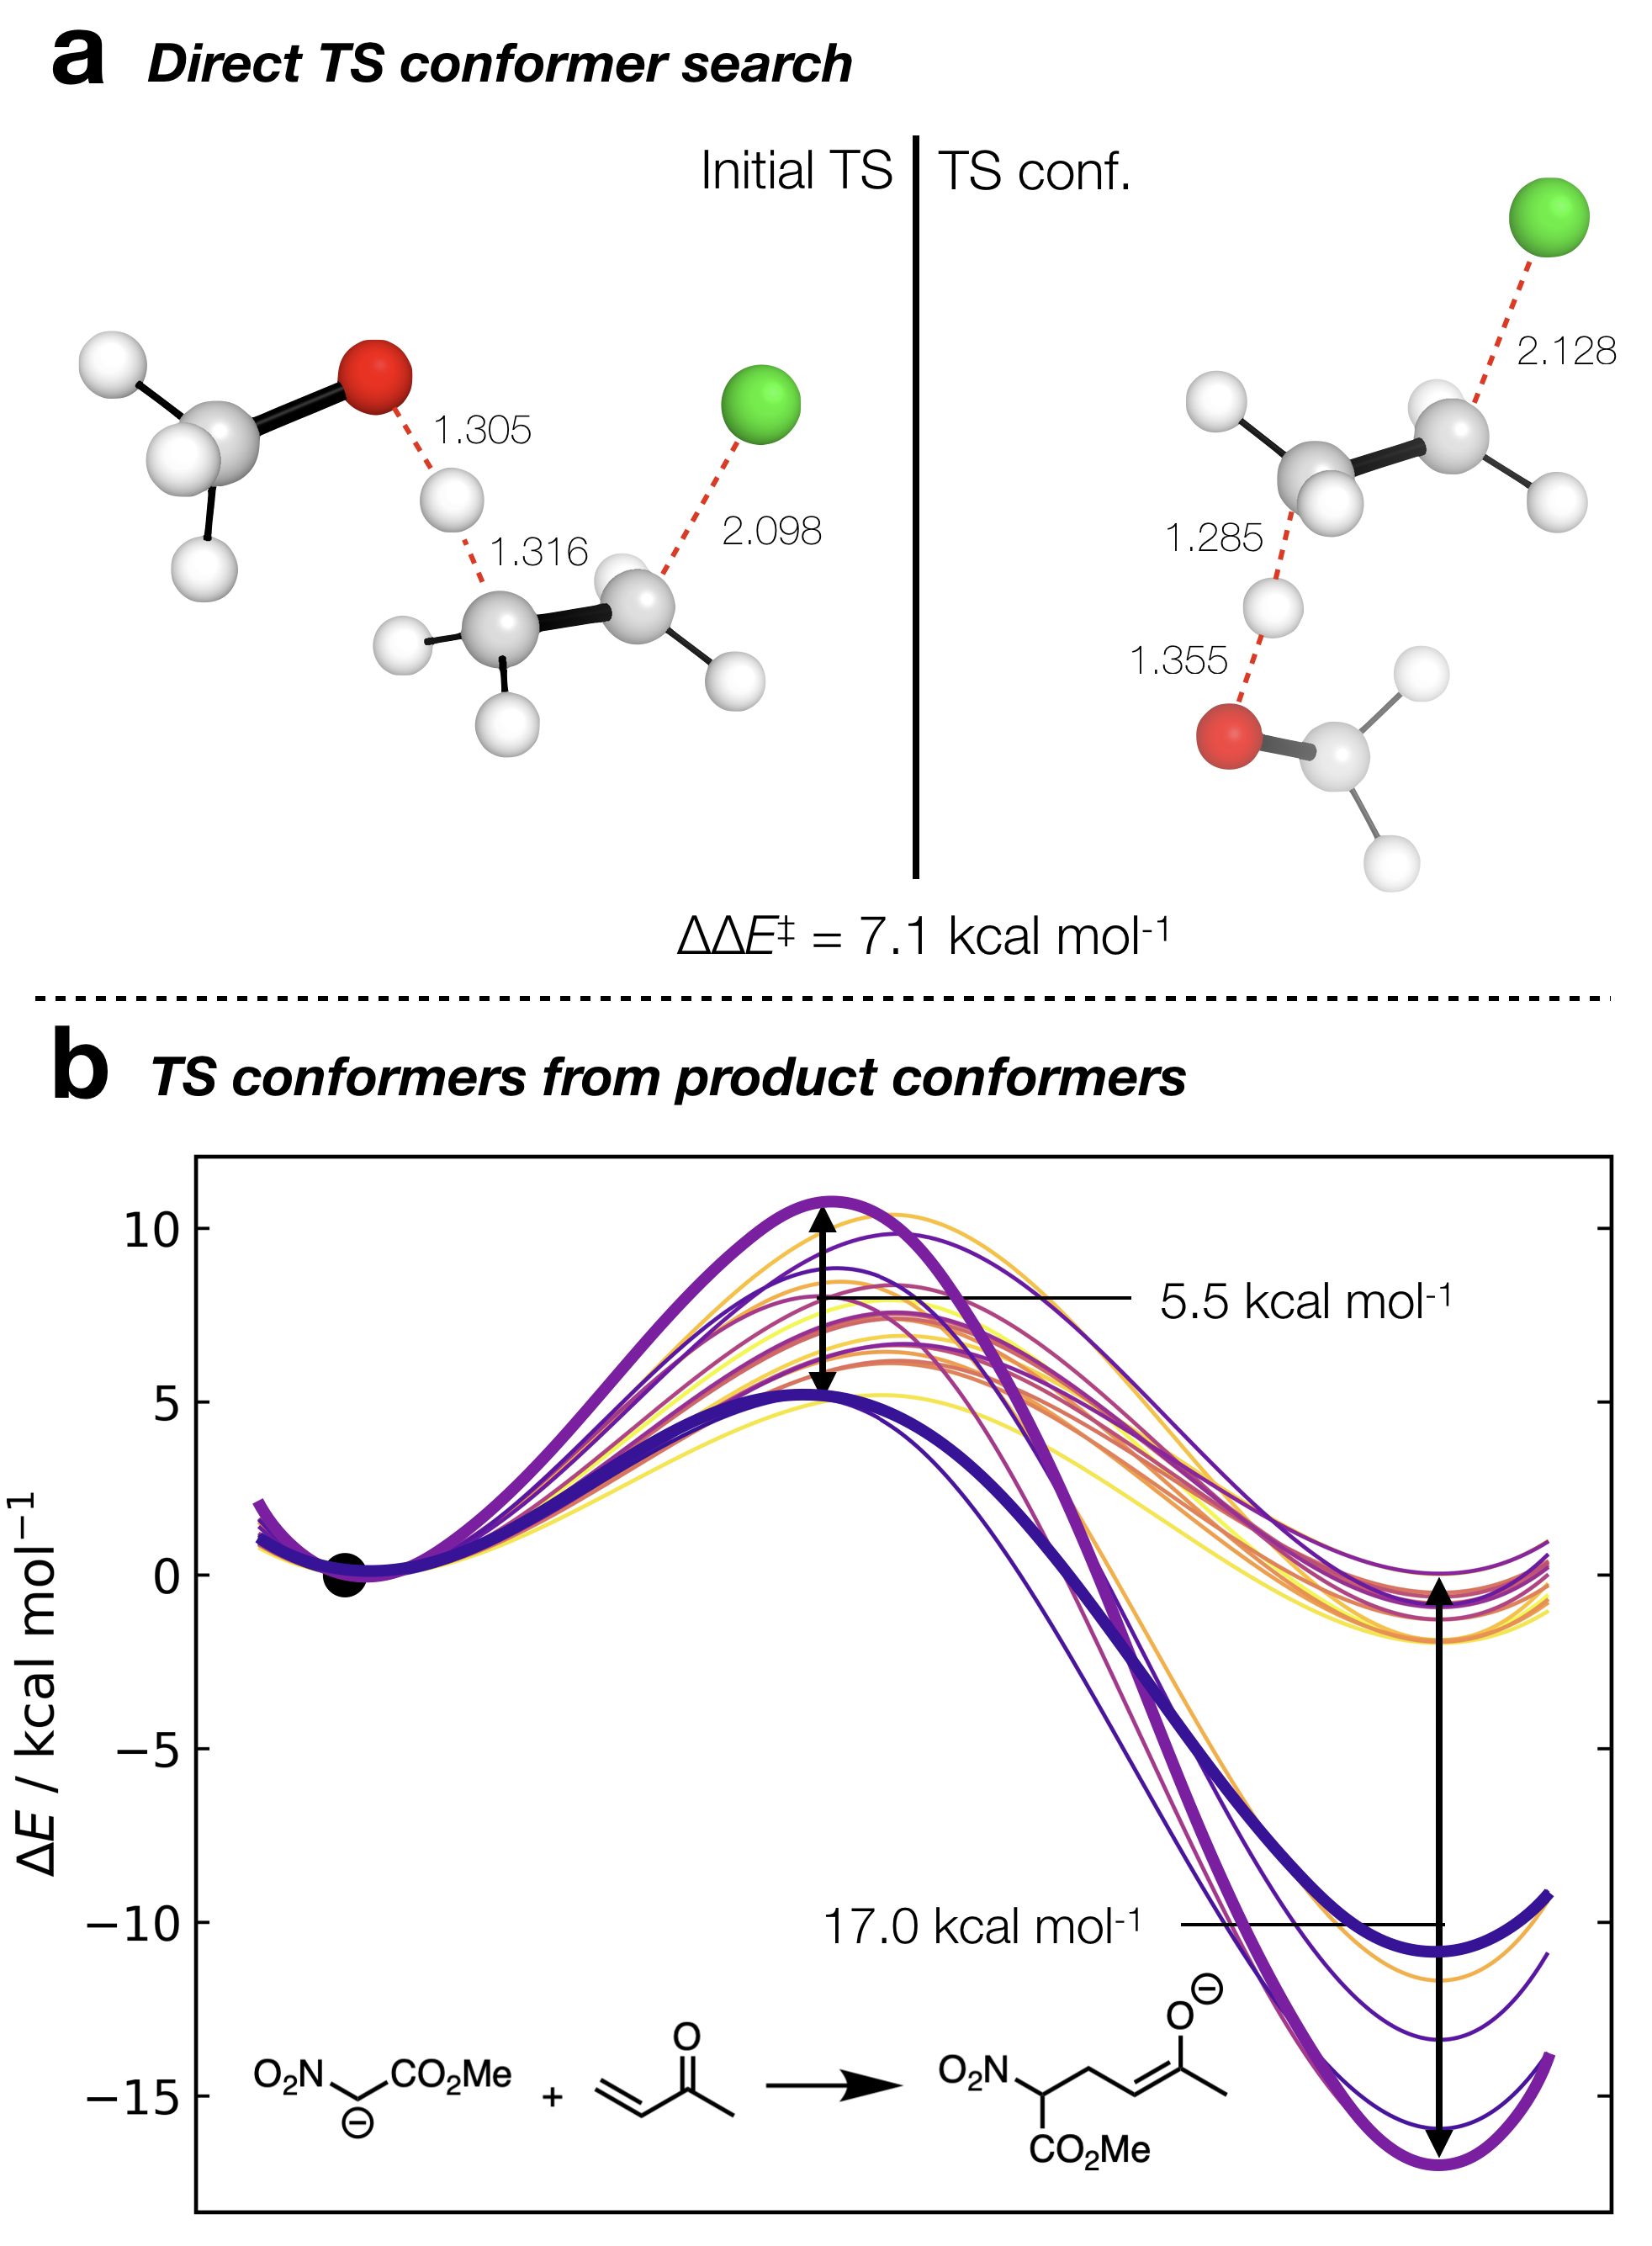
\includegraphics[width=10cm]{5/autode/figs/fig6}
	\vspace{0.4cm}
	\hrule
	\caption{(a) Lowest energy transition state conformers found with \ade for methoxide + chloroethane E2 elimination. (b) TS and product conformer distributions for the addition reaction between nitromethyl acetate and methyl vinyl ketone. Calculations performed at the CPCM(H$_2$O)-PBE0-D3BJ/ma-def2-SVP level of theory and distances quoted in \AA.}
	\label{fig::ade_6}
\end{figure}


{\bfseries{Organic Reaction}}. For \ade to become routinely used in mechanistic investigations, it must be applicable to synthetically relevant, and usually more complex, reactions. Here, we considered the Ireland--Claisen rearrangement explored computationally via trial-and-error and the AFIR method.\cite{Lee2019} With known intermediates, processed as SMILES strings from Chemdraw\texttrademark, \ade was tested and compared to the human-guided approach, which originally involved the testing of various conceivable mechanisms. \ade delivered an essentially identical reaction profile and reduced the time from the year of reported human and compute effort (that included searching other possible pathways) to a few minutes of setup time and $\sim$600 CPUh (one day of computer time on 24 cores, Figure \ref{fig::ade_7}). Interestingly, \ade deviates $< 2$ \kcalx from the trial and error-based search (blue), with INT3 showing a larger difference of 5 \kcal, due to \ade finding a more stable intermediate than the one located previously.

This example demonstrates that a combination of chemical knowledge, required to hypothesize reasonable mechanisms, and the use of \emph{autodE}, can substantially speed up joint experimental and computational efforts to elucidate complex reaction mechanisms, and in this way advance the optimization of synthetic routes and the design of novel catalysts.


\begin{sidewaysfigure}
	
	\vspace{0.2cm}
	\centering
	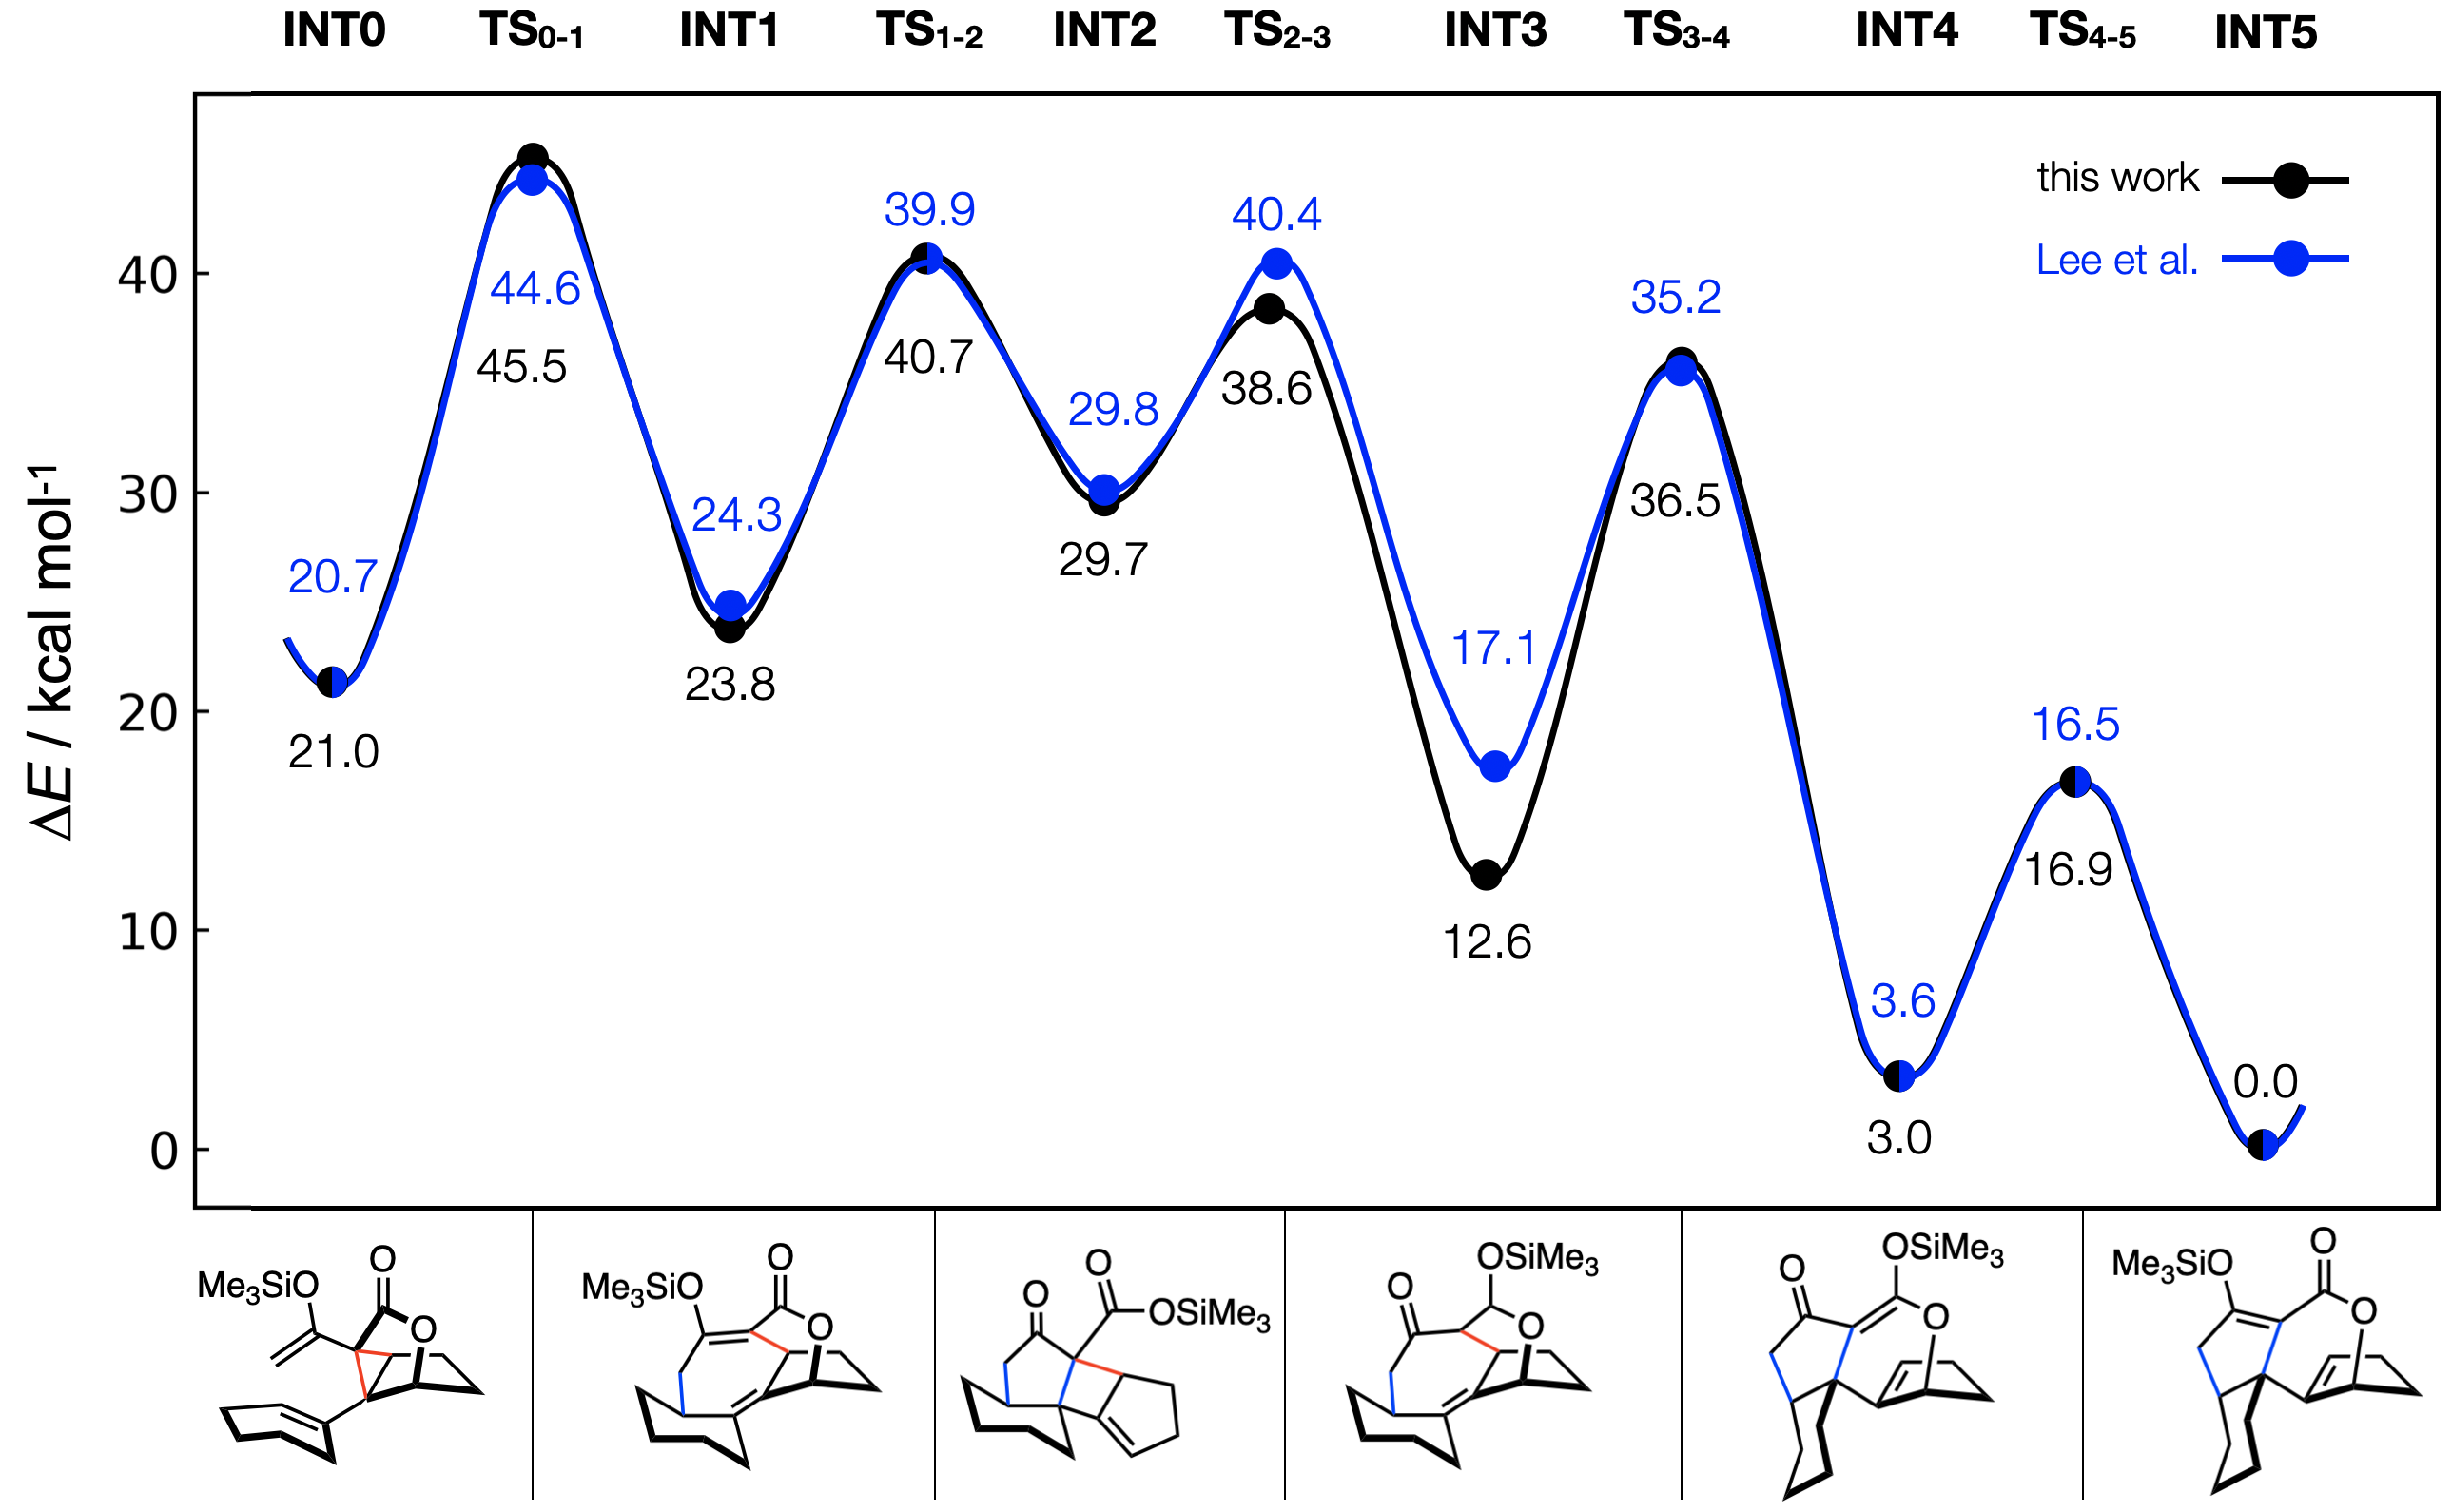
\includegraphics[width=0.75\textwidth]{5/autode/figs/fig7}
	\vspace{0.2cm}
	\hrule
	\caption{Ireland--Claisen rearrangement calculated using \ade (black) and described in ref. \cite{Lee2019} (blue) calculated at B3LYP-D3BJ/6-311++G(2d,2p)//B3LYP-D3BJ/6-31G(d). CPCM(hexane) solvent model used in ORCA (this work) and IEF-PCM(hexane) in Gaussian09 (from ref. \cite{Lee2019}). 3D Structures of the most stable intermediates and transition states are shown in Figure \ref{fig::ade_si_14}.}
	\label{fig::ade_7}
	
\end{sidewaysfigure}

{\bfseries{Organometallic Reaction}}. The conversion of alkenes into aldehydes via addition of CO and H$_2$ is an exceptionally important industrial process, making catalyst optimization the subject of considerable study.\cite{Franke2012} The general mechanism was discovered by Heck and Breslow\cite{Heck1961} and has been the subject of numerous computational studies (for an overview of these studies see ref. \cite{Kegl2015} and references cited therein). Those works have provided significant insights into the mechanism of the reaction, and highlighted the challenges associated with it. In fact, only finding the intermediates and transition states along the PES is already a laborious process, requiring extensive sampling, due to the presence of several conformers and isomeric forms (Figure \ref{fig::ade_8}a).

Applying \ade to study this catalytic cycle, using only the SMILES strings of the catalyst, ethylene, intermediates and products, the full reaction profile was obtained in less than 26 hours (16 CPU cores, excluding electronically barrierless ligand association steps, Figure \ref{fig::ade_8}b). \ade correctly identifies the most stable isomer of all intermediates; for example, the axial isomer for strong $\sigma$-donors (H: INT1, alkyl: INT3, acyl: INT5). TSs for all steps in the cycle are located successfully, i.e. they contain a single imaginary frequency and have geometries very similar to those found for analogous phosphine-based catalysts (Figure \ref{fig::ade_si_15}).\cite{Decker2001}


\begin{sidewaysfigure}
	
	\vspace{0.2cm}
	\centering
	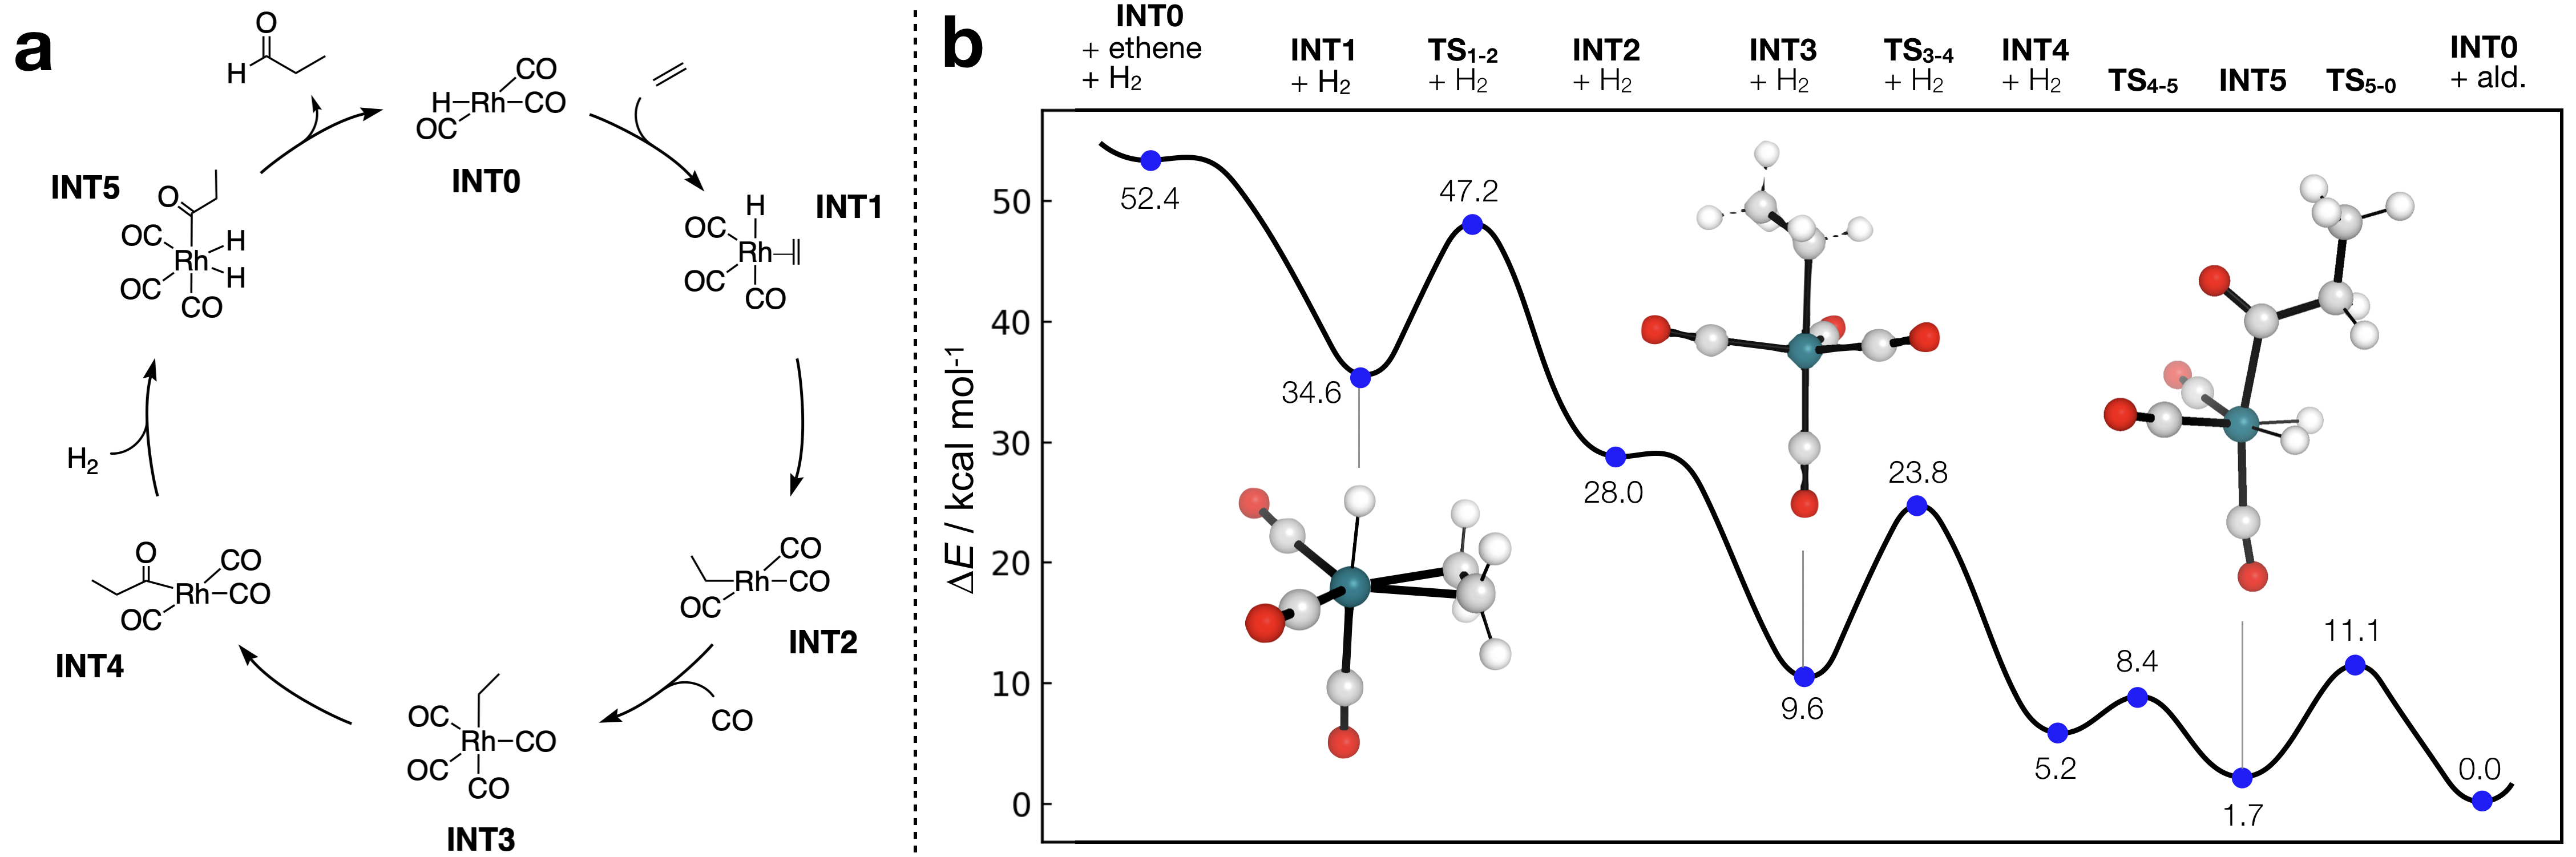
\includegraphics[width=\textwidth]{5/autode/figs/fig8}
	\vspace{0.2cm}
	\hrule
	\caption{(a) Heck-Breslow mechanism of hydroformylation in the absence of a phosphine catalyst. (b) Reaction profile calculated at PBE0-D3BJ/def2-TZVP//PBE0-D3BJ/def2-SVP in autodE.}
	\label{fig::ade_8}
	
\end{sidewaysfigure}

The same process was applied to the analogous Co-catalysed hydroformylation (Figure \ref{fig::ade_si_16}), which has been used as a representative example in other automated reaction generation algorithms.\cite{Kim2018, Habershon2016, Maeda2012} Once again, all TSs were successfully located with minutes of setup time. 

With a view to expand the use of \ade for catalyst design campaigns, and following previous efforts in this field,\cite{Guan2018} we have also developed the \emph{molfunc} tool \\
({\url{https://github.com/duartegroup/molfunc}}). Combining \ade with \emph{molfunc} enables a rapid screening of different catalysts by performing functionalisation of hydrogenic or other monovalent atomic positions. For example, for the H-insertion step, \emph{molfunc} facilitates the automated exploration of different groups at the para position of triphenyl phosphine on the barrier (Figure \ref{fig::ade_si_17}). The obtained positive correlation between the enhanced electron withdrawing ability of the catalyst and rate agrees with the experimental observation.\cite{Kegl2015} 


{\bfseries{Further Examples}}. To demonstrate the generality of our method, we tested \ade on a set of 15 simple organic reactions of different classes. \ade finds all TSs in all cases and generates reactions profiles in a matter of hours (Figure \ref{fig::ade_si_18a}). Further examples include metal-catalysed carbonylation of methanol to generate acetic acid via the Monsanto and Cativa processes (see full SI),\cite{Jones2000} alkaline ester hydrolysis (Figure \ref{fig::ade_si_9}), a Houk-List TS (Figure \ref{fig::ade_si_23}),\cite{Armstrong2014} and 57 carbene insertion reactions reported in ref. \cite{Mieusset2008} (see full SI). In this latter case \ade correctly locates 55/57 insertion TSs, with two failures occurring when a QRC+graph isomorphism check fails to confirm the TS as linking reactants and products, despite the TS being correct. Moreover, TSs for synthetically relevant reactions including a key Diels-Alder step in a total synthesis of Brevianamide A investigated by Domingo et al.\cite{Domingo1997} and a diastereoselective epoxidation\cite{Schneebeli2009} are presented in the full SI.\footnote{Examples presented in the full SI were performed by Joseph J. Silcock.}


{\bfseries{Limitations}}. The graph-based approach affords two immediate limitations of the method: The need to define bonds, and checking stereochemistry. While bonds are generally well-defined in organic systems, they are not a rigid concept. This is partially alleviated by using not regenerating the molecular graphs from the 3D structure, rather than a molecular graph representation, and retaining the SMILES-defined connectivity but may afford an incorrect assignment of a ‘good’ TS, which actually does or does not lead to products/reactants. Furthermore, the isomorphism condition on reactants/products does not currently include a stereochemistry check – the algorithm simply finds the lowest energy TS. While this is often defined by the reaction type e.g., stereochemical inversion in S$_\text{N}$2 is generated by traversing the lowest energy TS, there are reactions where this is not adhered to. Furthermore, by enforcing a maximum connectivity change of four (up to 2 bonds breaking and forming) means that, for example, the TS in a synchronous Fritsch–Buttenberg–Wiechell rearrangement mechanism cannot be found. In this case, human intervention is necessary to prevent the very slow enumeration of $\sim 10$ 2D PES scans. Finally, we note a limitation in the current \lmethodx electronic structure theory methods used to generate conformers of reactant and product complexes. Reactions involving anions are particularly problematic, as at the GFN2-XTB level they are generally not sufficiently stable (even in implicit solvent) such that the reaction may be barrierless at the \lmethodx level. We hope that as semi-empirical/TB electronic structure methods become more accurate and/or DFT and WF methods become faster, this limitation will be mitigated. Because \ade does not rely on one specific method implementing novel methods should be straightforward.

{\bfseries{Further Development}}. There are several opportunities to increase the accuracy and efficiency of \emph{autodE}, including (1) addition of explicit solvation; (2) inclusion of an online and open-source transition state library; (3) treatment of dynamical effects and (4) enhanced error correction. Initial progress has been made on explicit solvation using a simple QM/MM embedding scheme, but for the time being is too computationally demanding to routinely replace implicit solvation models. Future developments to the code will focus on these aspects to approach a fully automated protocol to predict reaction mechanisms with chemical accuracy.

\subsection{Conclusion}

Converting a 2D representation of a reaction to a reaction profile has long been the domain of expert computational chemists. Here we have shown that our method, \emph{autodE}, can largely automate this process and present a selection of both simple and synthetically interesting organic and organometallic reactions. By building a flexible framework in a way that does not rely on a particular electronic structure theory method, future methods for calculating points on the potential energy surface are easy to include. Indeed, the dominant source of failure of the methodology is due to inaccuracies in electronic structure methods rather than issues associated with \emph{autodE}. Crucially, \emph{autodE} is open source, making the development faster, more collaborative and more robust. We believe \emph{autodE} will facilitate faster computational investigation for both newcomers and experts alike.


\clearpage

\section{Selected Supporting Information III}
\emph{Full Supporting Information including raw data can be found at}:\\ {\url{https://onlinelibrary.wiley.com/doi/10.1002/anie.202011941}}


\subsection{Computational Methods}

All \ade calculations were performed with a development version of the code (1.0.0a0). Unless otherwise stated the \lmethodx used was GFN2-XTB v. 6.2\cite{Bannwarth2019} and the \hmethodx ORCA v. 4.2\cite{Neese2017} All ORCA optimizations employed resolution of identity DFT (RI or RIJCOSX for hybrid functionals)\cite{Neese2003, Neese2009} using the PBE\cite{Perdew1996} or PBE0\cite{Adamo1999} functional, in combination with the D3BJ dispersion correction,\cite{Grimme2010, Grimme2011} def2-SVP or def2-TZVP basis set\cite{Weigend2005} (with effective core potentials for Rh) and the default auxiliary basis set.\cite{Weigend2006} Gaussian09\cite{G09} calculations employed identical methods without density fitting unless otherwise specified. NWChem v. 6.6\cite{Valiev2010} calculations used no dispersion correction as D3BJ is unavailable with PBE0. Default integration grids were used in all DFT calculations. Conformers generated with RDKit\cite{Landrum2019} version 2020.03.1 and OpenBabel version 2.4.1.


\subsection{Compatibility of autodE with Different Electronic Structure Theory Codes}

Figure \ref{fig::ade_si_1a} shows the energy profile for the endo/exo Diels Alder cyclization between methyl acrylate and cyclopentadiene obtained when combining \ade with each of the software for which wrappers are currently implemented and show invariability of the results to the chosen method. 


\begin{figure}[h!]
	\vspace{0.4cm}
	\centering
	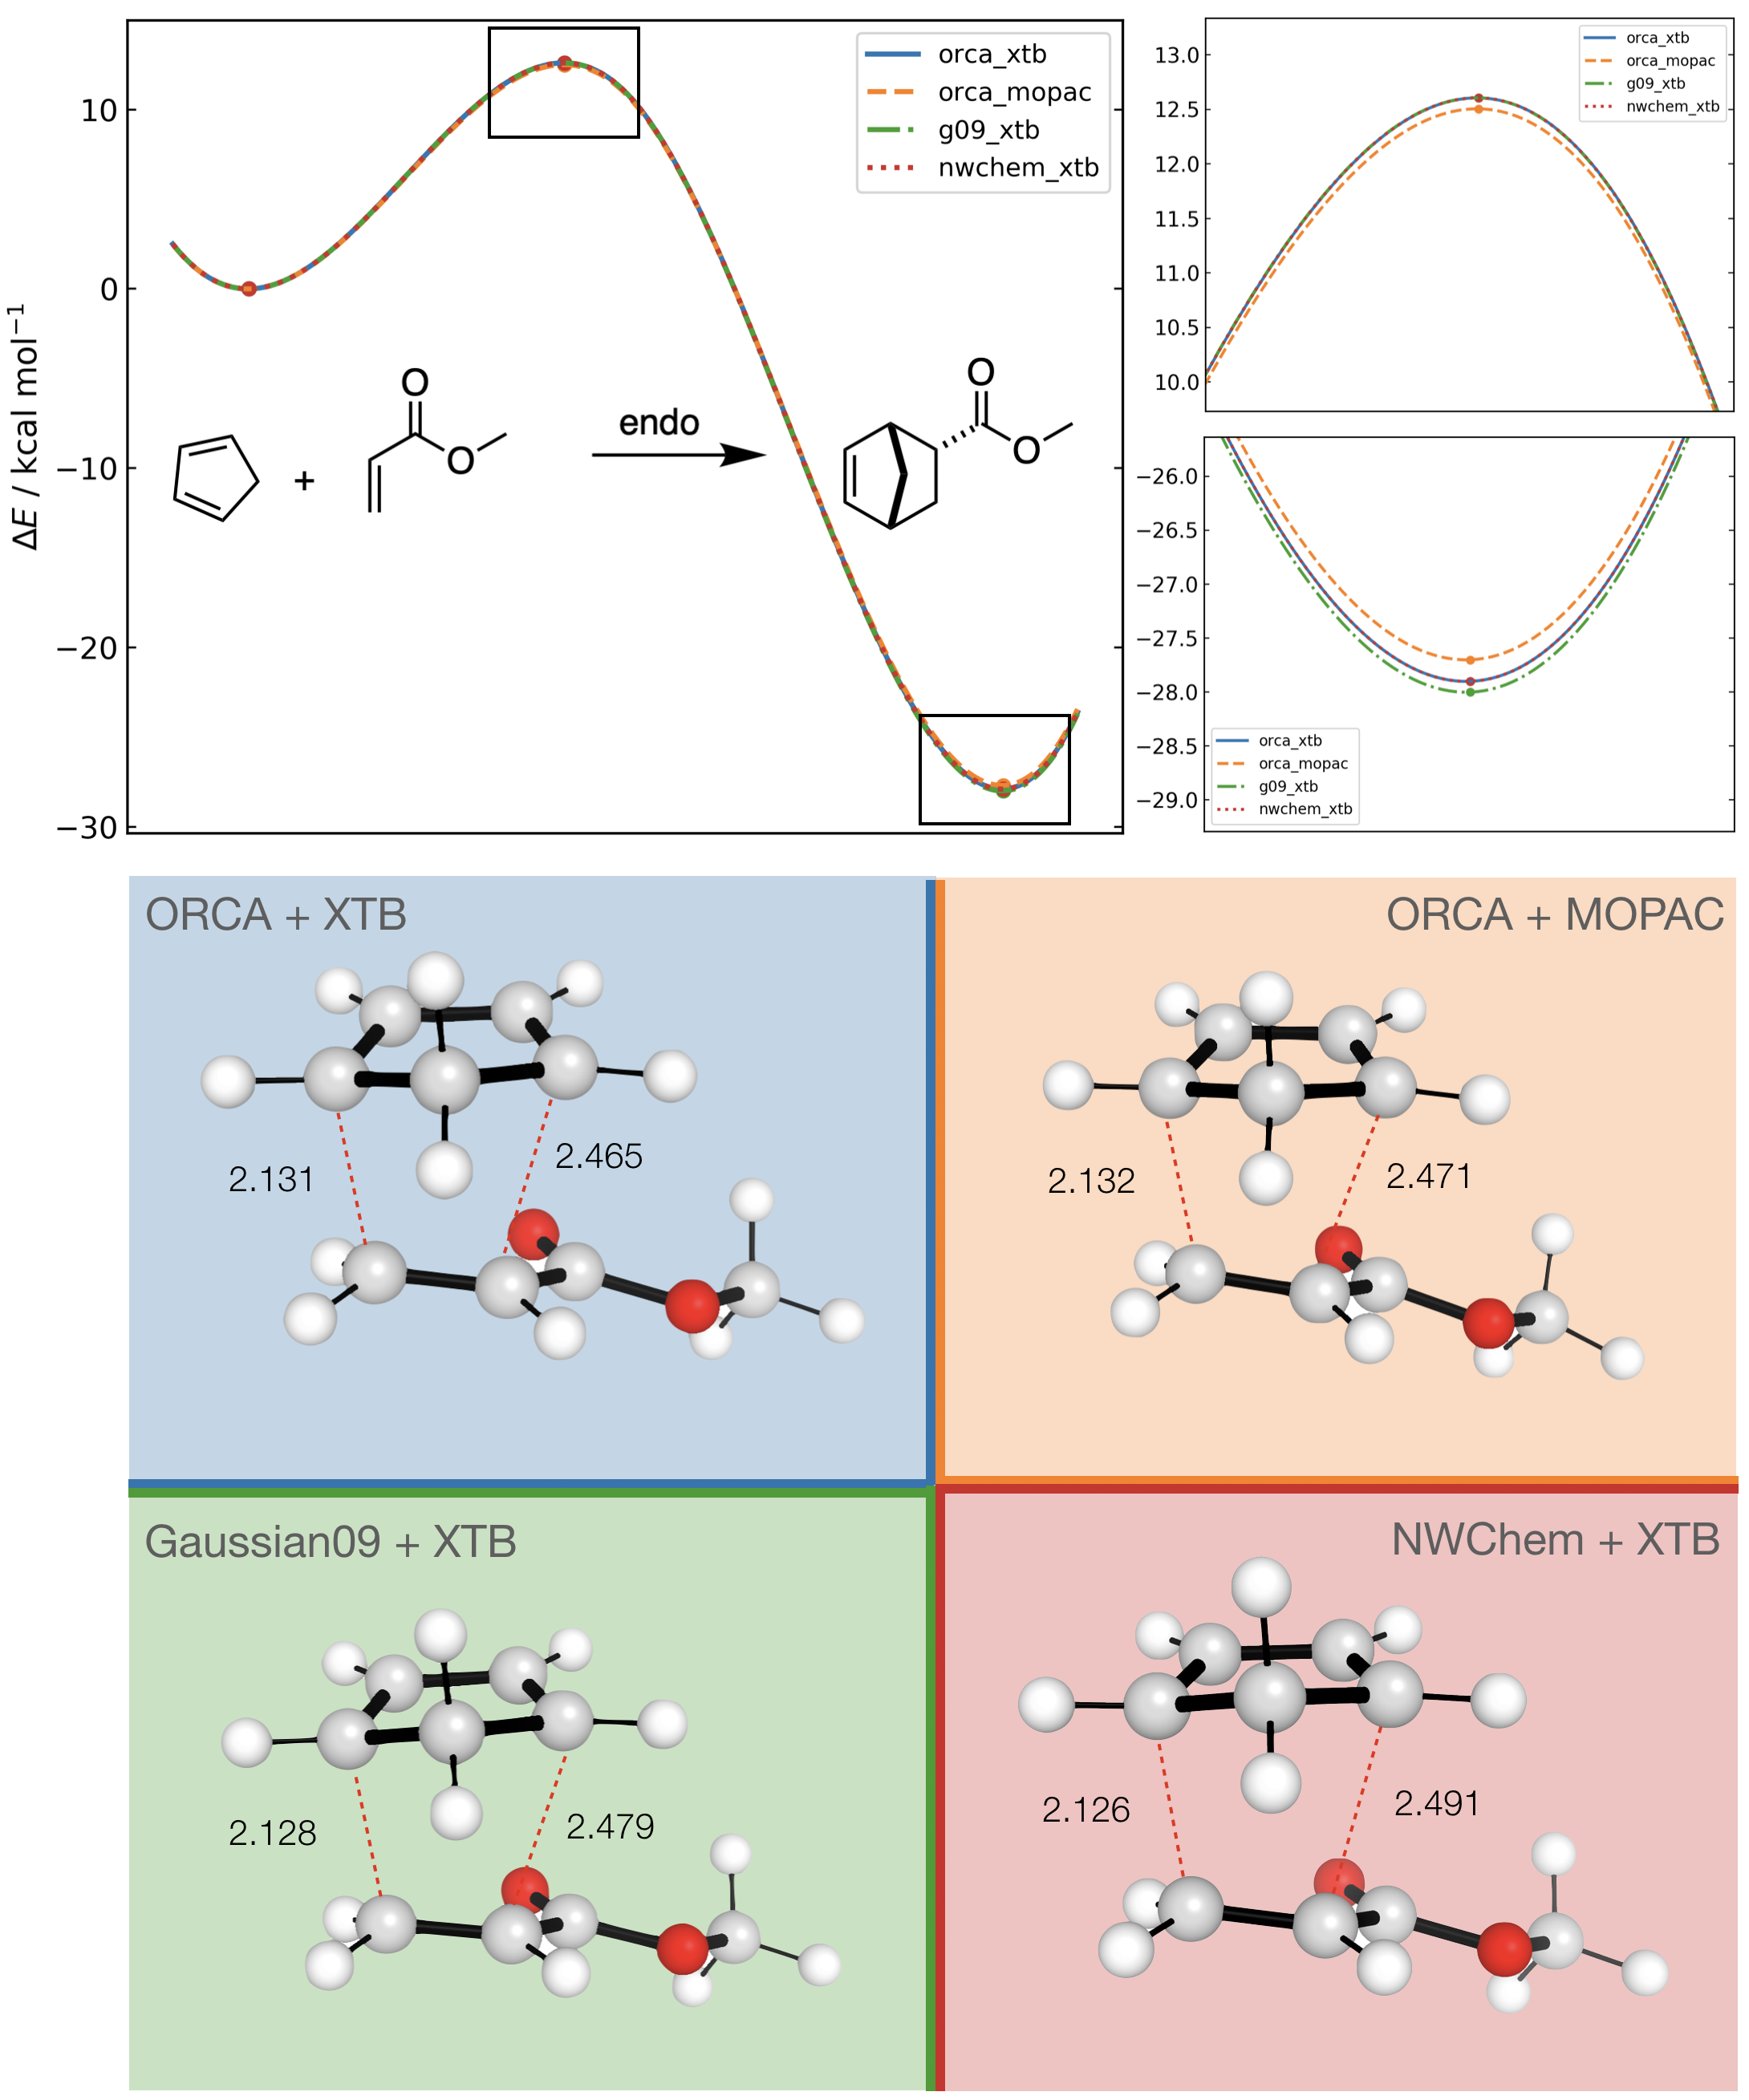
\includegraphics[width=14cm]{5/autode/figs/figS1a}
	\vspace{0.4cm}
	\hrule
	\caption{Comparison of different codes used to perform optimizations and single point energy evaluations in the reaction between \emph{endo} Diels--Alder cyclisation between methyl acrylate and cyclopentadiene. All profiles are calculated at the PBE0/def2-TZVP//PBE0/def2-SVP level of theory and the low-level method is tight-binding DFT (XTB) or semi-empirical PM7 (MOPAC). Forming bond distances are quoted in \AA.}
	\label{fig::ade_si_1a}
\end{figure}


\begin{figure}[h!]
	\vspace{0.4cm}
	\centering
	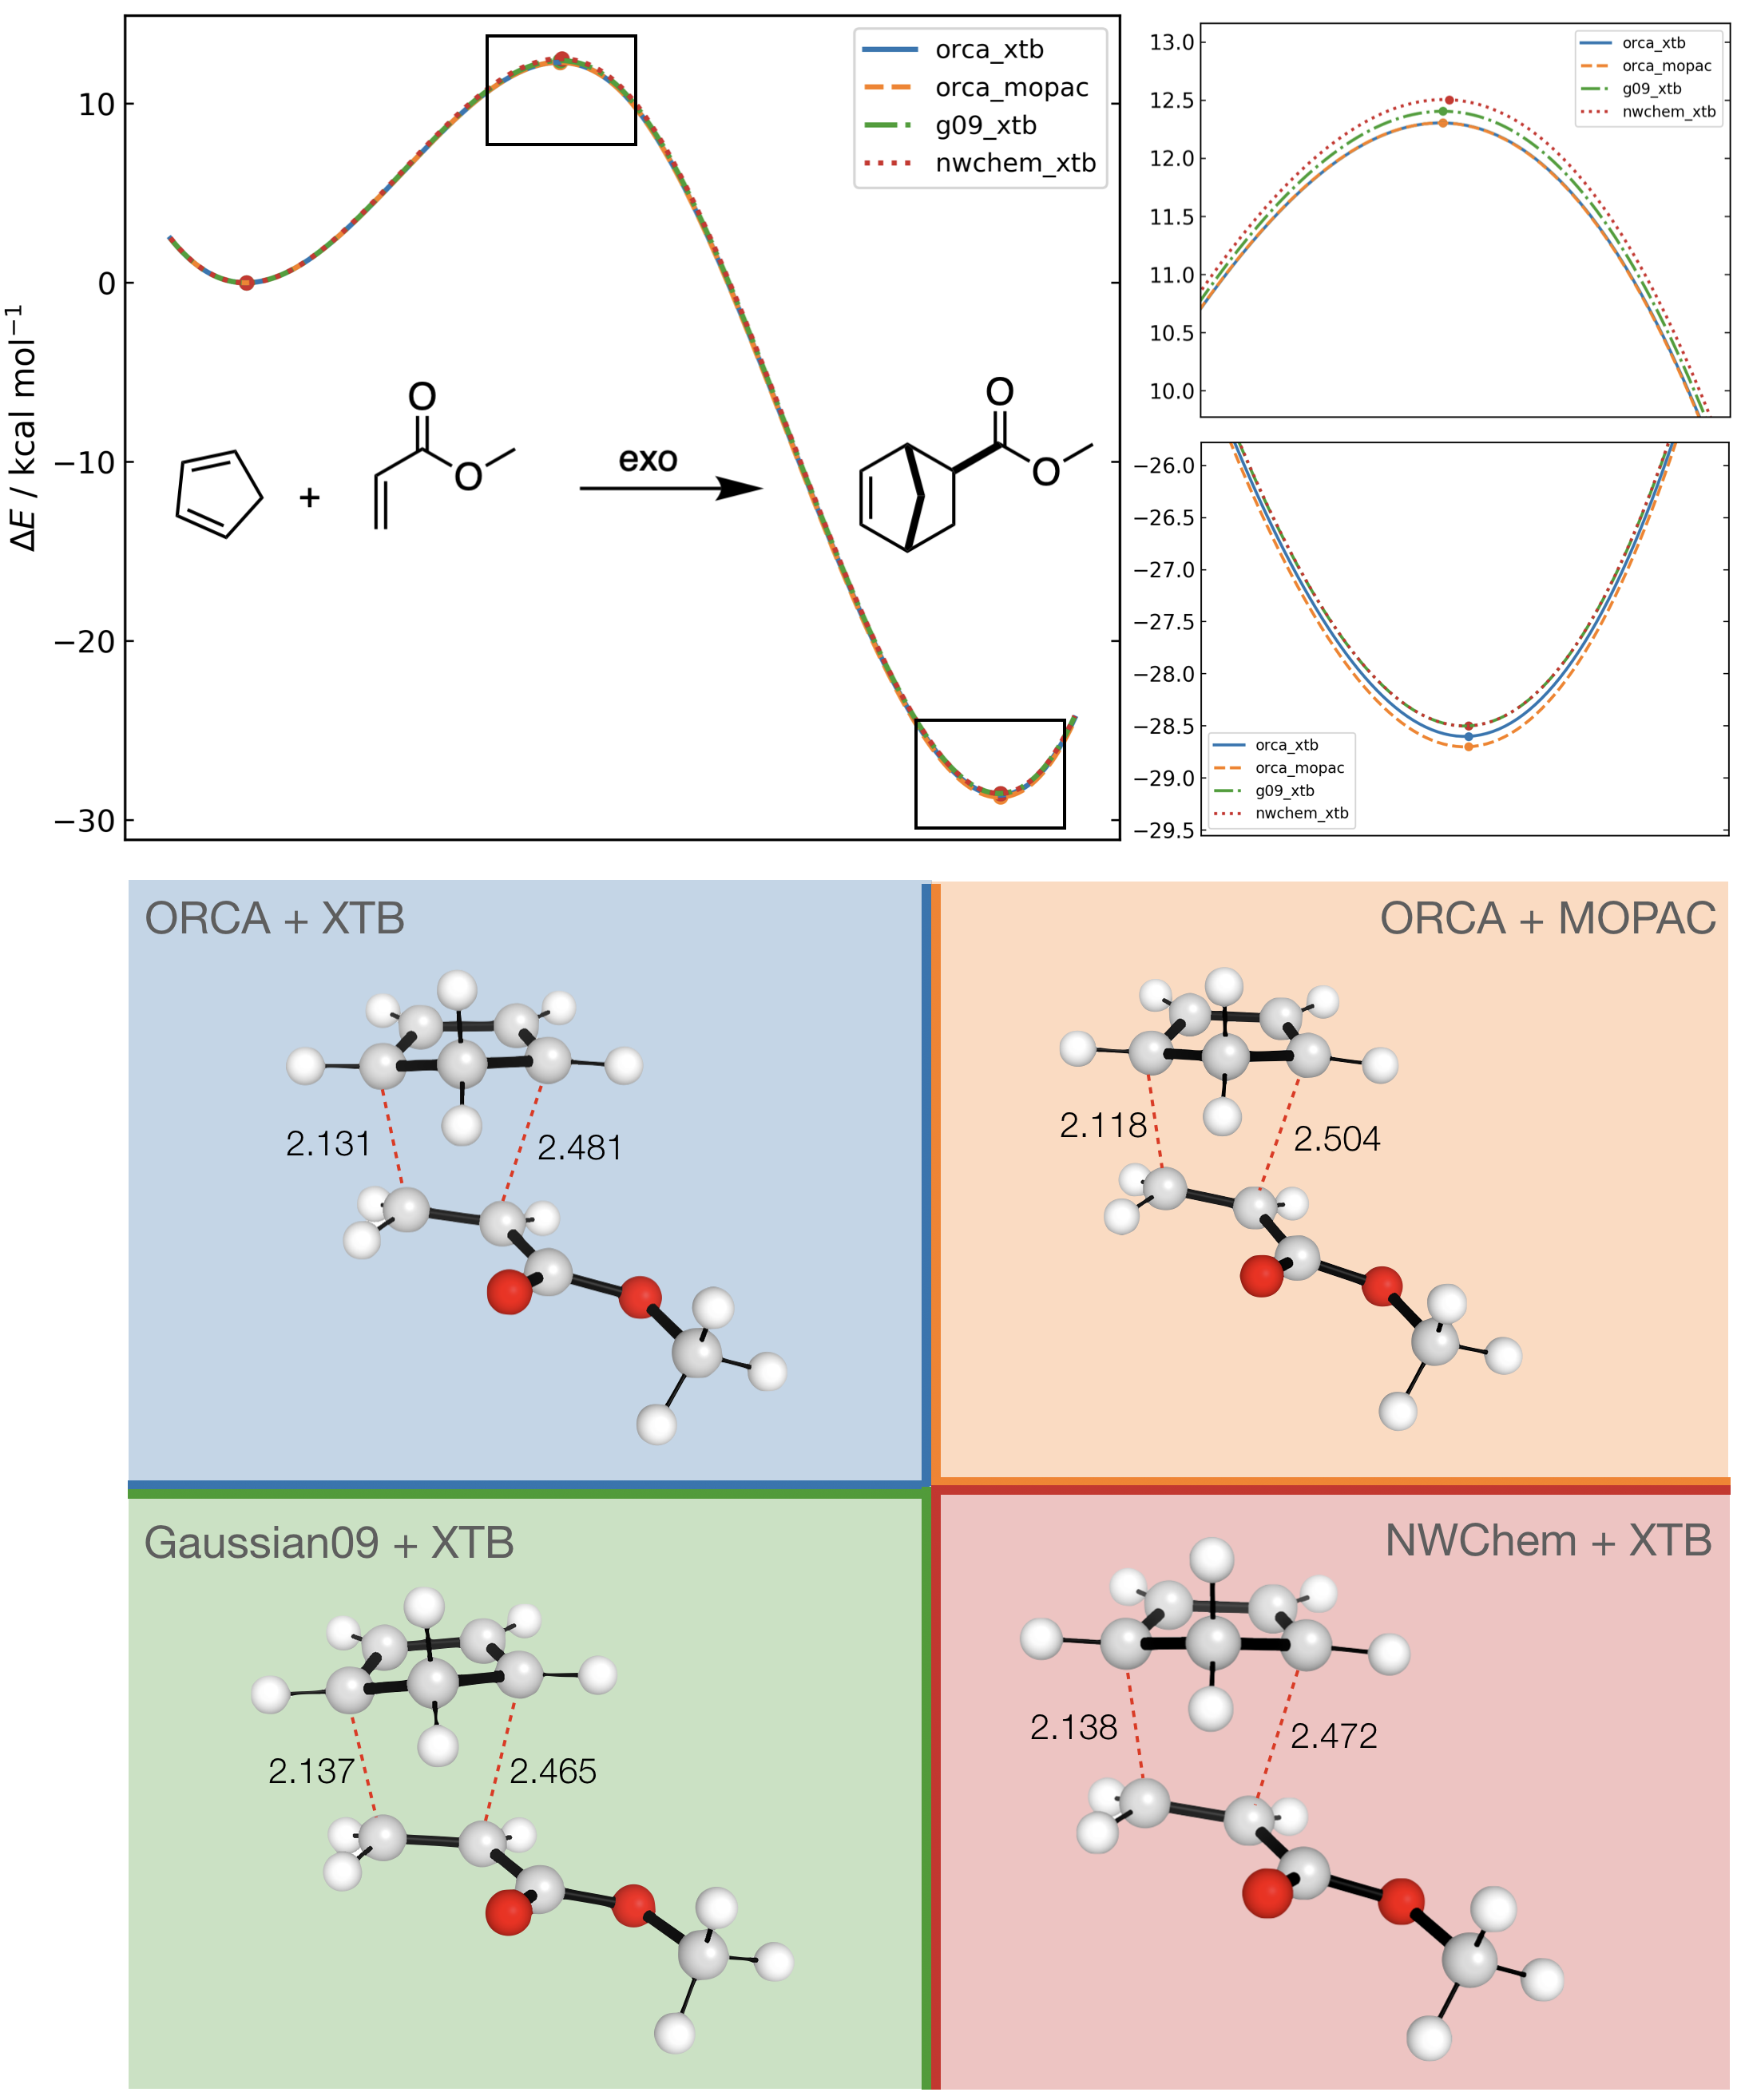
\includegraphics[width=14cm]{5/autode/figs/figS1b}
	\vspace{0.4cm}
	\hrule
	\caption{As Figure \ref{fig::ade_si_1a} for \emph{exo} products.}
	\label{fig::ade_si_1b}
\end{figure}



\begin{figure}[h!]
	\vspace{0.4cm}
	\centering
	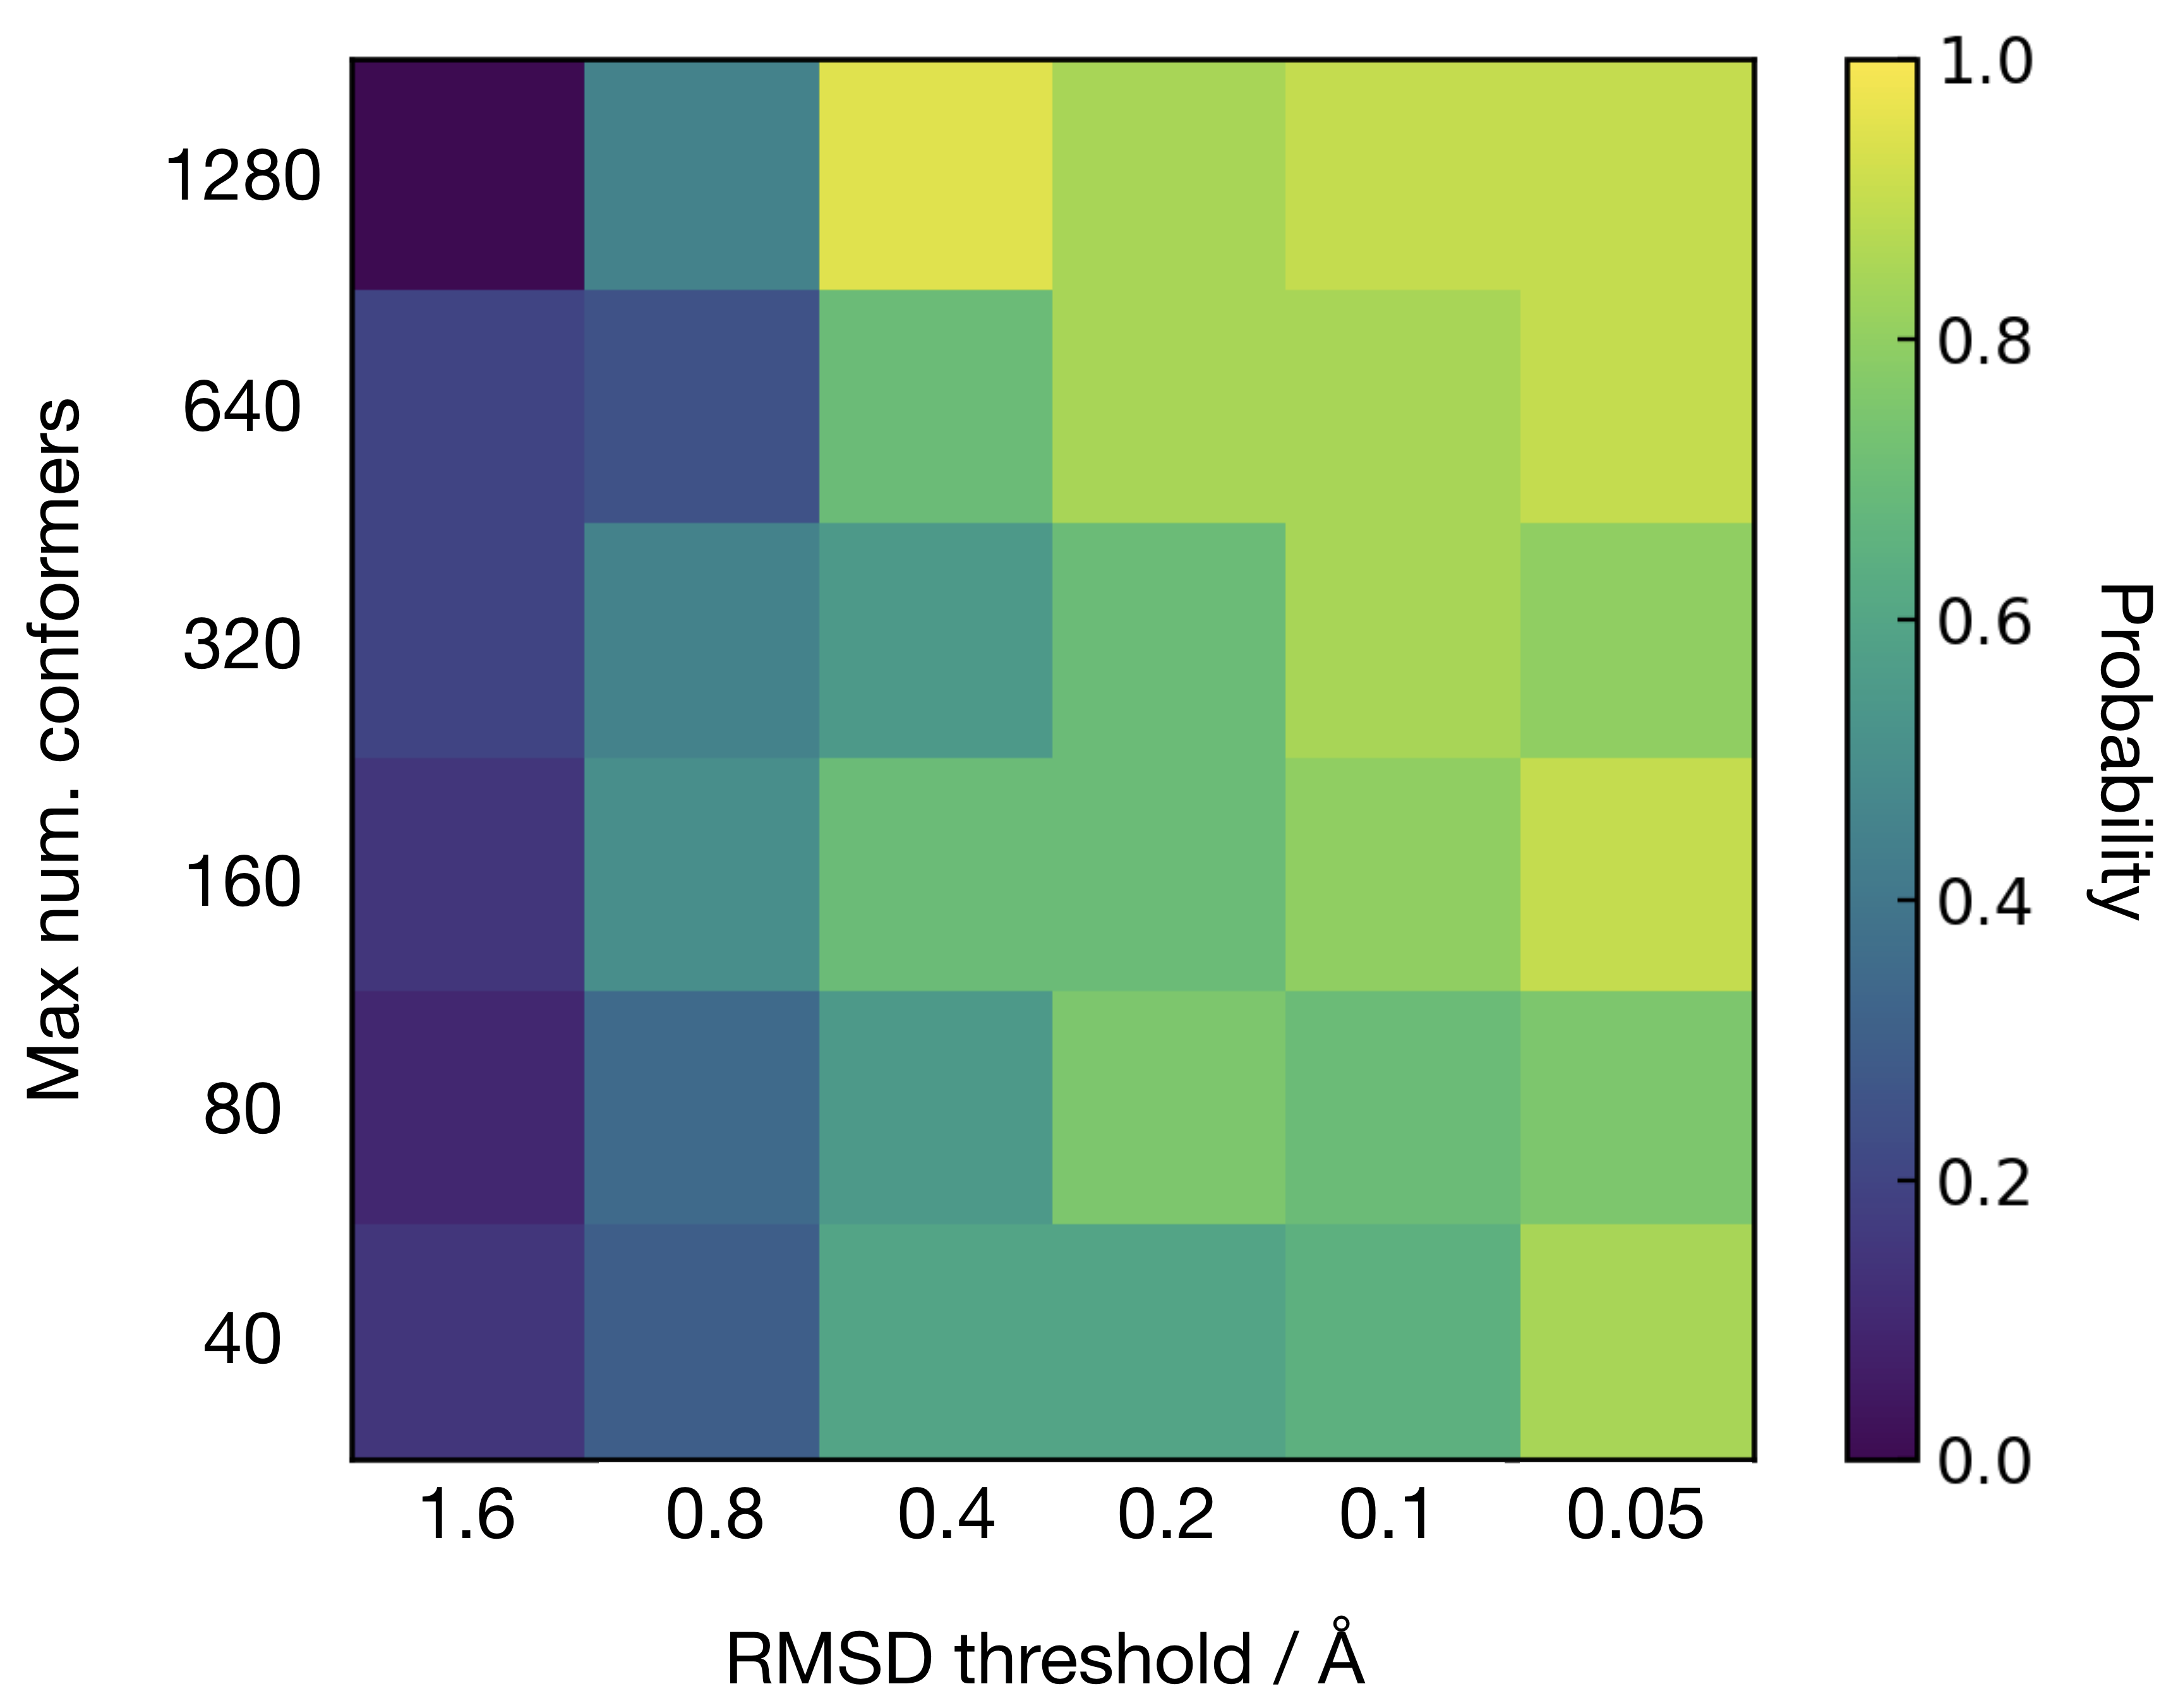
\includegraphics[width=11cm]{5/autode/figs/figS2}
	\vspace{0.4cm}
	\hrule
	\caption{Probability that a conformer will be found -- using RDKit + XTB optimization -- within 1 \kcalx of the most stable conformer generated by CREST given a specific root mean squared deviation (RMSD) and a number of conformers threshold in the EKTDGv2 algorithm. Molecule set contains 20 L-amino acids. All optimizations were performed at the GFN2-XTB level. Crest v. 2.9 \& XTB v. 6.2.3 to find the lowest energy conformer, as it generated a more diverse set than the exhaustive algorithm in CONFAB. For example, CREST generated 90 conformers for serine for which 85 were found in ref. \cite{He2016} while CONFAB did not identify the correct rotatable bonds and afforded only 36 conformers.}
	\label{fig::ade_si_2}
\end{figure}

\clearpage
\subsection{Metal-complex Conformers}
\label{section::ade_si_metal_complex_confs}

\ade generates metal complex conformers using Eqn. \eqref{equation::ade_1_repeat},


\begin{equation}
	U_\text{RB}(\boldsymbol{x}) = \sum_{ij \in \text{bonds}} k_1 (r_{ij} - r_{ij}^\text{avg})^2 + \sum_{i > j} \frac{k_2}{r_{ij}^n}
	\label{equation::ade_1_repeat}
\end{equation}


where the first harmonic term describes bonds between atoms, and the second term introduces a non-physical repulsion that enforces a notion of steric repulsion. Parameters $k_1 = 1$ and $k_2 = 0.01$ were selected based on empirical experience and comparison to optimised structures (Figure \ref{fig::ade_si_3}) while ideal bond lengths ($r^\text{avg}$) are obtained as averages from the Cambridge Structural Database.

To generate reasonable 3D structures for organometallic complexes, each atom is added sequentially and randomly in a 10 \AA$\;$ cubic box, and the function $U_\text{RB}$ is minimized with respect to all coordinates after each addition. Using a smooth potential with few local minima ($n = 2$ in Eqn. \eqref{equation::ade_1_repeat}) is required to obtain stable structures for large complexes (Figure \ref{fig::ade_si_4}). For a test set of 20 metal-complexes with up to 100 atoms, our approach delivers a stable conformer in all cases, while RDKit successfully generates only 15 geometries and CONFAB failed in all cases (Figure \ref{fig::ade_si_5a} and Table \ref{table::ade_si_1}). With the analytic derivative of $U_\text{RB}$ and a conjugate gradient algorithm implemented in \emph{scipy},\cite{SciPy} an initial structure is available in a few seconds for complexes with more than 100 atoms. Stereo-defined metal complexes are currently not supported, as random initialization does not respect any chirality.

An alternative and slightly faster approach is used to generate metal complex conformers; a random displacement vector (length $\sim3$ \AA) is applied to all atoms and $U_\text{RB}$ minimized with $n = 8$. The steeper repulsive term is used as it generates a more realistic PES; for example, generating the expected three minima in the butane dihedral PES, Figure \ref{fig::ade_si_4}. While simple, this strategy affords more conformers than both RDKit and CONFAB for the metal complex test set (Figure \ref{fig::ade_si_5a} and Table \ref{table::ade_si_1}). It is also worth noting that we found no advantage in using the EMBED algorithm\cite{Havel2002} to generate initial coordinates for organic systems (Figure \ref{fig::ade_si_6a}). Moreover, conformers can be generated using arbitrary distance constraints specified by the user (e.g., to retain a square planar geometry given an 3D initial structure).


\begin{figure}[h!]
	\vspace{0.4cm}
	\centering
	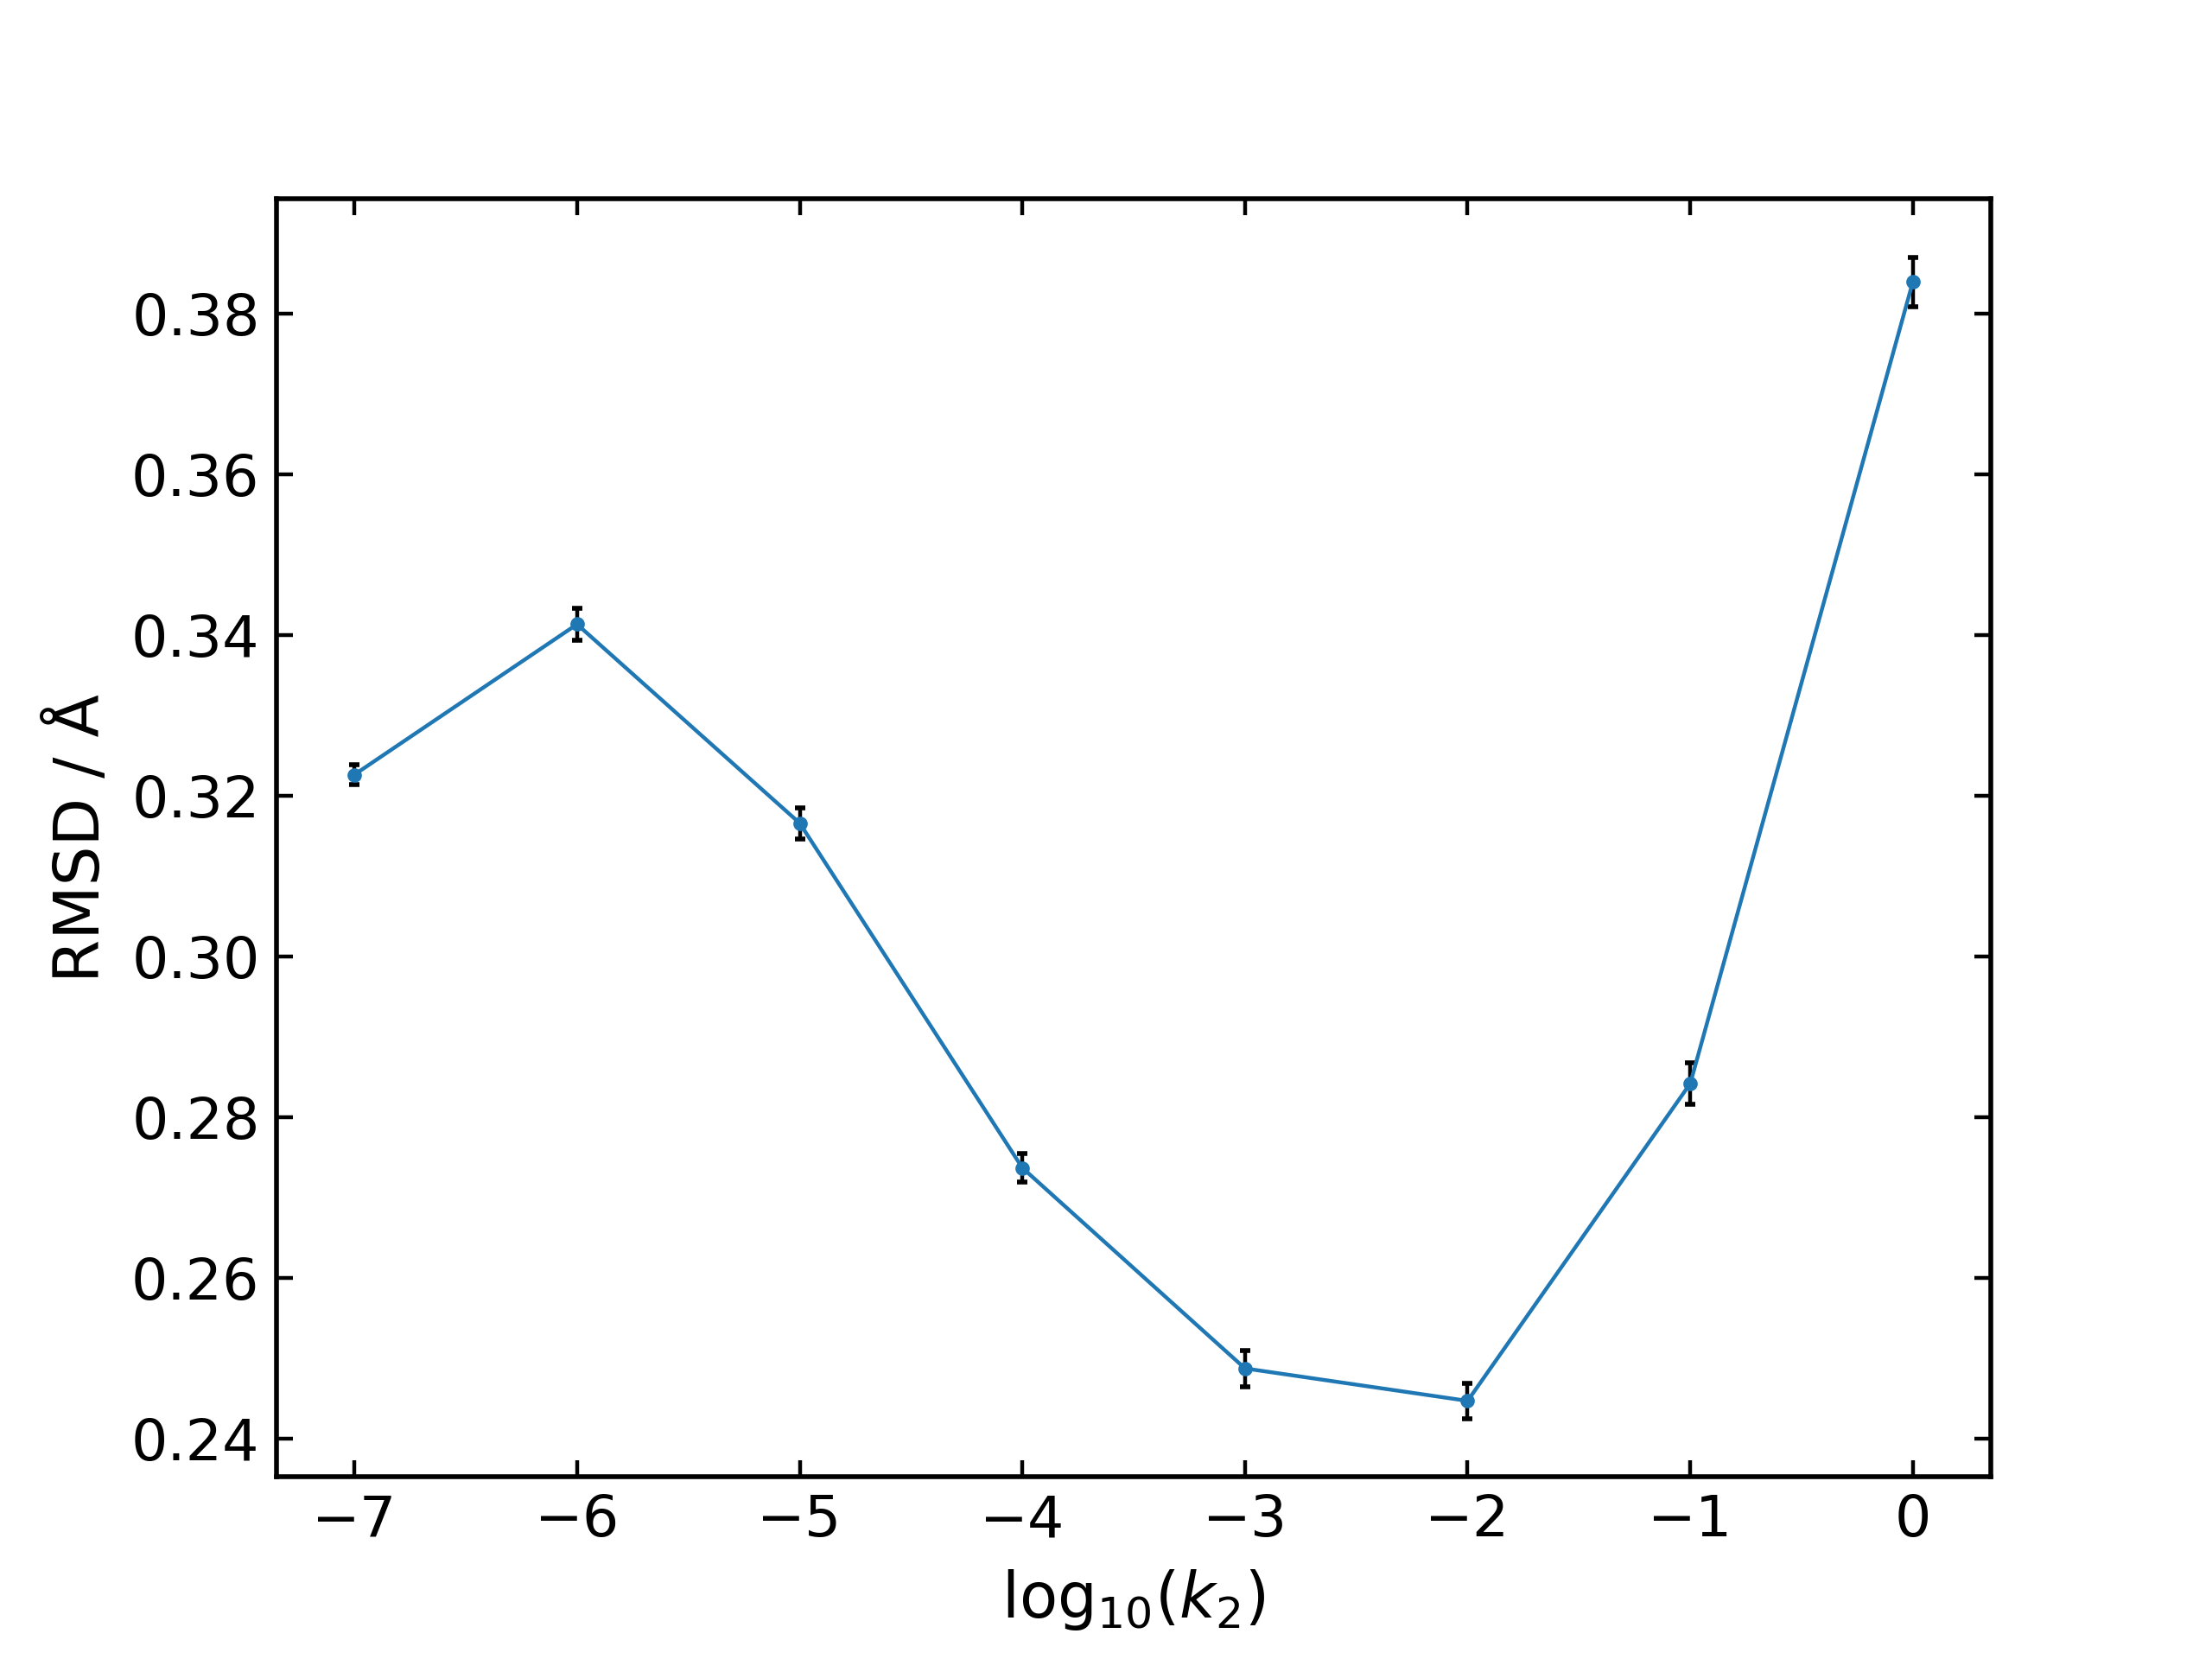
\includegraphics[width=11cm]{5/autode/figs/figS3}
	\vspace{0.4cm}
	\hrule
	\caption{Using the molecules butane, proline and [RhH(ethene)(CO)${}_3$], the calculated RMSD between the geometries optimised with the repulsion + bonded forcefield [\eqref{equation::ade_1_repeat} $n=8$] and XTB for different $k_2$ values (Eqn. \eqref{equation::ade_1_repeat}). Initial conformer geometries are obtained by random displacements from XTB-optimised geometries (normally distributed, $\sigma$=0.5 \AA, $\mu$=0.0 \AA, on each direction). This approach provides a more realistic starting structure than optimizing at the local XTB minimum i.e. not overly favouring a very small repulsion where atoms do not move from their optimised positions. Error bars are quoted as the standard error in the mean of 20 repeats.}
	\label{fig::ade_si_3}
\end{figure}



\begin{figure}[h!]
	\vspace{0.4cm}
	\centering
	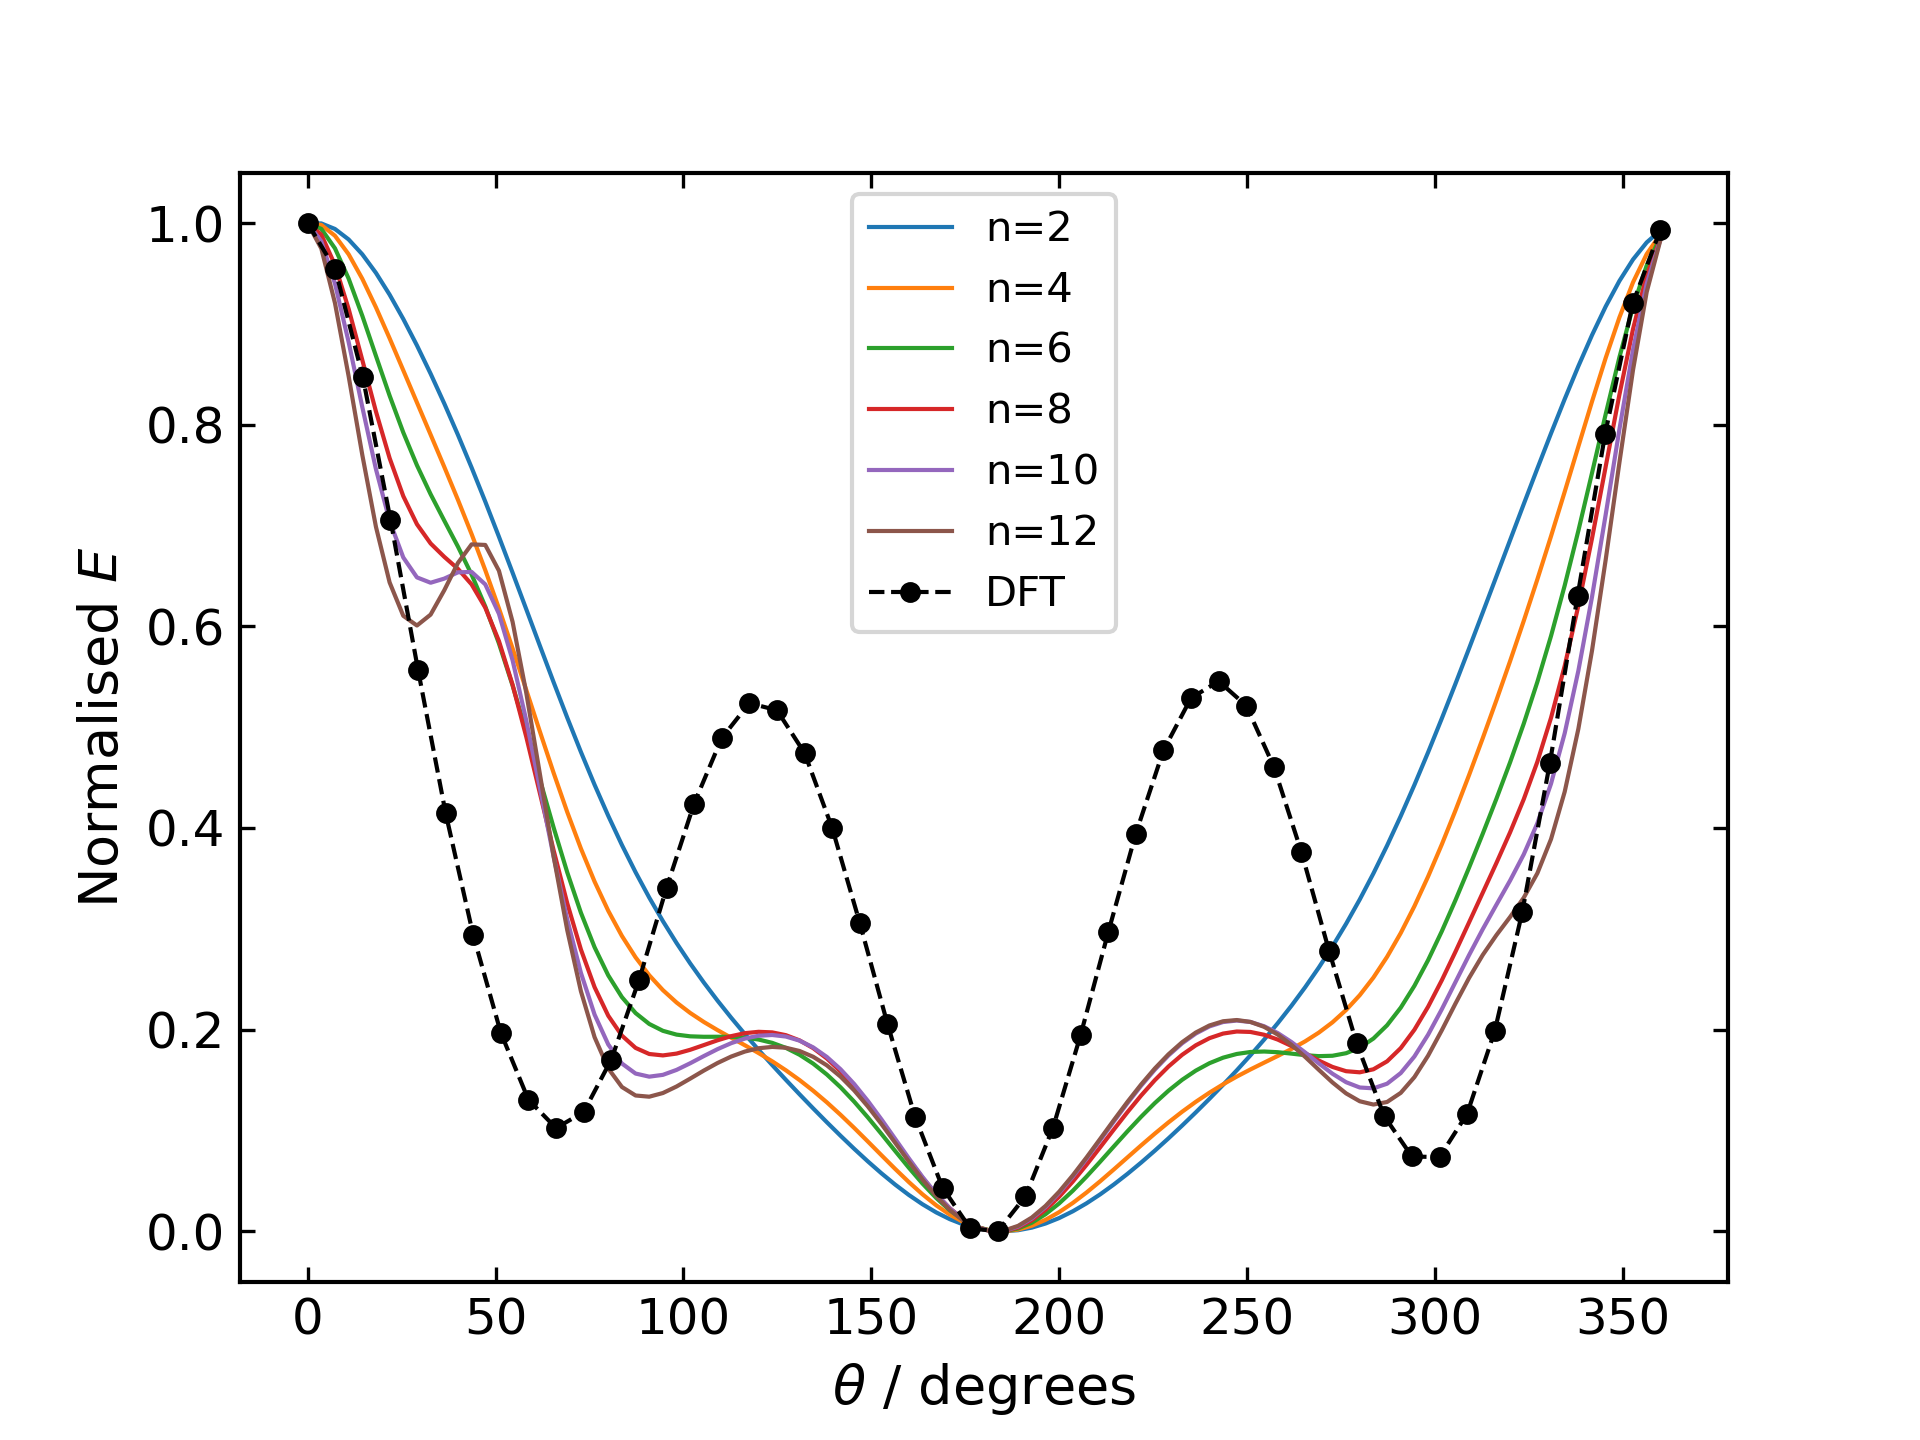
\includegraphics[width=12cm]{5/autode/figs/figS4}
	\vspace{0.4cm}
	\hrule
	\caption{Rotational barrier of butane using a simple repulsion + bonded potential Eqn. \ref{equation::ade_1_repeat}, with different n values, compared to a DFT reference (PBE0-D3BJ/def2-SVP). Relative energies normalized to the eclipsed conformation ($\theta$ = 0 $^{\circ}$). Initial structure not symmetrized.}
	\label{fig::ade_si_4}
\end{figure}



\begin{figure}[h!]
	\vspace{0.4cm}
	\centering
	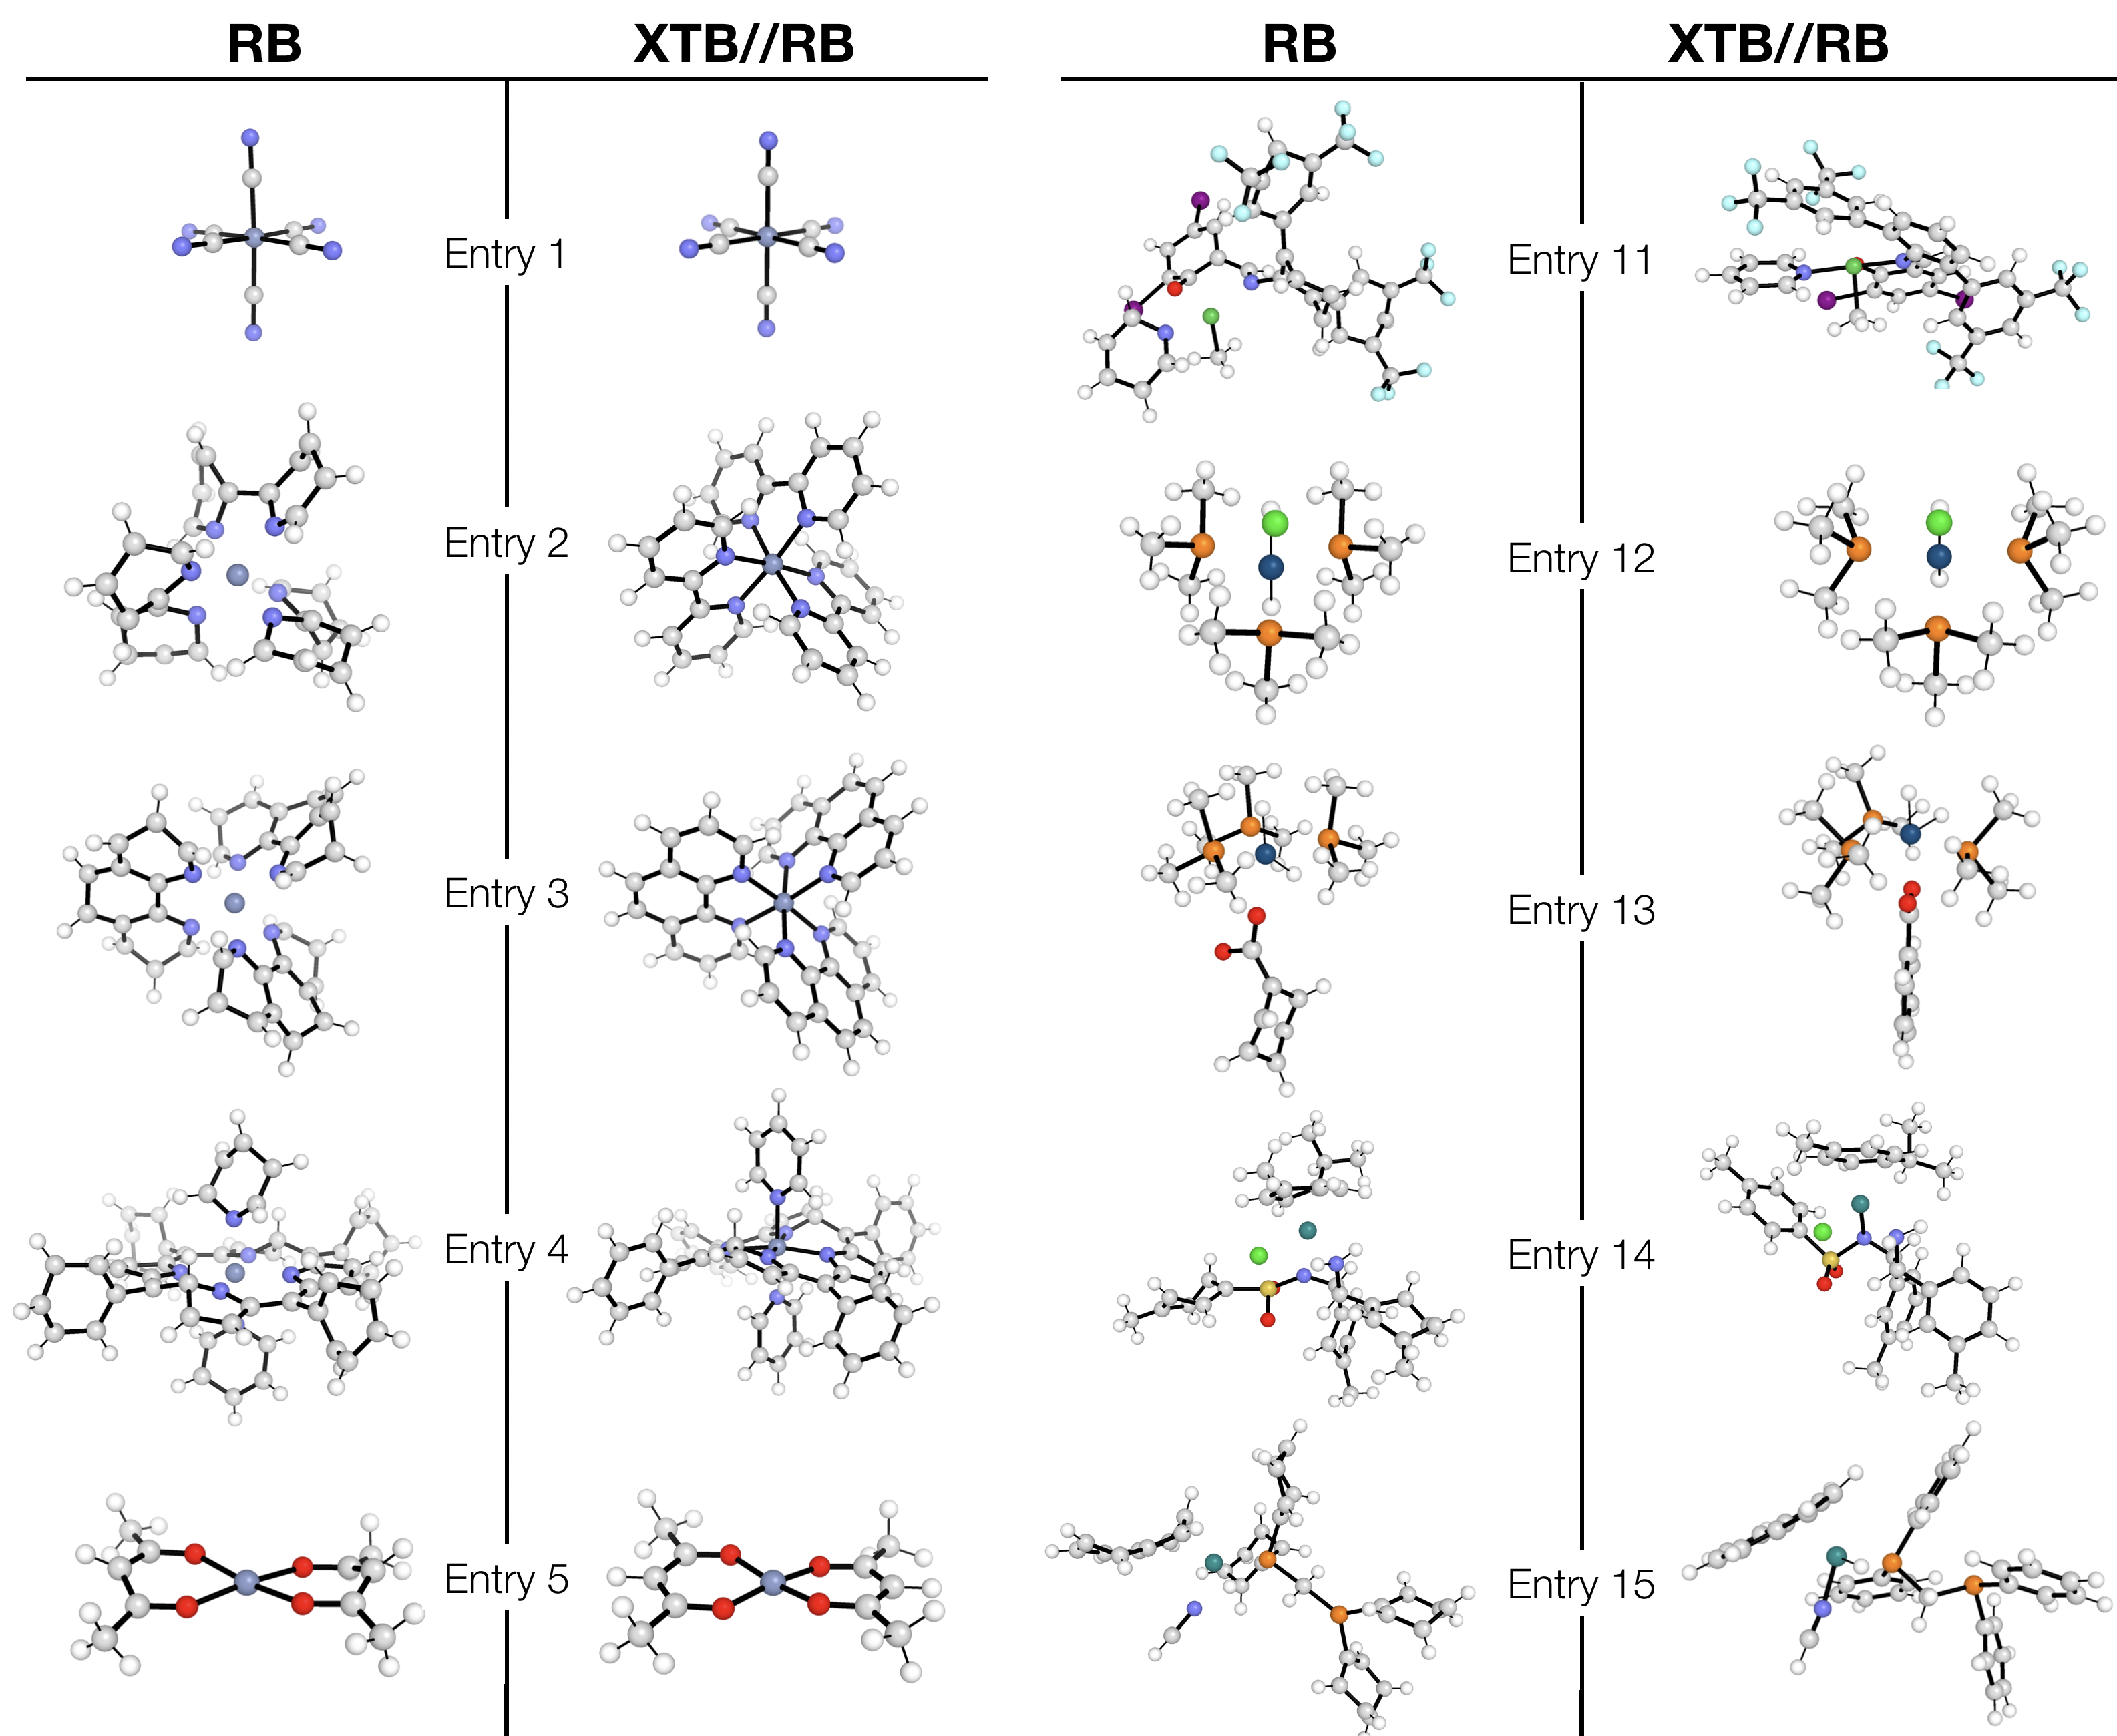
\includegraphics[width=\textwidth]{5/autode/figs/figS5a}
	\vspace{0.4cm}
	\hrule
	\caption{Metal complexes itemized in Table \ref{table::ade_si_1} generated by minimizing a simple repulsion + bonded potential Eqn. \eqref{equation::ade_1_repeat} and their subsequent XTB optimised geometries. Structures initialized by adding atoms sequentially from a random position within a 10 \AA$\;$ cube and minimizing $U-\text{RB}$ with $n$ = 2 repeatedly until all atoms were added, then performing a final minimization with $n = 8$ $(k = 1$, $c = 0.01)$.}
	\label{fig::ade_si_5a}
\end{figure}


\begin{figure}[h!]
	\vspace{0.4cm}
	\centering
	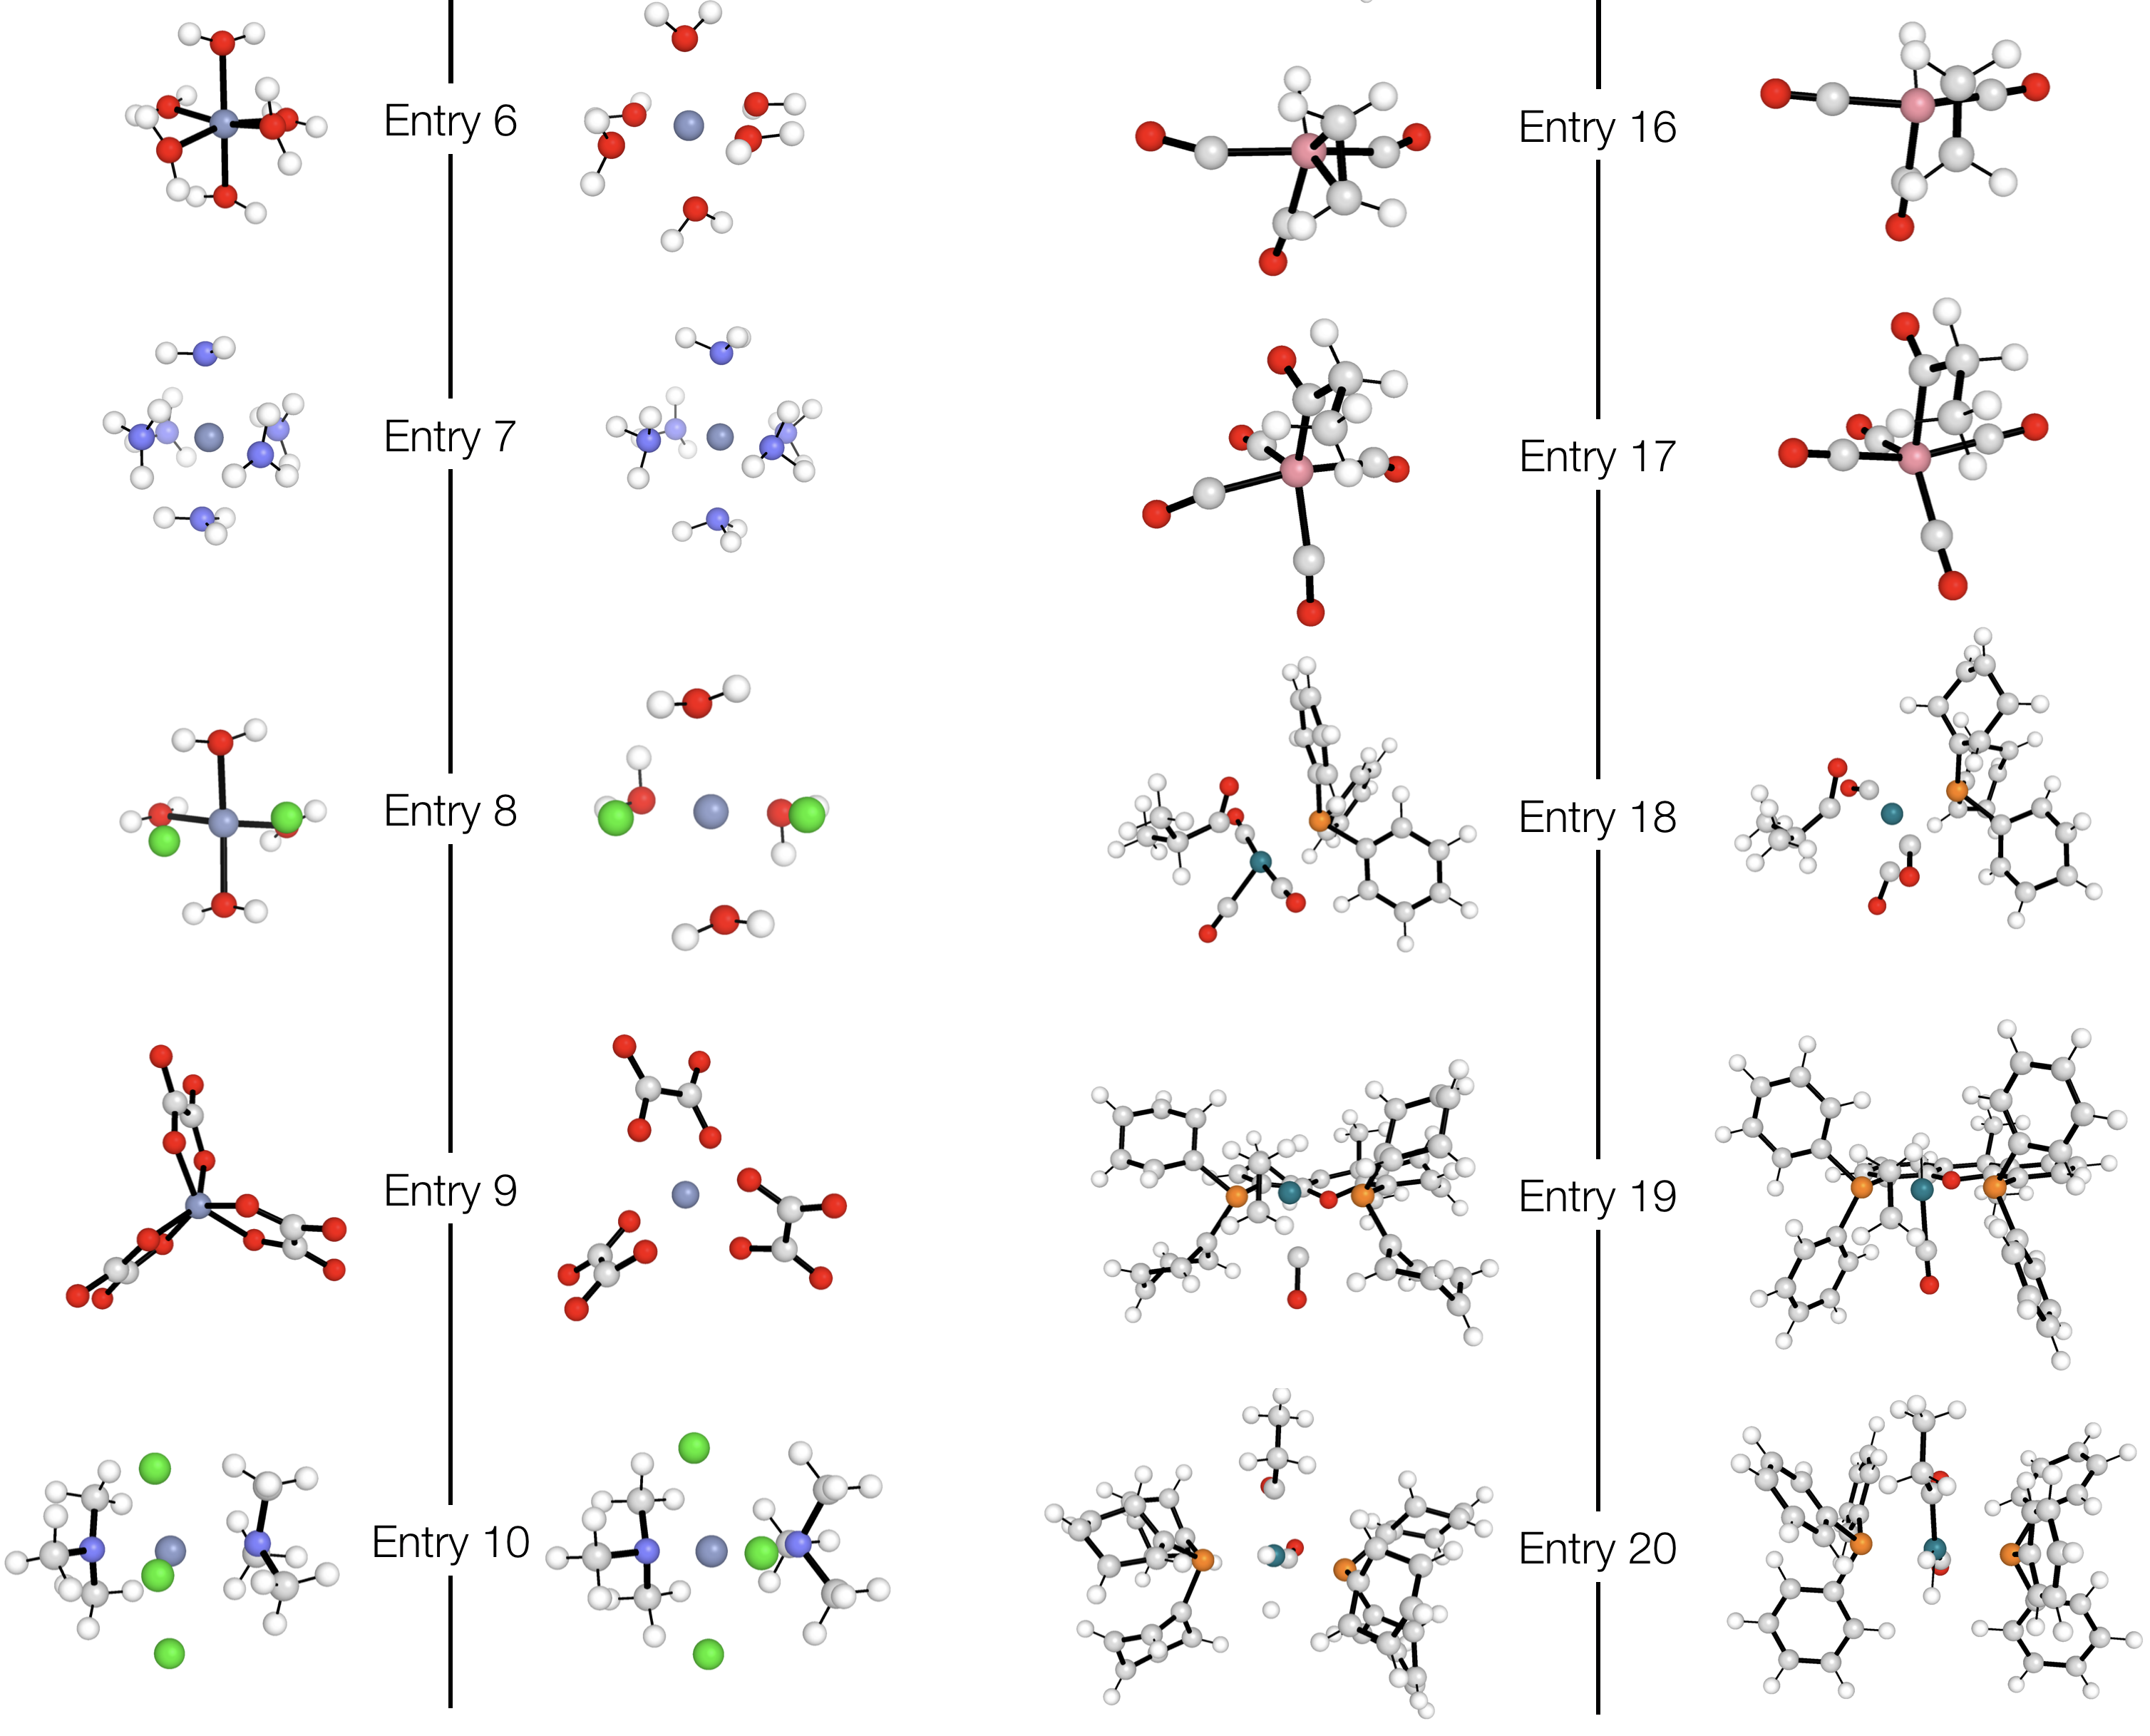
\includegraphics[width=\textwidth]{5/autode/figs/figS5b}
	\vspace{0.4cm}
	\hrule
	\caption{\figurename{ }\ref{fig::ade_si_5a} continued.}
	\label{fig::ade_si_5b}
\end{figure}



\begin{table}[h!]
	\def\arraystretch{1.5}
	\begin{tabularx}{\textwidth}{YYYYYYY}
		\hline
		Entry &	\multicolumn{2}{c}{RDKit}	& \multicolumn{2}{c}{CONFAB}	&\multicolumn{2}{c}{RB}
\\
		& 	SG &	N&	SG	&N	&SG	&N
	\\
		\hline

		1	&	 	\ding{55}	&0&	\ding{55}	&0	&\ding{51}	&1\\
		2	&	 	\ding{51}&	1&	\ding{55}	&0	&\ding{51}	&2
\\
		3	& 	\ding{51}	&1	&\ding{55}	&0	&\ding{51}	&5
\\
		4	&	\ding{51}	&15	&\ding{55}&	0&	\ding{51}&	17
\\
		5	& 	\ding{51}&	1&	\ding{55}	&0	&\ding{51}	&8
\\
		6	& 	\ding{55}&	0&	\ding{55}	&0&	\ding{51}	&10
\\
		7	& 	\ding{55}	&0	&\ding{55}	&0&	\ding{51}&	1
\\
		8 & 	\ding{55}&	0&	\ding{55}&	0&	\ding{51}&	10
\\
		9	&	\ding{51}	&2&\ding{55}&	0&	\ding{51}	&1
\\
		10	&	\ding{51}&	2&\ding{55}	&0	&\ding{51}	&5
\\
		11	& 	\ding{51}&	6&	\ding{55}&	0	&\ding{51}	&23
\\
		12	& 	\ding{51}&	8&	\ding{55}	&0	&\ding{51}	&16
\\
		13	&	\ding{51}&	9&	\ding{55}	&0	&\ding{51}	&18
\\
		14	&	\ding{55}&	0	&\ding{55}&	0	&\ding{51}&	20
\\
		15	& 	\ding{51}	&22	&\ding{55}	&0&	\ding{51}	&24
\\
		16	& 	\ding{51}	&1	&\ding{55}	&0	&\ding{51}	&5
\\
		17 &	\ding{51}&	3&	\ding{55}	&0&	\ding{51}&	5
\\
		18	&	\ding{51}&	13	&\ding{55}&	0&	\ding{51}	&18
\\
		19	&	\ding{51}&	14&	\ding{55}&	0&	\ding{51}&	19
\\
		20	&	\ding{51}&	28	&\ding{55}	&0&	\ding{51}	&30
		
	\end{tabularx}
	\label{table::si_ade_1}
	\hrule
	\caption{Metal complex test set. The set comprises the first 10 complexes used to benchmark MolSimplify (ref. \cite{Ioannidis2016}., all Cr(II)), 5 large complexes from ref. \cite{Ounkham2017} and 5 intermediates in hydroformylation catalysis. N is the number of conformers/isomers generated using RDKit (v. 2019.09.3), CONFAB (OpenBabel v. 2.4.1), and the repulsion + bonded (RB, Eqn. \eqref{equation::ade_3}) algorithm introduced in this work. Unique conformers are found by discarding those with energies within 0.24 \kcalx of others. RDKit and RB requested 50 conformers and CONFAB the default. 3D structure generated (SG) successfully is indicated with a  tick. See full supporting information for SMILES strings and \figurename{ \ref{fig::ade_si_5a}, \ref{fig::ade_si_5b}} for geometries.}
	\label{table::ade_si_1}
\end{table}




\begin{figure}[h!]
	\vspace{0.4cm}
	\centering
	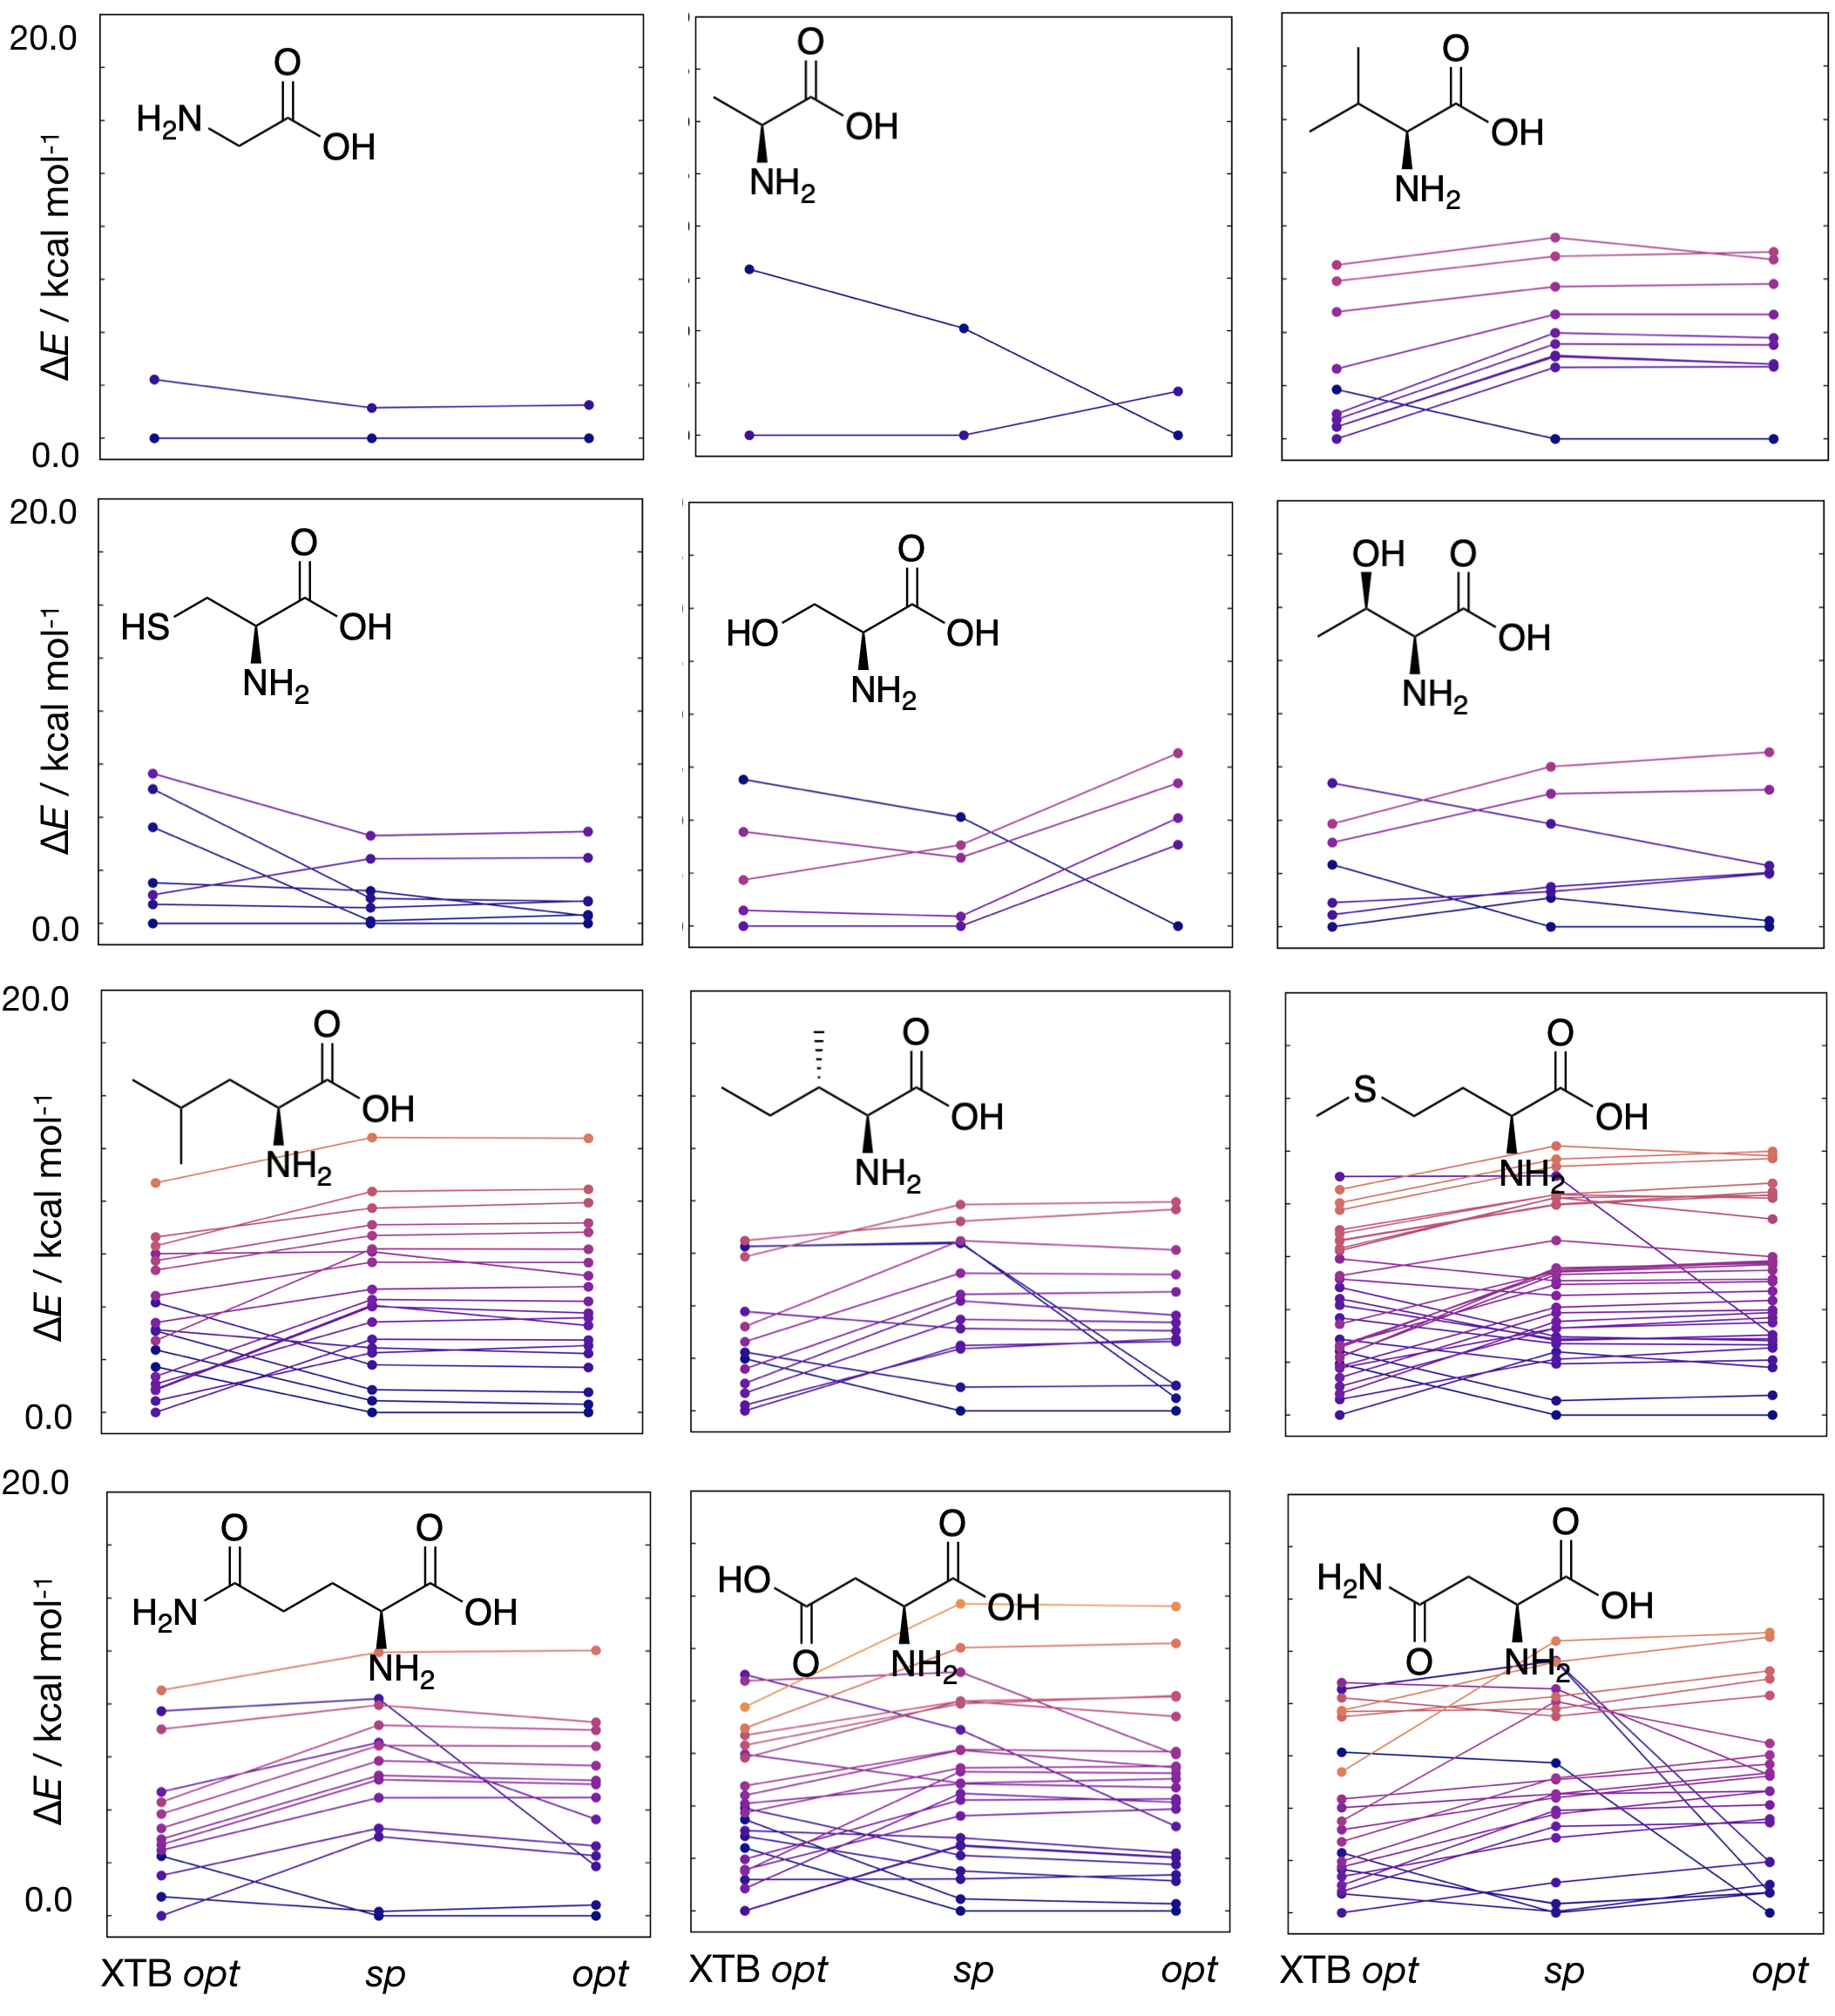
\includegraphics[width=\textwidth]{5/autode/figs/figS6a}
	\vspace{0.4cm}
	\hrule
	\caption{Conformer ranking for 20 amino acids in their neutral form using energies from XTB optimization (XTB opt), DFT single points (sp, XTB optimised geometries) and DFT loose optimization (opt). DFT calculations performed at the PBE-D3BJ/def2-SVP level of theory. Conformers generated using RDKit with a maximum of 1000 requested and an RMSD threshold of 0.05 \AA.}
	\label{fig::ade_si_6a}
\end{figure}


\begin{figure}[h!]
	\vspace{0.4cm}
	\centering
	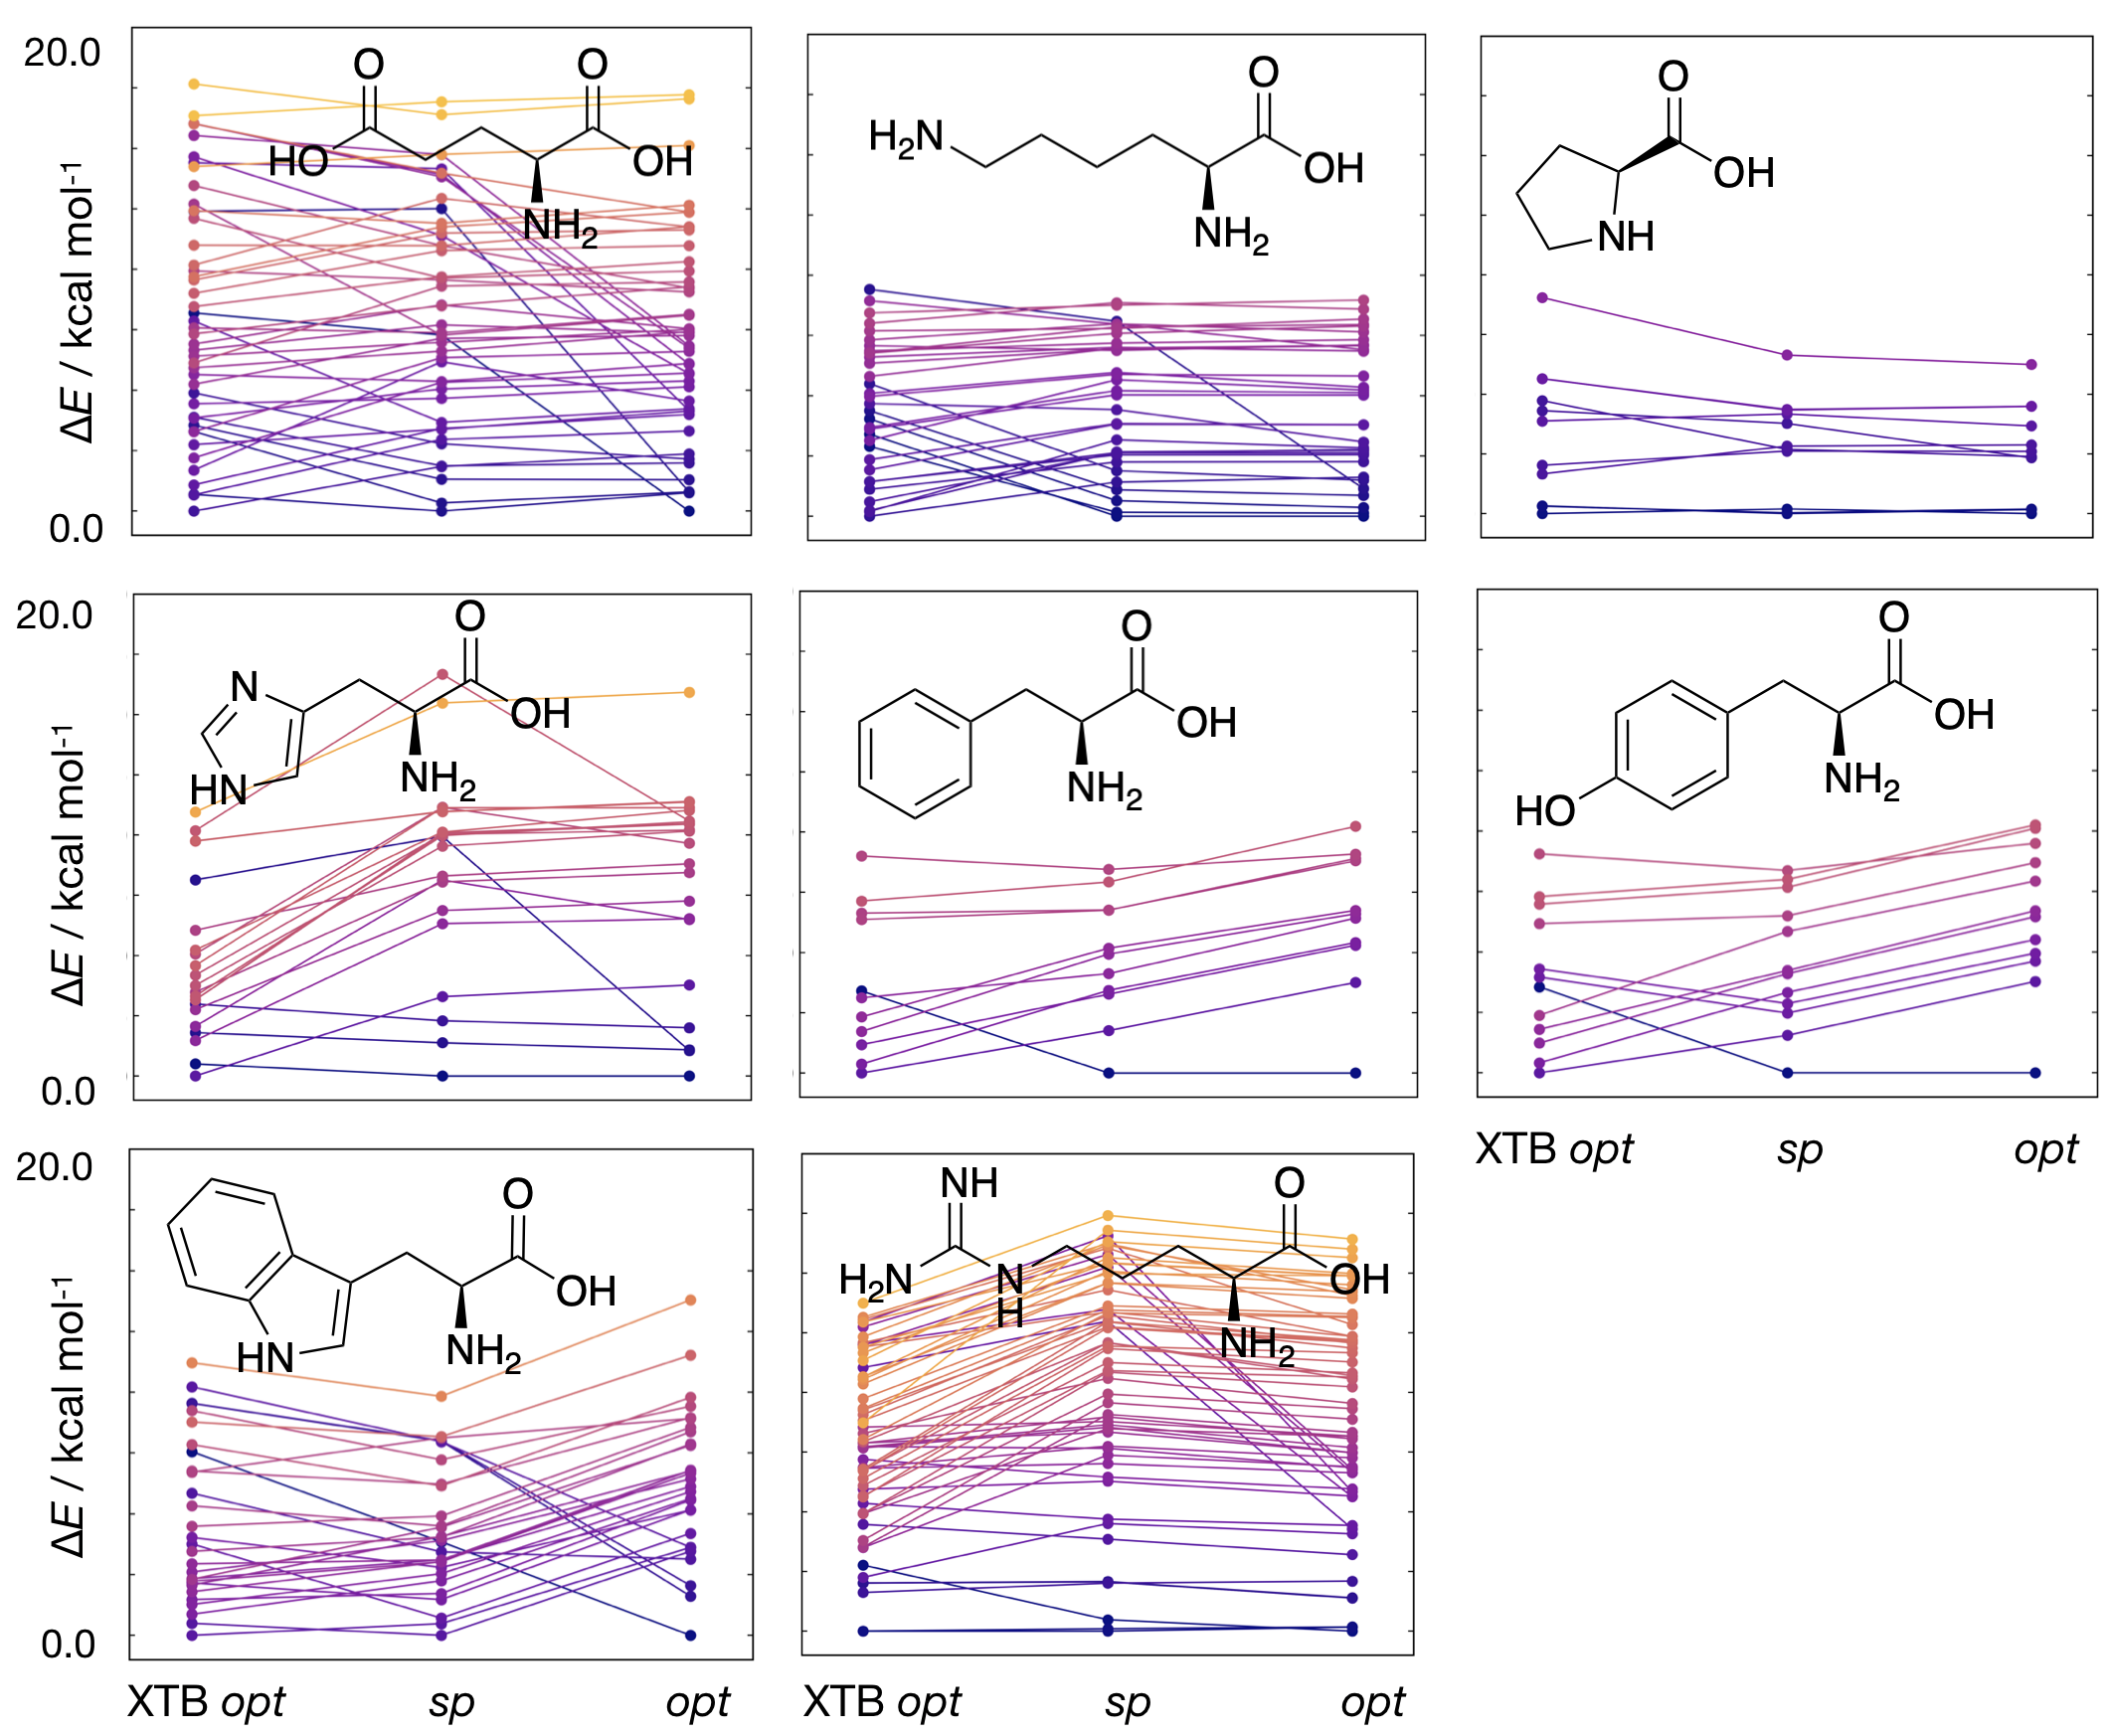
\includegraphics[width=\textwidth]{5/autode/figs/figS6b}
	\vspace{0.4cm}
	\hrule
	\caption{\figurename{ }\ref{fig::ade_si_6a} continued.}
	\label{fig::ade_si_6b}
\end{figure}

\clearpage
\subsection{Constructing Molecular Graphs}

The precise nature and properties of a chemical bond are still not uniquely defined,\cite{Zhao2019} this is despite a rather inclusive IUPAC definition of ‘When forces acting between two atoms or groups of atoms lead to the formation of a stable independent molecular entity, a chemical bond is considered to exist…’.\cite{IUPACgoldbook} However, to form a molecular graph the bonds must be rigidly defined. Given a SMILES string the molecular graph is constructed by adding edges defined explicitly (e.g. C=C) and implicitly (C--H) in the string. If a molecular graph is constructed from a 3D geometry an edge between two atoms (a, b) is added if $r_{ab} < 1.25 \times r^\text{avg}_{ab}$, where $r^\text{avg}_{ab}$ is the CCDC average for that atom pair (i.e. $r^\text{avg}_\text{C--C}$ = 1.427 \AA). Edges are added by iterating through atoms sorted by their atomic weight, then for each atom index $i$ enumerating atoms $j > i$ sorted by the distance closest to atom $i$. If an atom exceeds its maximal valance e.g. hydrogen: 1, carbon: 4 then the longest edge(s) is(are) removed. Some simple examples are shown in Figure \ref{fig::ade_si_7}. 



\begin{figure}[h!]
	\vspace{0.4cm}
	\centering
	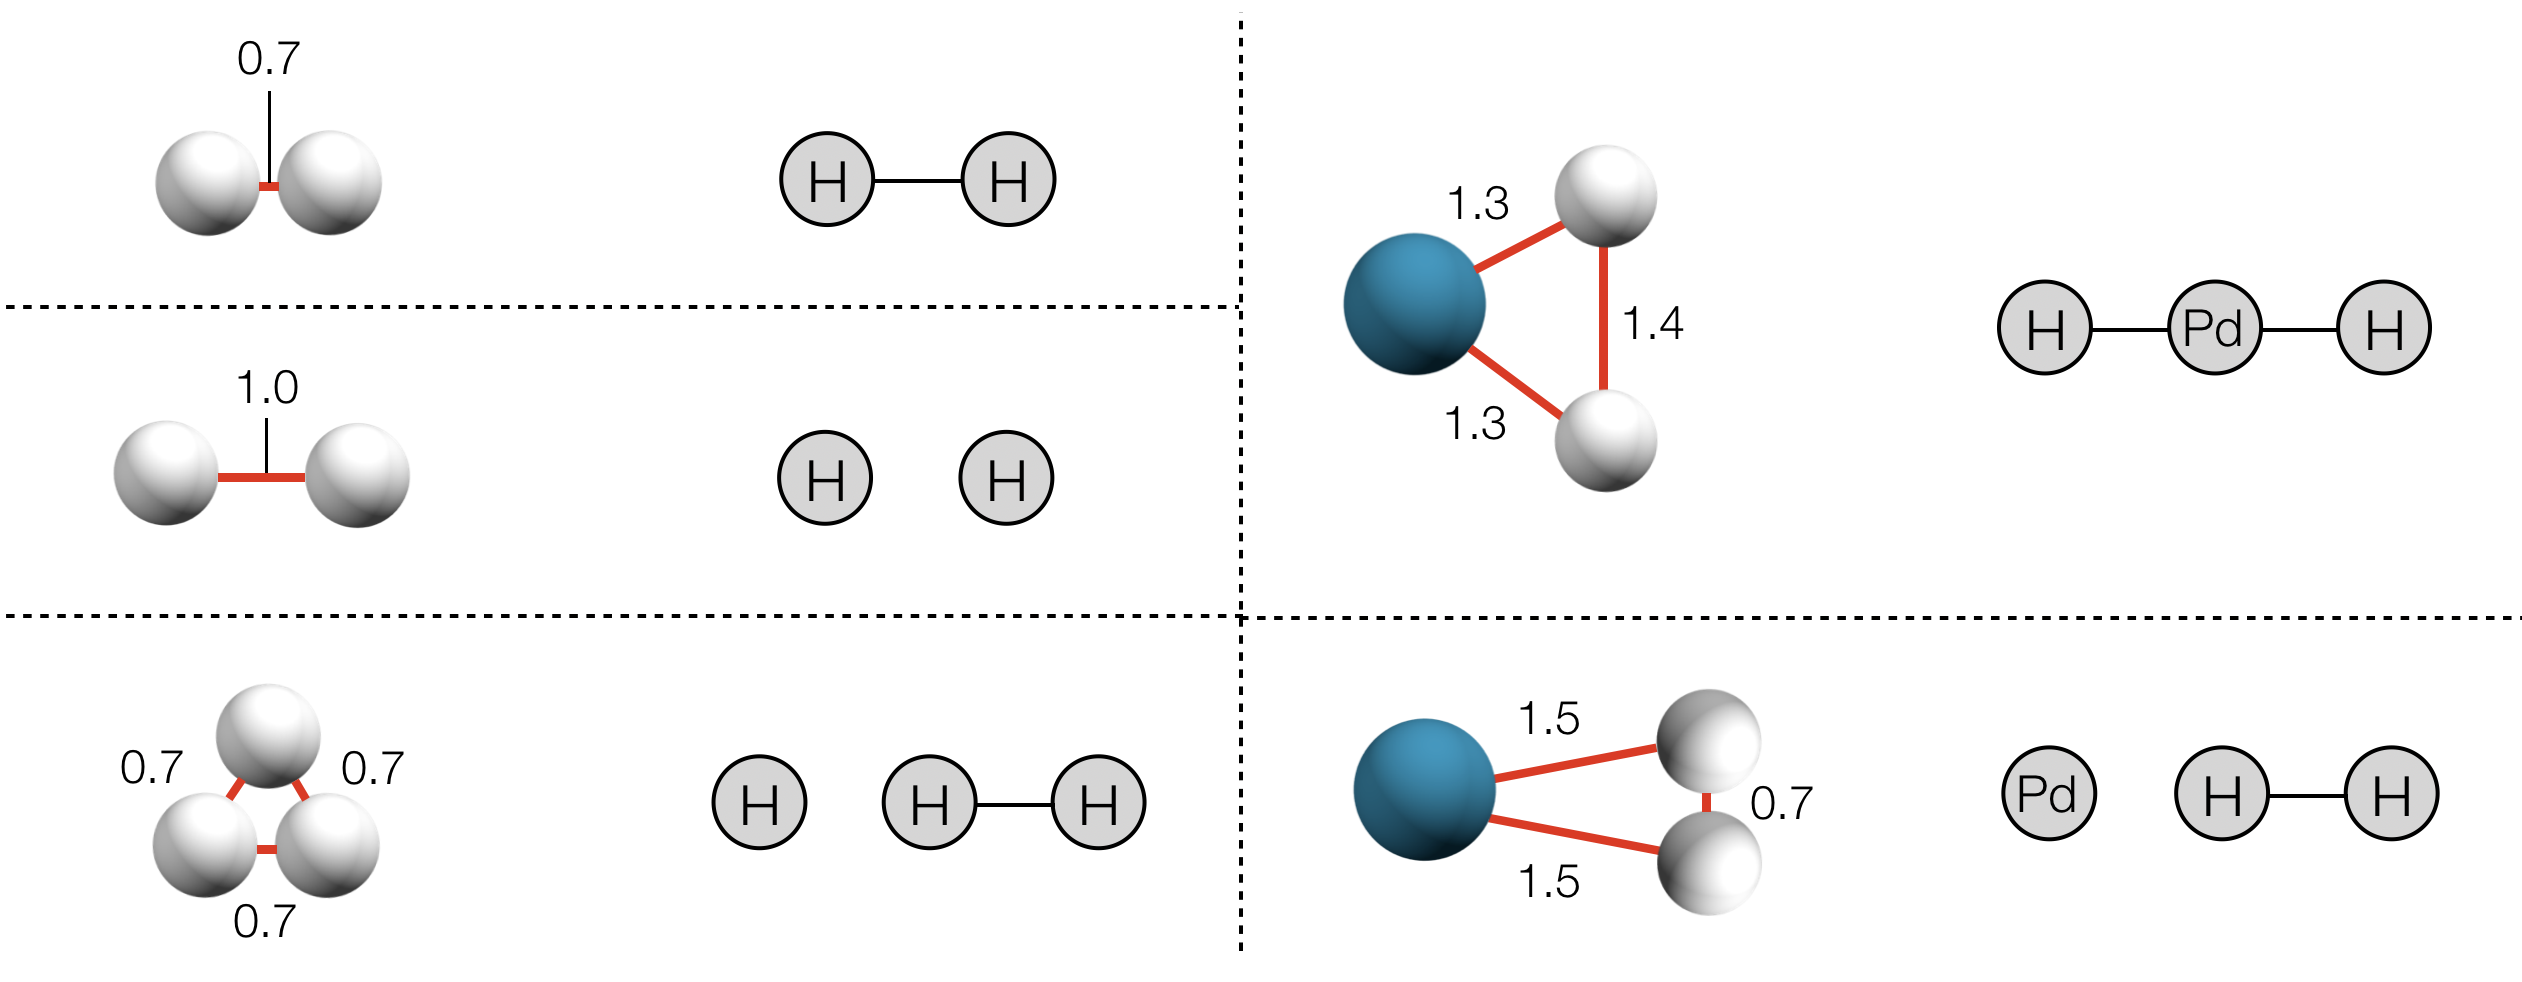
\includegraphics[width=14cm]{5/autode/figs/figS7}
	\vspace{0.4cm}
	\hrule
	\caption{Mapping of 3D structures to molecular graphs. Distances quoted in \AA.}
	\label{fig::ade_si_7}
\end{figure}


In the molecular graphs used here there is no concept of multiple bonding with the exception of allowing nodes to be ‘pi atoms’, so that suitable distance constraints can be added to ensure no rotation about $\pi$-bonds in RB conformer generation and a molecule is not truncated over a $\pi$-bond. A node may also be a ‘stereo atom’ which again is to prevent inversion of chiral centres in RB conformer generation.



\begin{figure}[h!]
	\vspace{0.4cm}
	\centering
	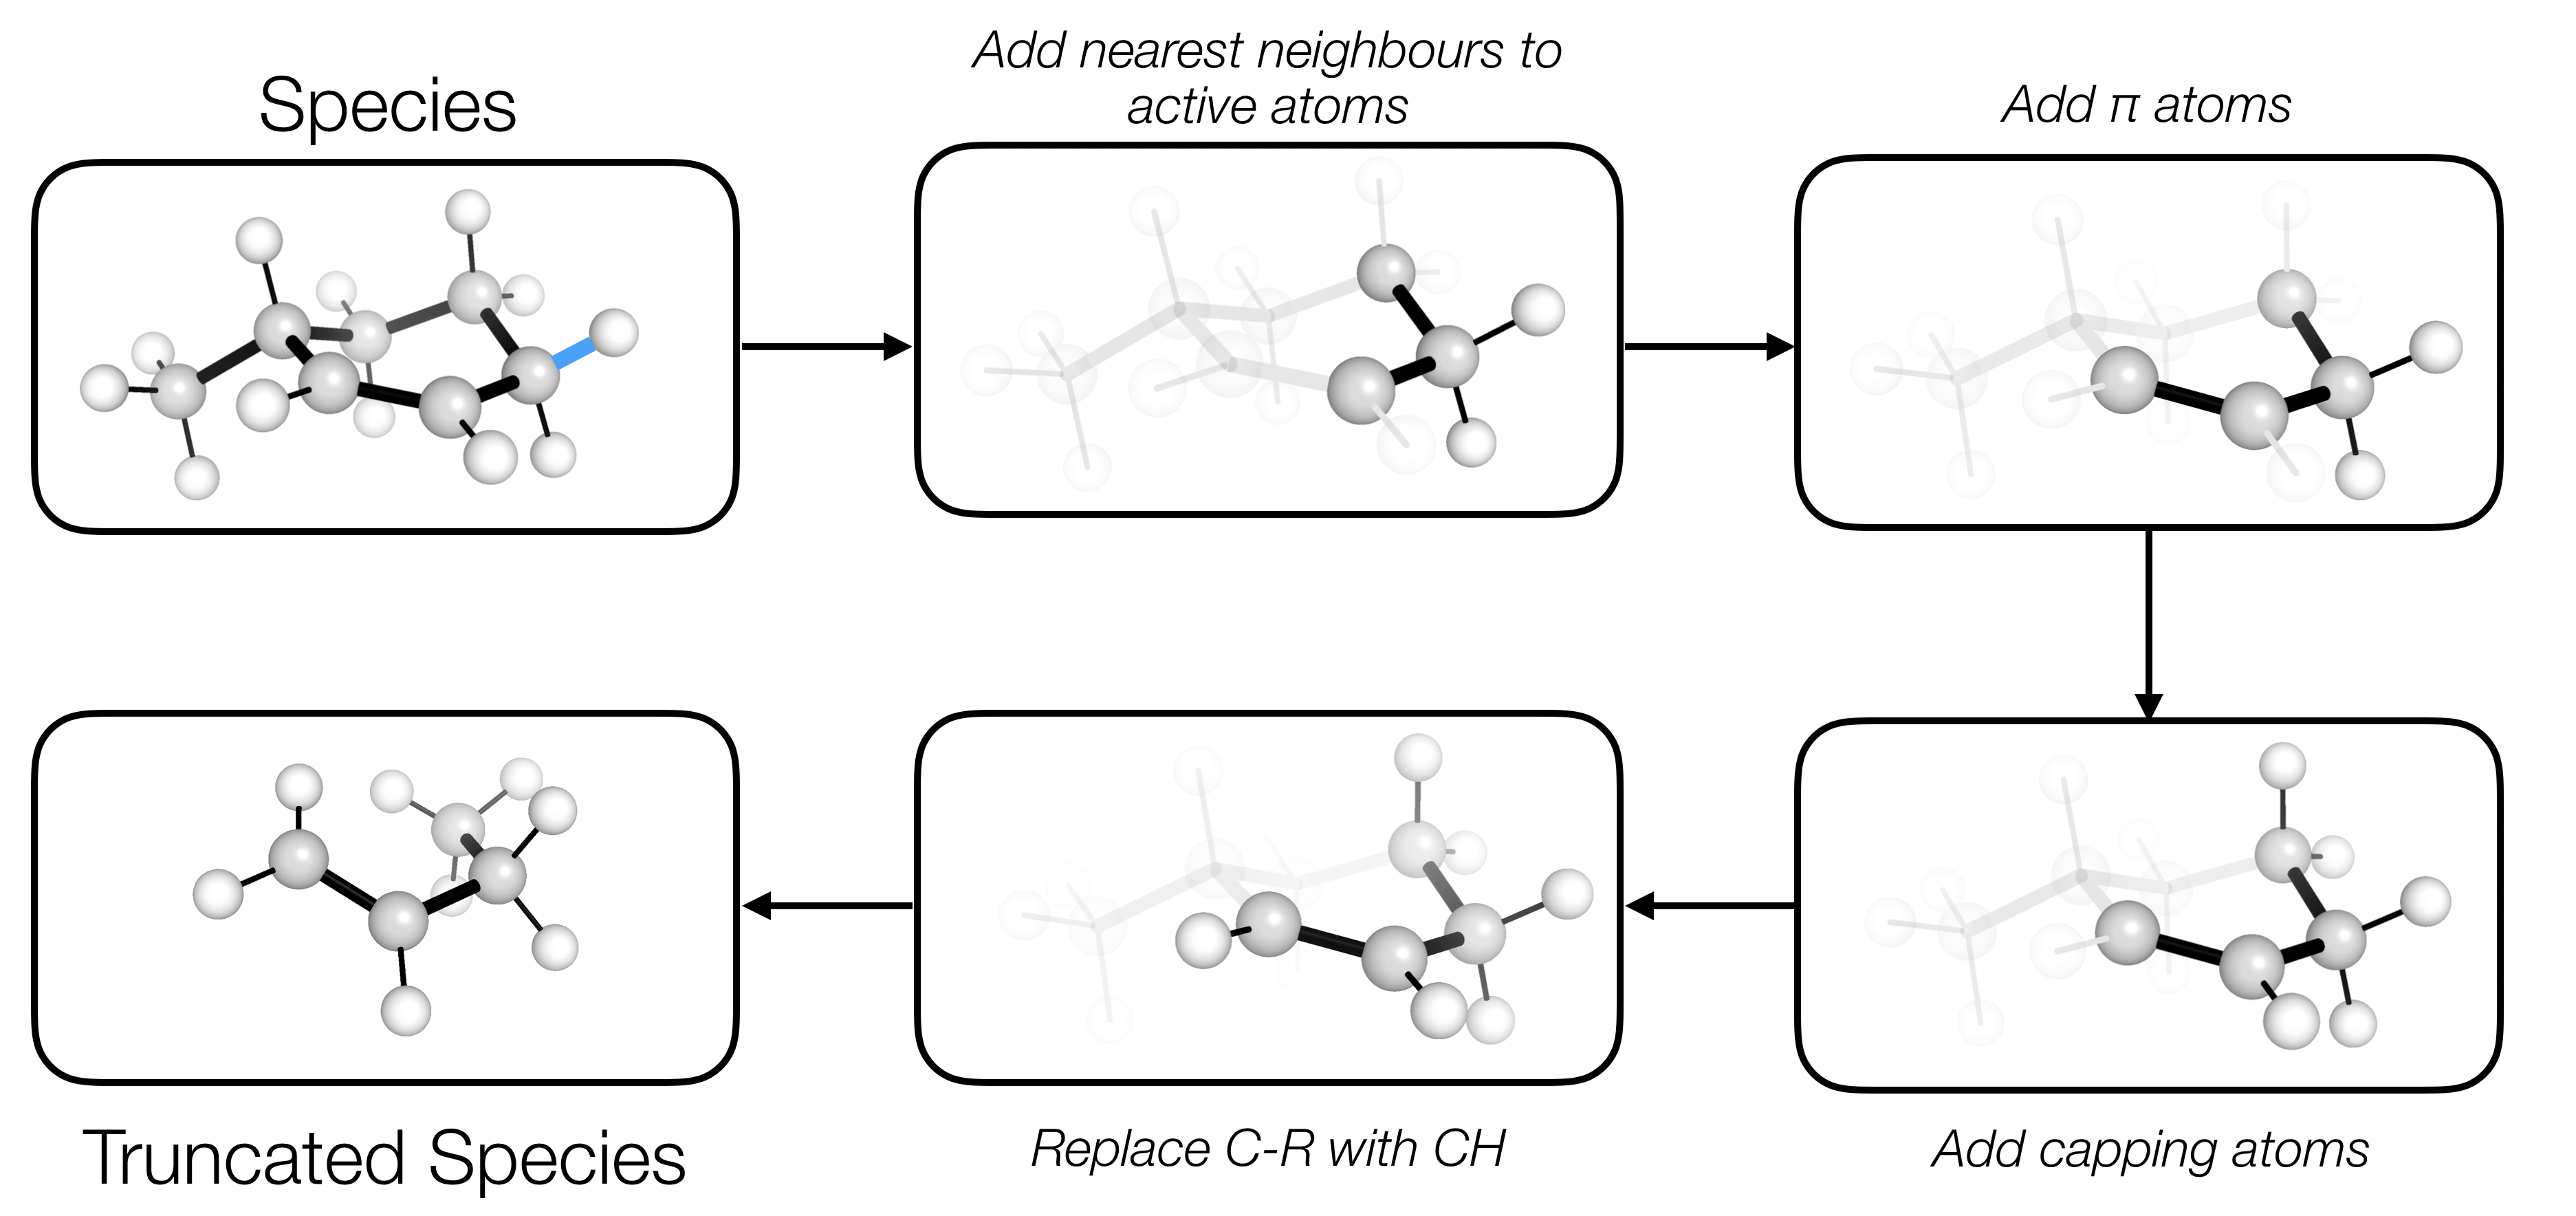
\includegraphics[width=14cm]{5/autode/figs/figS8}
	\vspace{0.4cm}
	\hrule
	\caption{Schematic process of truncating 3-methylcyclohex-1-ene. The active bond is highlighted in blue and the active atoms are those that form the active bond (C, H).}
	\label{fig::ade_si_8}
\end{figure}


\clearpage
\subsection{Non-covalent and Reactive Reactant Complexes}
\label{section::ade_si_nci_complexes}

In many chemical processes, the formation of a reactant/product complex precedes/follows the chemical step of interest, and is therefore fundamental to determine the kinetics of the process. In some cases, the molecular graph of the reactant and product complexes may not be isomorphic to the separated reactants and products. For example, in the base-catalysed hydrolysis of methyl acetate, loss of MeO$^{-}$ from the tetrahedral intermediate proceeds with concurrent deprotonation of the acid (Figure \ref{fig::ade_si_10}). Thus, to successfully characterize the TS as ‘good’, reactant and product complex conformers are required from which isomorphisms can be checked to the forward/reverse displaced species from the TS. This approach allows the lowest energy conformer of a non-covalent interaction (NCI) complex to be located systematically. For a complex formed by molecule A and B, conformers of the A.B complex are constructed by adding molecule B at points equally spaced on the surface of a sphere in a random orientation around A, then energy minimizing with an \lmethodx (Figure \ref{fig::ade_si_11}). For a complex with $N_m$ molecules using $N_s$ points on a sphere and $N_r$ random rotations, this approach generates $(N_s\times N_r)^{N_m–1}$ conformers. To maintain efficiency, a maximum threshold number of conformers is set (1000 by default). This approach also provides additional functionality, facilitating the generation of hydrogen bond complexes of relevance in anion-recognition without prior knowledge (Figure \ref{fig::ade_si_12}).



\begin{figure}[h!]
	\vspace{0.4cm}
	\centering
	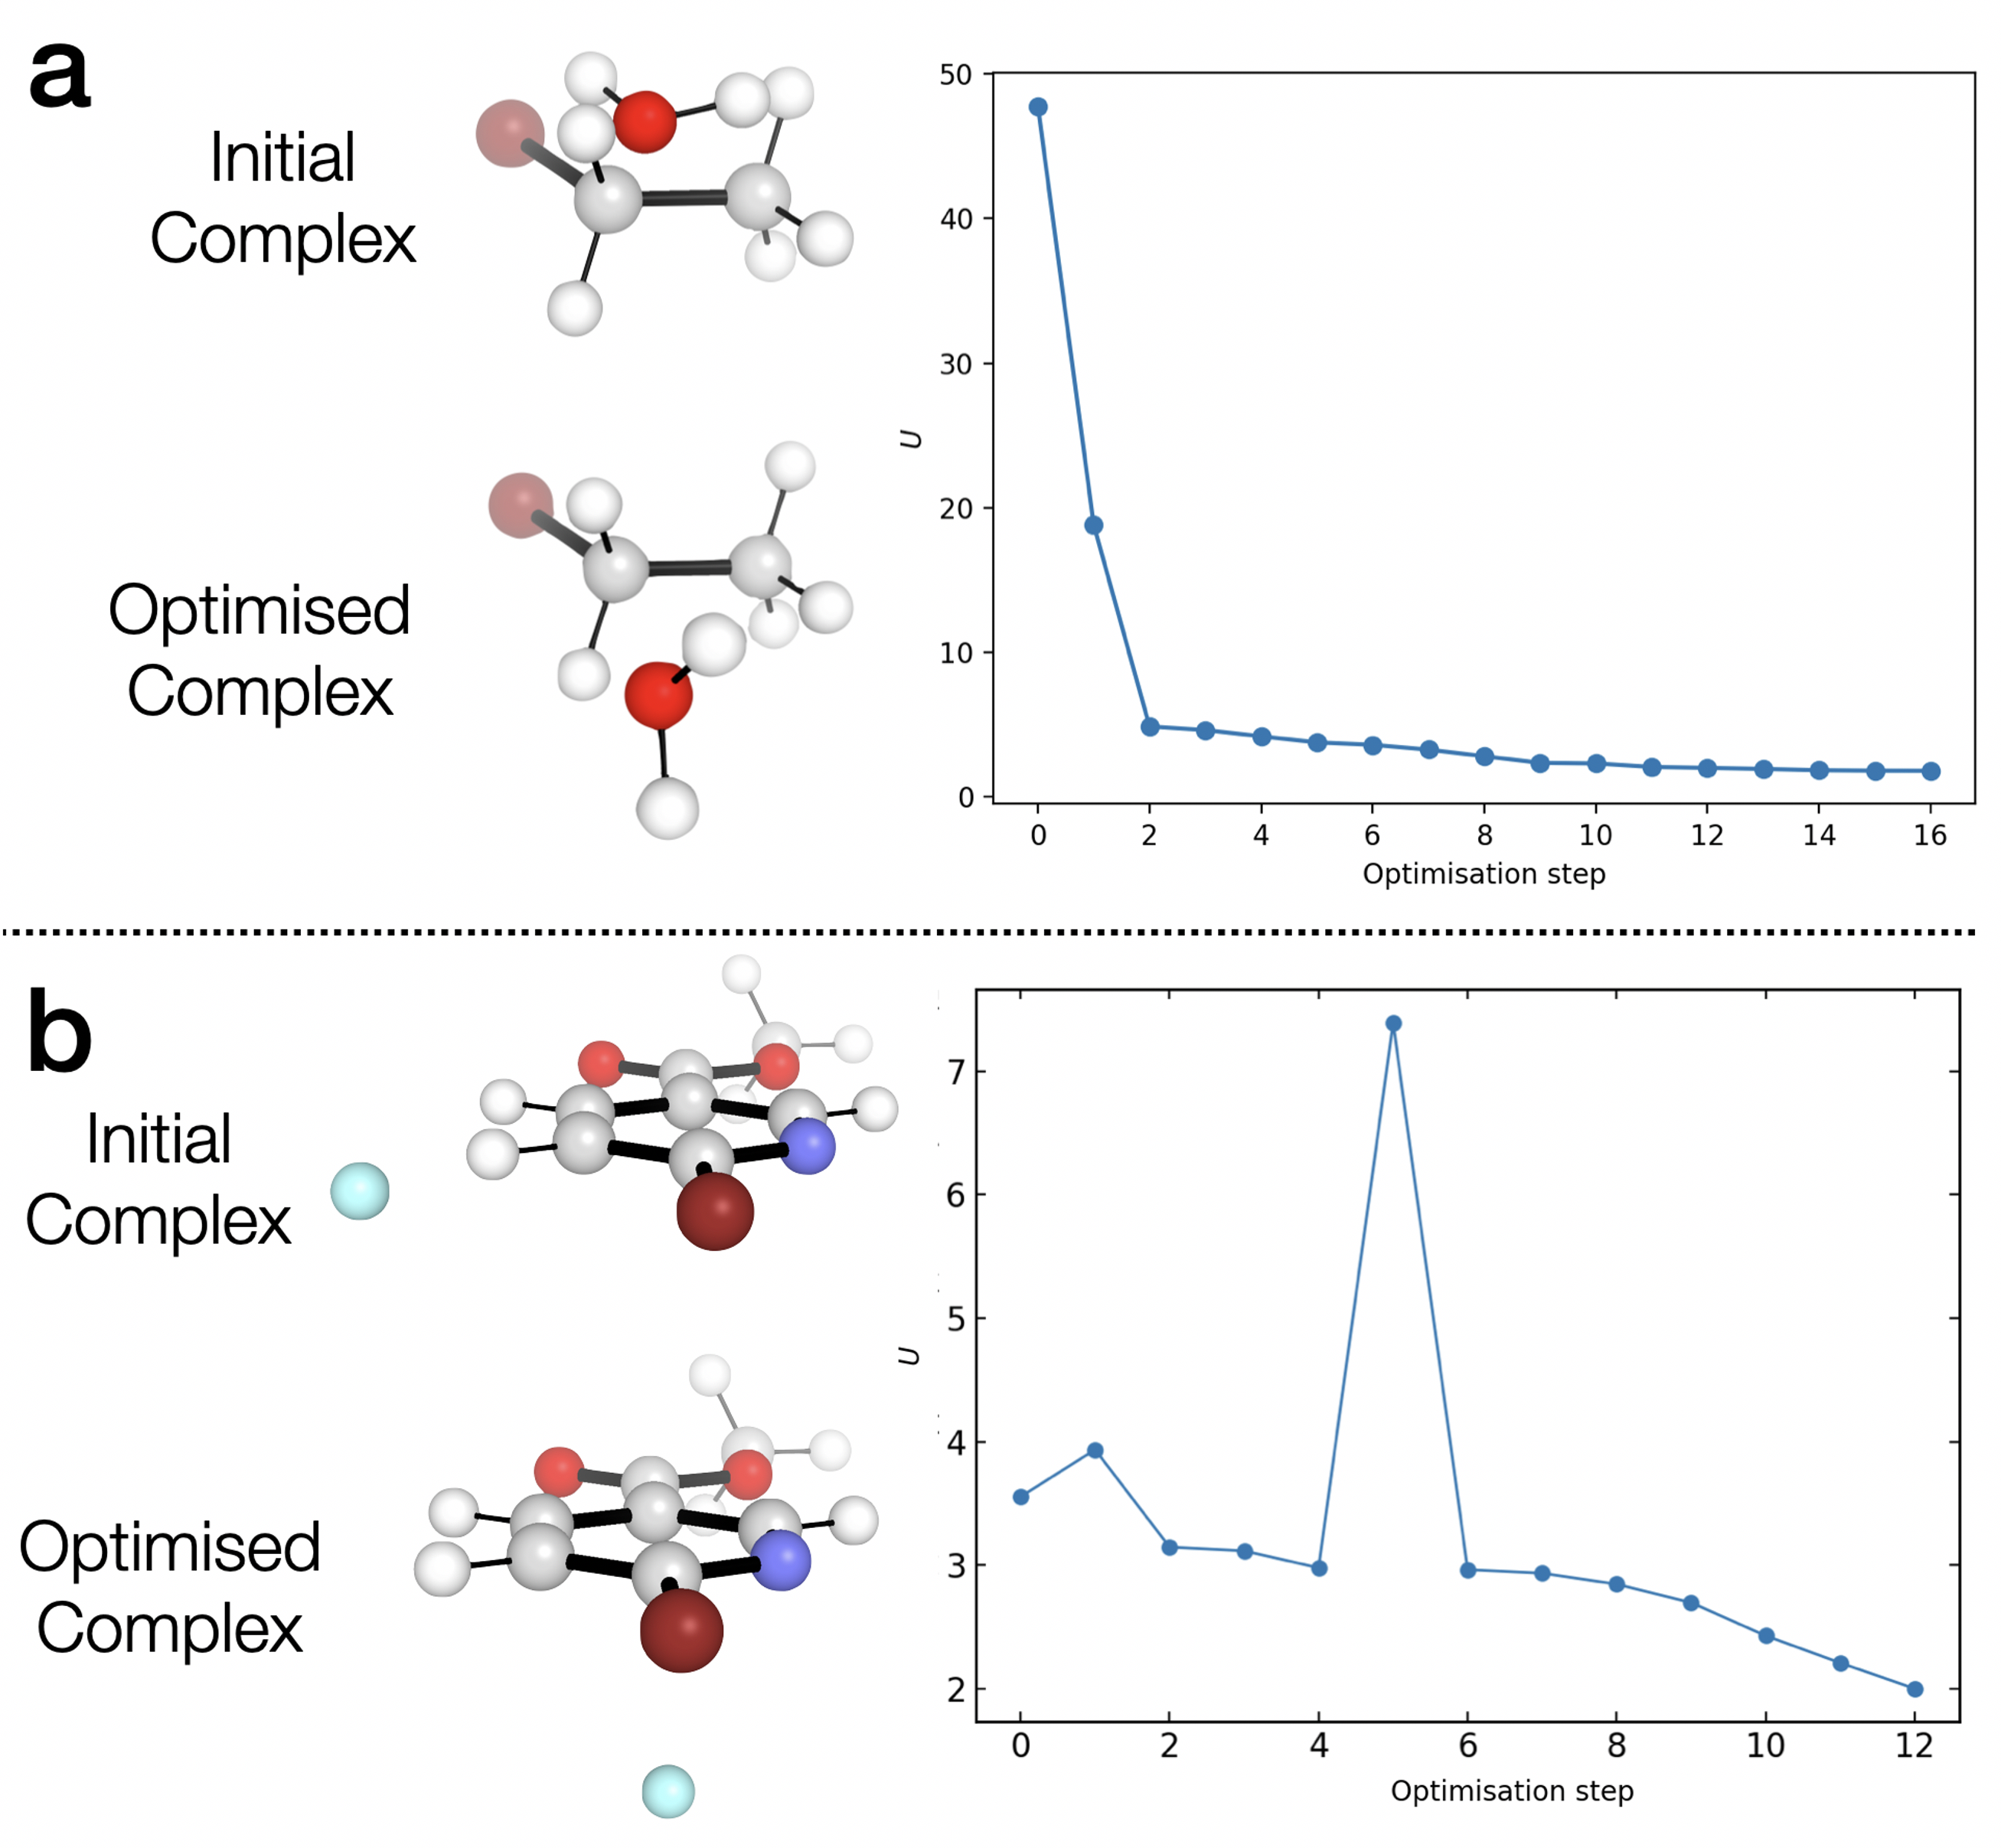
\includegraphics[width=12cm]{5/autode/figs/figS9}
	\vspace{0.4cm}
	\hrule
	\caption{Representative optimization of the reactant complexes for (a) ethylbromide + water and (b) methyl 6-bromonicotinate + fluoride (concerted S$_N$Ar from ref. \cite{Kwan2018}) under equation \eqref{equation::ade_3}. Energies ($U$) are in arbitrary units.}
	\label{fig::ade_si_9}
\end{figure}



\begin{figure}[h!]
	\vspace{0.4cm}
	\centering
	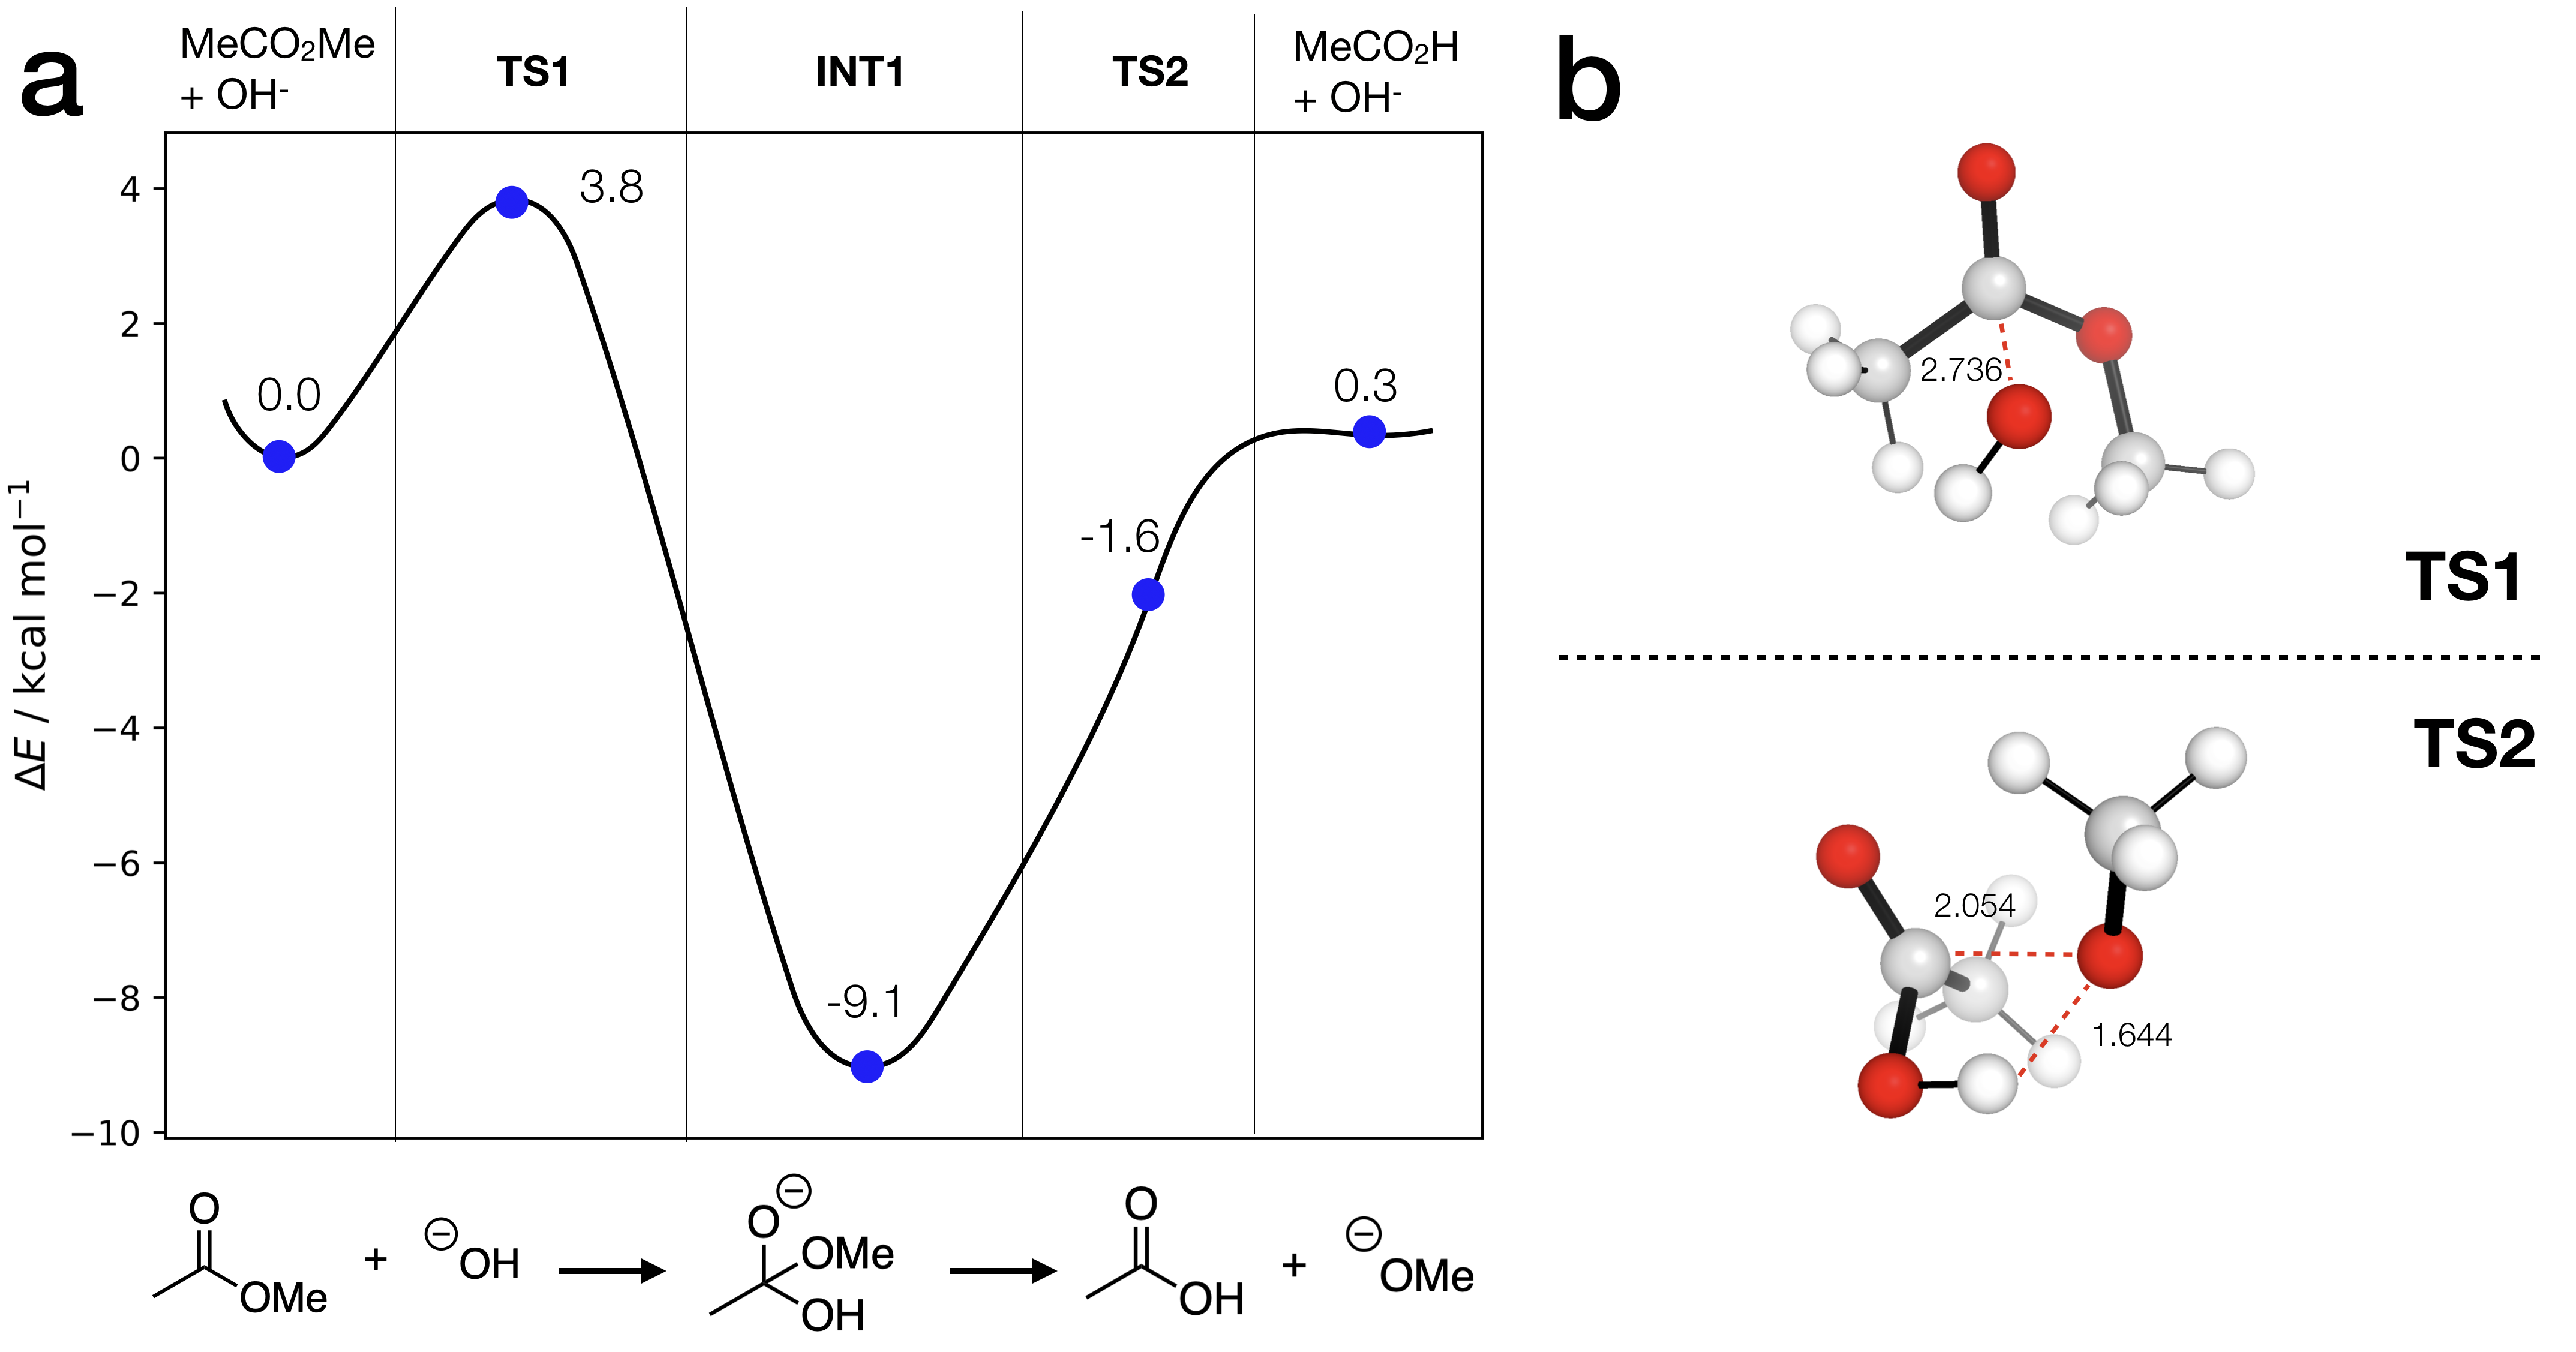
\includegraphics[width=\textwidth]{5/autode/figs/figS10}
	\vspace{0.4cm}
	\hrule
	\caption{(a) Reaction profile for alkaline ester hydrolysis generated in \ade (ORCA/XTB, CPCM(water)-PBE0-D3BJ/def2-TZVP//CPCM(water)-PBE0-D3BJ/ma-def2-SVP). TS for methoxide loss is more stable than separated acetic acid + methoxide species at the chosen level of theory. (b) TS structures calculated at CPCM(water)-PBE0-D3BJ/ma-def2-SVP. Key distances are quoted in \AA.}
	\label{fig::ade_si_10}
\end{figure}



\begin{figure}[h!]
	\vspace{0.4cm}
	\centering
	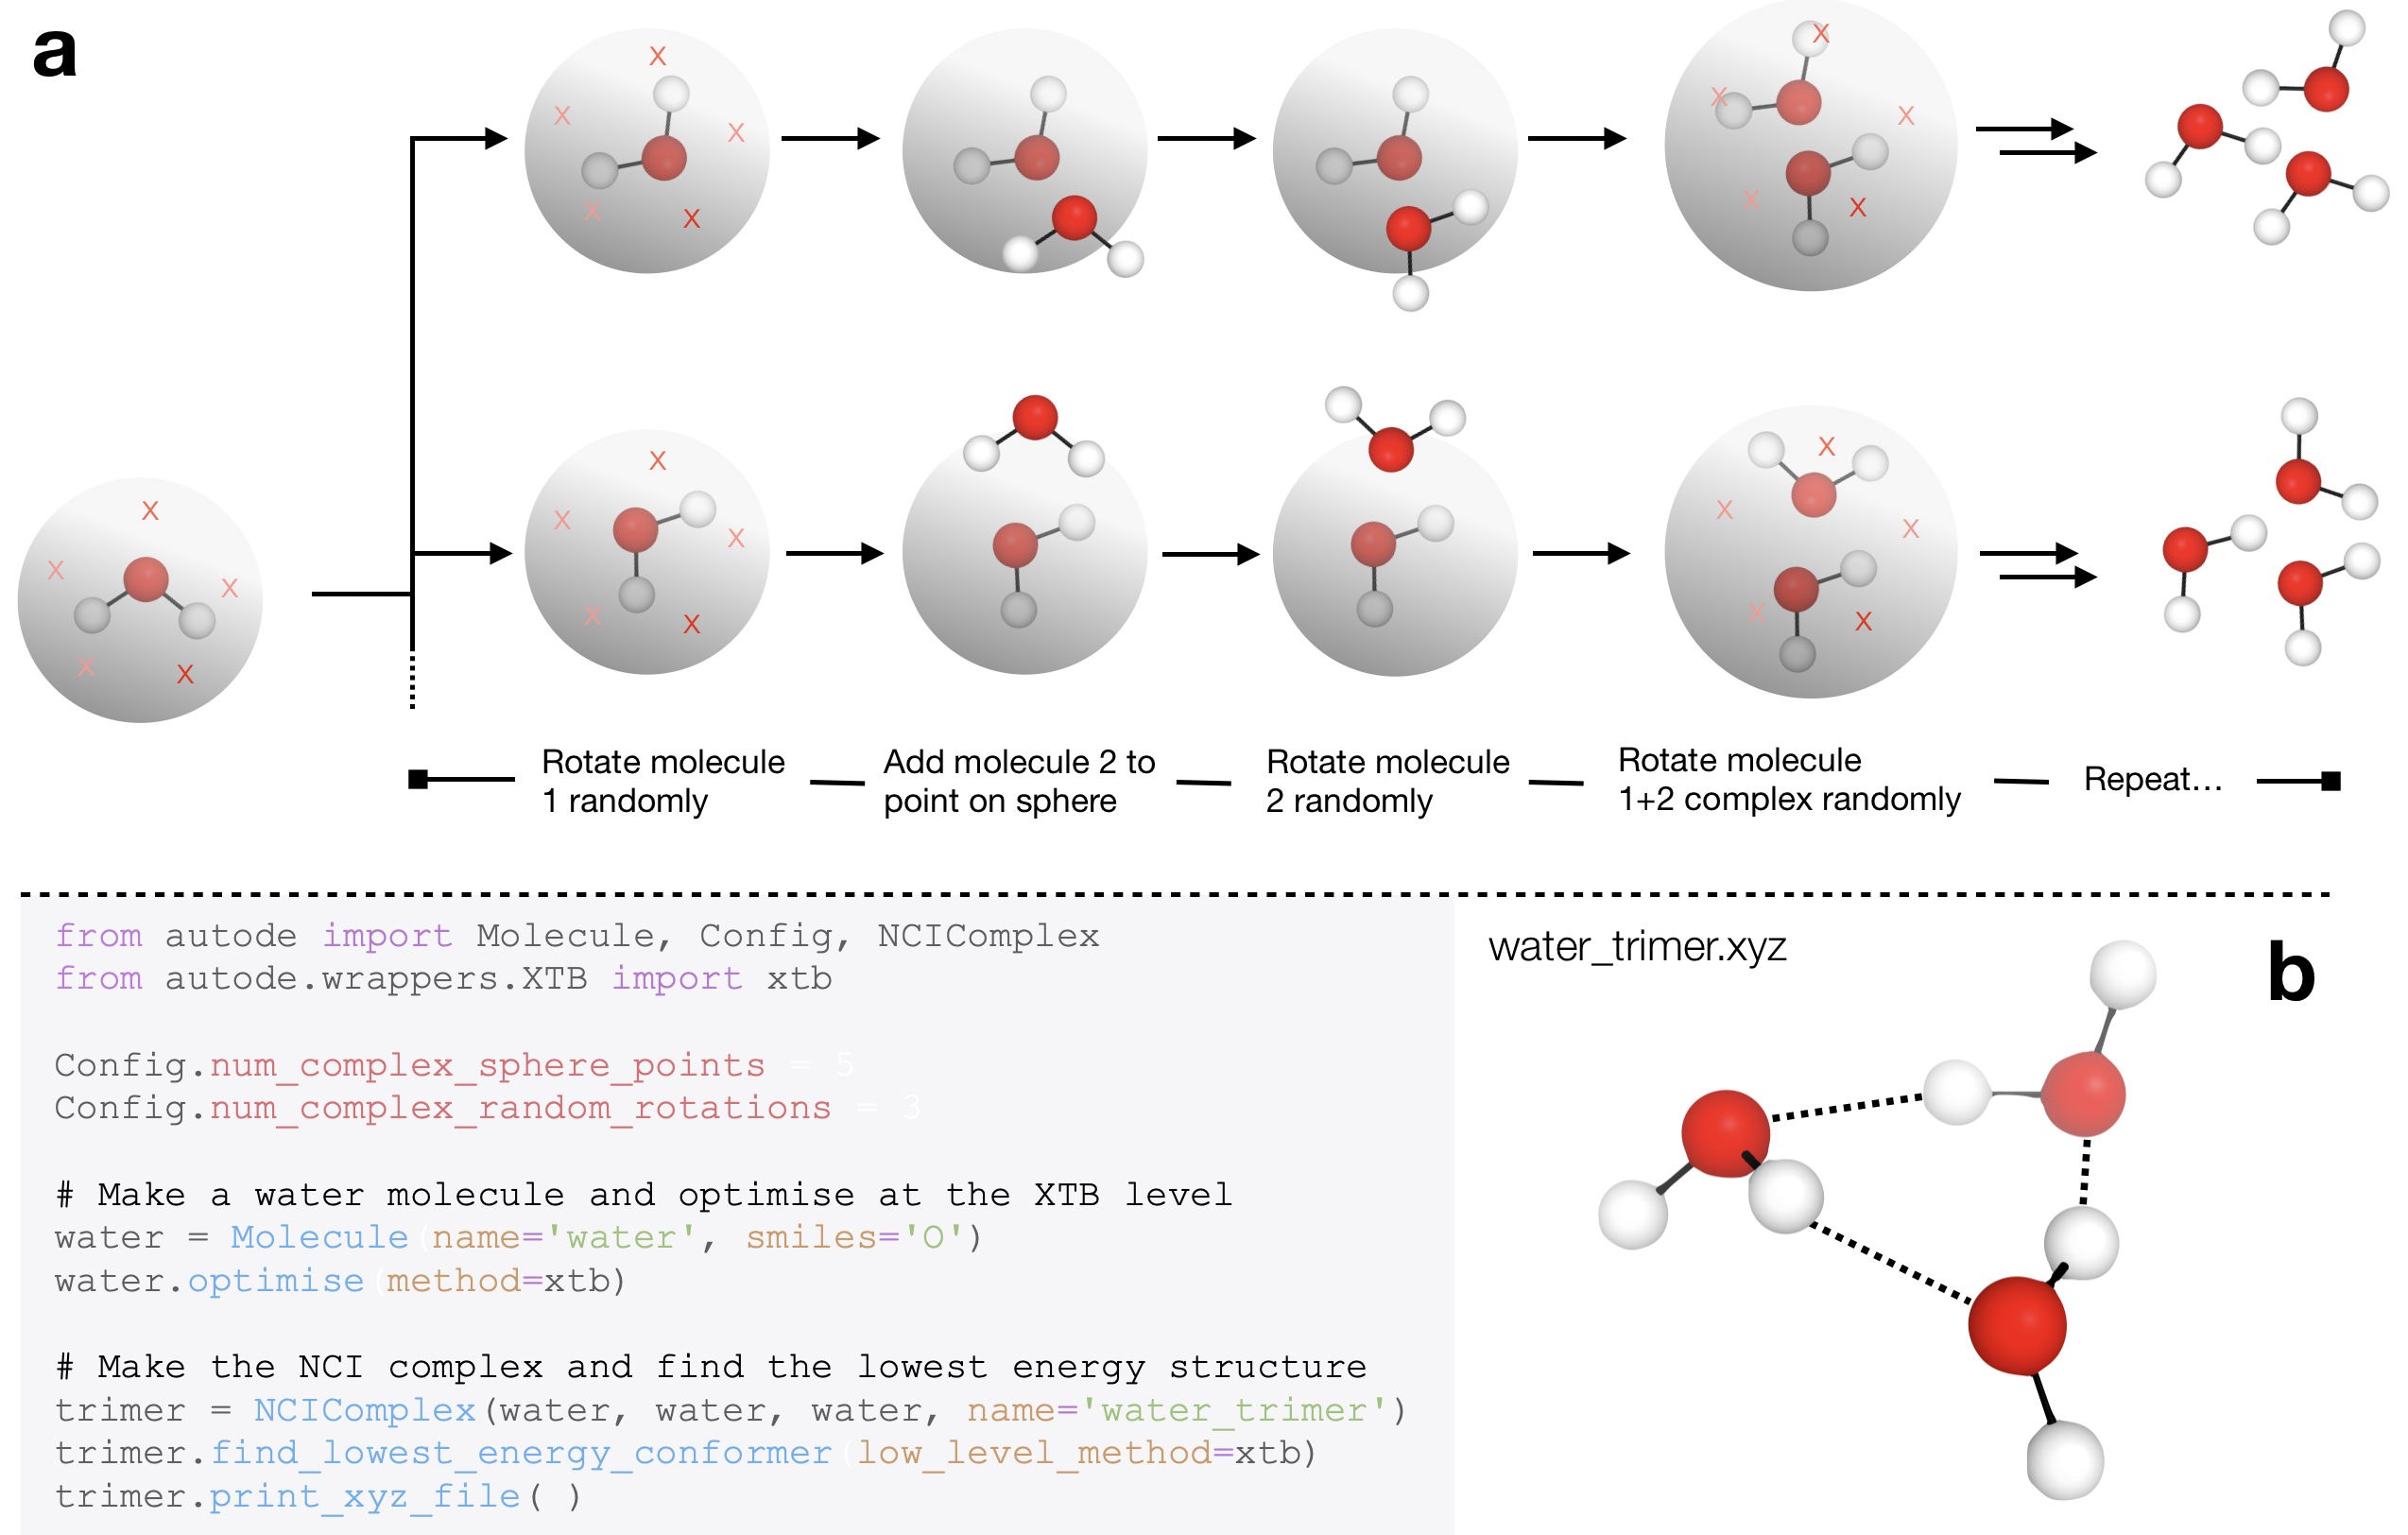
\includegraphics[width=\textwidth]{5/autode/figs/figS11}
	\vspace{0.4cm}
	\hrule
	\caption{NCI complex conformer (a) generation methodology and (b) application to the water trimer. $(5\times3)^2$ = 225 conformers are generated and optimised.}
	\label{fig::ade_si_11}
\end{figure}



\begin{figure}[h!]
	\vspace{0.4cm}
	\centering
	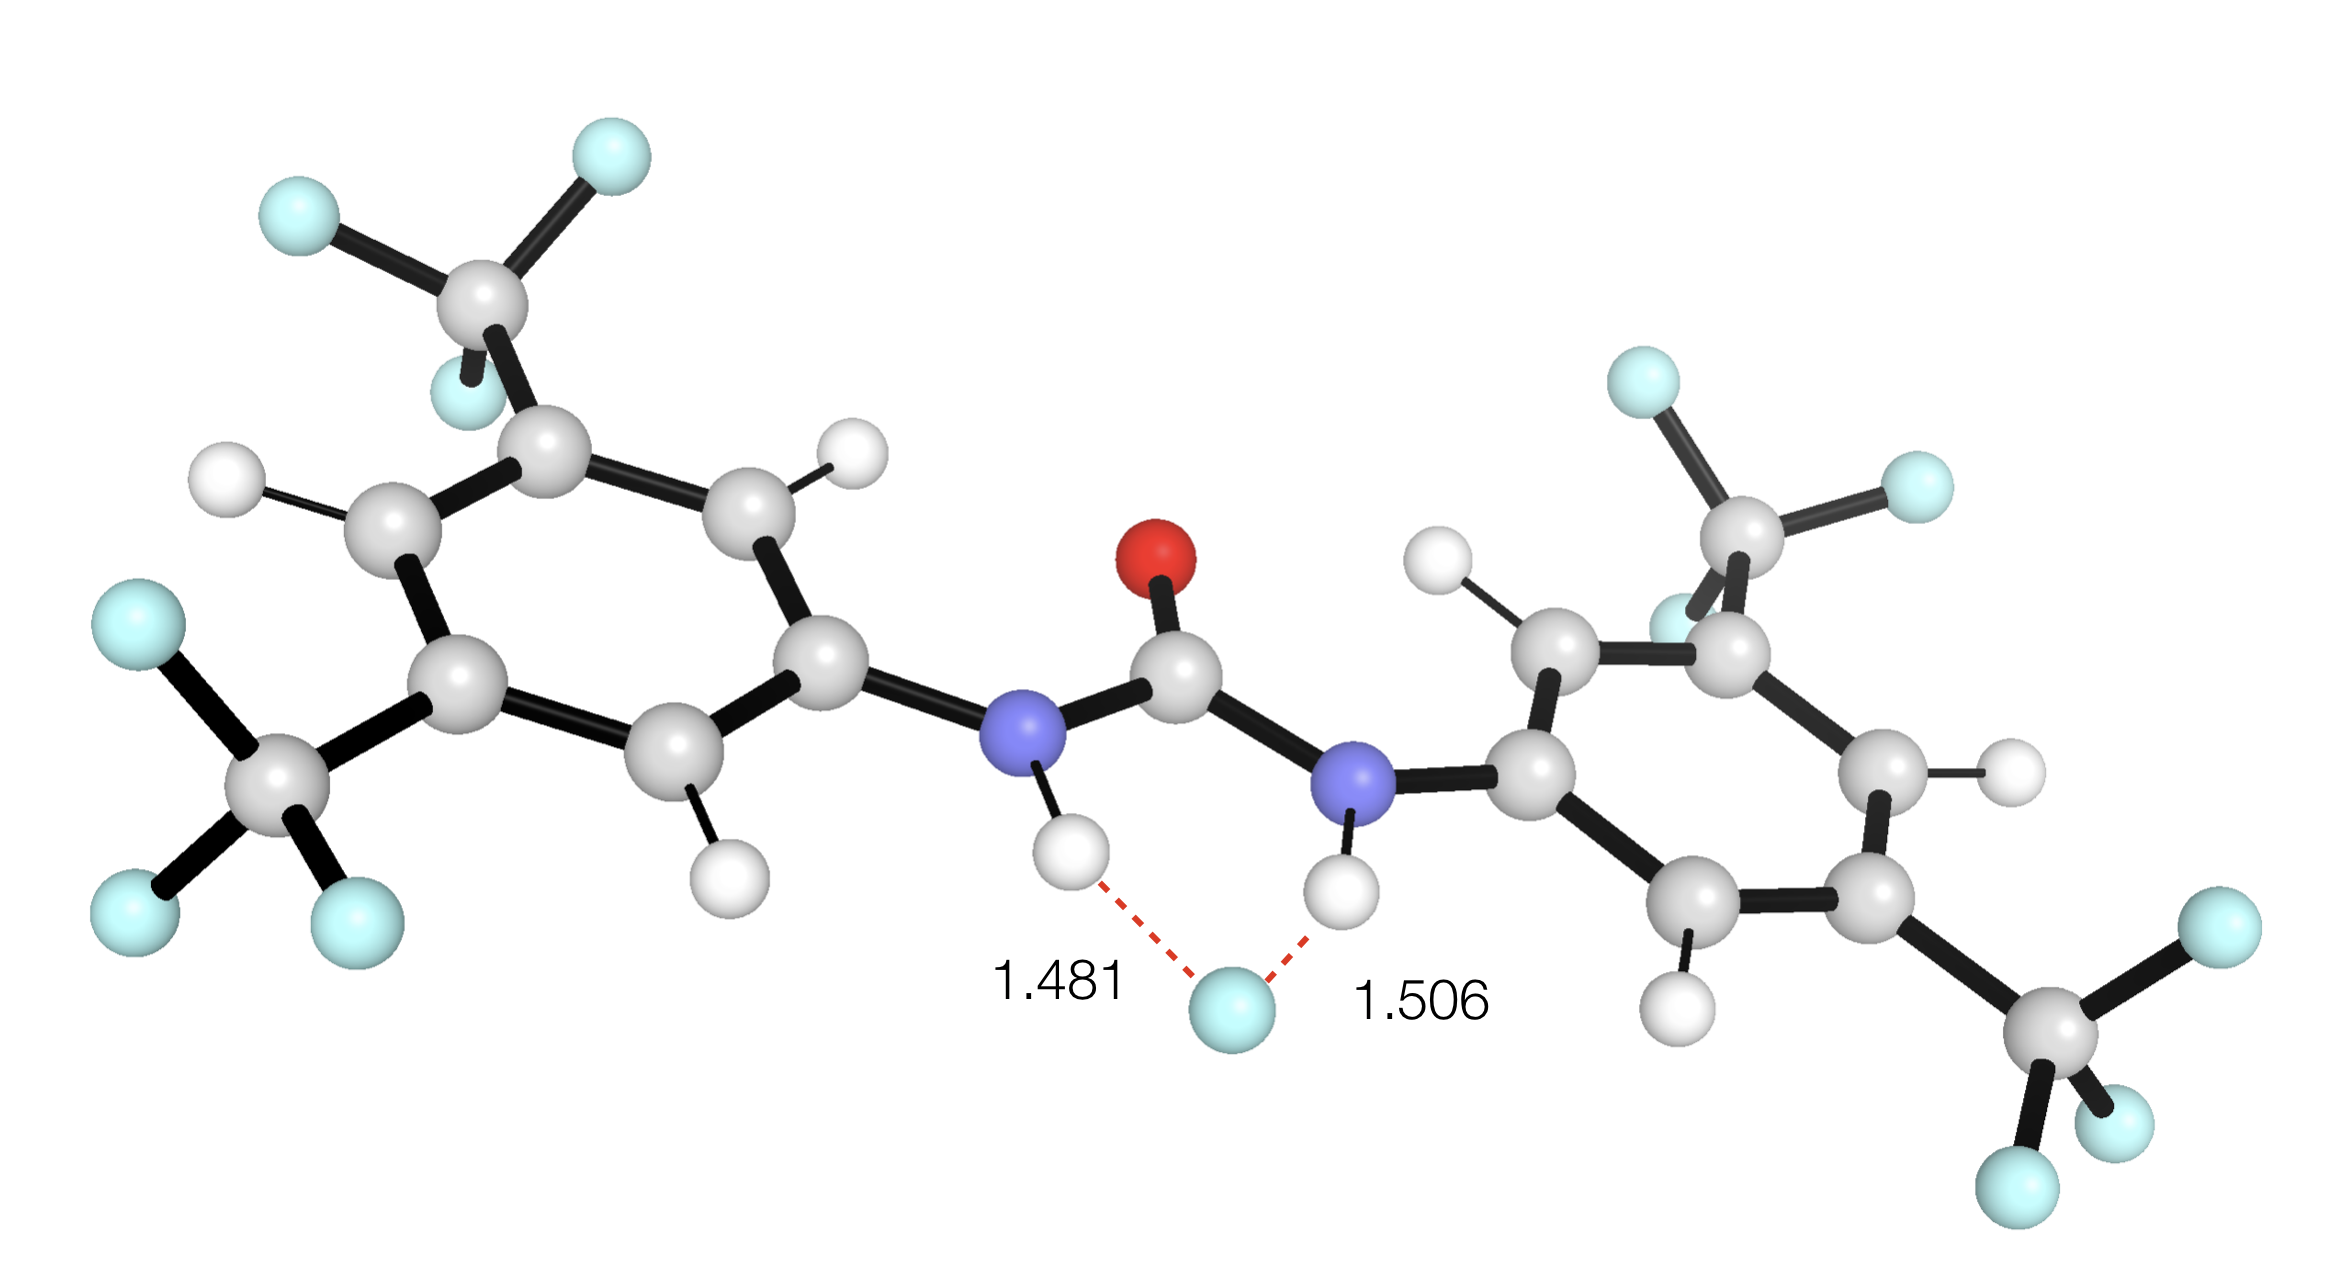
\includegraphics[width=12cm]{5/autode/figs/figS12}
	\vspace{0.4cm}
	\hrule
	\caption{Most stable NCI complex conformer for a urea-fluoride hydrogen-bonding complex located using \ade at the XTB level. Distances shown in \AA. See full supporting information for the associated input script.}
	\label{fig::ade_si_12}
\end{figure}

\clearpage
\subsection{Algorithm Details}
\label{section::ade_si_algorithm}

To outline the algorithm in more detail than shown in the high-level workflow (Figure \ref{fig::ade_2}) for an S$_N$2 reaction (Figure \ref{fig::ade_5}, with the input reproduced below) the partial trace of function calls is shown and commented where the function is not self-explanatory, or there are multiple possibilities exist depending on the system. Note that this trace will likely change in development but is accurate for the 1.0.0a0 release. Only a single molecule initialization (MeCl), reaction initialization and calculating reaction profile functions calls are shown. Functions without a prefix (e.g. RDKit.) are \ade functions.
\\\\
\hrule
\code{MeCl = Reactant(name=`CH3Cl', smiles=`ClC')}
\hrule

\begin{enumerate}
	\item \code{init_smiles(`ClC')}.
	
	\begin{enumerate}
		\item \code{any(metal in smiles for metal in metals)} $\rightarrow$ False.\\
		If true then use the RB algorithm to generate 3D 
		structure.
		
		\item \code{init_organic_smiles(‘ClC’)}
		
		\begin{enumerate}
			\item \code{rdkit.Chem.MolFromSmiles(‘ClC’)}
			
			\item \code{rdkit.Chem.AddHs(..)}
			
			\item \code{rdkit.AllChem.EmbedMultipleConfs(..)}
			
			\item  \code{make_graph(..)}
			Add nodes and edges from the atoms and RDKit
			bonds defined by the SMILES connectivity, set 
			stereocenters inc. Z/E alkenes.
			
			\item \code{are_coords_reasonable} $\rightarrow$ True
			If the coordinates aren’t reasonable then revert to
			RB algorithm to generate a 3D structure.
			
			\item  \code{check_bonds(..)}
			If the connectivity based on the 3D geometry 
			defined by distances is different to the SMILES         
			connectivity display an error.
		\end{enumerate}
	\end{enumerate}	
\end{enumerate}

\vspace{0.5cm}

\hrule
\code{reaction = Reaction(Flouride, MeCl, Chloride, MeF, name=`sn2', solvent_name=`water')}

\hrule


\begin{enumerate}
	\item \code{classify(..)}
	Classify the reaction based on the number of
	reactants and products. If there are no reactants/ 
	products throw an exception.
	
	\item \code{get_solvent(solvent_name)}
	
     \item \code{_check_solvent()}
	If the reactant and product molecules that comprise
	this reaction have an associated solvent this        
	function checks they match. Also permissible for
	all molecule.solvent = None for a reaction in the
	gas phase.
	
	\item \code{_check_balance()}
	Ensure that the number of atoms and the total
	charge are conserved reactants $\rightarrow$ products,       
	otherwise throw an exception. 
\end{enumerate}

\vspace{0.5cm}
\hrule
\code{calculate_reaction_profile()}
\hrule

\begin{enumerate}
	\item  \code{find_lowest_energy_conformers()}
	
	\begin{enumerate}
		\item \code{for mol in reacs + prods: mol.find_lowest_energy_conformer()}
	
		\begin{enumerate}
			\item \code{_generate_conformers()}
			If RDKit conformers are fine then use the
			ETKDGv2() algorithm to generate 
			conformers with a specified RMSD and
			max number cutoff. Otherwise use the RB
			algorithm with the same cutoffs. Both 
			are parallelized.
			
			\item \code{for conf in mol.conformers: conf.optimise(lmethod)}
			Initially optimise all conformers at the
			low-level method with keywords.opt to
			generate structures (hopefully) closer to
			the minima on the high-level method 
			surface
			
			\item \code{for conf in mol.conformers: conf.optimise(hmethod)}
			Failures in Gaussian internal coordinate
			bends are corrected by running a few
			optimisation steps in Cartesian
			coordinates then switching back to
			internals .
			
			\item \code{_set_lowest_energy_conformer()}
			Enumerate all the conformers in this
			molecule and set mol.atoms, mol.energy
			as the conformer with the lowest energy
			that is also graph isomorphic to the
			molecule’s graph to remove any 
			structures with different connectivity i.e.
			not conformers.
		\end{enumerate}
	\end{enumerate}
	
	\item \code{optimise_reacs_prods()}
	\begin{enumerate}
		\item \code{for mol in reacs + prods: mol.optimise(hmethod)}
		Optimise the geometry with the high-level method
		but don’t reset the molecular graph
	\end{enumerate}
	
	\item \code{find_complexes()}
	
	\begin{enumerate}
		\item \code{ReactantComplex(reacs, ..)}
		\begin{enumerate}
			\item \code{charge = sum(reacs.charge)} $\rightarrow -1$
			\item \code{mult = sum(reacs.mult) - (n-1)} $\rightarrow$ 1
			Spin multiplicity is the sum of the two where n is 
			the number of reactants by default.
			atoms = reacs.atoms
			\item \code{solvent = reacs[0].solvent} $\rightarrow$ water
			\item \code{graph = union(reacs.graph)}
		\end{enumerate}
		
		\item \code{ProductComplex(prods, ..)}
		As for reactant complex.
	\end{enumerate}
	
	
	\item \code{locate_transition_state()}
	\begin{enumerate}
		\item $b_R > b_P \rightarrow$ False.\\ 
		If True then call \code{switch_reacs_prods()},
		then switch back after locating TSs.
		
		\item \code{find_tss()}
		Locate all possible transition states for this R $\rightarrow$ P
		rearrangement.
		
		\begin{enumerate}
			\item \code{species_are_isomorphic(reac, prod)} $\rightarrow$ False.\\
			If the graphs of reactant and product $(R, P)$ are
			isomorphic then the bond rearrangement of
			interest is not obvious and this returns true and
			\code{find_tss} returns None.
			
			\item \code{get_bond_rearrs(reac, prod, ..)}
			Get all possible bond rearrangements that generate an R’ that is isomorphic to P.
			
			\item \code{bond_rearrs is None} $\rightarrow$ False.\\
			If a set of bond rearrangements cannot be found then \code{find_tss} returns None.
			
			\item \code{for g in bond_rearrs:}
			Attempt to locate a TS for all possible bond rearrangements (g). 
			
			\item \code{translate_rotate_reactant()}
			
			\item \code{reoder_product_complex(..)}
			Reorder the atoms in the product complex using
			the atom mapping from $R’$ to $P$ so $R$ and $P$ have
			atoms that map.
			
			\item \code{is_worth_truncating(..)} $\rightarrow$ False.\\
			Form the truncated reactant complex by
			swapping fragments for hydrogen if they are
			far enough away from the active atoms, then
			calculation the difference in number of atoms
			between the full complex and the truncated, if          
			$> 10$ then use the truncated complex then
			revert.
			
			\item \code{for ts_func in funcs()}:
			Enumerate possible TS guess functions, here a
			2D low-level scan, 1D breaking-bond scan and
			1D high-level forming bond scan in sequence
			until either there are no more functions or a
			TS has been found.
			
			\item \code{ts_guess = ts_func(reaction, ..)}
			Use the function to generate a transition state guess geometry as, in the first instance, the saddle point in the 1D/2D surface.
			
			\item \code{could_have_correct_mode(ts_guess)} $\rightarrow$ True.\\
			The ‘lowest’ mode in the Hessian must be negative (imaginary), be $|\nu| > 45 \text{ cm}^{-1}$, and has a contribution from the active atoms. The latter is defined by the mass weighted $|\nu_i|$ for an active atom $i$ being above a threshold. 
			
			
			\item \code{ts.optimise()}
			Use the TS optimiser in the high-level method to optimise to a first order saddle point. If there is $>1$ imaginary frequency following the successful termination displace along the spurious mode forwards and backwards to try and remove it. 
			
			\item \code{is_true_ts()}
			Check that the forward/reverse displacement leads to the expected change in active bond lengths (all $\Delta r$ $> 0.3$ \AA) or that displacement forwards and backwards along the largest magnitude imaginary mode leads to a structure that has a graph which is isomorphic to either the reactant complex or an optimised conformer of the reactant complex.
			
			\item \code{ts.save_template()}
			If \code{Config.make_ts_template}
			then save a TS template containing the
			atoms, distances, charge, multiplicity and
			solvent for subsequent use.
			
			\item \code{len(tss) == 0} $\rightarrow$ False.\\
			If no transition states can be found then \code{find_tss} returns None.
		\end{enumerate}
		
		\item \code{find_lowest_energy_ts()}
		If there is more than one TS that leads to products
		then choose the lowest energy.
		
	\end{enumerate}
	
	\item \code{find_lowest_energy_ts_conformer()}
	Use the repulsion + bonded force field to randomise
	coordinates then minimize using the low-level method
	with fixed active bond lengths, removing the similar
	based on RMSD and energy tolerance then reoptimising.
	at the high-level method from which a TS optimisation is
	run from the lowest energy. If this is both a ‘good’ TS
	and is lower energy than previously found then use this
	TS.
	
	\item \code{calculate_single_points()}
	\begin{enumerate}
		\item \code{for mol in reacs + prods: mol.single_point()}
	\end{enumerate}
	
	\item \code{plot_reaction_profile(..)}
	Spline between the points in the profile and optimise the
	points in the spline to generate stationary points at the
	minima/maxima for a smooth profile.

\end{enumerate}

In checking if the largest magnitude imaginary mode afforded by a Hessian calculation on the transition state guess geometry could be the ‘correct’ transition state mode that separates reactants and products there has to be a ‘significant contribution’ from the active atoms before a transition state optimization is performed. The significance is quantified by $d > 0.1$ based on empirical experience. Further \ade developments will introduce a more robust and interpretable measure where,


\begin{equation}
	d = \frac{\sum_{i \in \text{active}} w_i}{\sum_{i \in \text{atoms}} w_i} \quad,\quad w_i = \frac{M_i}{c_M} + 10 \frac{|\boldsymbol{v}_\text{imag}(i)|}{c_d}
\end{equation}

$M_i$ is the mass of atom $i$, $c_M$ = 1 amu, $v_\text{imag}(i)$ the normal mode displacement vector and $c_d = 1$ \AA. 


\begin{figure}[h!]
	\vspace{0.4cm}
	\centering
	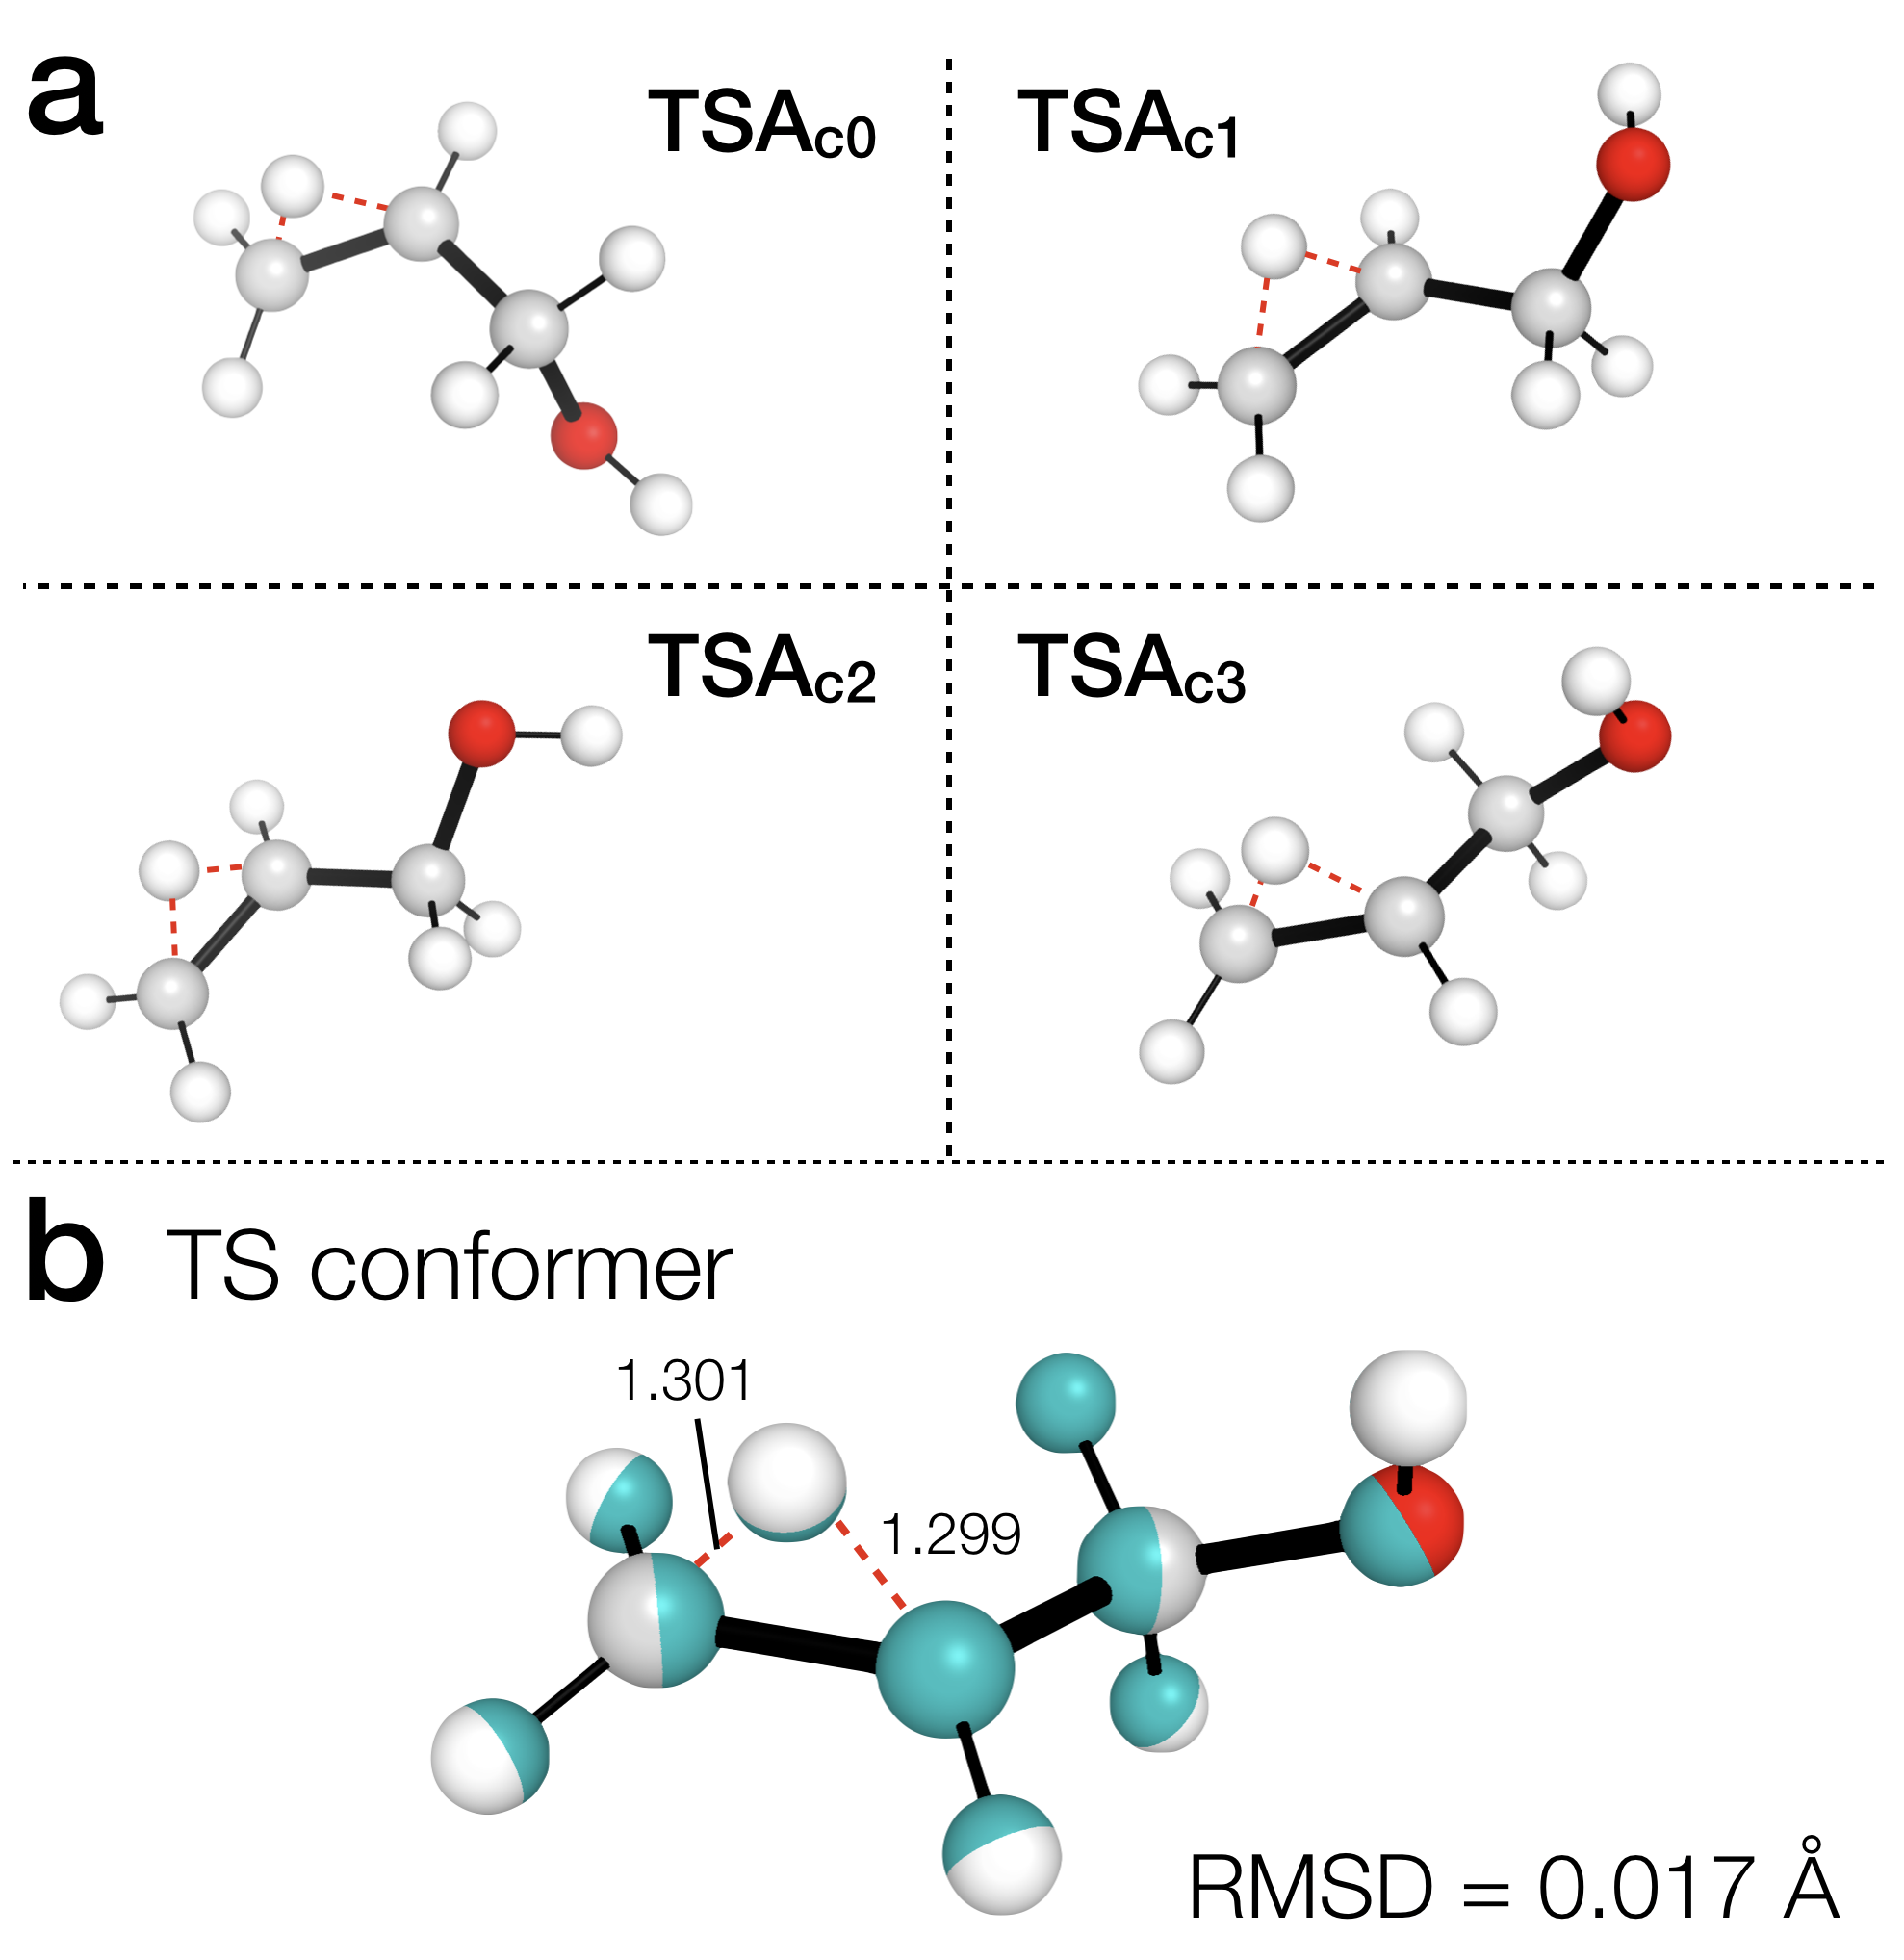
\includegraphics[width=9cm]{5/autode/figs/figS13}
	\vspace{0.4cm}
	\hrule
	\caption{H-migration reaction involved in the radical decomposition of 1-propanol. (a) Transition state analogue (TSA) conformers located with \ade and ranked in increasing energy (c0-c3)(b) optimised TS, starting from TSAC1 conformer, at PBE0-D3BJ/def2-SVP compared to the lowest energy TS conformer reported in ref. \cite{Ferro-Costas2018} (cyan). RMSD calculation include all atoms. Key distances quoted in \AA.}
	\label{fig::ade_si_13}
\end{figure}



\begin{figure}[h!]
	\vspace{0.4cm}
	\centering
	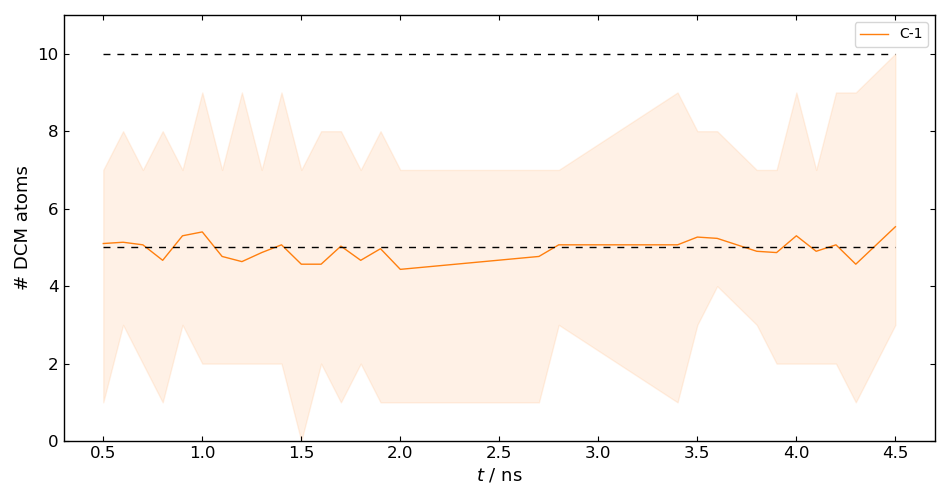
\includegraphics[width=14.5cm]{5/autode/figs/figS14.pdf}
	\vspace{0.4cm}
	\hrule
	\caption{Most stable intermediates and transition states for the Ireland-Claisen reaction profile shown in Figure \ref{fig::ade_7} located by \ade at the B3LYP-D3BJ/6-31G(d) level of theory using ORCA/XTB. }
	\label{fig::ade_si_14}
\end{figure}



\begin{figure}[h!]
	\vspace{0.4cm}
	\centering
	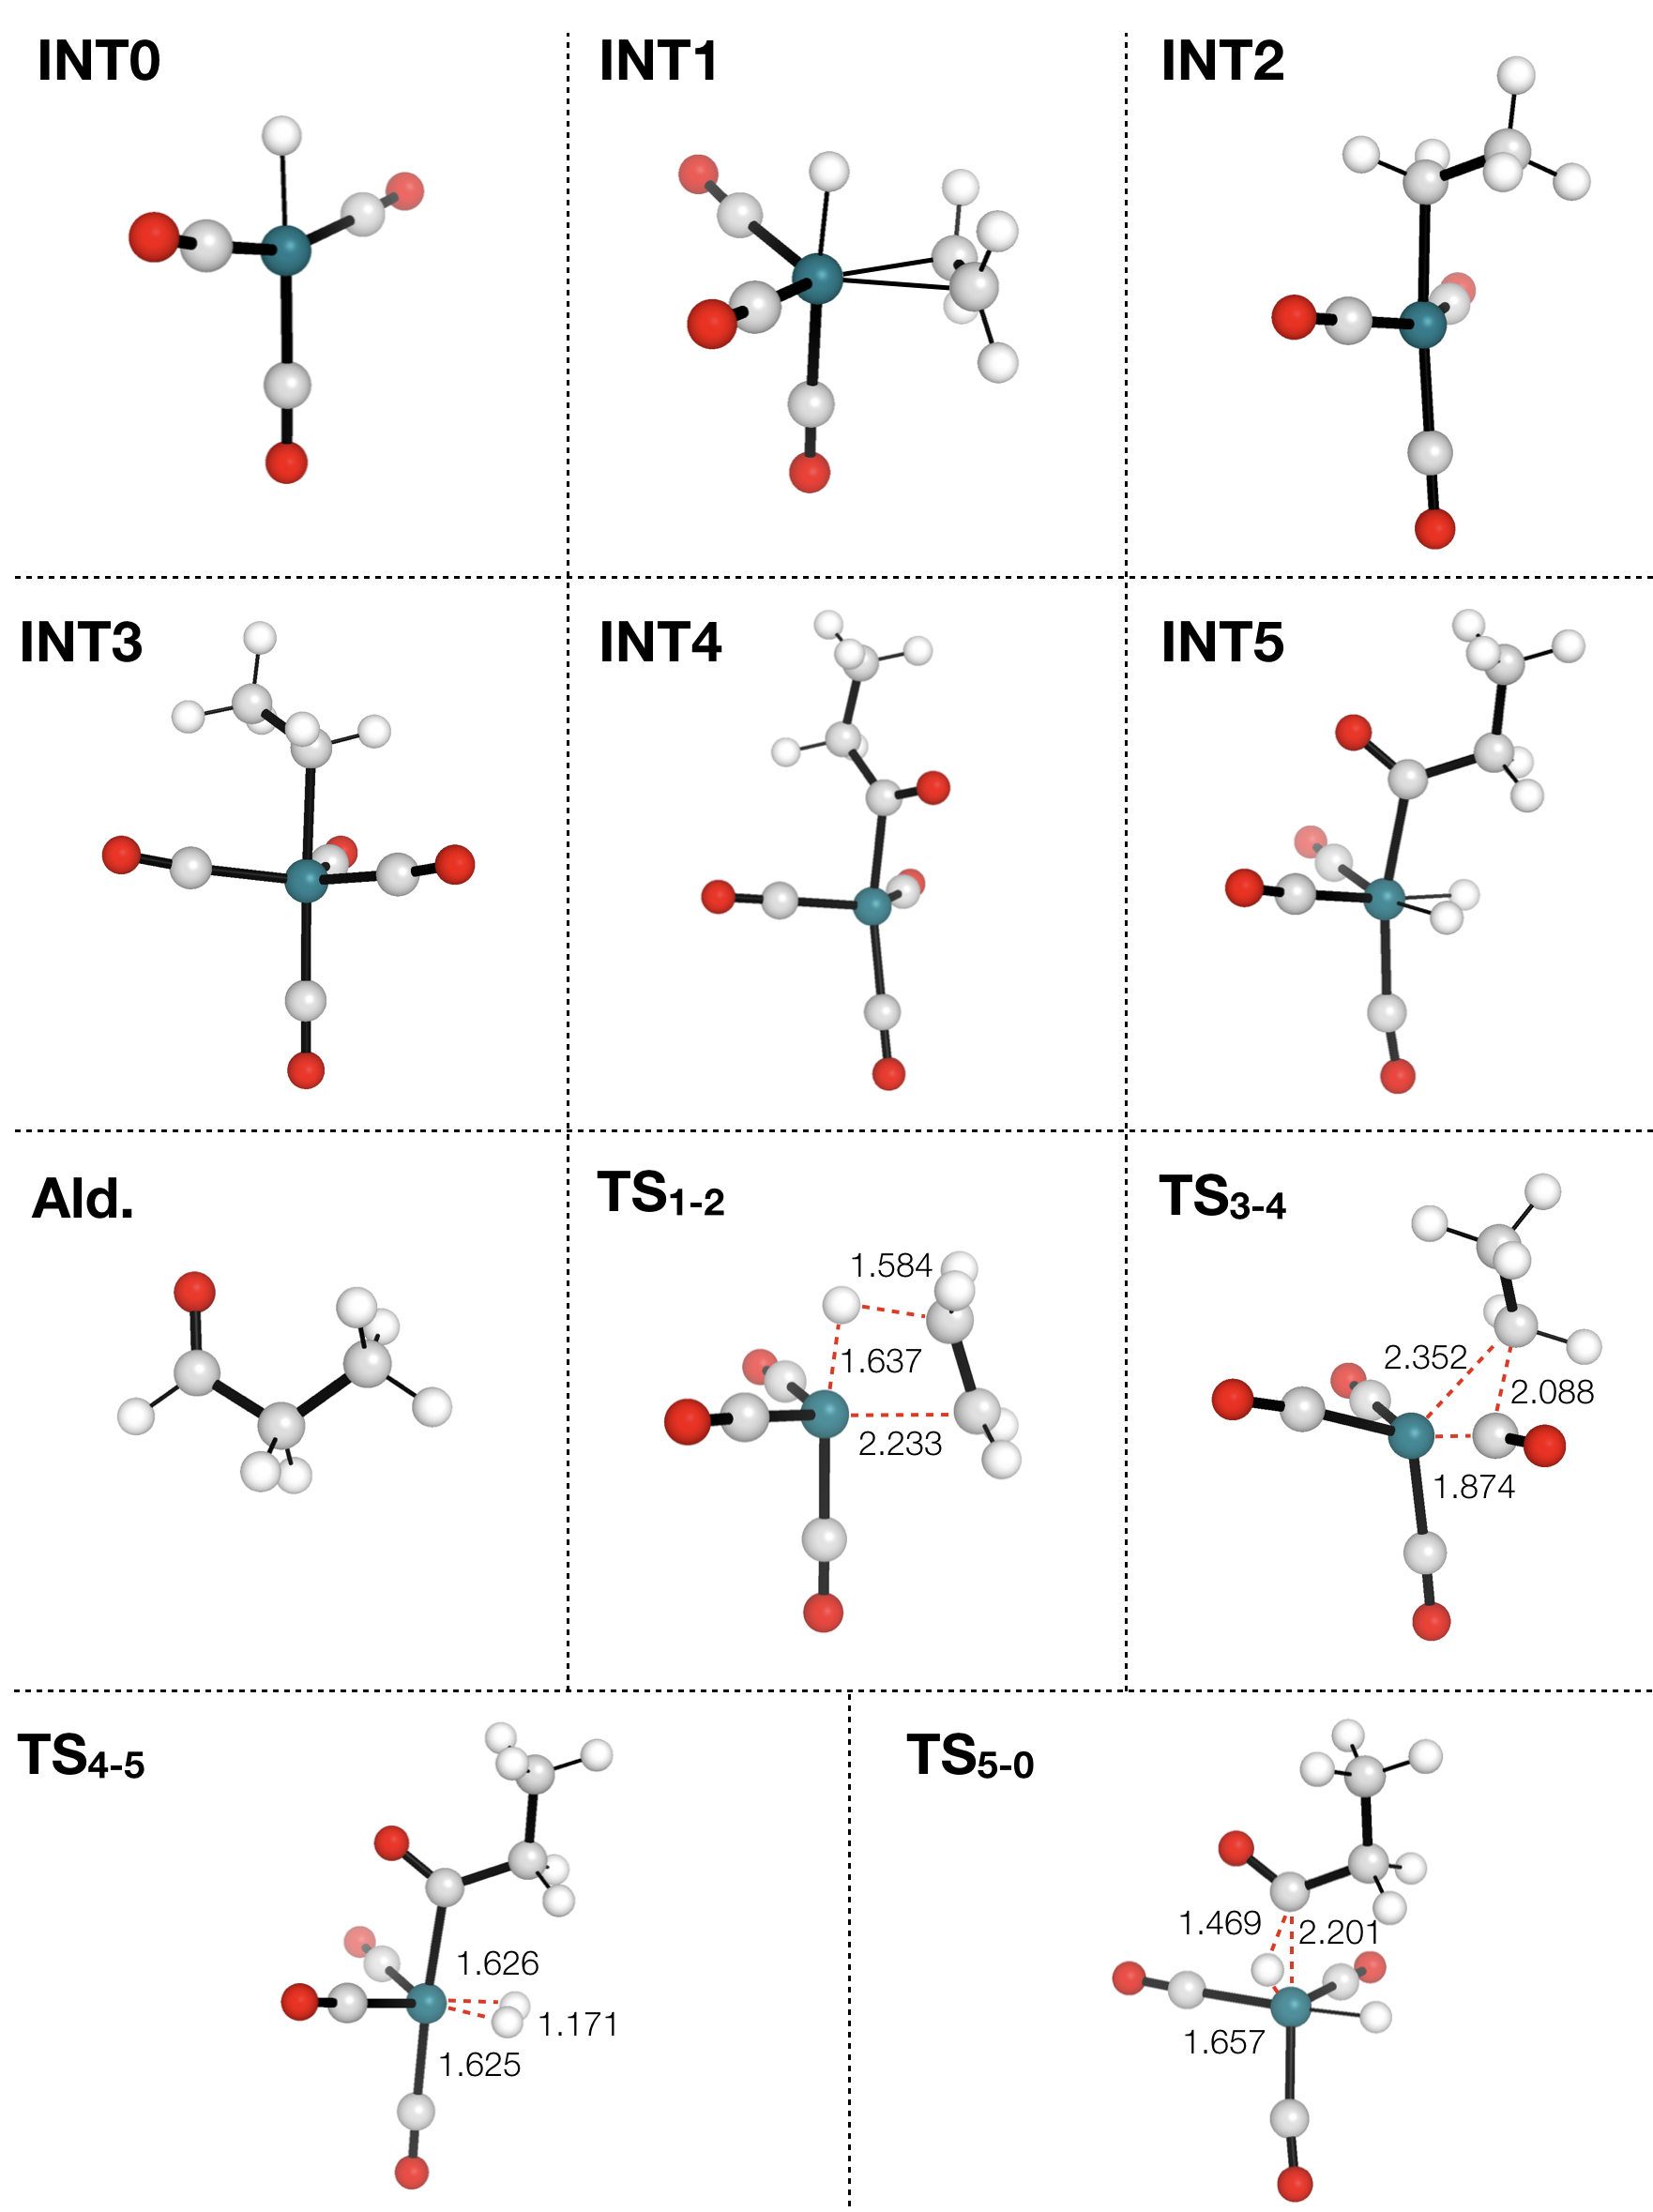
\includegraphics[width=13cm]{5/autode/figs/figS15}
	\vspace{0.2cm}
	\hrule
	\caption{Most stable intermediates and transition states for the Heck-Breslow mechanism of hydroformylation shown in Figure \ref{fig::ade_8} located by \ade at the PBE-D3BJ/def2-SVP level of theory.}
	\label{fig::ade_si_15}
\end{figure}



\begin{figure}[h!]
	\vspace{0.4cm}
	\centering
	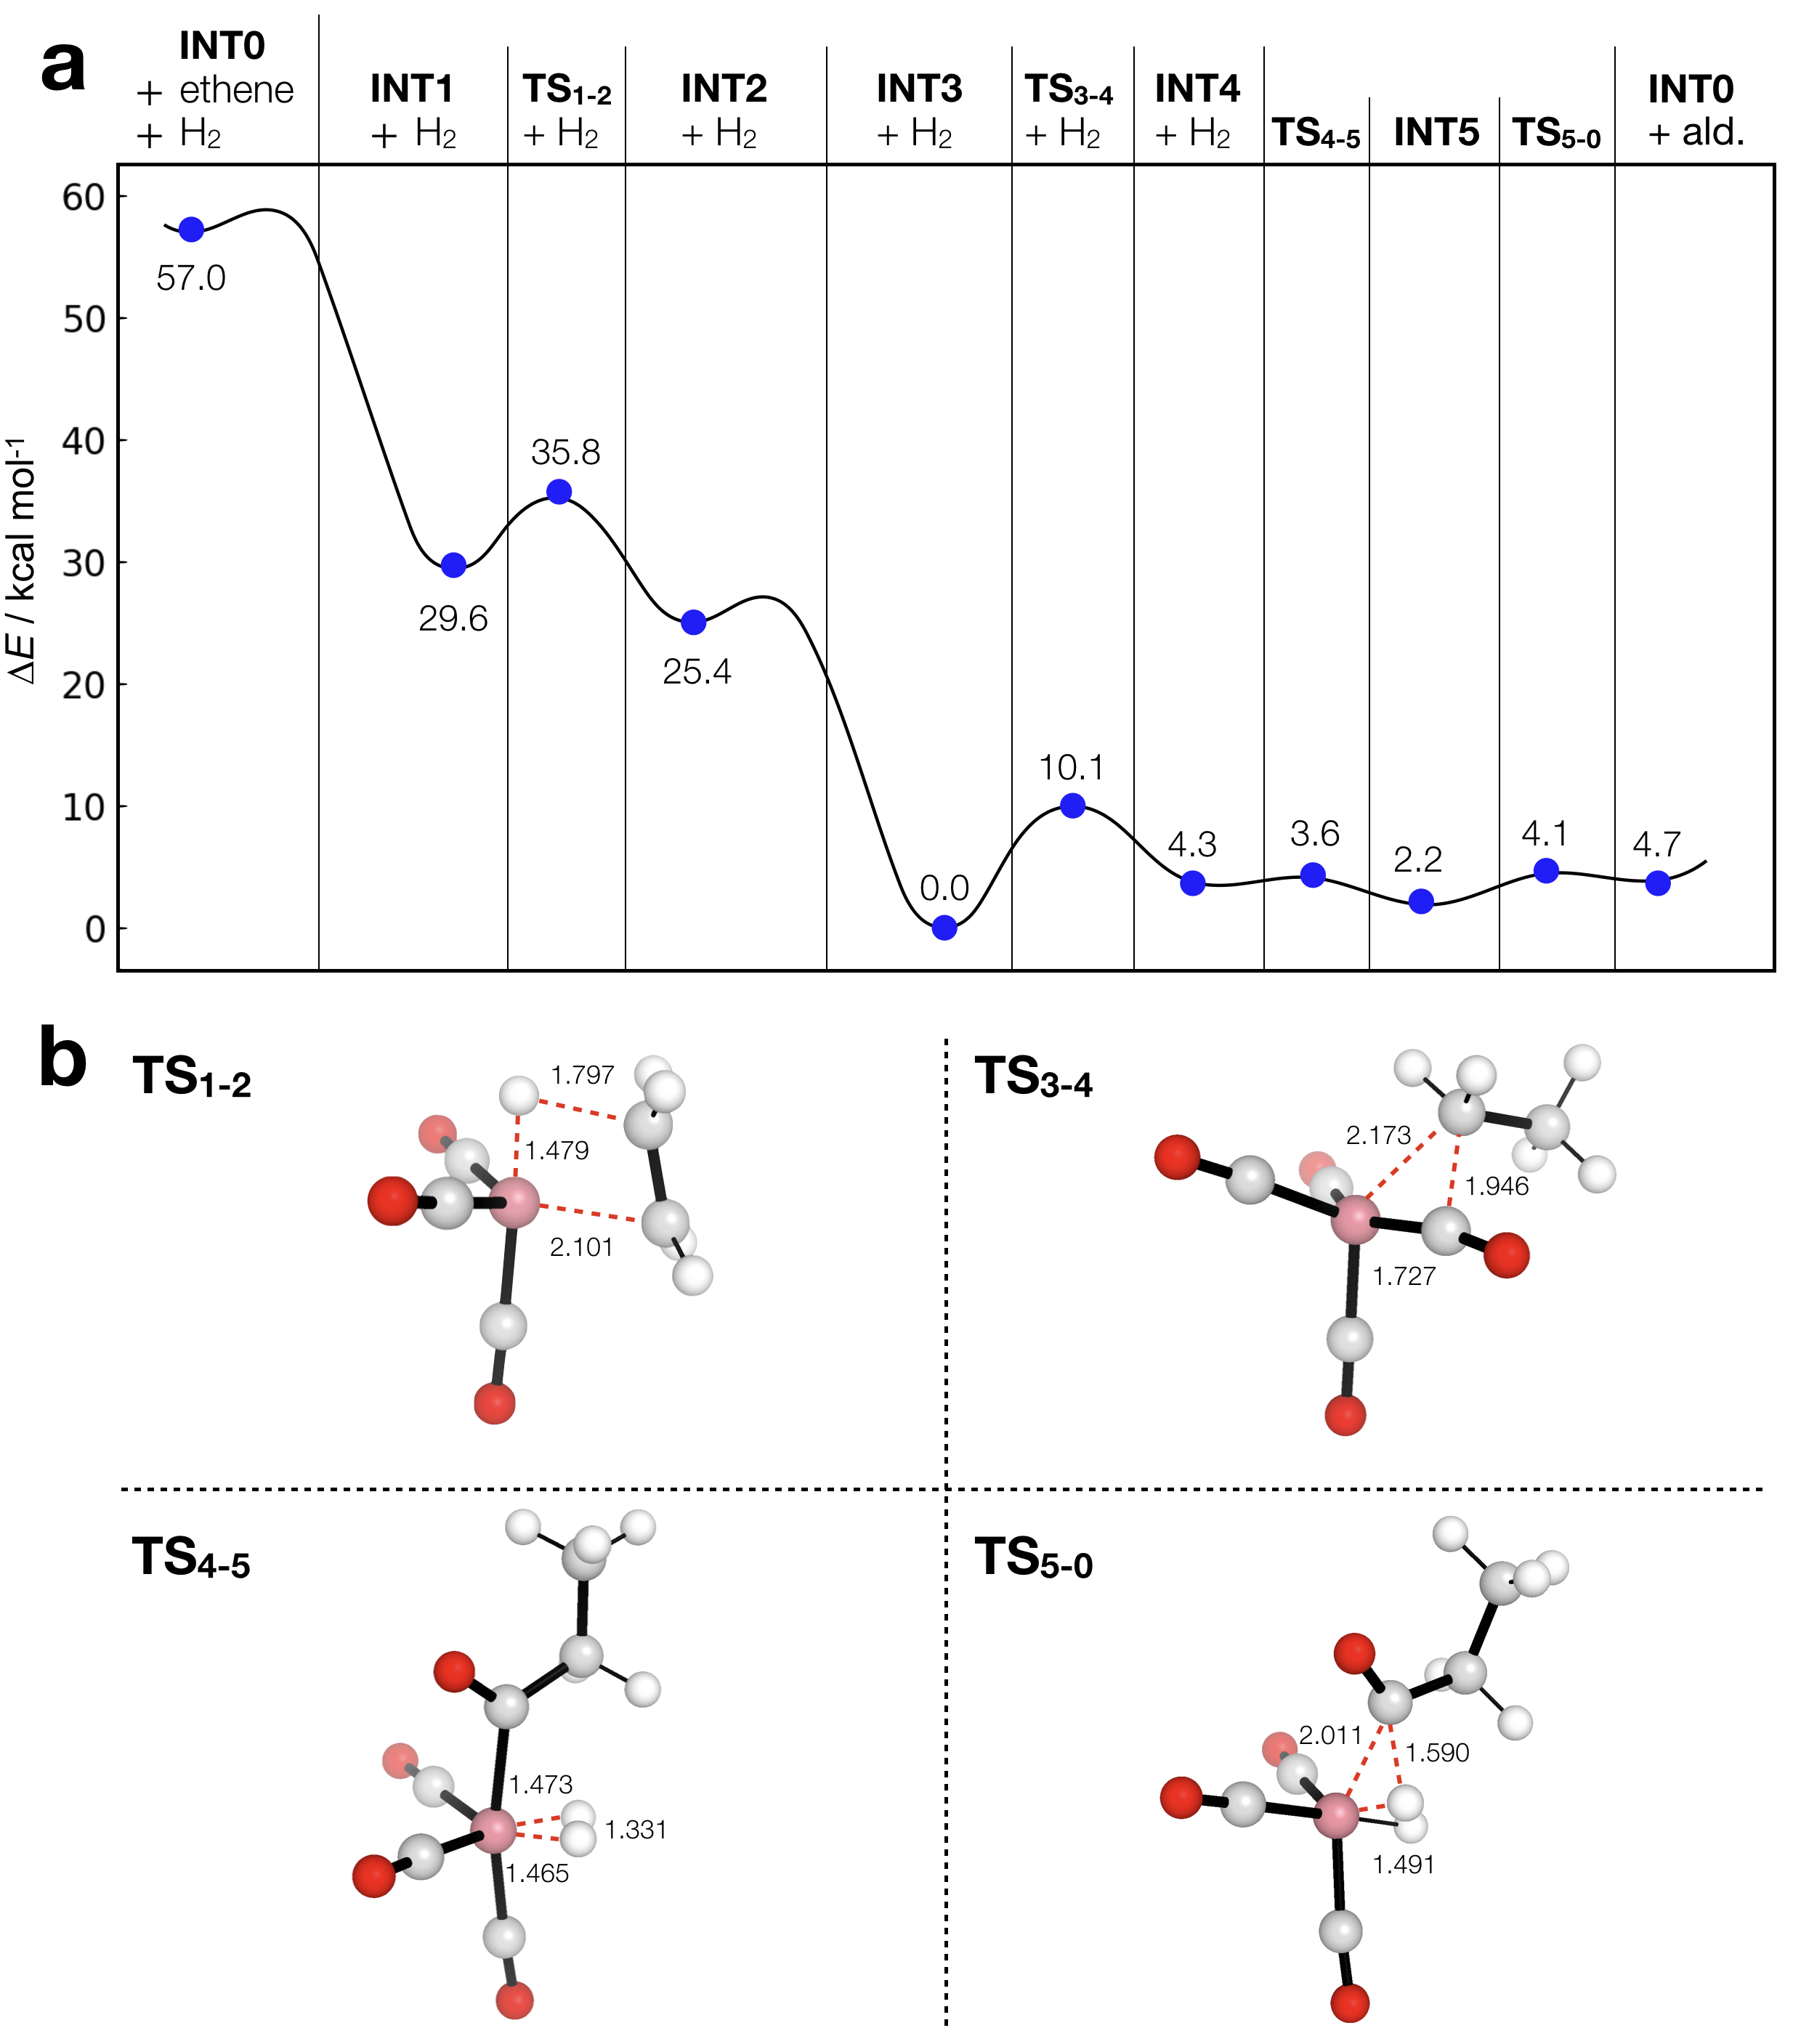
\includegraphics[width=15cm]{5/autode/figs/figS16}
	\vspace{0.2cm}
	\hrule
	\caption{Co-catalyzed hydroformylation (a) reaction profile and (b) transition state geometries generated in \ade (ORCA/XTB, PBE0-D3BJ/def2-TZVP//PBE0-D3BJ/def2-SVP). ald. = propionaldehyde. TS${}_{5-0}$ is not a local maximum due to basis set superposition error making the TS more stable than the separated aldehyde and INT0. Electronically barrierless ligand association TSs are not calculated.}
	\label{fig::ade_si_16}
\end{figure}


\begin{figure}[h!]
	\vspace{0.4cm}
	\centering
	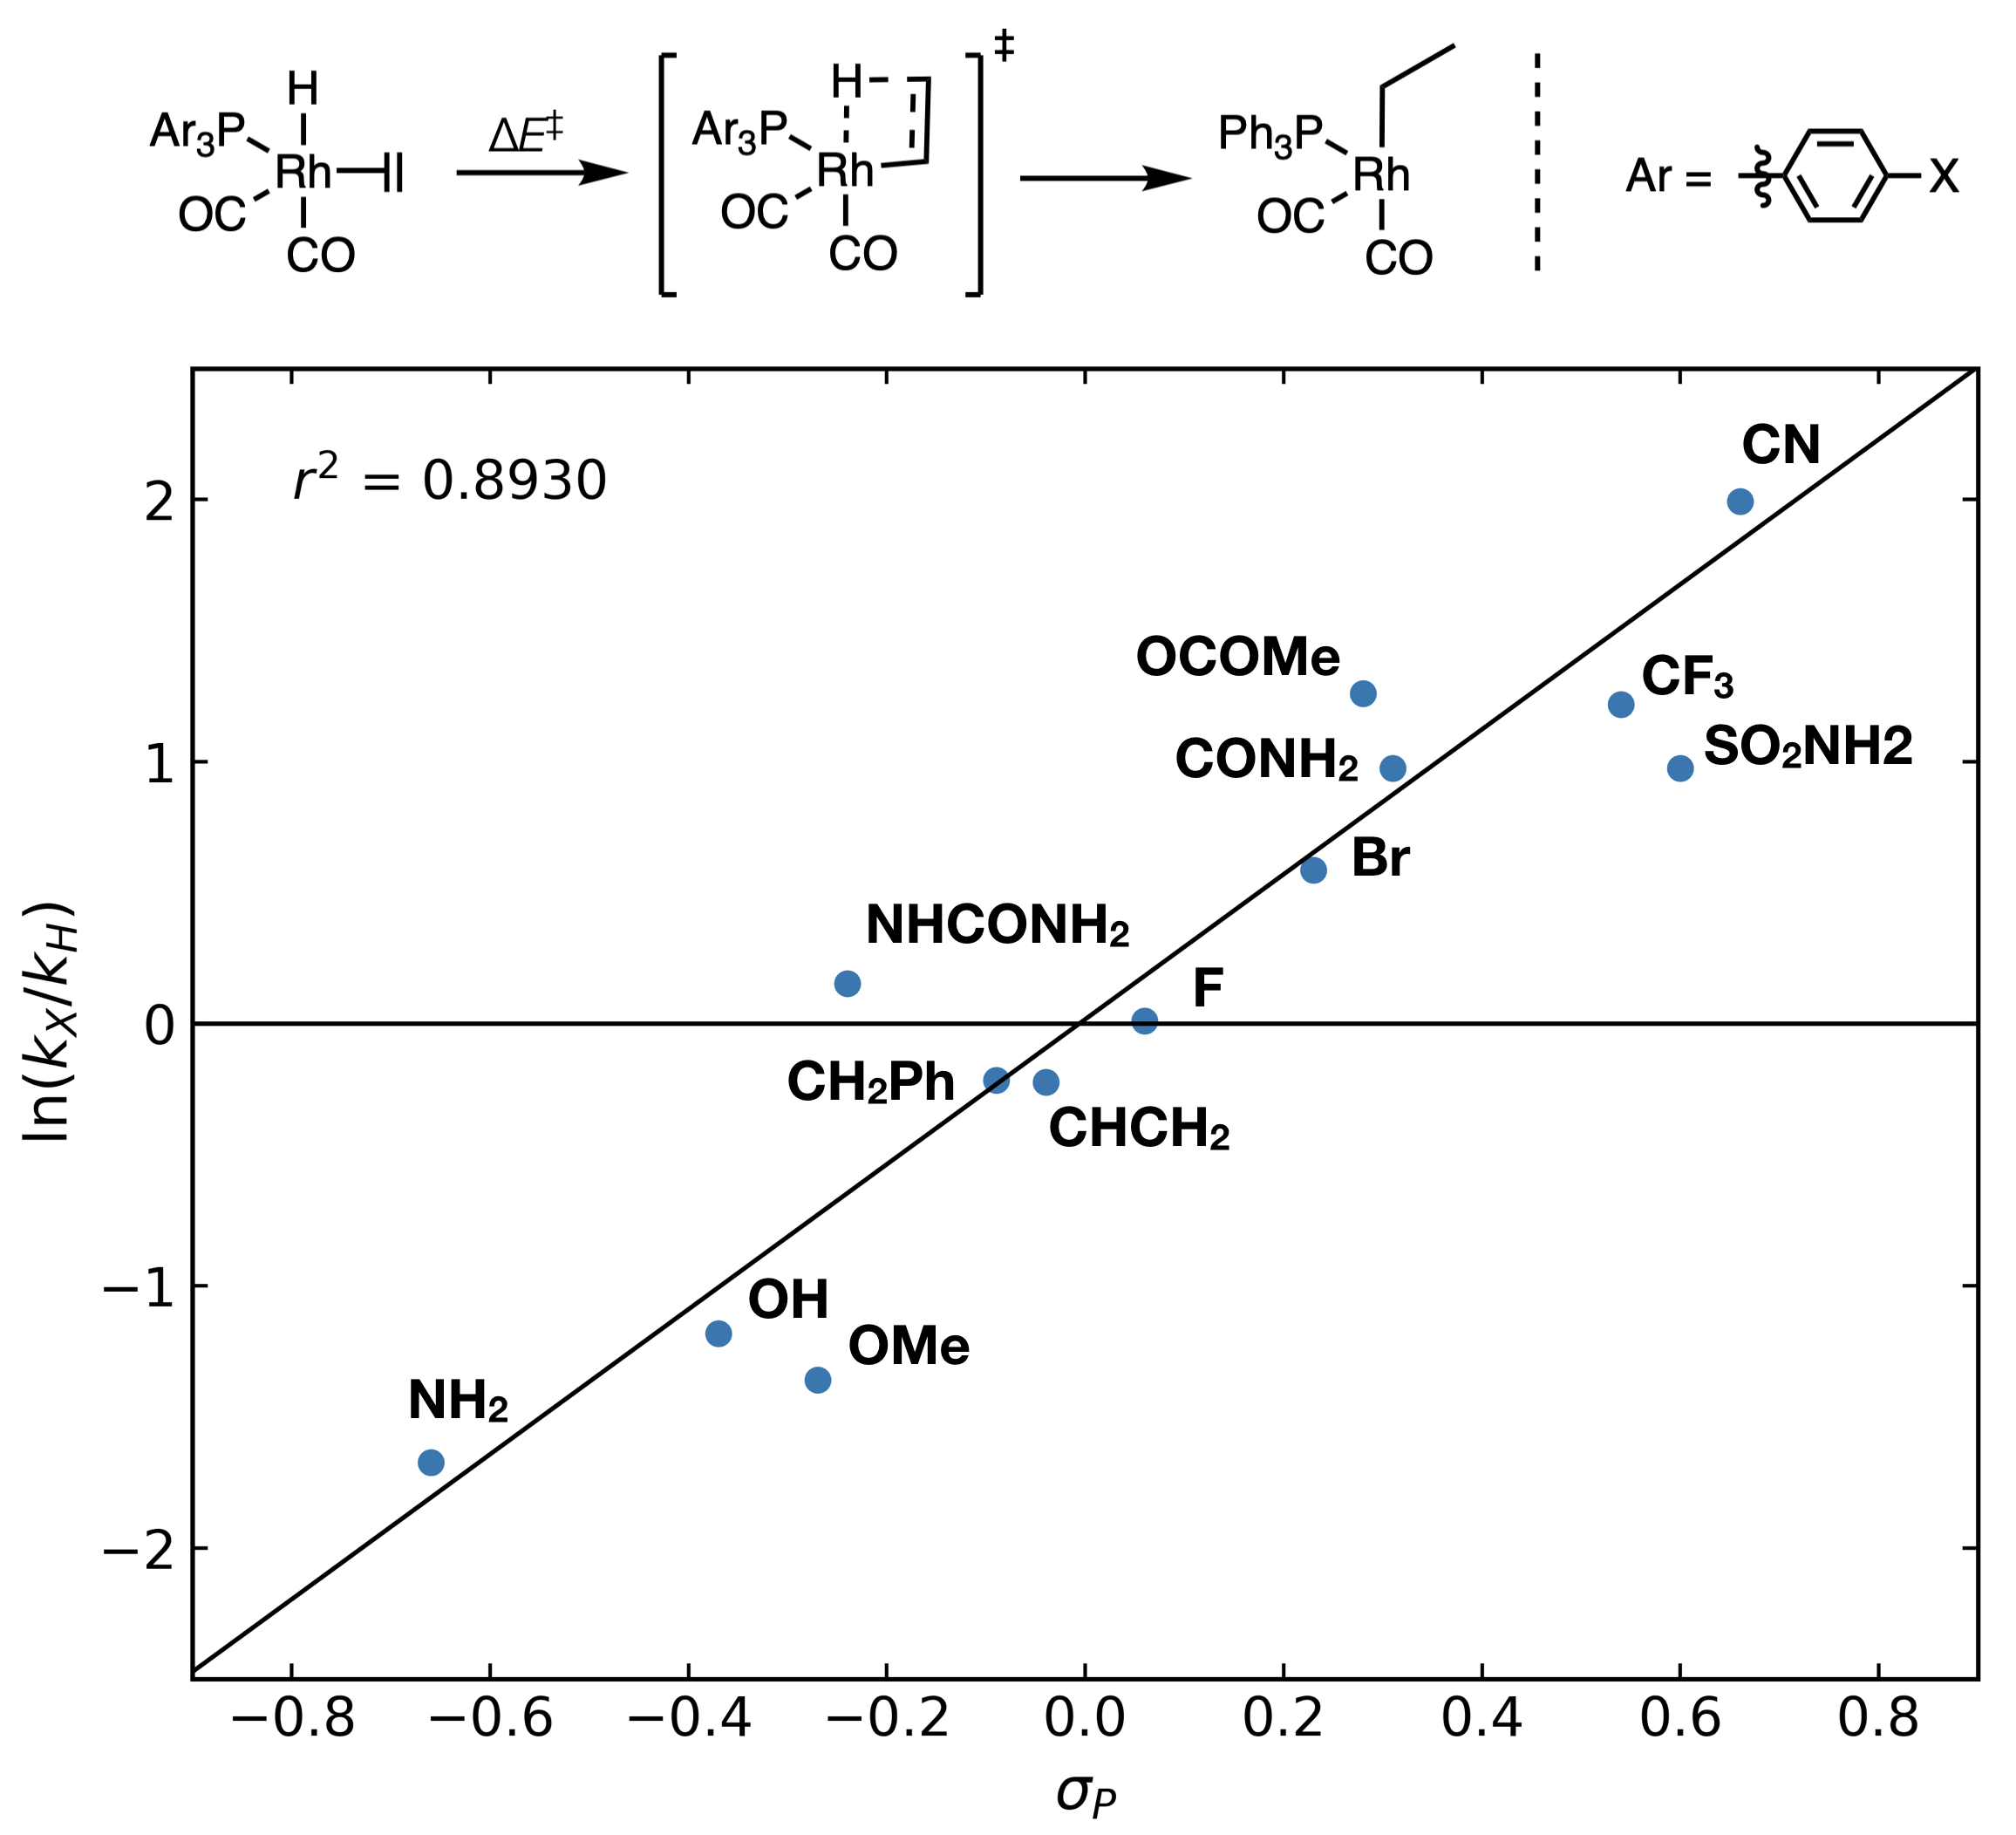
\includegraphics[width=11cm]{5/autode/figs/figS17}
	\vspace{0.2cm}
	\hrule
	\caption{Relative rate ($\ln(k_X/k_H) \approx -\Delta\Delta E_A^\ddagger/RT$, T = 373.15 K) for the hydrogen migration catalysed by [RhH(CO)$_2$(PAr$_3$)(ethene)]. $\Delta\Delta E_A^\ddagger$ is the energy difference between the TS analogue and the canonical TS with X = H. The TS analogues are generated by keeping bonds fixed and only optimizing the added functional group). Energies calculated at PBE0-D3BJ/def2-SVP where Ar = $p$-C$_6$H$_5$X and X = $\{$H, F, Br, CF$_3$, CH=CH${}_2$, CONH$_2$, NO$_2$, NH$_2$$\}$.}
	\label{fig::ade_si_17}
\end{figure}


\clearpage
\subsection{Reaction Classes}

To demonstrate the applicability of \ade to multiple reaction classes we have generated reaction profiles for a selection of organic reaction types choosing a minimal example in each case (Figure \ref{fig::ade_si_18a}). Several reactions (Figure \ref{fig::ade_si_18a} g, i, j, k) which have a TS below either products or reactants due to less stable separated anionic components at the DFT method used. Of particular note is acylium addition to benzene (Figure \ref{fig::ade_si_17}), where our TS conformational search algorithm finds a true TS (that links reactants and products) that is more stable (0.7 \kcal) than the Wheland intermediate conformer obtained with RDKit (2.3 \kcal). These differences are within the error of the level of theory used and suggest that this reaction is electronically barrierless. 

All of the reaction profiles were generated successfully with the exception of the stepwise conversion of acetic acid to acetyl chloride by thionyl chloride, for which only the chloride addition TS was located with \ade (Step II, Scheme 1). This resulted from the substitution reaction being barrierless at the chosen \lmethodx (GFN2-XTB) and saddle point found on the 2D surface at the \code{low_opt} (PBE-D3BJ/ma-def2-SVP) level of theory not being a saddle point on the opt level (PBE0-D3BJ/ma-def2-SVP) surface. Note that \ade by default does not perform a 2D scan at the opt level due to computational expense. Both of these limitations are not intrinsic to the method, but rather of the accuracy electronic structure theory packages currently available.



\begin{figure}[h!]
	\vspace{0.4cm}
	\centering
	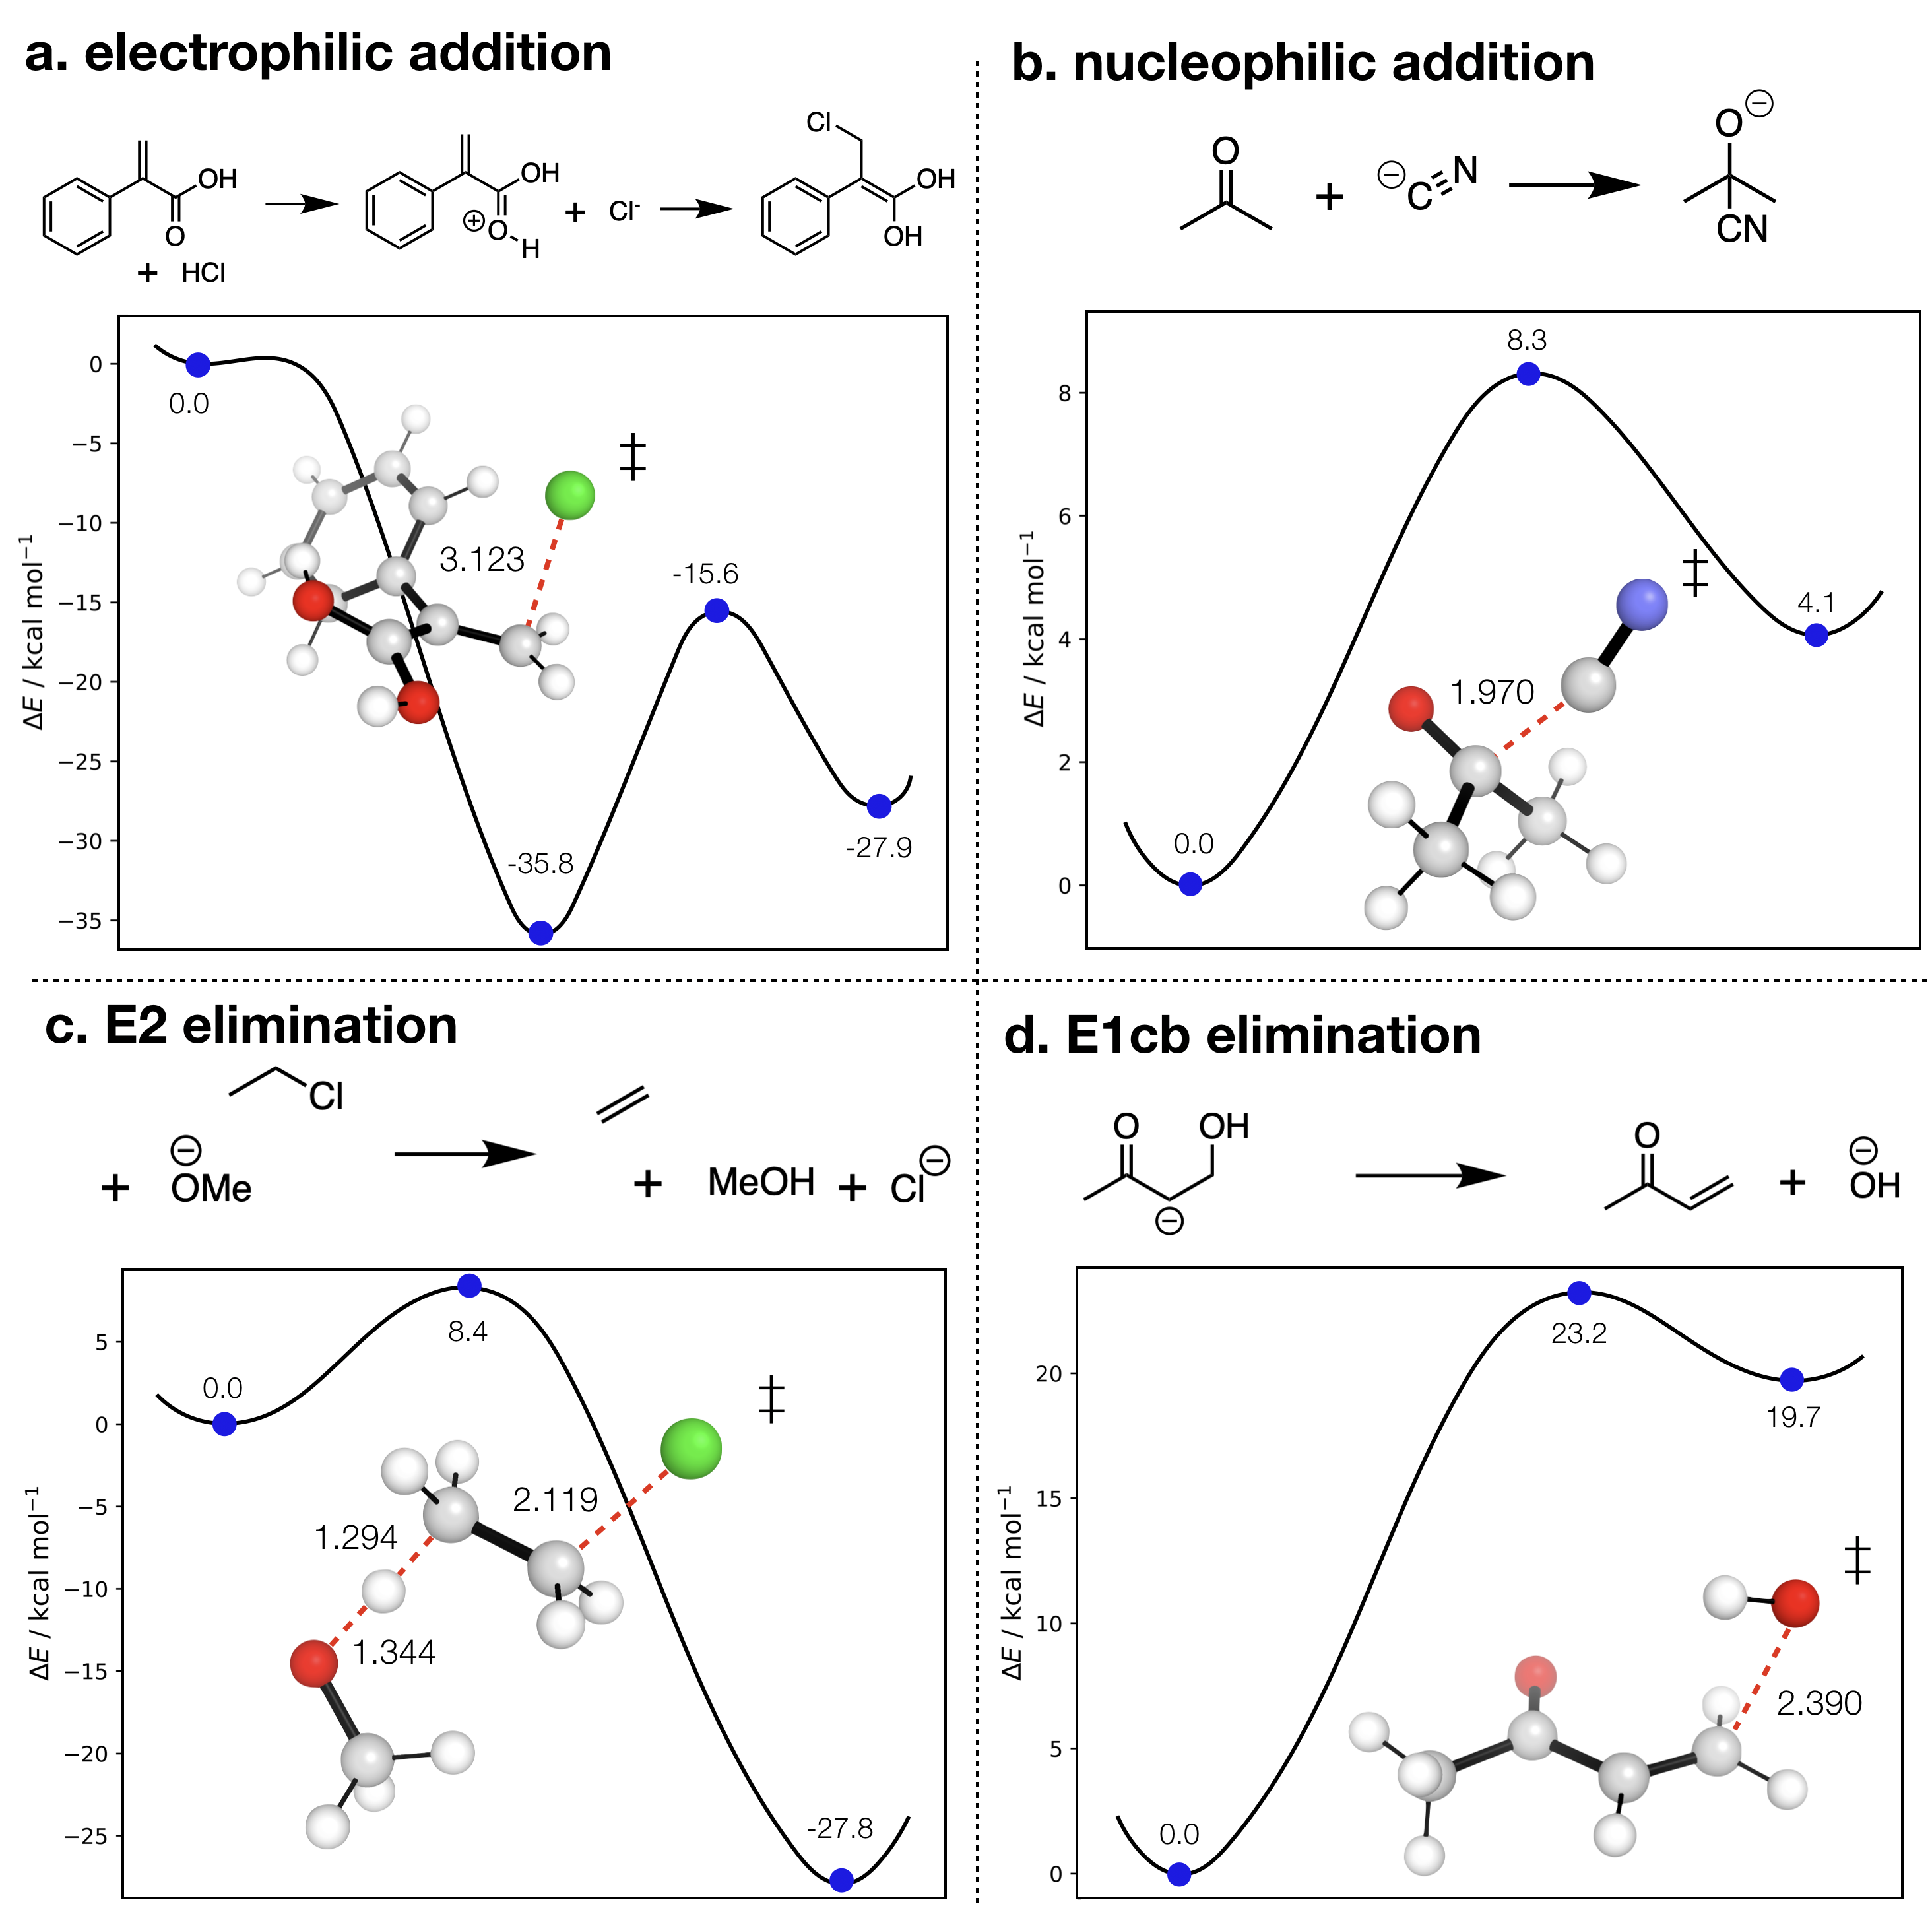
\includegraphics[width=\textwidth]{5/autode/figs/figS18a-d}
	\vspace{0.2cm}
	\hrule
	\caption{Reaction profiles for a range of organic reaction classes calculated at PBE0-D3BJ/def2-TZVP//PBE0-D3BJ/def2-SVP for neutral and CPCM(water)-PBE0-D3BJ/ma-def2-TZVP//CPCM(water)-PBE0-D3BJ/ma-def2-SVP for reactions with an anionic component with ORCA/XTB. (c) TS contained a second spurious imaginary frequency $< 50i \text{ cm}^{-1}$ that could not be removed via displacement along the imaginary vector. b. TS contained two spurious imaginary frequency $< 50i \text{ cm}^{-1}$. Distances quoted in \AA.}
	\label{fig::ade_si_18a}
\end{figure}

\begin{figure}[h!]
	\vspace{0.4cm}
	\centering
	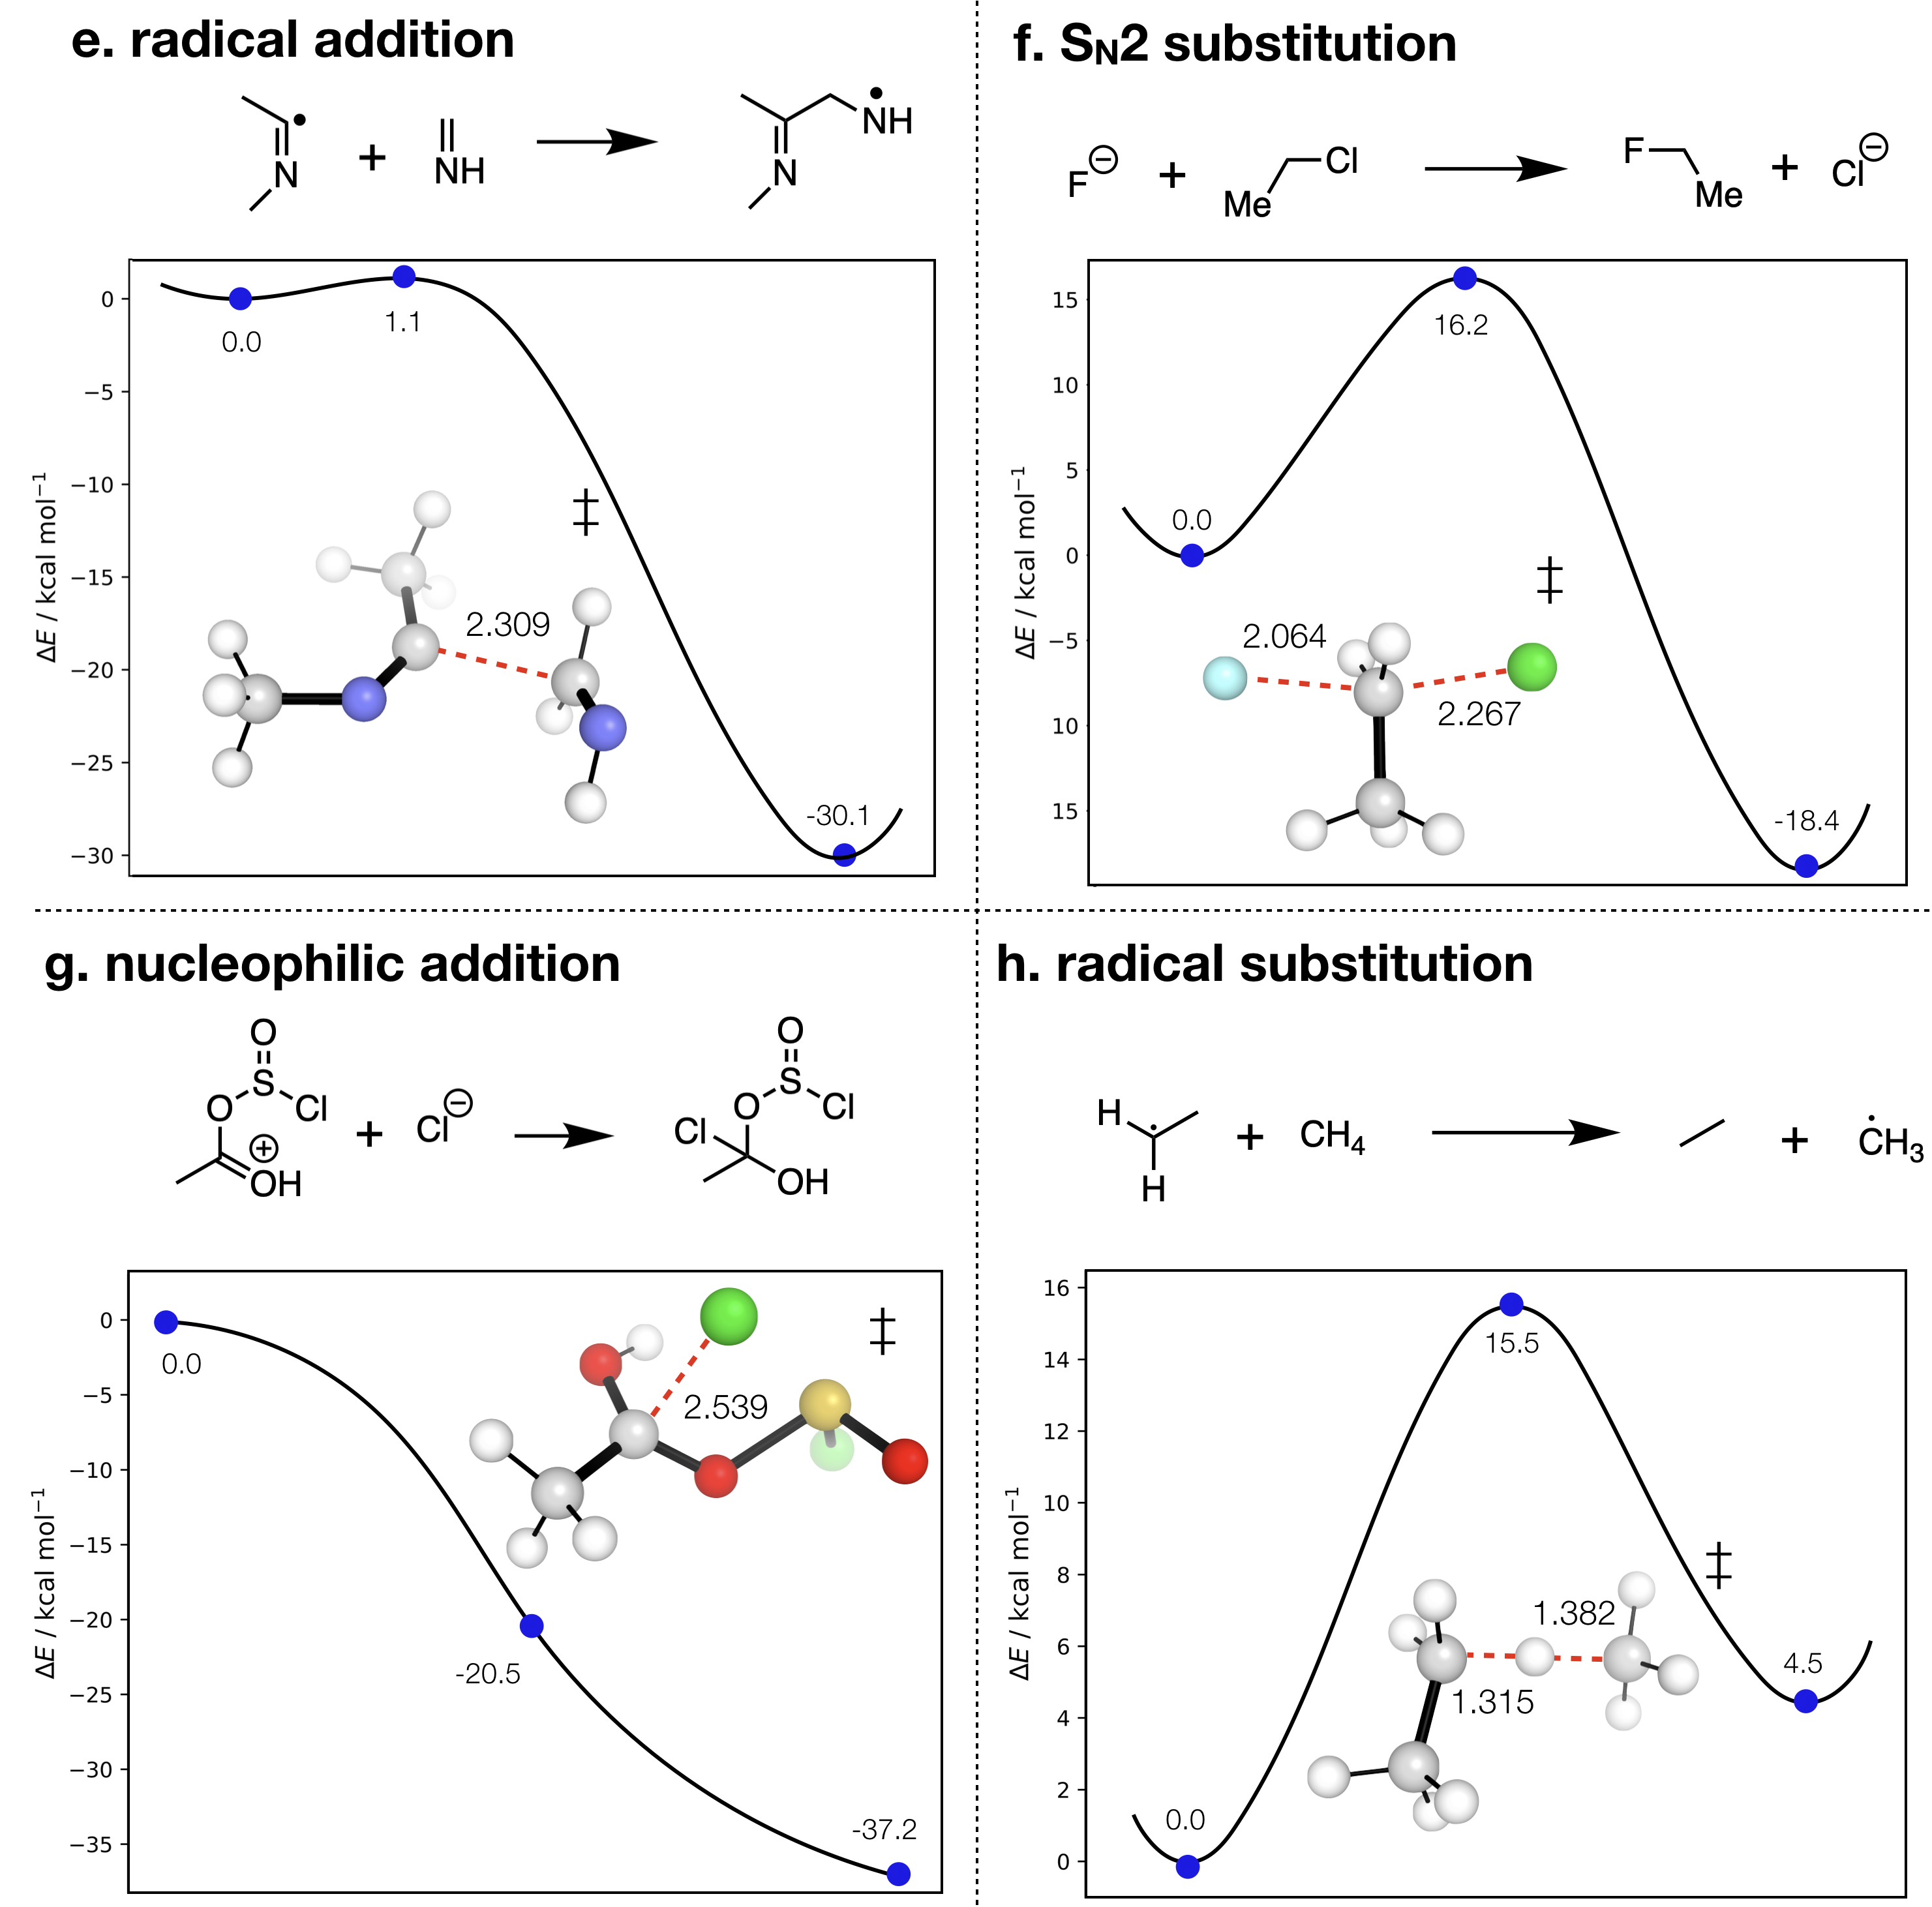
\includegraphics[width=\textwidth]{5/autode/figs/figS18e-h}
	\vspace{0.2cm}
	\hrule
	\caption{\figurename{ \ref{fig::ade_si_18a}} continued.}
	\label{fig::ade_si_18e}
\end{figure}


\begin{figure}[h!]
	\vspace{0.4cm}
	\centering
	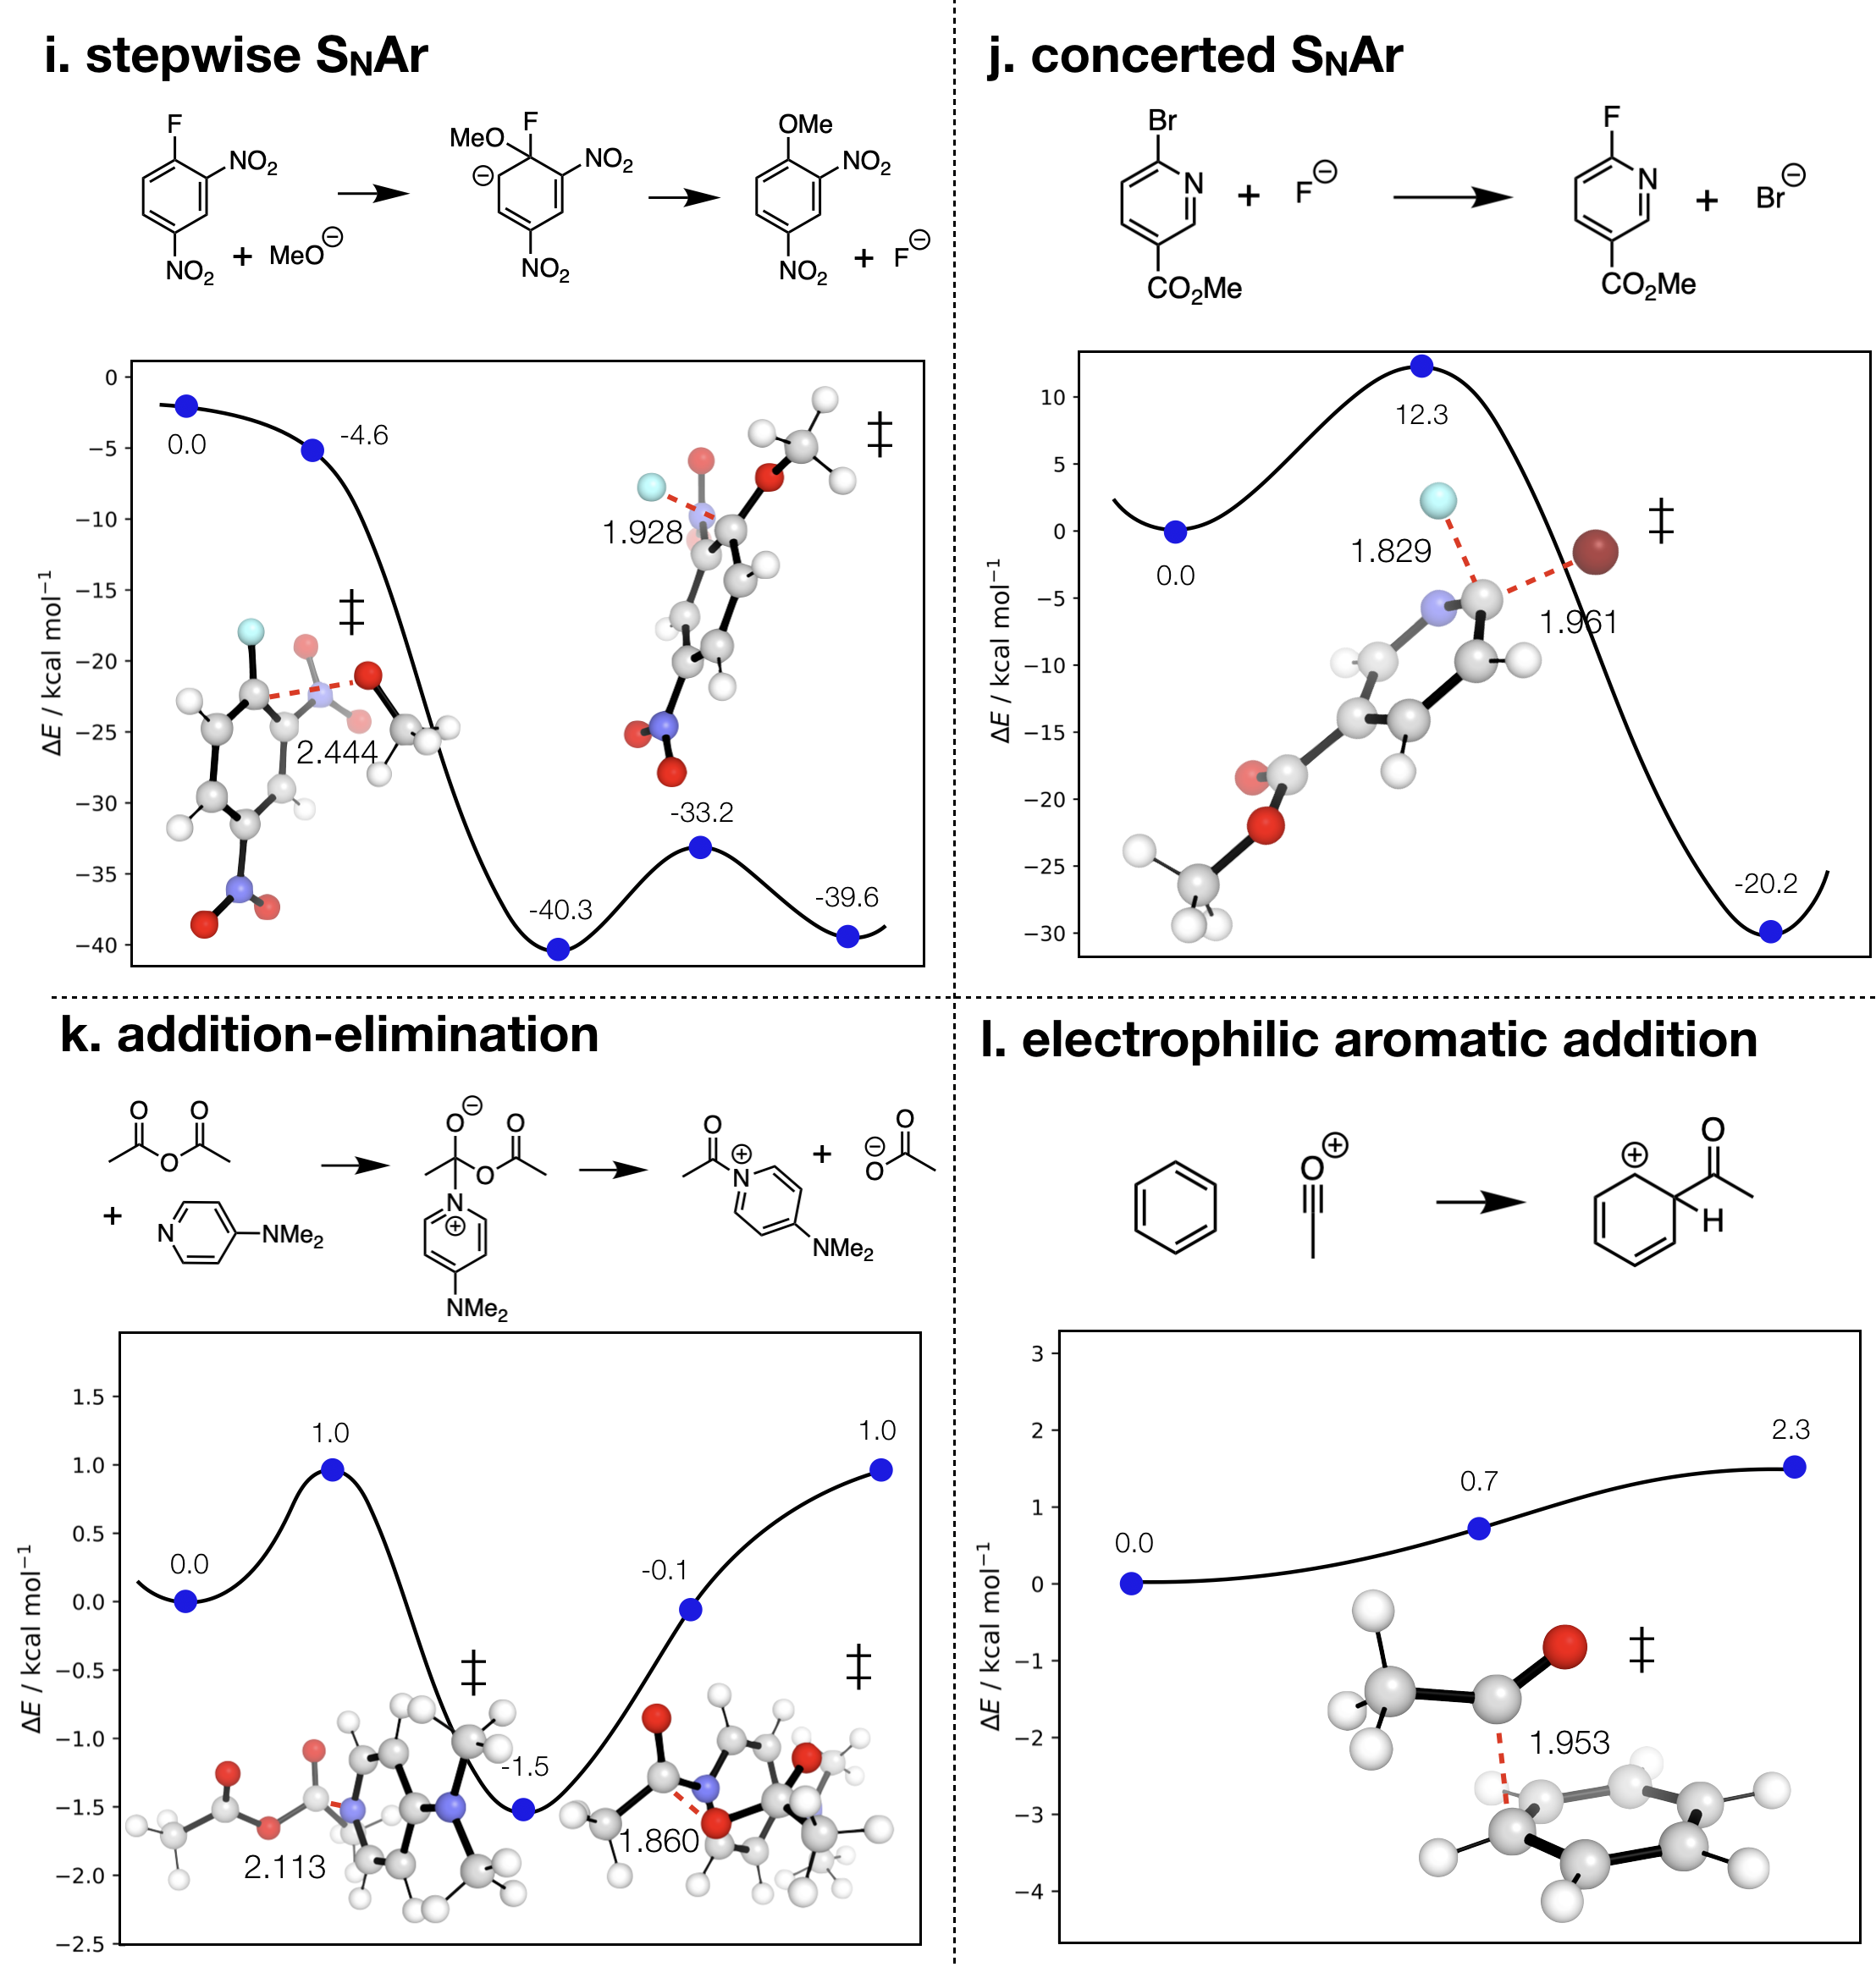
\includegraphics[width=\textwidth]{5/autode/figs/figS18i-l}
	\vspace{0.2cm}
	\hrule
	\caption{\figurename{ \ref{fig::ade_si_18a}} continued.}
	\label{fig::ade_si_18i}
\end{figure}


\begin{figure}[h!]
	\vspace{0.4cm}
	\centering
	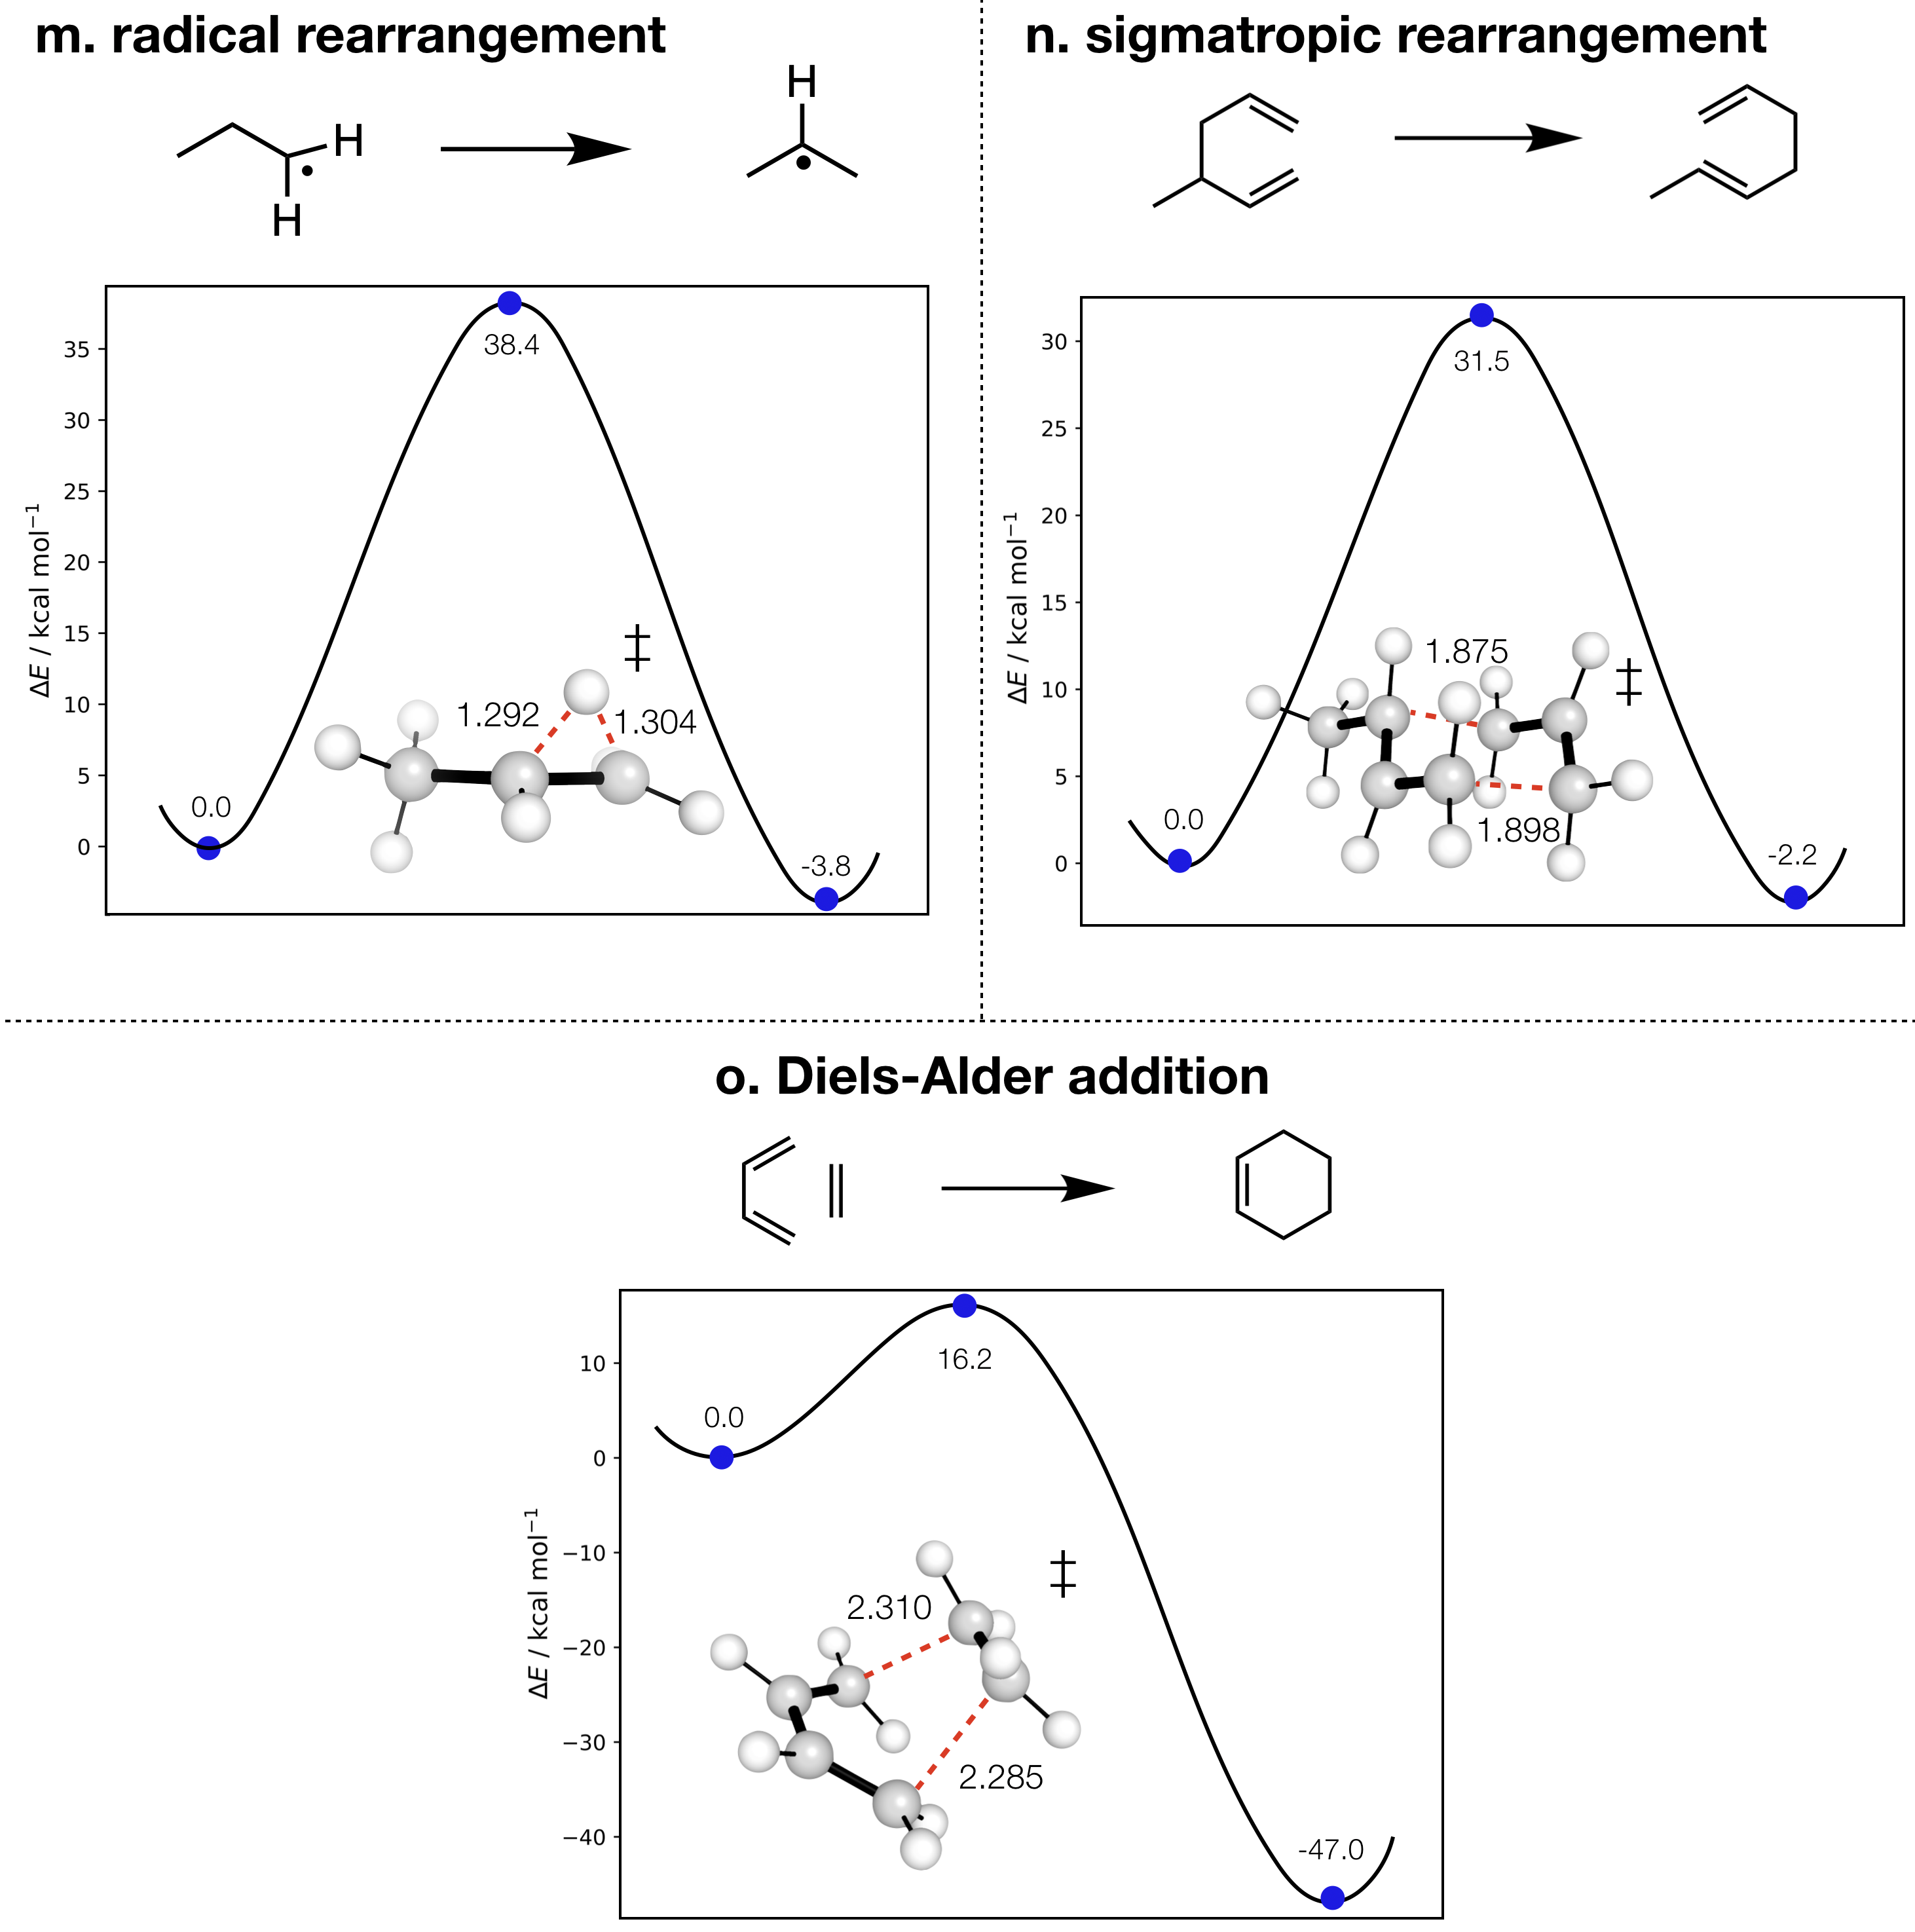
\includegraphics[width=\textwidth]{5/autode/figs/figS18m-o}
	\vspace{0.2cm}
	\hrule
	\caption{\figurename{ \ref{fig::ade_si_18a}} continued.}
	\label{fig::ade_si_18m}
\end{figure}





% --------------------------------------------------------------------------------------------
% ------------------------------------- Joe's examples --------------------------------------
% --------------------------------------------------------------------------------------------
\iffalse
\begin{figure}[h!]
	\vspace{0.4cm}
	\centering
	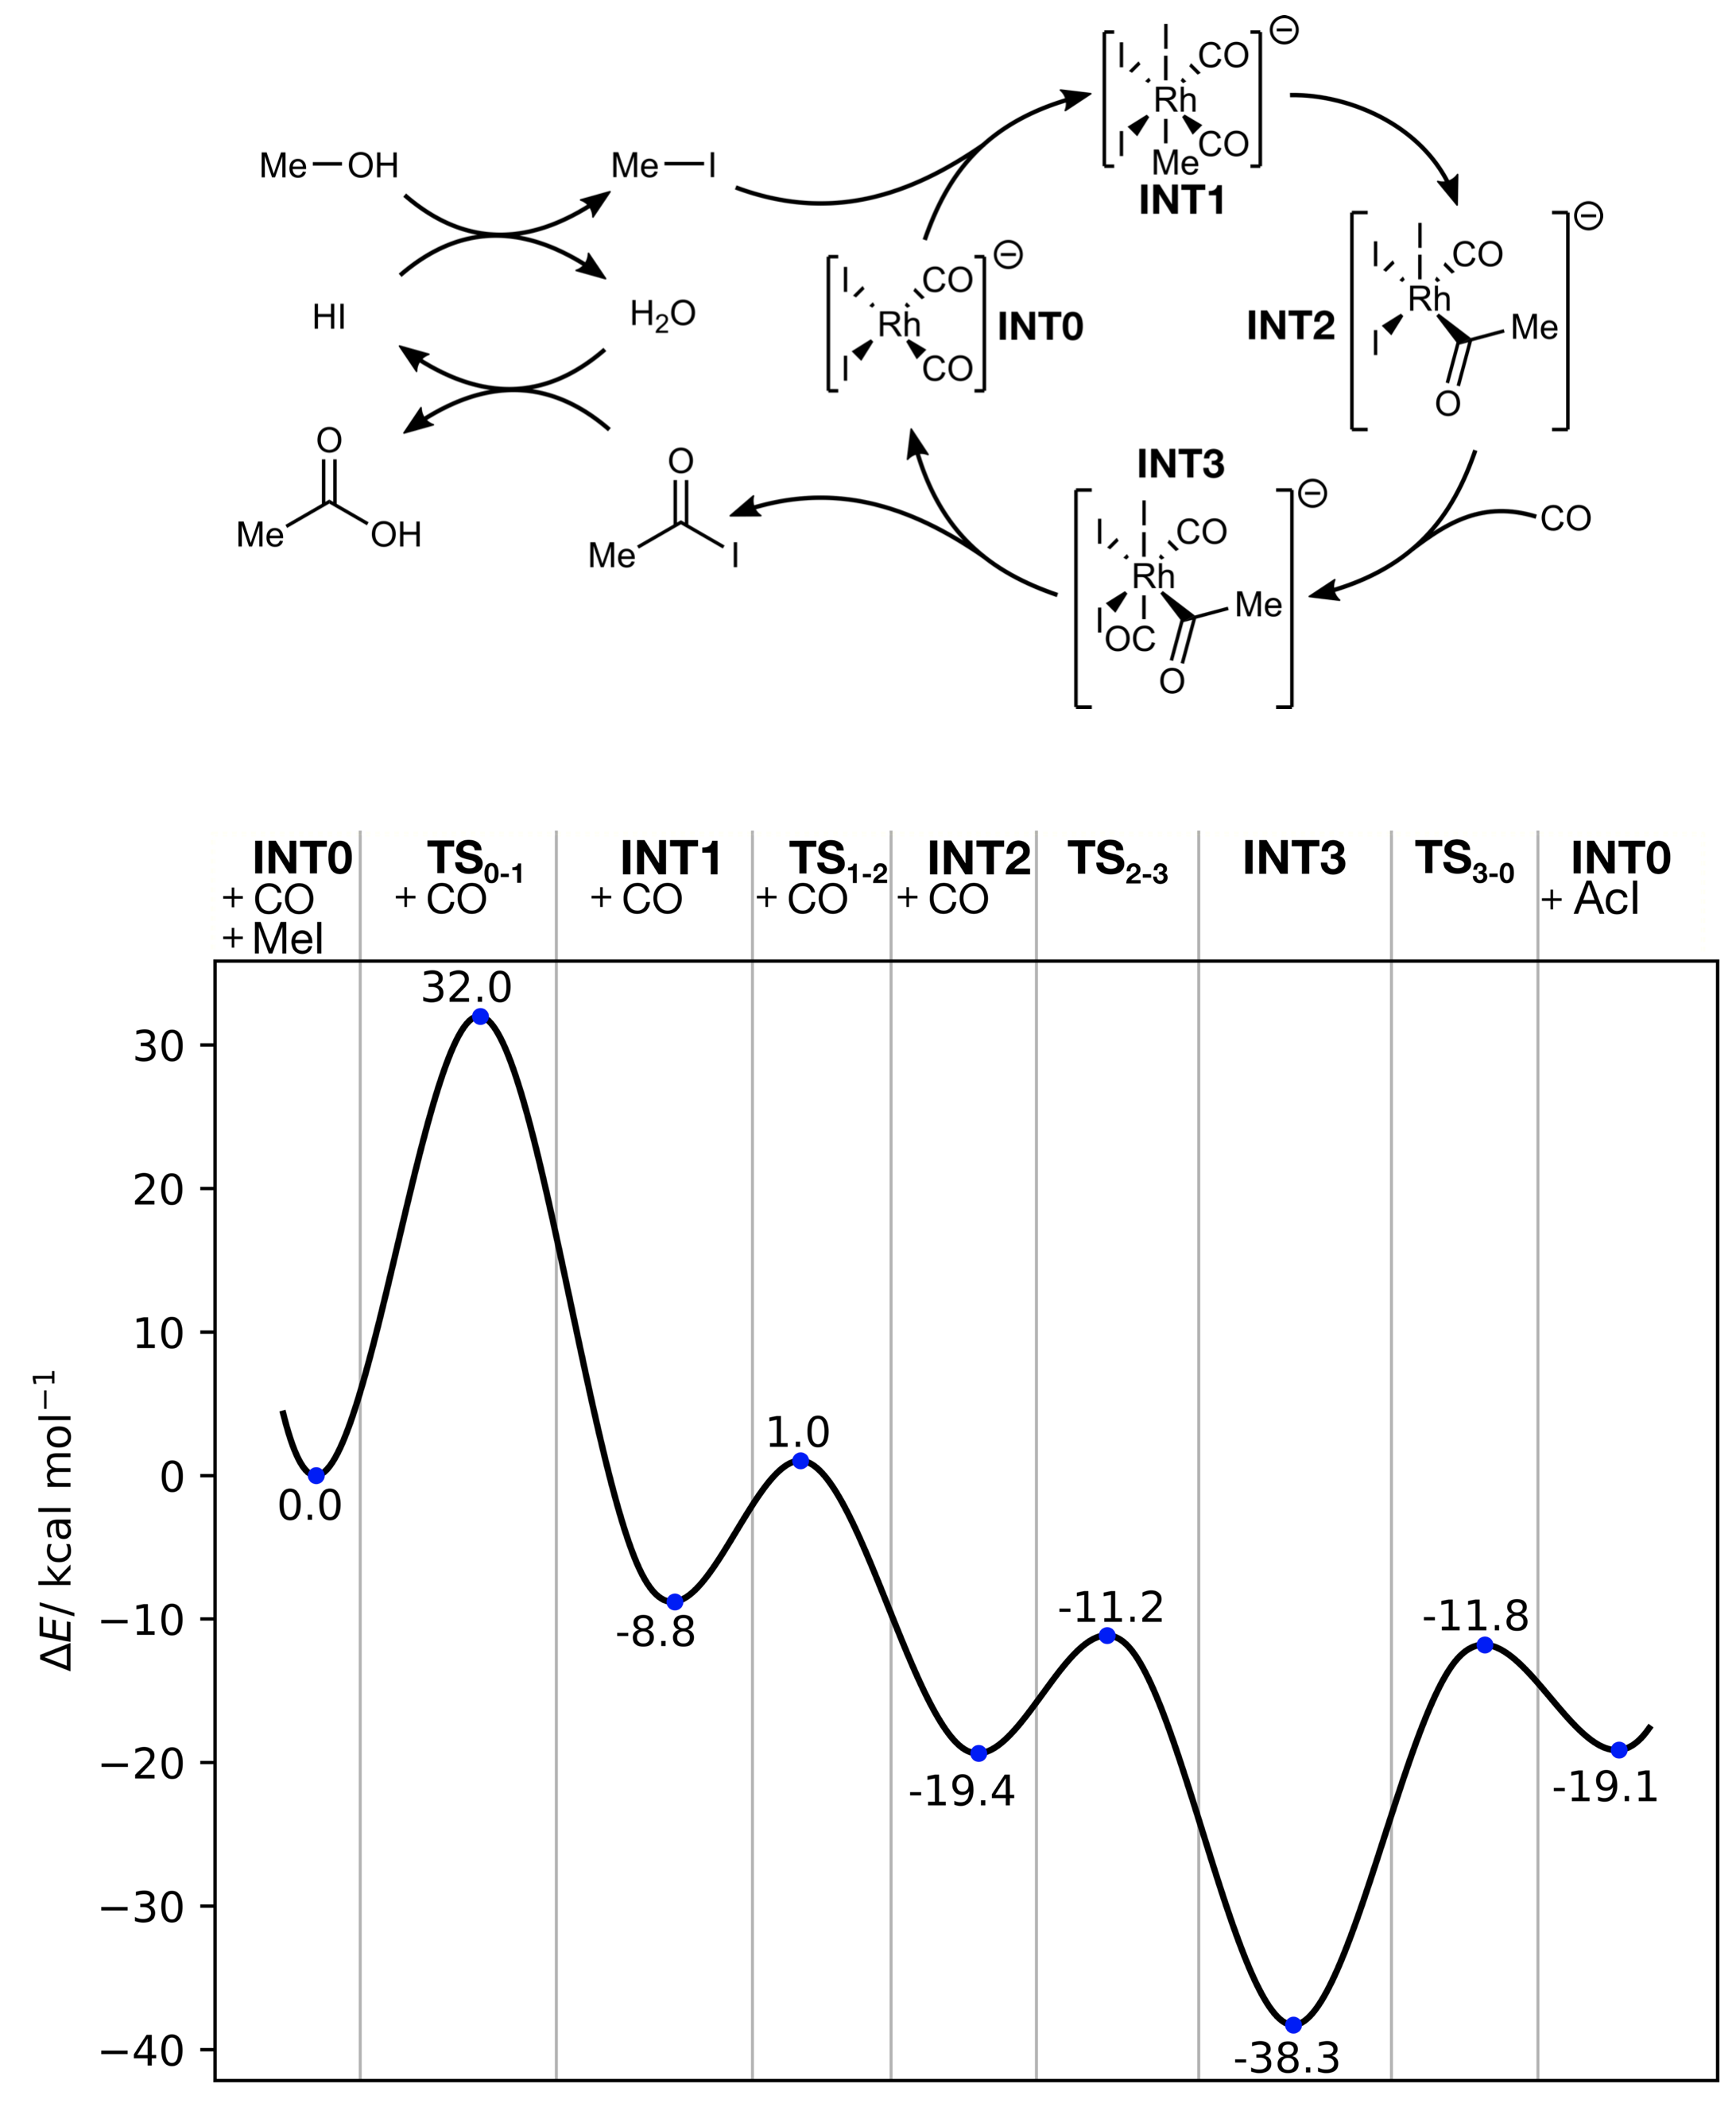
\includegraphics[width=14cm]{5/autode/figs/figS19}
	\vspace{0.2cm}
	\hrule
	\caption{Rh-catalysed methanol carbonylation (Monsanto process) reaction profile generated in \ade (ORCA/XTB, PBE0-D3BJ/def2-TZVP//PBE0-D3BJ/def2-SVP).}
	\label{fig::ade_si_19}
\end{figure}

\begin{figure}[h!]
	\vspace{0.4cm}
	\centering
	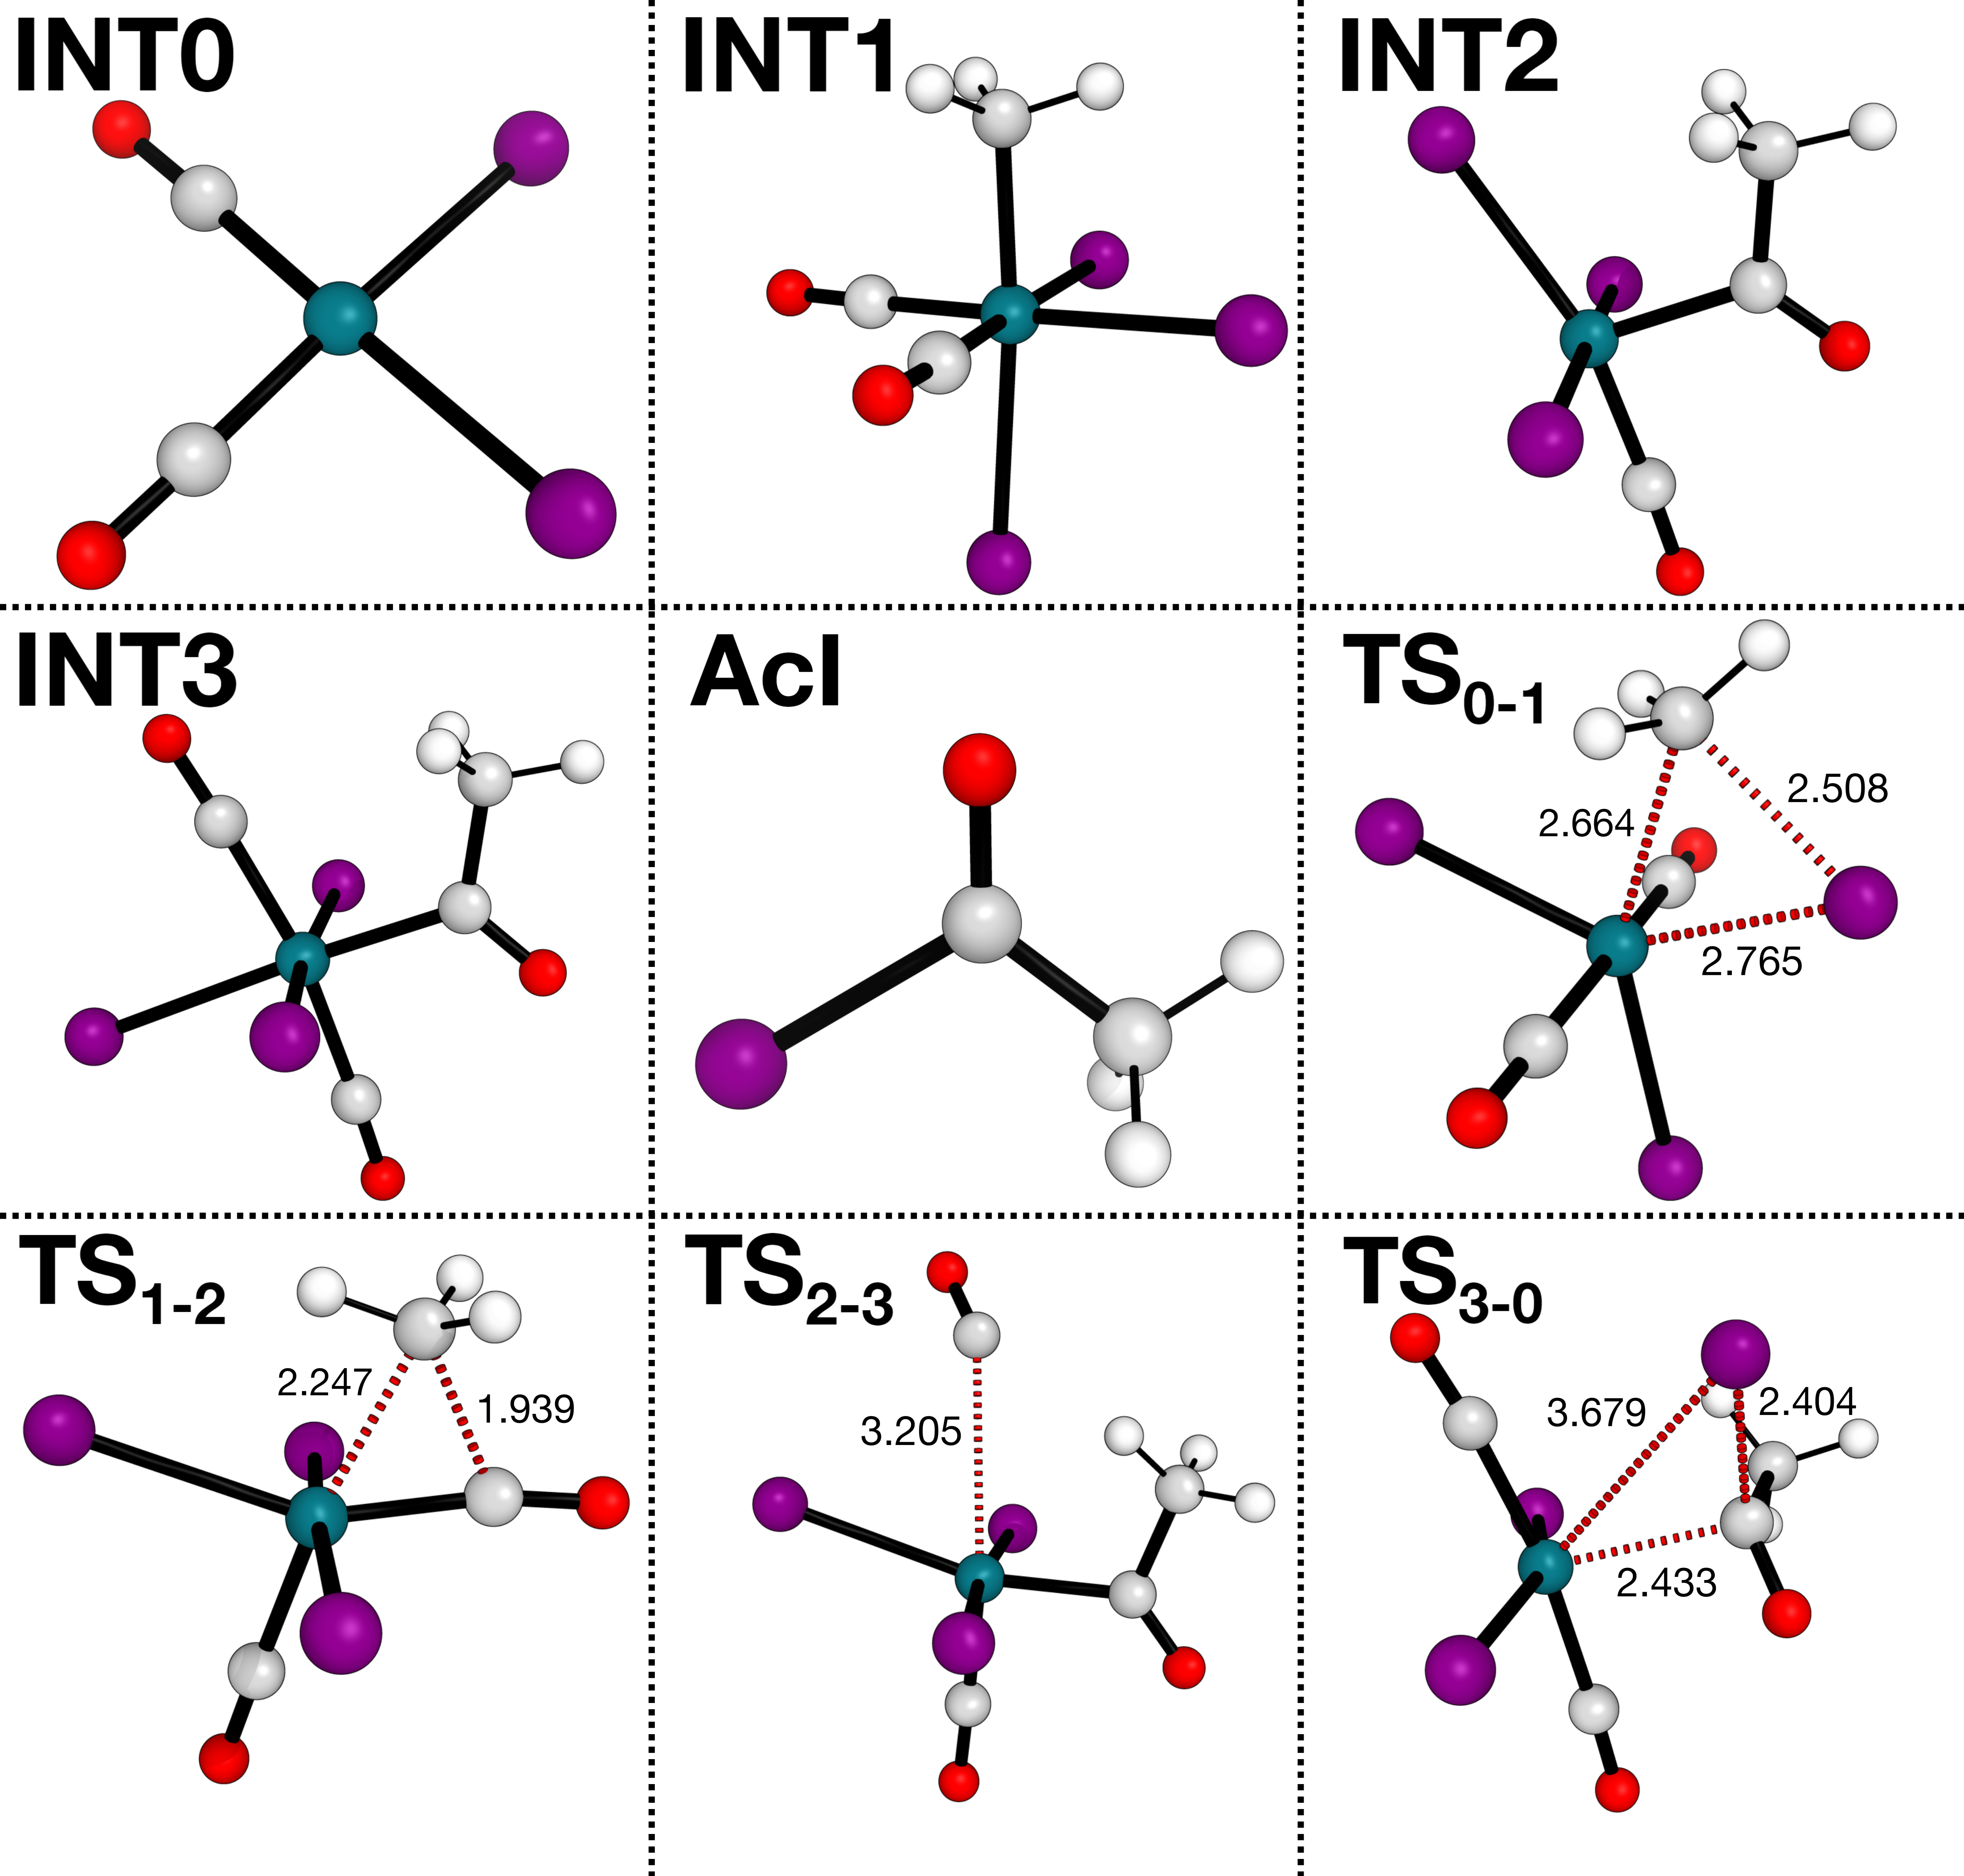
\includegraphics[width=13cm]{5/autode/figs/figS20}
	\vspace{0.2cm}
	\hrule
	\caption{Most stable intermediates and transition states for the reaction profile plotted in Figure \ref{fig::ade_si_19} located by \ade at the PBE-D3BJ/def2-SVP level of theory.}
	\label{fig::ade_si_20}
\end{figure}

\begin{figure}[h!]
\vspace{0.4cm}
\centering
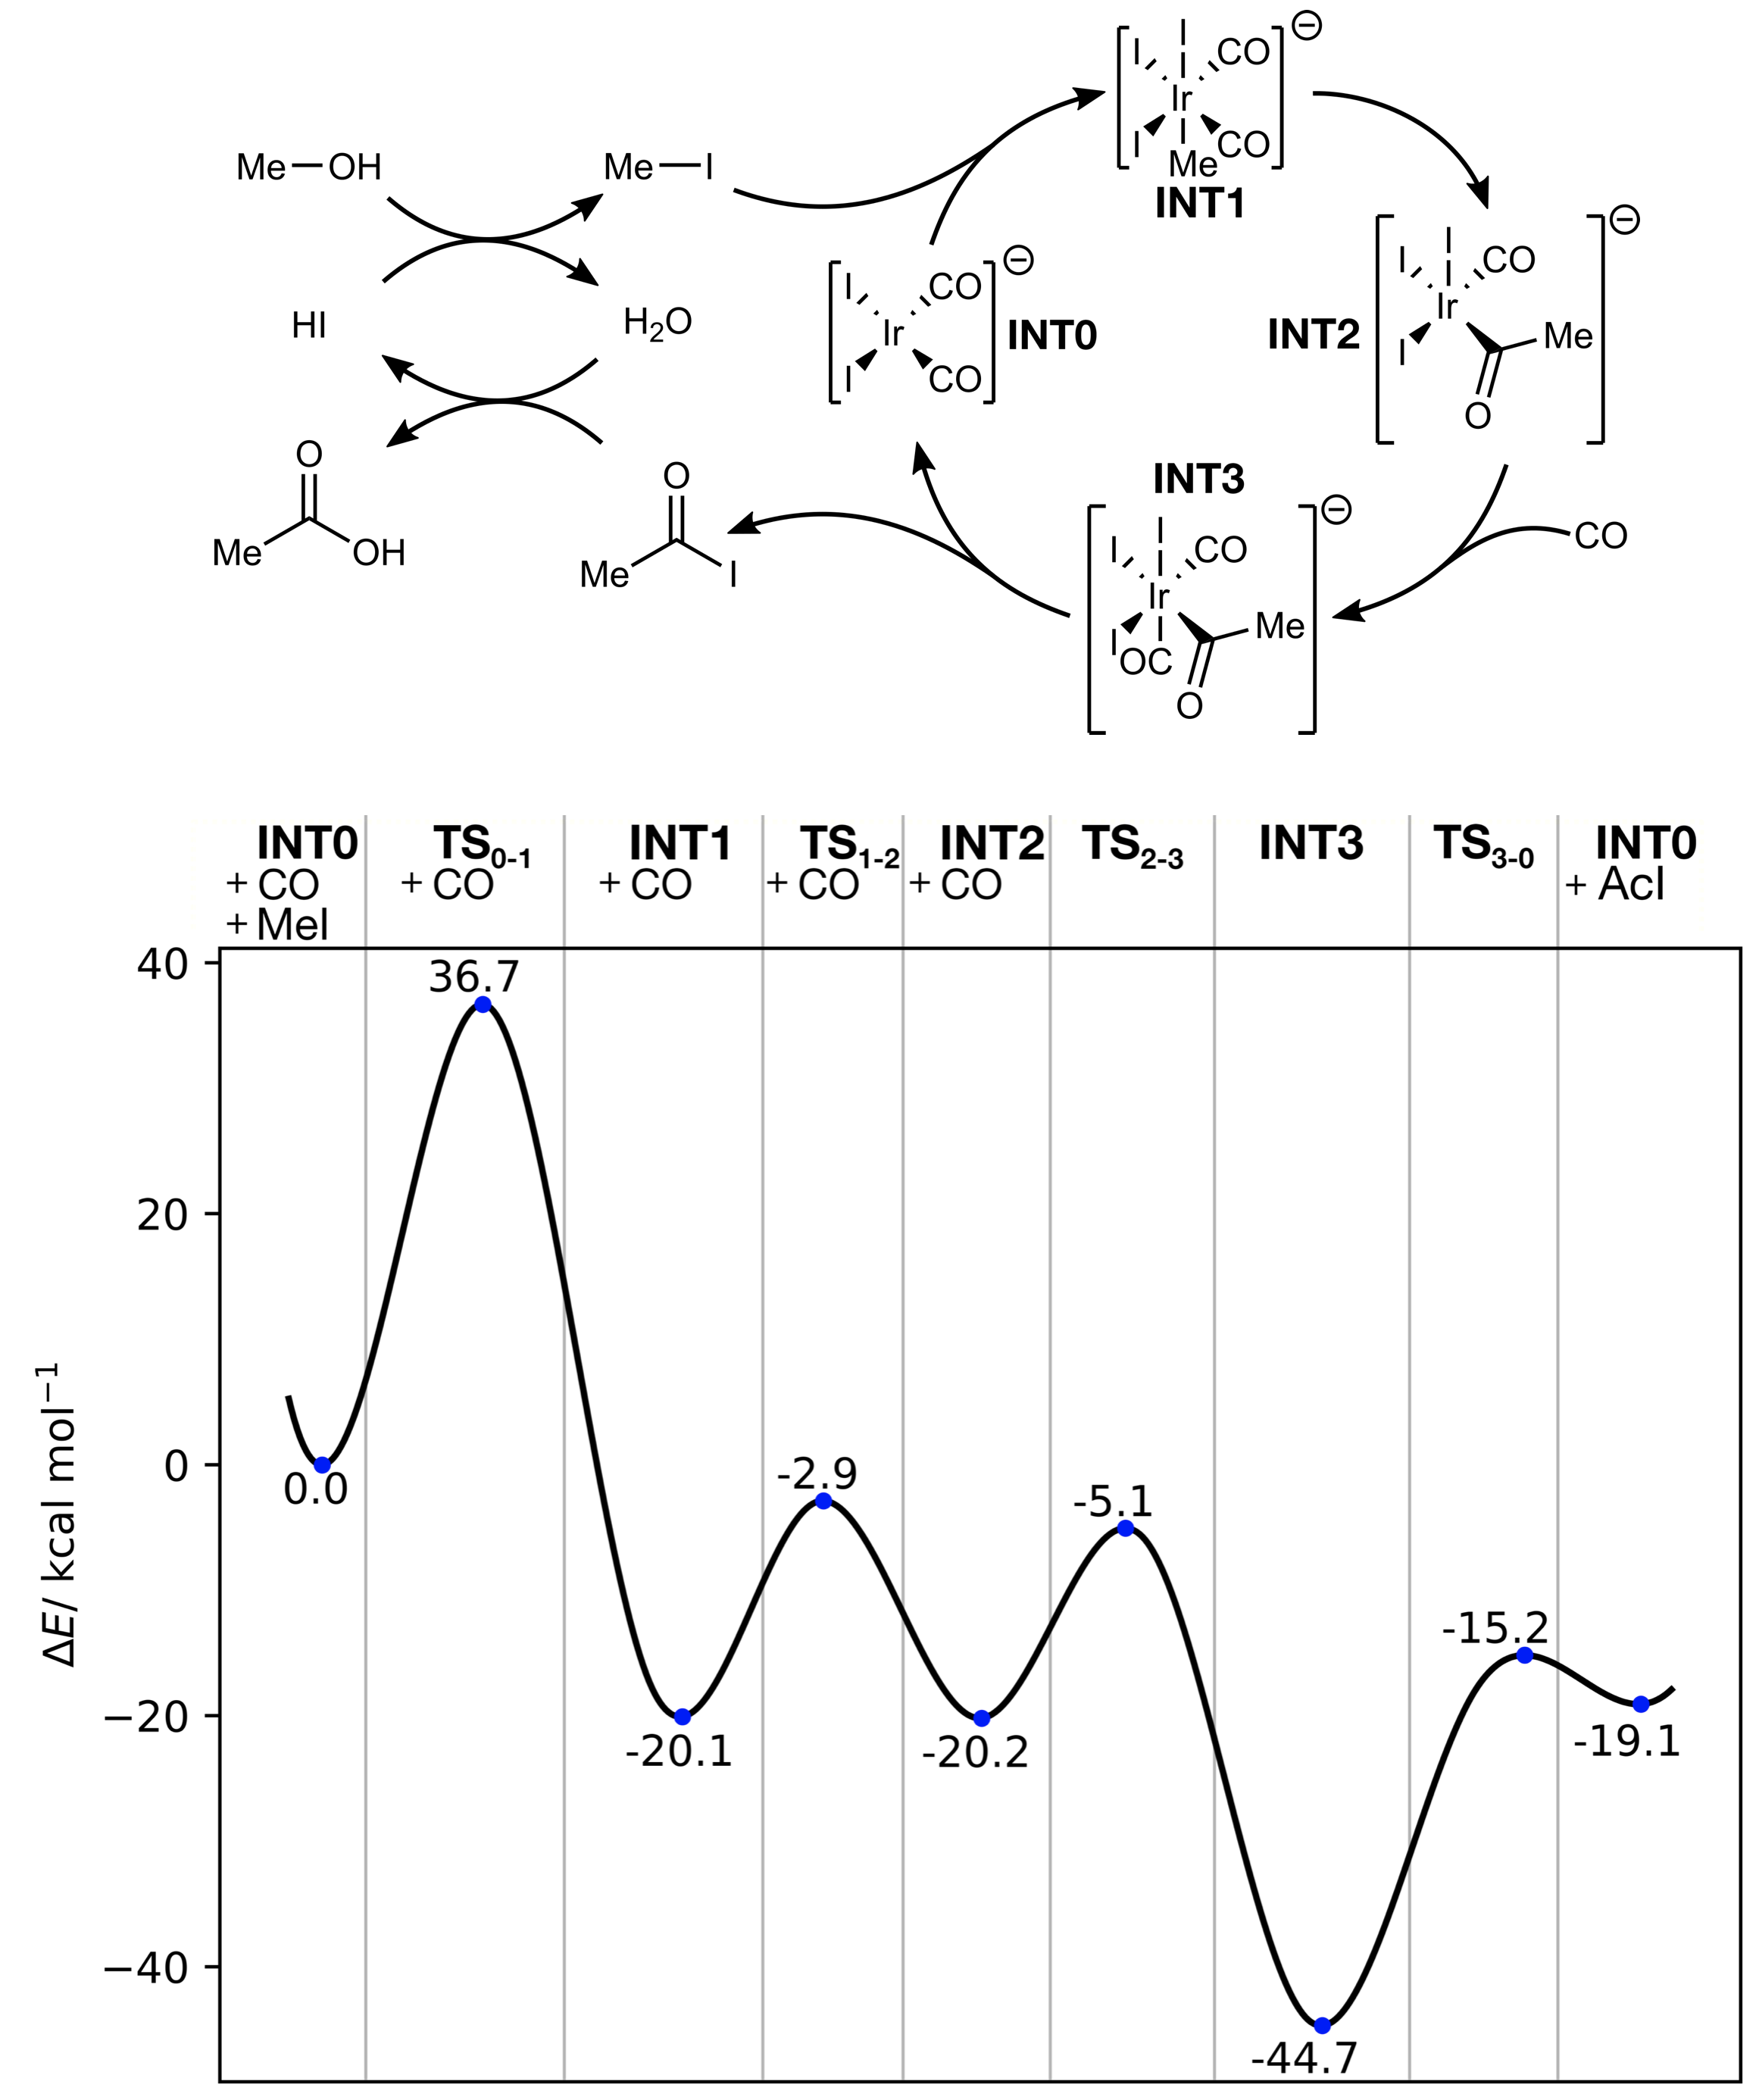
\includegraphics[width=14cm]{5/autode/figs/figS21}
\vspace{0.2cm}
\hrule
\caption{Ir-catalysed methanol carbonylation (Cativa process) reaction profile generated in \ade (ORCA/XTB, PBE0-D3BJ/def2-TZVP//PBE0-D3BJ/def2-SVP).}
\label{fig::ade_si_21}
\end{figure}

\begin{figure}[h!]
	\vspace{0.4cm}
	\centering
	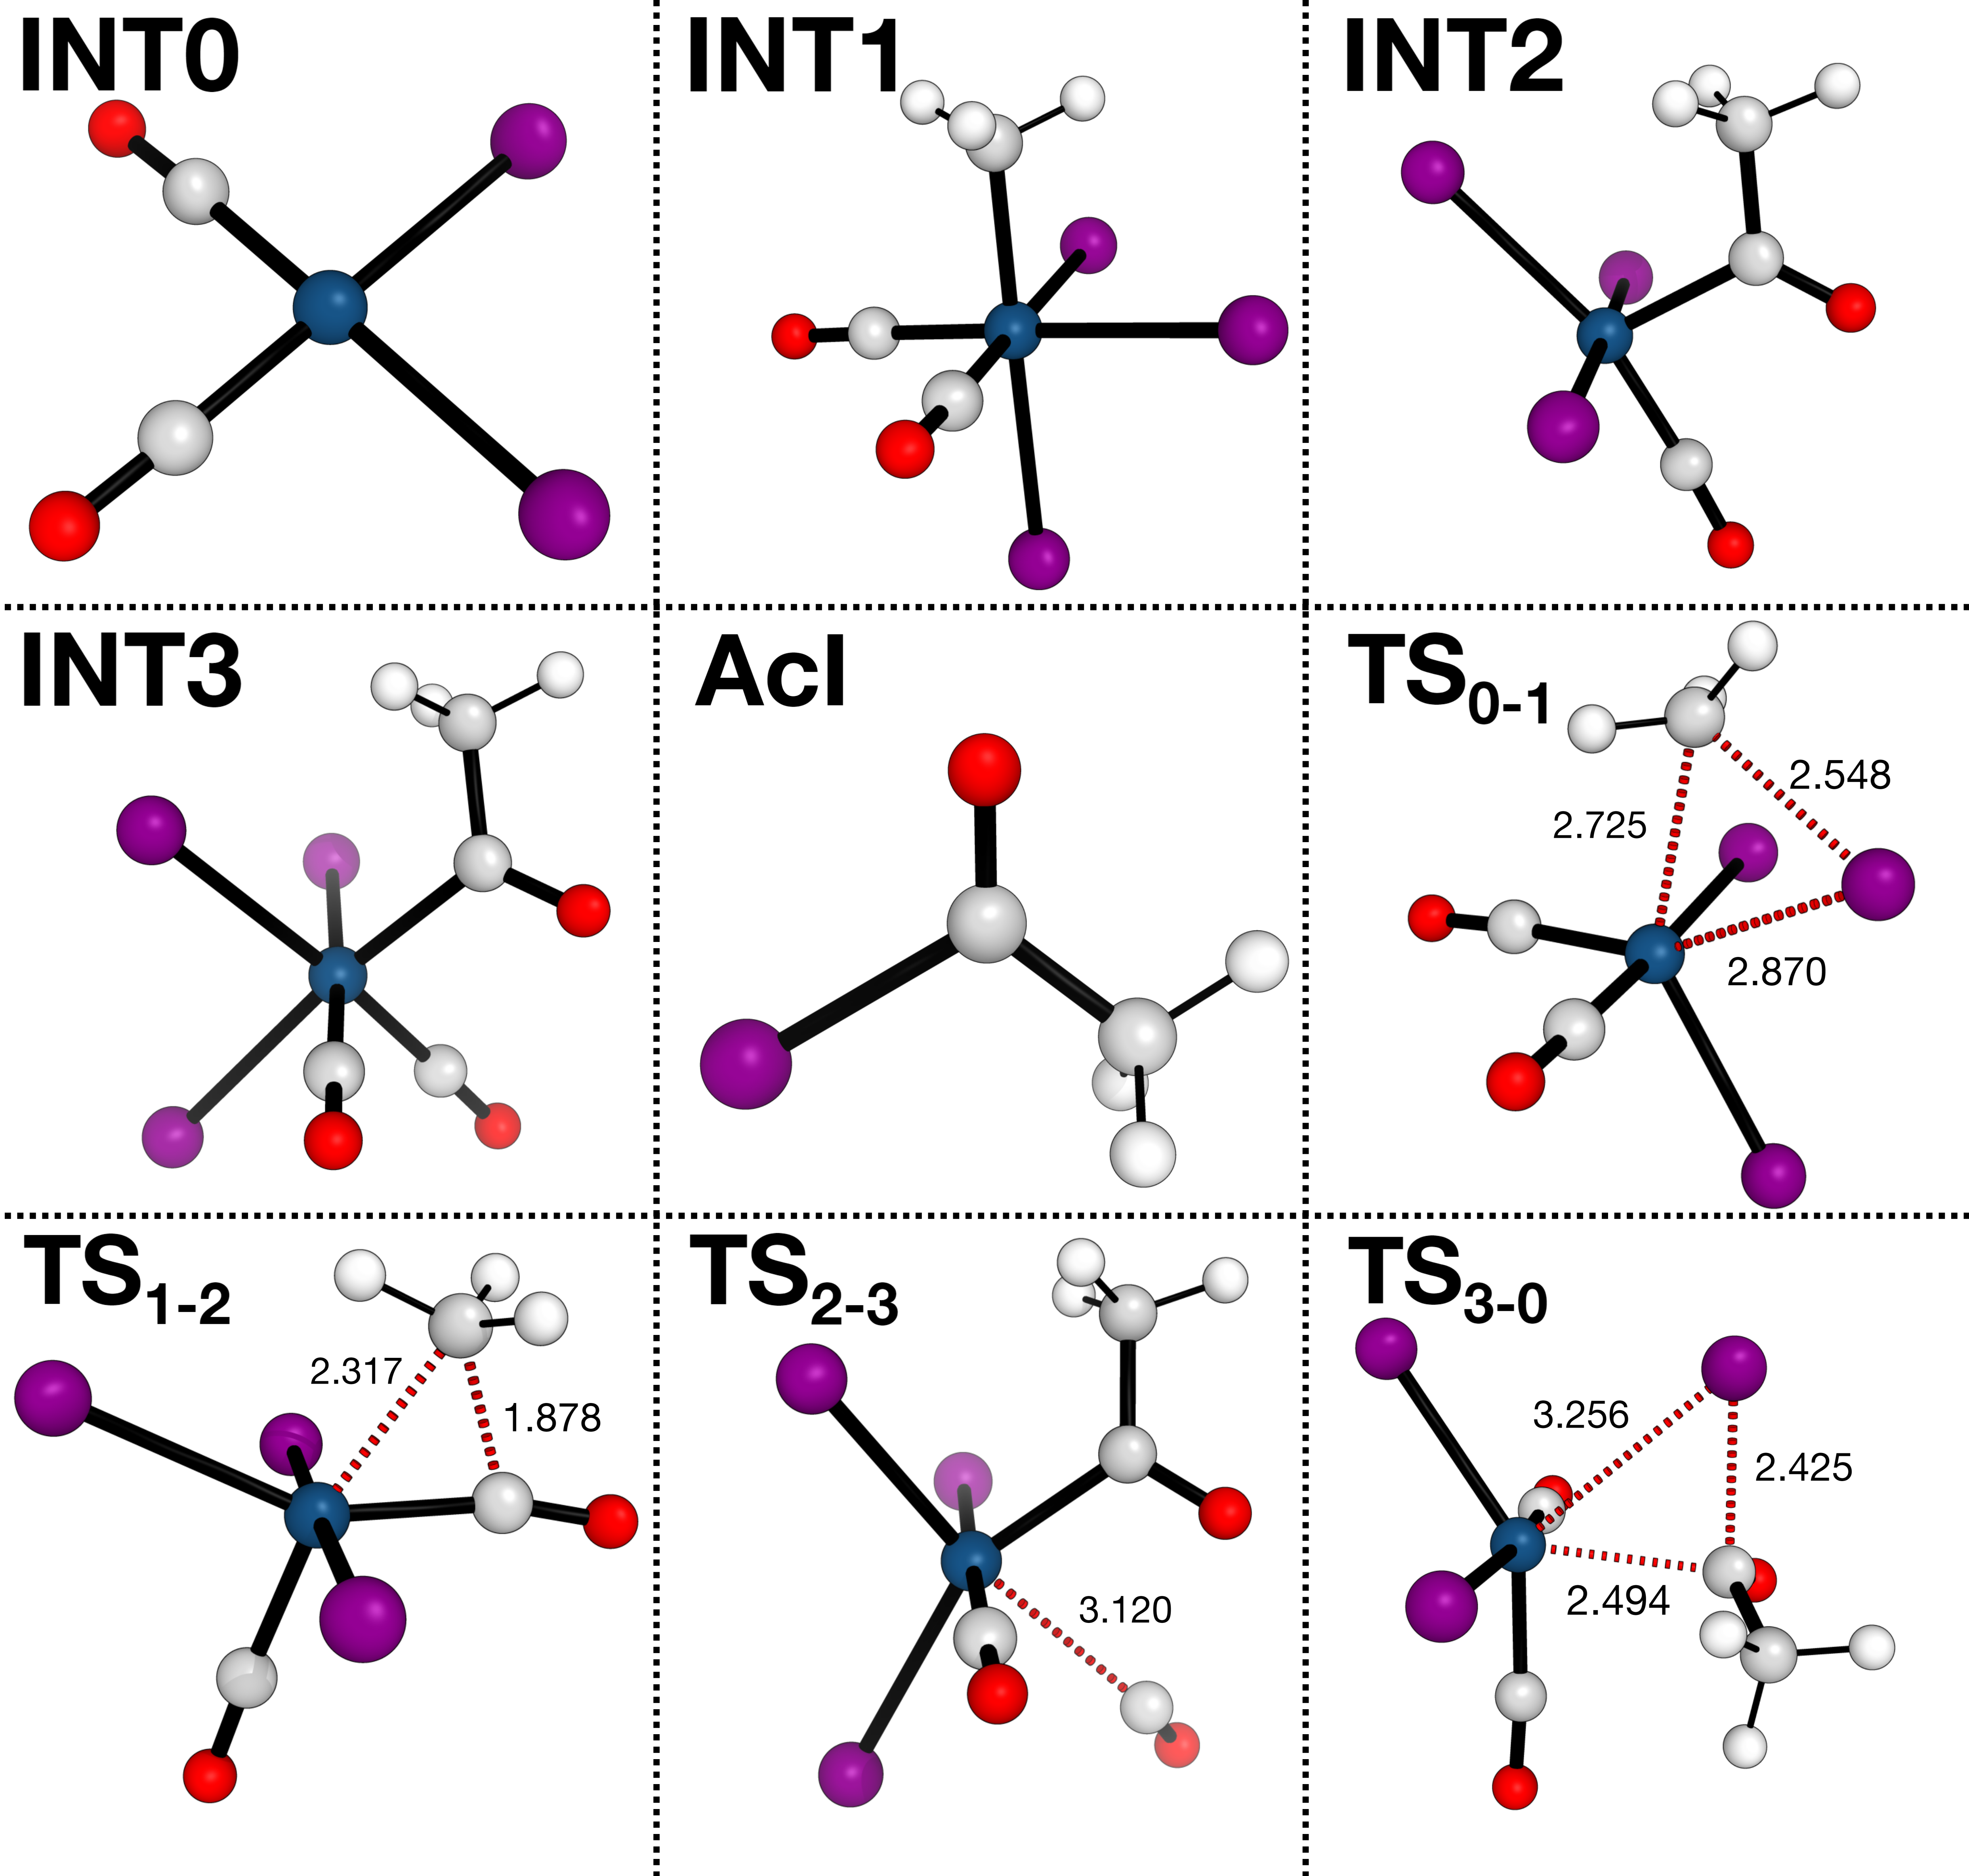
\includegraphics[width=13cm]{5/autode/figs/figS22}
	\vspace{0.2cm}
	\hrule
	\caption{Most stable intermediates and transition states for the reaction profile shown in Figure \ref{fig::ade_si_20} located by \ade at the PBE-D3BJ/def2-SVP level of theory. Distances quoted in \AA.}
	\label{fig::ade_si_22}
\end{figure}
\fi
% --------------------------------------------------------------------------------------------



\begin{figure}[h!]
	\vspace{0.4cm}
	\centering
	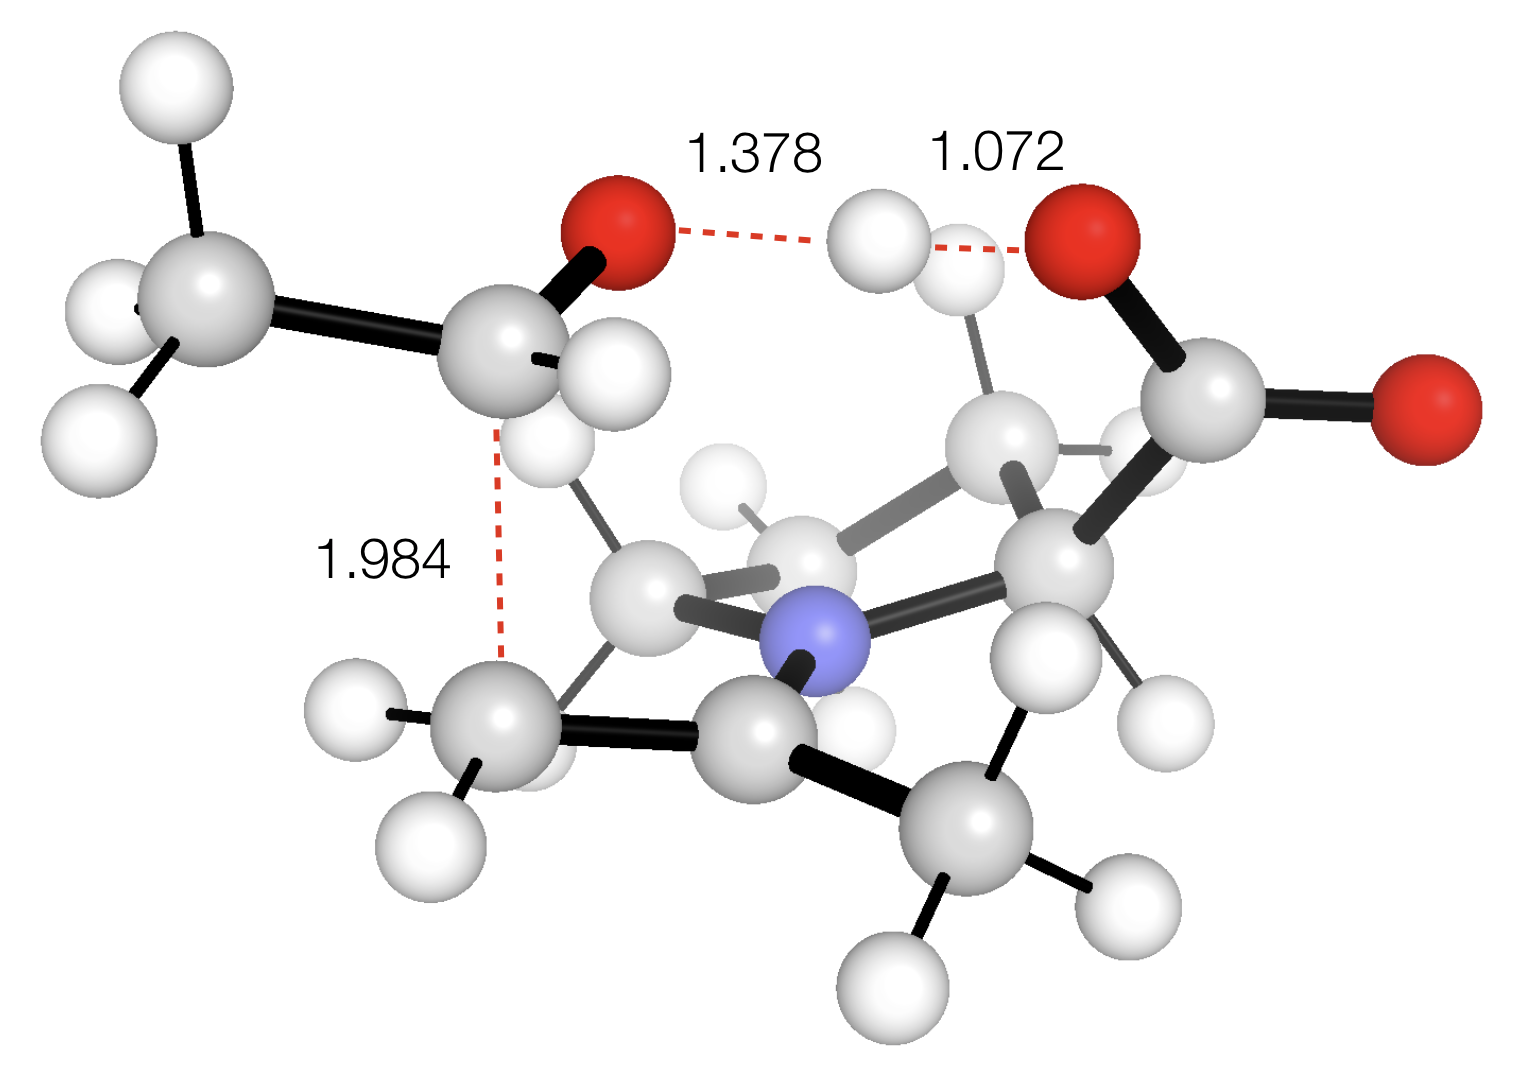
\includegraphics[width=7cm]{5/autode/figs/figS23}
	\vspace{0.2cm}
	\hrule
	\caption{Houk-List TS for an asymmetric aldol reaction found with \ade (ORCA/XTB, PBE0-D3BJ/def2-TZVP//PBE0-D3BJ/def2-SVP). See full supporting information for input. Distances quoted in \AA.}
	\label{fig::ade_si_23}
\end{figure}

% --------------------------------------------------------------------------------------------
% ------------------------------------- More Joe examples ----------------------------------
% --------------------------------------------------------------------------------------------
\iffalse

\clearpage
\subsection{Further Examples}

57 reactions of carbenes into the C–H bonds of acetonitrile, isobutane and methane, reported in ref.\cite{Mieusset2008} showing the excellent correlation between manually obtained TSs and those found in an automated fashion with \ade.


\begin{figure}[h!]
	\vspace{0.4cm}
	\centering
	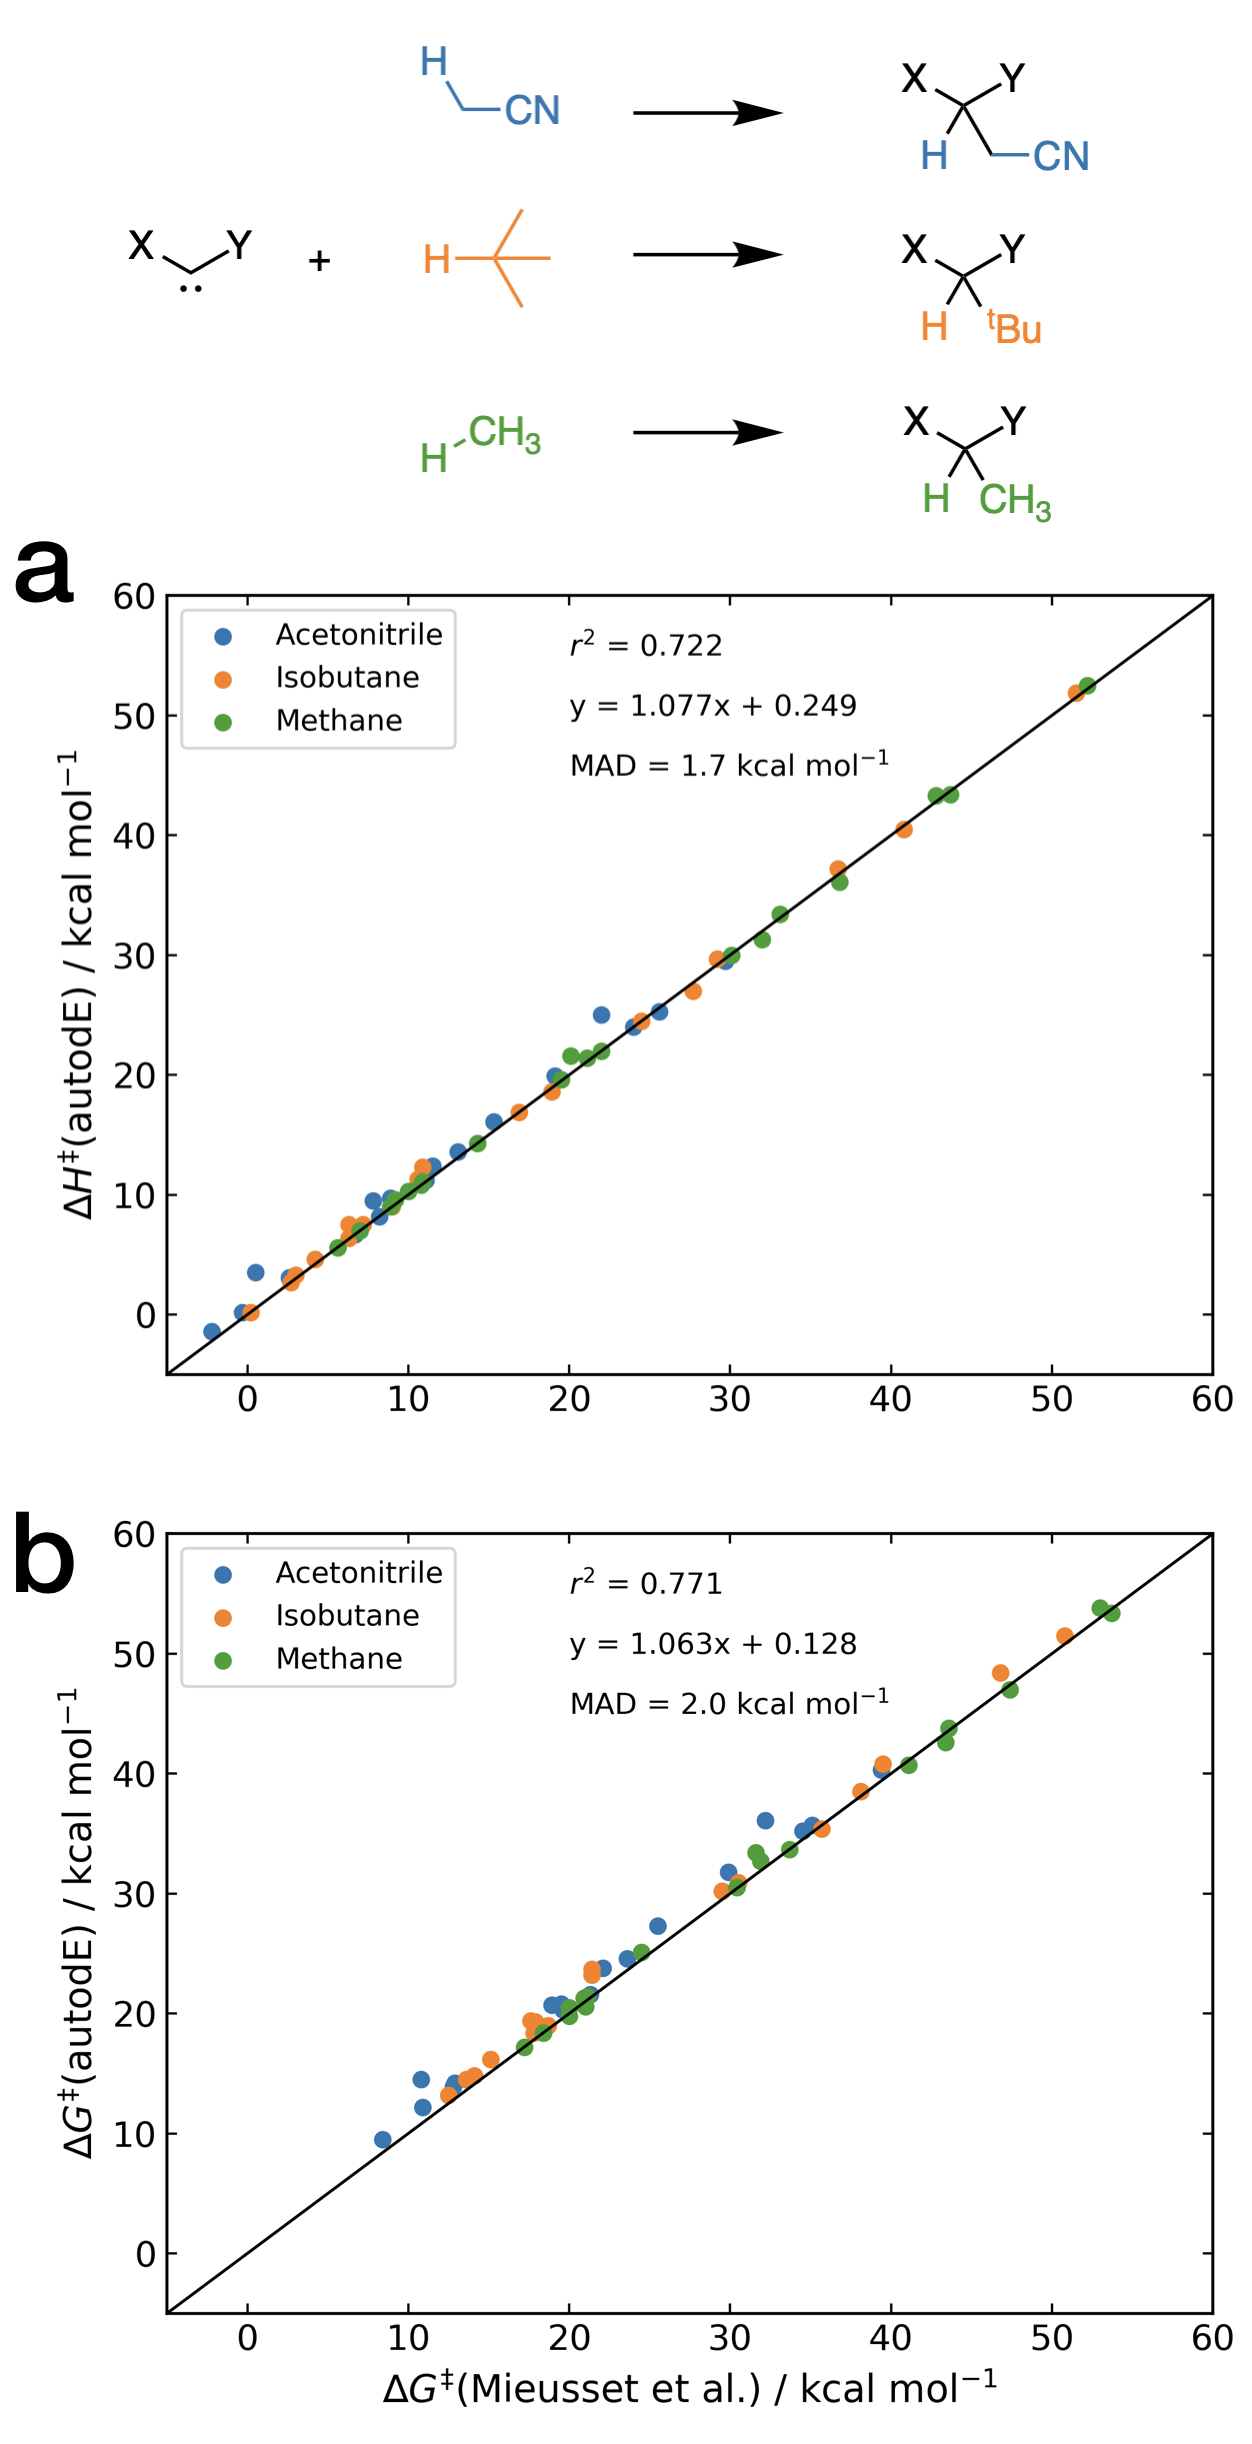
\includegraphics[width=9.5cm]{5/autode/figs/figS24}
	\vspace{0.2cm}
	\hrule
	\caption{Carbene-insertion barrier (a) enthalpies and (b) free energies. Calculations were performed at the same level of theory as the original work of Mieusset et. al in ref. \cite{Mieusset2008}. Values tabulated in the full supporting information.}
	\label{fig::ade_si_24}
\end{figure}


For Brevianamide formation \ade correctly identifies the relevant H-bond interaction (shown in black dashed lines) that leads to the formation of Brevianamide A, in agreement with previous computational studies by Domingo et al.\cite{Domingo1997}

\begin{figure}[h!]
	\vspace{0.4cm}
	\centering
	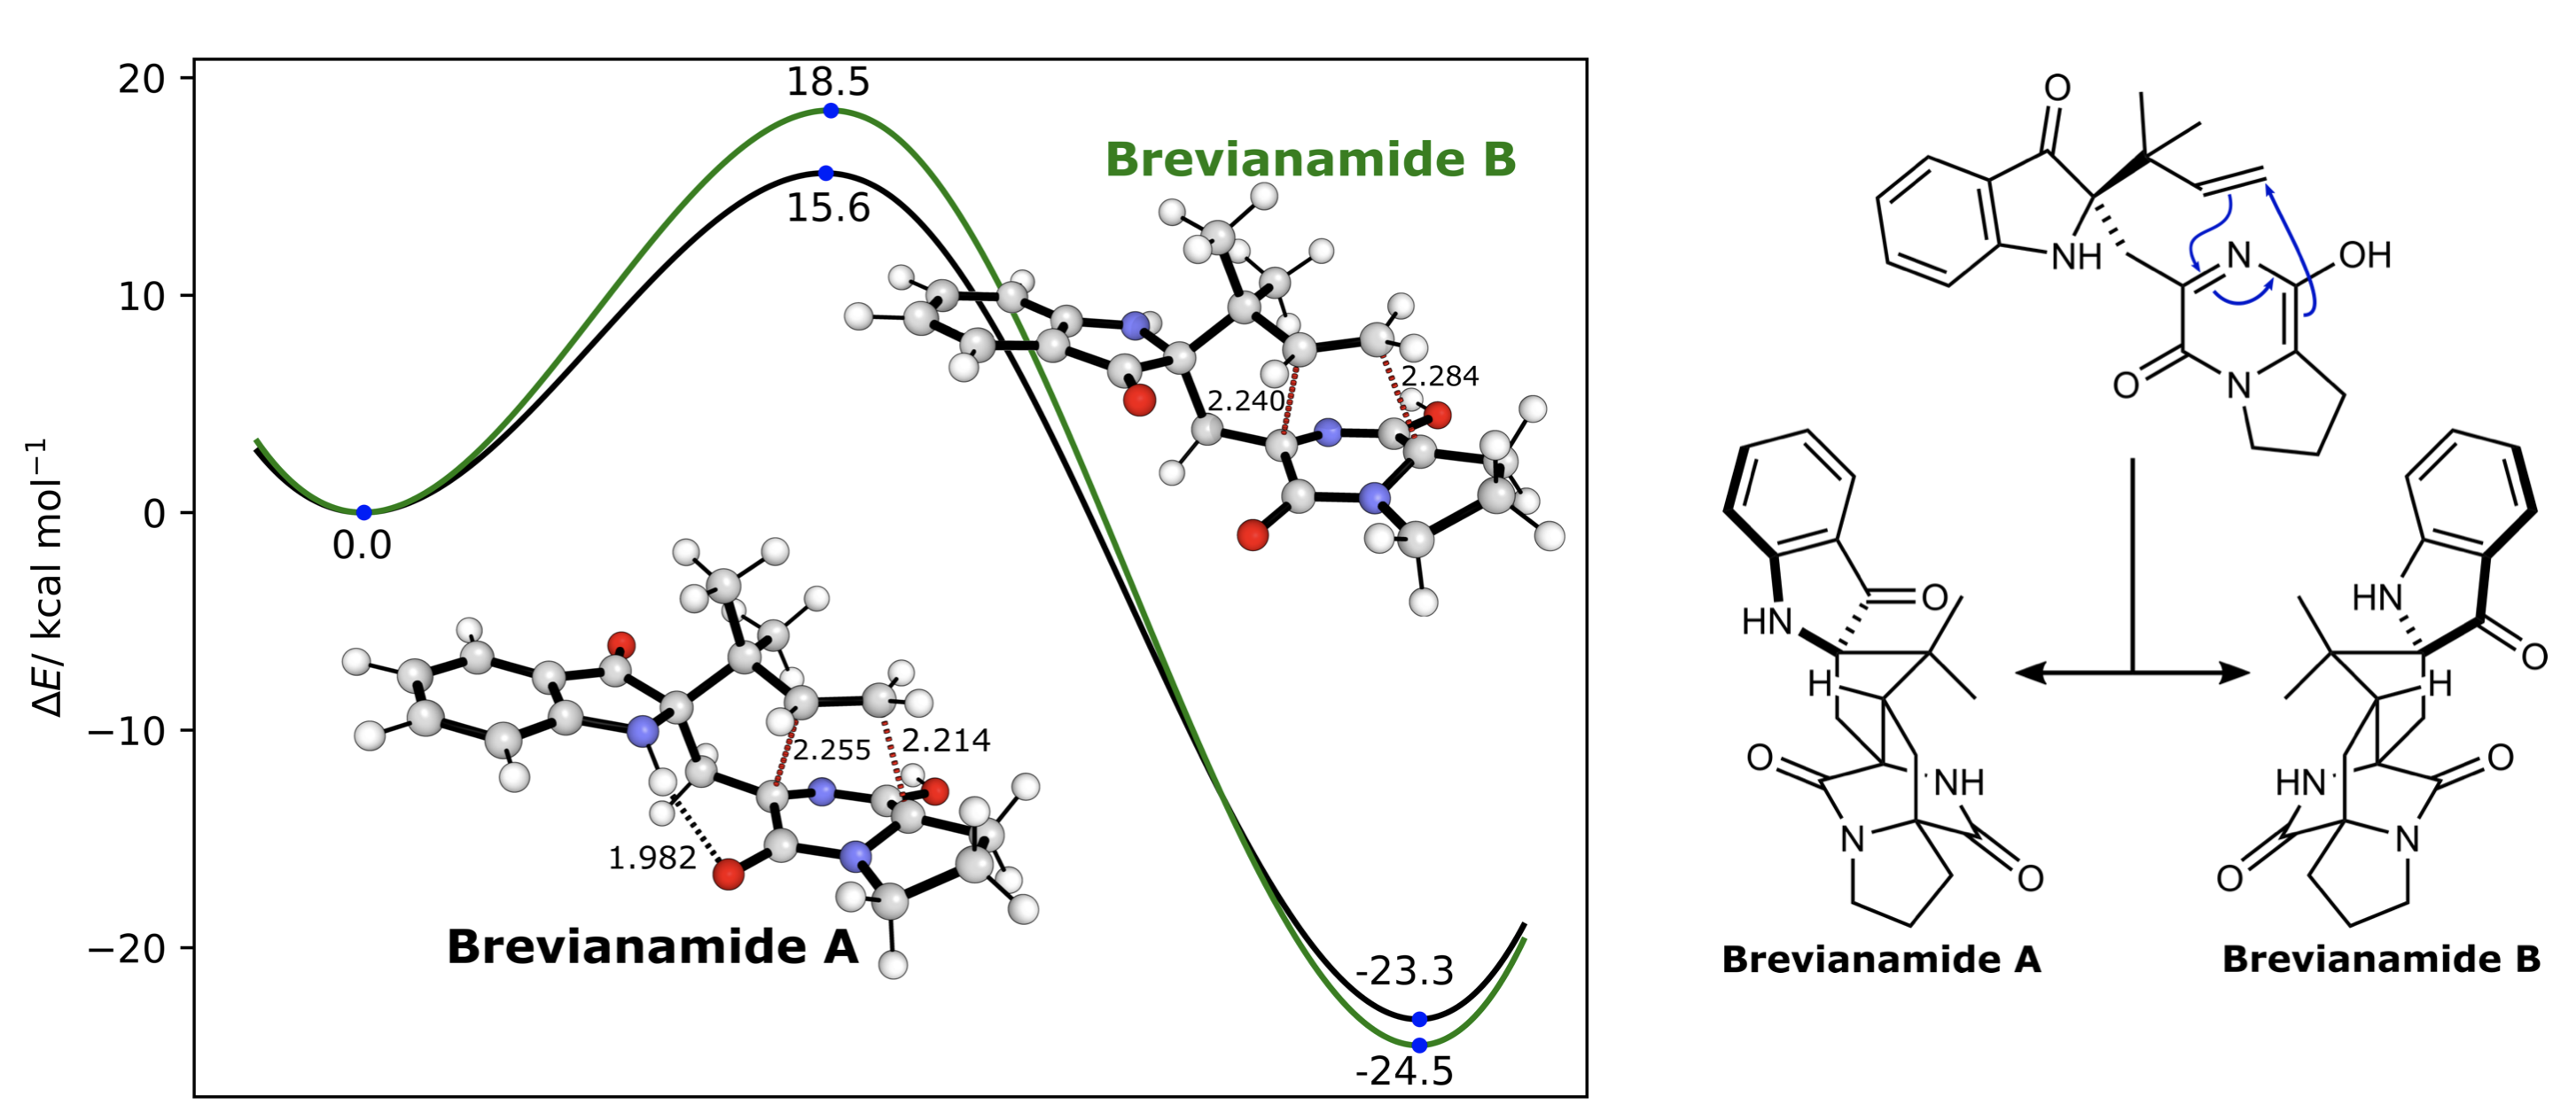
\includegraphics[width=\textwidth]{5/autode/figs/figS25}
	\vspace{0.2cm}
	\hrule
	\caption{Diels-alder reaction for the formation of Brevianamide A and B generated in \ade (ORCA/XTB, PBE0-D3BJ/def2-TZVP//PBE0-D3BJ/def2-SVP).}
	\label{fig::ade_si_25}
\end{figure}

In a diastereoselective epoxidation from ref.\cite{Schneebeli2009} \ade correctly locates this complex (2, 2) making breaking transition state in the preferred orientation.


\begin{figure}[h!]
	\vspace{0.4cm}
	\centering
	 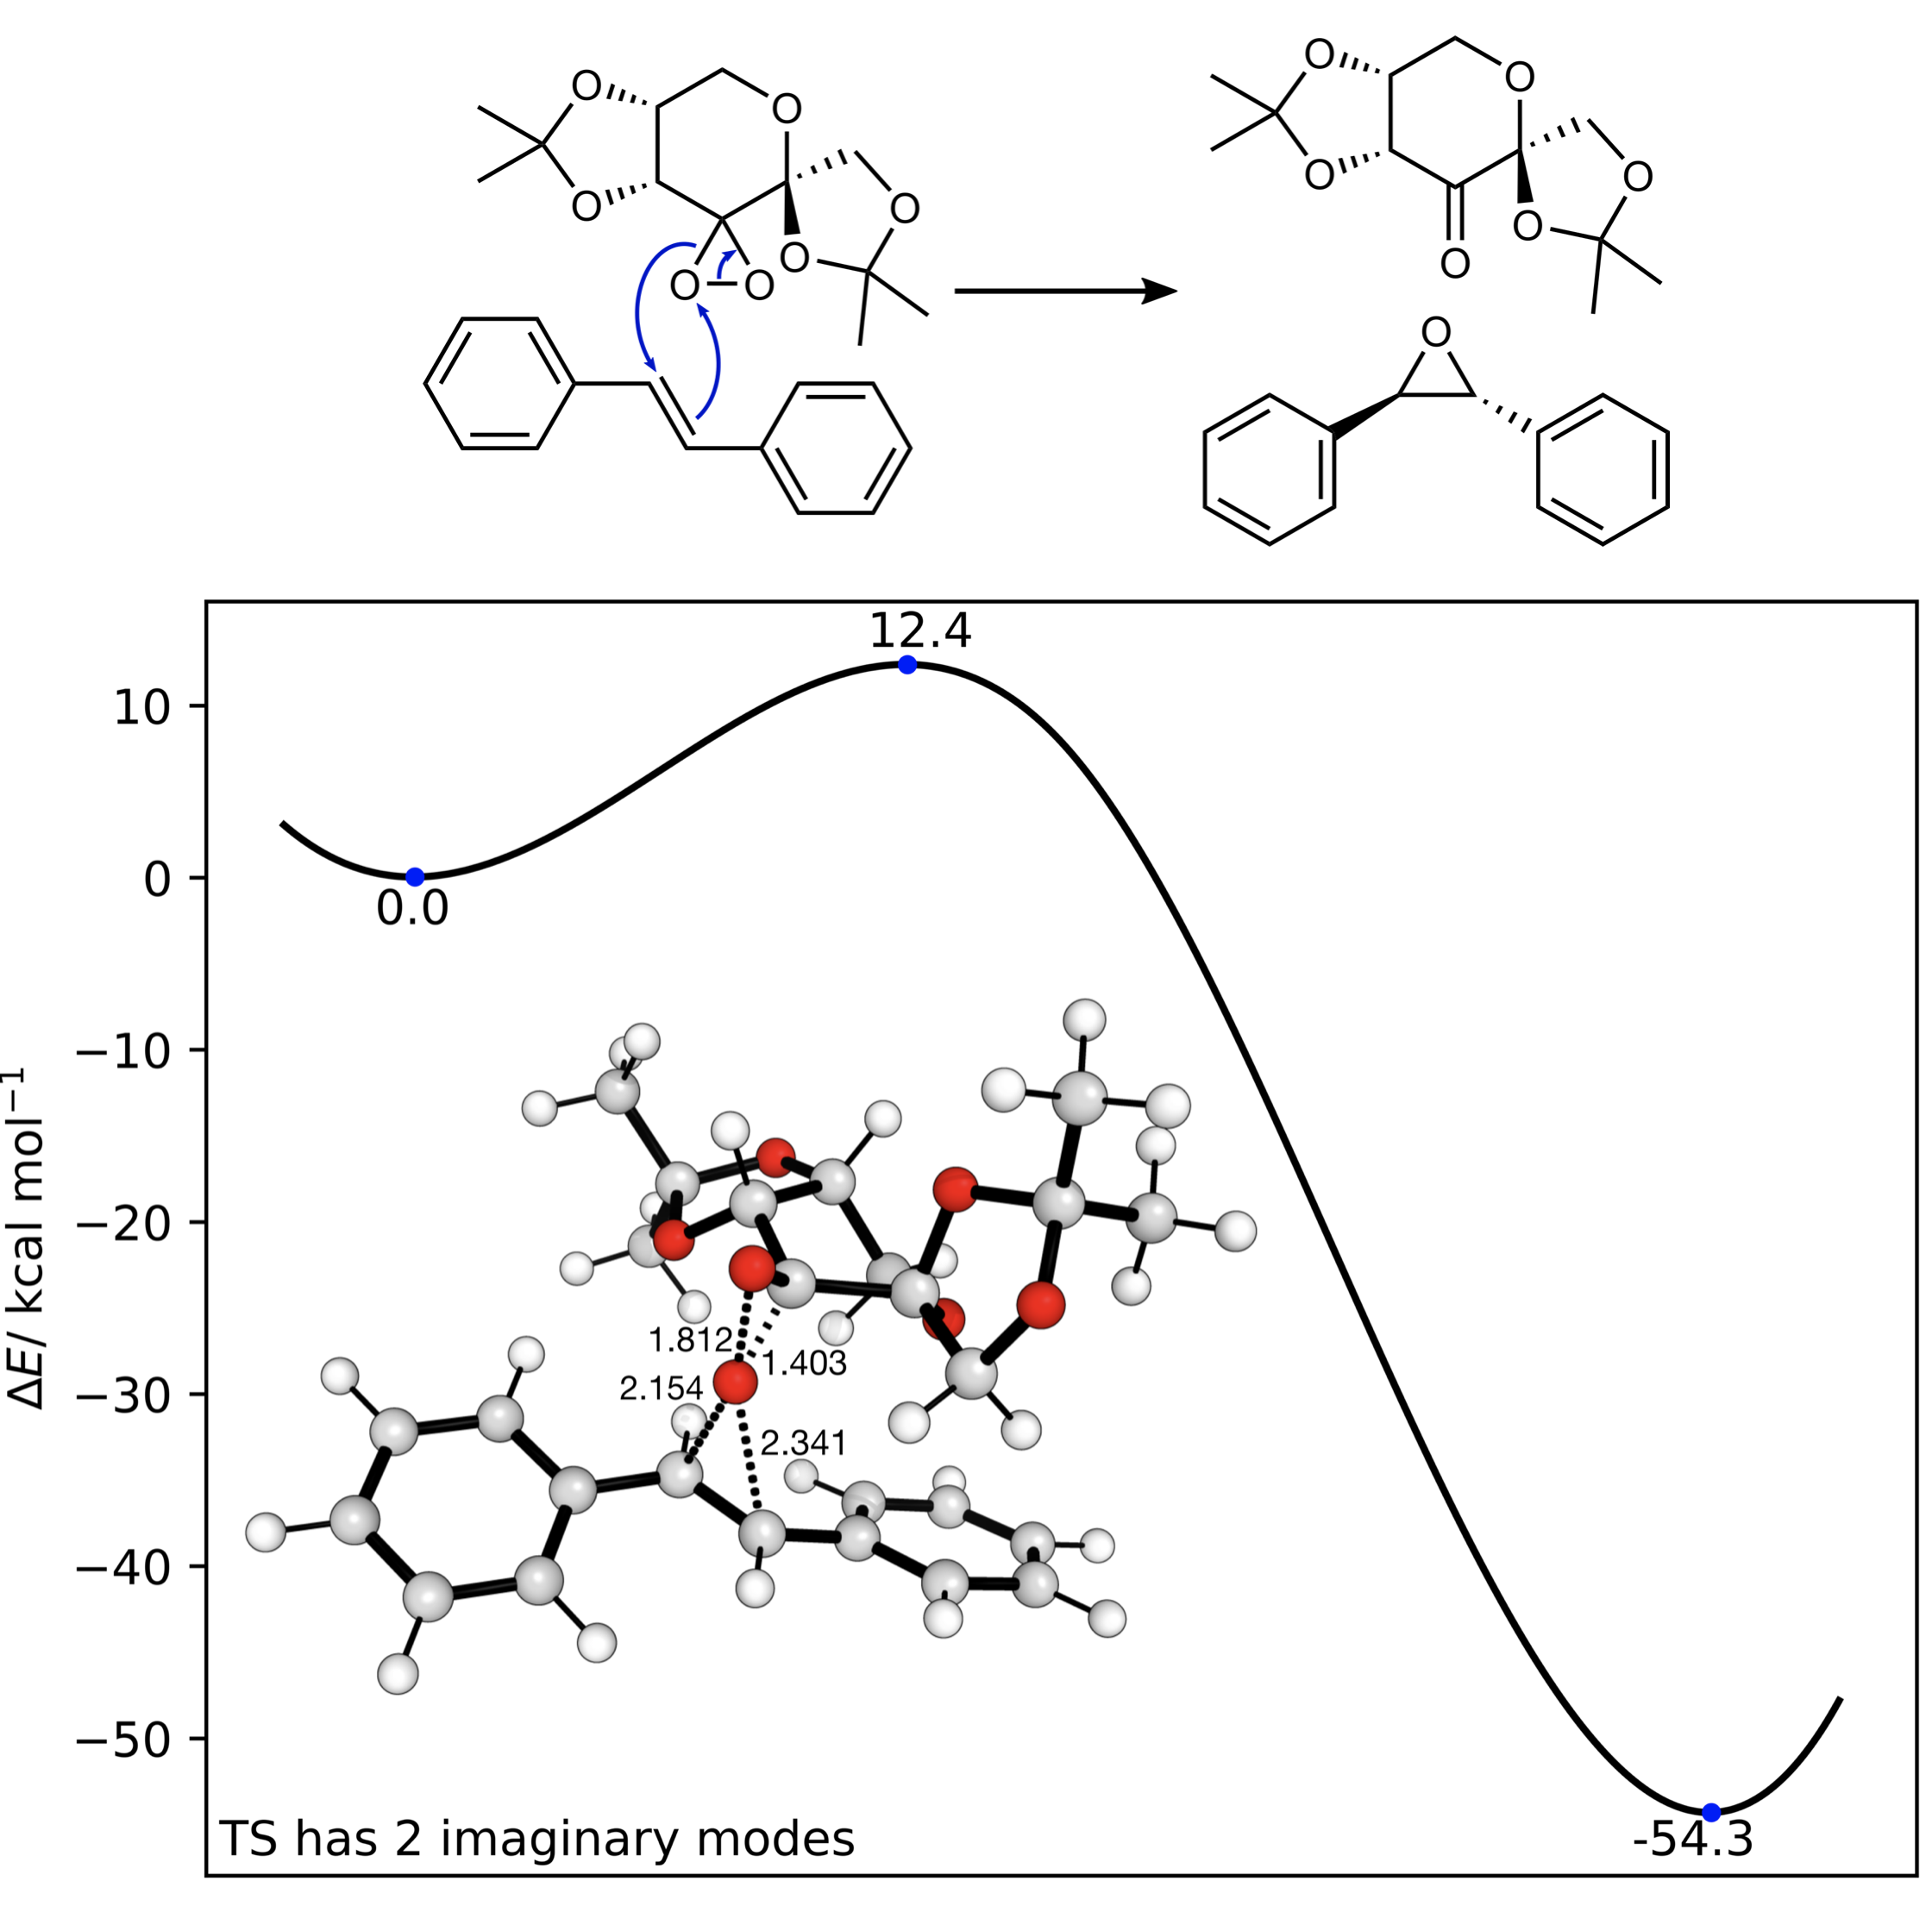
\includegraphics[width=11cm]{5/autode/figs/figS26}
	\vspace{0.2cm}
	\hrule
	\caption{Diastereoselective epoxidation from ref. \cite{Schneebeli2009} generated in \ade (ORCA/XTB, PBE0-D3BJ/def2-TZVP//PBE0-D3BJ/def2-SVP). Second spurious imaginary frequency 7.35$i \text{ cm}^{-1}$.}
	\label{fig::ade_si_26}
\end{figure}

\fi
% --------------------------------------------------------------------------------------------


\clearpage
\end{document}
